\documentclass{ctuthesis}
\usepackage{graphicx}
\usepackage{url}
\usepackage{wrapfig}
\usepackage{lipsum}    
\usepackage{floatrow}
\usepackage{xargs}
\usepackage{setspace}                  
\usepackage[pdftex,dvipsnames,usenames,nonamebreak,table]{xcolor}
\usepackage{booktabs}
\usepackage[colorinlistoftodos,prependcaption,textsize=tiny]{todonotes}
\newcommandx{\unsure}[2][1=]{\todo[linecolor=red,backgroundcolor=red!25,bordercolor=red,#1]{#2}}
\newcommandx{\change}[2][1=]{\todo[linecolor=blue,backgroundcolor=blue!25,bordercolor=blue,#1]{#2}}
\newcommandx{\info}[2][1=]{\todo[linecolor=OliveGreen,backgroundcolor=OliveGreen!25,bordercolor=OliveGreen,#1]{#2}}	
\newcommandx{\improvement}[2][1=]{\todo[linecolor=Plum,backgroundcolor=Plum!25,bordercolor=Plum,#1]{#2}}
\newcommandx{\thiswillnotshow}[2][1=]{\todo[disable,#1]{#2}}

\definecolor{maroon}{cmyk}{0,0.87,0.68,0.32}
\def\justifying{%
	\rightskip=0pt
	\spaceskip=0pt
	\xspaceskip=0pt
	\relax
}

\usepackage{subfig}
\usepackage{multicol}
\usepackage{tcolorbox}
\usepackage[export]{adjustbox}		
\usepackage{tabularx}
\usepackage{array}
\usepackage{tikz}
\usepackage{tikzpagenodes}
\usepackage{fontawesome5}
\def\checkmark{\tikz\fill[scale=0.4](0,.35) -- (.25,0) -- (1,.7) -- (.25,.15) -- cycle;}
\usepackage{colortbl}
\tcbuselibrary{skins}
%\newcolumntype{Y}{>{\raggedleft\arraybackslash}X}
\tcbset{tab2/.style={enhanced,fonttitle=\bfseries,fontupper=\normalsize\sffamily,
		colback=yellow!10!white,colframe=red!50!black,colbacktitle=Salmon!40!white,
		coltitle=black,center title}}
	



%\usepackage{csquotes}
%\renewcommand*{\labelalphaothers}{}

\newtcolorbox{warningbox}[1][]{%
  enhanced jigsaw, % better frame drawing
  borderline west={2pt}{0pt}{red}, % straight vertical line at the left edge
  sharp corners, % No rounded corners
  boxrule=0pt, % no real frame,
  fonttitle={\large\bfseries},
  colframe = {red!25},  
  colback  = {red!10},
  coltitle={red!20!black},  % Black colour for title
  attach title to upper, % Move the title into the box
  #1
}


\ctusetup{
	xdoctype = B,
	xfaculty = FCEyN,
	mainlanguage = czech,
	titlelanguage = czech,
	title-english = {},
	title-czech = {Construcción e implementación de un sistema integral de 
		caracterización de filtros ópticos utilizados en 
		cámaras 
		multiespectrales.},
	department-czech = {Departamento de Física},
	author = {Juan Reto Reynal},
	supervisor = {Prof. Dr. Hernán Grecco},
	supervisor-address = {Laboratorio de Electrónica Cuántica, DF, FCEyN, UBA.},
	month = 5,
	year = 2020,
}


\ctuprocess





\def\ctucaptionsenglish{
	\def\appendicesname{Appendices}
	\def\thanksname{Carátula}
	\def\abstractname{Abstract}
	\def\declarationname{}
	\def\listfigurename{Figures}
	\def\listtablename{Tables}
	\def\supervisorname{Supervisor}
	\def\supervisorspecialistname{Supervisor--specialist}
	\def\fieldofstudyname{Field\ of\ study}
	\def\subfieldofstudyname{Subfield}
	\def\specificationname{Project\ Specification}
	\def\keywordsname{Keywords}
	\def\titletranslationname{Title\ translation}
}

\def\ctucaptionsczech{
	\def\appendicesname{Apéndice}
	\def\thanksname{}
	\def\contentsname{Índice}
	\def\abstractname{Resumen}
	\def\declarationname{}
	\def\listfigurename{Índice de Figuras}
	\def\listtablename{Índice de Tablas}
	\def\supervisorname{Director}
	\def\supervisorspecialistname{\v Skolitel--specialista}
	\def\fieldofstudyname{Obor}
	\def\subfieldofstudyname{Zam\v e\v ren\'i}
	\def\specificationname{Zad\'an\'i\ pr\'ace}
	\def\keywordsname{Palabras clave}
	\def\titletranslationname{P\v reklad\ n\'azvu}
}

\newcommand\Chapter[2]{\chapter[#1]{#1\\[1ex]\large#2}}

\begin{thanks}
	
	\raggedright
	\textsc{TEMA:} Construcción e implementación de un sistema integral de caracterización de filtros
	
	 \hspace{1.6cm}ópticos utilizados en cámaras multiespectrales.
	
	\bigskip
	
	\textsc{ALUMNO:} Juan Reto Reynal
	
	\bigskip
	
	\textsc{L.U. N$^{\circ}$:} 777/12
	
	\bigskip
	
	\textsc{LUGAR DE TRABAJO:} LEC, Departamento de Física, FCEyN, UBA.
	
	
	\bigskip
	
	\textsc{DIRECTOR DEL TRABAJO:} Dr. Hernán E. Grecco
	
	\bigskip
	
	\textsc{FECHA DE INICIACIÓN:} 6 de Mayo de 2019
	
	\bigskip
	
	\textsc{FECHA DE FINALIZACIÓN:} Mayo de 2020
	
	\bigskip
	
	{\large FECHA DE EXAMEN: }
	
	\bigskip
	
	\textsc{INFORME FINAL APROBADO POR:}
	\vspace{2cm}
	
	\begin{center}
		\begin{tabular}{lll}
			\cline{1-1}\cline{1-1}\cline{3-3}\cline{3-3}%
			Autor:  & \hspace{2cm} & Jurada\ \ \ \ \ \ \ \ \ \ \ \ \ \ \
			\ \ \ \ \ \ \ \ \ \ \ \ \ \ \ \  \\
			&& \\
			&& \\
			&& \\
			\cline{1-1}\cline{1-1}\cline{3-3}\cline{3-3}%
			Director: \ \ \ \ \ \ \ \ \ \ \ \ \  & \hspace{2cm} & Jurado\\
			&& \\	
			&& \\
			&& \\
			\cline{1-1}\cline{1-1}\cline{3-3}\cline{3-3}%
			Profesora: Silvina Ponce Dawson  & \hspace{2cm} & Jurado\\
			&& \\
			&& \\
			&& \\
		\end{tabular}	
	\end{center}
\justifying
\end{thanks}

\singlespacing
\begin{declaration}
\spacing{1.5}

\hspace{0.5cm}En la tesis de licenciatura de Agustina Pose \cite{Pose2017}, dirigida 
por Hernán Grecco quien también dirigió esta tesis, ambos evaluaron un prototipo 
de cámaras multi e hiperespectrales para uso satelital junto a la empresa Satellogic. Tras 
la realización de pruebas y mediciones en tierra, se aprobó la 
prueba de concepto del prototipo y se lo adaptó a un diseño robusto. La 
cámara hiperespectral diseñada es hoy una de las cargas útiles (ó 
\textit{payloads}) a bordo de los satélites argentinos NewSat 1 y NewSat 2 
(alias Fresco y Batata), puestos en órbita el 30 de Mayo de 2016, construidos 
por la empresa Satellogic.

\hspace{0.5cm}En la presente tesis se propuso una continuación de dicho trabajo, en colaboración con la empresa Satellogic, a partir del desarrollo de un 
sistema integral de caracterización de los filtros de interferencia de banda 
que son utilizados en las cámaras multiespectrales. Estos filtros permiten el 
paso de las longitudes de onda que se desean capturar con el sensor 
de detección principal de la cámara que sólo detecta intensidad lumínica. En consecuencia, la caracterización de los 
filtros resulta fundamental para garantizar la calidad de las imágenes 
capturadas. 

\end{declaration}


\newcommand{\mychapter}[2]{
    \setcounter{chapter}{#1}
    \setcounter{section}{0}
    \chapter*{#2}	
}


\begin{document}	

\maketitle

\renewcommand{\chaptername}{Capítulo}
\renewcommand{\tablename}{Tabla}
\renewcommand{\figurename}{Figura}
\interfootnotelinepenalty=10000



\setlength{\parindent}{0.5cm}
\setlength{\parskip}{1em}

\chapter{Introducción}
QUÉ ES UN DEFECTO Y QUÉ LE ESTÁ HACIENDO A LAS IMÁGENES, MOSTRAR IMAGEN QUE TIENE PUNTOS CON DIFRACCIÓN, LOS TIFFS..

\vspace{1cm}
\todo[inline]{explicar microscopio, conceptos como apertura numérica.. espectroscopía un poco etc}
\vspace{1cm}

\textsc{Título:} Construcción e implementación de un sistema integral de 
caracterización de filtros ópticos utilizados en cámaras hiperespectrales.


\hspace{-0.4cm}\textsc{Alumno:} Juan Reto Reynal L.U. 777/12.

\hspace{-0.4cm}\textsc{Director:} Dr. Hernán E. Grecco, 
Prof. Adj. UBA, Inv. Indep. CONICET.

\hspace{-0.4cm}\textsc{Lugar de trabajo:} LEC, Departamento de Física, FCEyN, UBA.


\section*{Objetivo general}
\hspace{0.5cm}La espectroscopía de imágenes hiperespectrales, en inglés 
\textit{Hyperspectral 
Spectroscopy Imaging} (HSI), combina la espectroscopía y la adquisición de 
imágenes 
en dos dimensiones. Este método brinda datos espectrales para cada 
pixel en el campo de 
visión\footnote{El campo de visión, en inglés \textit{field of view} (FOV), es 
el ángulo sólido a través del cual un sensor puede detectar la radiación 
electromagnética que se desee capturar.}. A partir de dichos 
datos se puede extraer información sobre la emisión, reflexión ó absorción de 
una muestra, que puede ser utilizada para determinar su 
composición físico-química con una resolución espacial. De esta forma se pueden 
identificar tumores de un cáncer, realizar un control de calidad de la comida 
identificando bacterias en tiempo real, localizar las células de una muestra 
biológica u optimizar la siembra y la cosecha de ciertos cultivos, entre otras 
aplicaciones.




En la tesis de licenciatura de Agustina Pose \cite{Pose2017}, dirigida 
por 
Hernán Grecco quien también dirige esta tesis, ambos desarrollaron un prototipo 
de cámara hiperespectral para uso satelital junto a la empresa Satellogic. Tras 
la realización de pruebas y mediciones en tierra, se aprobó la 
prueba de concepto de este prototipo y se lo adaptó a un diseño robusto. La 
cámara hiperespectral diseñada es hoy una de las cargas útiles (o 
\textit{payloads}) a bordo de los satélites argentinos NewSat 1 y NewSat 2 
(alias Fresco y Batata), puestos en órbita el 30 de Mayo de 2016, construidos 
por la empresa Satellogic.

En el presente proyecto se propone continuar con dicho trabajo y desarrollar un 
sistema integral de caracterización de los filtros de interferencia de banda 
que son utilizados en las cámaras hiperespectrales. Estos filtros permiten el 
paso de las longitudes de onda (colores) que se desean capturar con el sensor 
de detección principal de la cámara que sólo detecta intensidad lumínica, como 
se explica en la Introducción. En consecuencia, la caracterización de los 
filtros resulta fundamental para garantizar la calidad de las imágenes 
capturadas. El primer prototipo de este sistema integral permitirá 
principalmente caracterizar el espectro de transmisión del filtro en 
cada punto del mismo, es decir en cada posición $(x,y)$ de su superficie, y 
encontrar defectos que pudieran modificar su capacidad de bloqueo de ciertas 
longitudes de onda no deseadas.

\subsection*{Objetivos específicos del proyecto}
\label{sec:introdhiper}
\begin{itemize}
	
	\item \texttt{Objetivo 1:} Caracterización de los espectros de transmisión 
	de los filtros.
	\item \texttt{Objetivo 2:} Detección de los defectos de los filtros 
	(\textit{scratch and dig}).
	\item \texttt{Objetivo 3:} Caracterización de los filtros en su posición 
	final en las cámaras de vuelo 
	del satélite. \end{itemize}
\section*{Introducción}

\hspace{0.5cm}Una imagen a color RGB convencional está compuesta por tres 
canales de 
imágenes (bandas): rojo 
($\sim$ 665nm), verde ($\sim$ 550nm) y azul ($\sim$ 470nm). Este tipo de 
imágenes permiten emular la percepción que el ojo humano tiene del color, pero 
en general no permiten la detección e identificación de distintos objetos 
sólidos y 
líquidos, menos 
aún determinar sus propiedades. Para ello 
es necesario obtener el espectro completo del objeto de estudio que es posible 
a partir de la captura de imágenes multiespectrales e hiperespectrales.

Las imágenes multiespectrales contienen un número acotado de bandas espectrales 
de hasta un par de decenas, con un gran ancho de banda (varias decenas de nm); 
mientras que las hiperespectrales están formadas por un gran número de bandas 
espectrales (de cientos a miles), con una resolución espectral muy estrecha, de 
unos pocos nm (Ver Figura \ref{fig:spectrus}).


\begin{figure}[H]
	\centering
	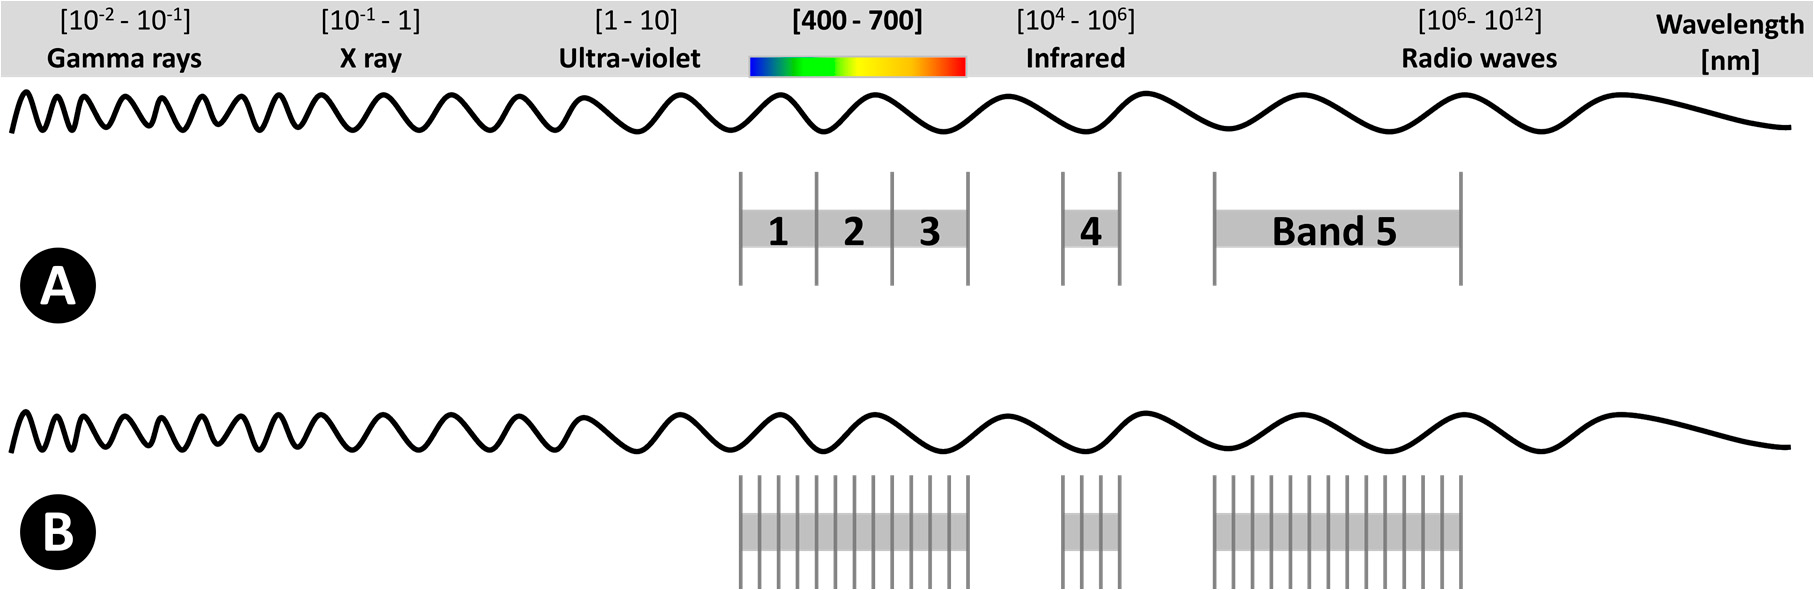
\includegraphics[scale=0.2]{Figs/plan_de_tesis/multivshyper.png}
	\caption{ Representación de los espectros: (A) Multiespectral: 5 
		bandas anchas; y, (B) Hiperespectral: muchas bandas muy estrechas, 
		generalmente entre cientos y miles de ellas. Los dibujos no se 
		encuentran 
		realizados a escala. Imagen tomada de \cite{Adao2017}.}
	\label{fig:spectrus}
\end{figure}


Las cámaras de adquisición de imágenes hiperespectrales estándard utilizan 
redes de difracción o prismas como elementos dispersivos de la luz. La 
distancia requerida entre el sensor de detección y  el componente de difracción 
de la luz, hace que este tipo de cámaras sean muy grandes y muy pesadas, dos 
condiciones que por ejemplo en la industria satelital se quieren optimizar 
fuertemente ya que el costo de la puesta en órbita de los satélites es 
proporcional a su peso y a su tamaño. Estas cámaras suelen ser muy caras y muy 
sensibles a desalinearse debido a las condiciones mecánicas de su construcción. 
Esta última condición se agrava en sistemas de difícil manipulación como lo son 
los satélites, que una vez que se encuentra en órbita, sus componentes ópticos 
ya no puede ser modificados como para corregir una desalineación que empeore la 
calidad de las imágenes capturadas. Además, requieren de una rendija 
para poder obtener una alta resolución espectral, lo que restringe 
significativamente la intensidad de la luz a detectar.

En respuesta a las desventajas de las cámaras estándard de imágenes 
hiperespectrales, aparecieron otro tipo de cámaras que utilizan filtros de 
interferencia de banda y que resultaron en un producto final robusto, compacto, 
de bajo costo y de muy buen rendimiento. Una cámara de vuelo 
de este tipo fue desarrollada en la tesis de licenciatura de Agustina Pose bajo 
la dirección de Hernán Grecco \cite{Pose2017} como se mencionó anteriormente. 
La cámara desarrollada tiene la gran ventaja de no presentar partes móviles, 
evitando posibles desalineaciones de los componentes ópticos. Las partes 
móviles de la cámara que serían útiles para realizar un barrido espectral de 
una cierta escena a capturar, no son necesarias pues el barrido es realiizado 
por el movimiento propio del satélite respecto de la Tierra. El esquema básico 
de este tipo de 
cámaras hiperespectales se muestra 
en la Figura \ref{fig:camsens}. Los filtros de interferencia de banda 
utilizados en este tipo de cámaras deben cumplir ciertos requisitos de calidad 
(no presentar rayones, ni marcas, etc) 
y ciertas características espectrales y de transmisión antes de ser 
incorporados a la carga útil de, por ejemplo, un satélite que va a ser puesto 
en 
órbita. En consecuencia, resulta fundamental caracterizar completamente dichos 
filtros antes de construir las cámaras de la aplicación de interés.

\begin{figure}[H]
	\centering
	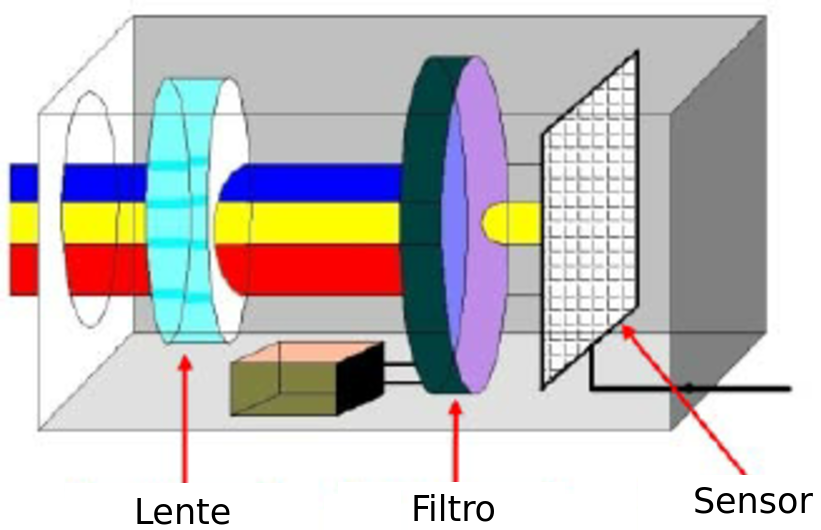
\includegraphics[scale=0.535]{Figs/plan_de_tesis/cam_sens.png}
	\caption{ Esquema de una cámara hiperespectral. El filtro absorbe el 
	espectro completo de la luz incidente salvo la banda espectral que el 
	usuario determina, por lo que sólo las longitudes de onda elegidas 
	atraviesan el filtro y son detectadas por el sensor. \cite{Martinez2008}}
	\label{fig:camsens}
\end{figure}



Debido a las limitaciones de las técnicas de 
medición estándard 
de los espectros de transmisión de los filtros ópticos donde se utilizan 
espectrómetros comerciales, existen tres discrepancias fundamentales 
entre el espectro ''real''\footnote{El espectro ''real'' es 
	el espectro de diseño del filtro para el que fue especialmente construido.} 
	de 
un 
filtro y sus mediciones experimentales realizadas con 
espectrómetros comerciales (Ver Figura \ref{fig:obj1a})\cite{Semrock}. La 
primera discrepancia es el "redondeo" de características espectrales nítidas de 
los filtros. 
Esto se debe al ancho de banda no nulo del haz de la sonda del 
espectrómetro. 


La segunda discrepancia se debe al rango limitado de 
medición de la OD\footnote{La densidad óptica, OD (Optical Density), es un 
	parámetro útil para describir la transmisión de la luz a través de un 
	filtro 
	óptico con una transmisión extremedamente baja. Si T es la transmisión del 
	filtro, que varía entre 0 y 1, se define la densidad óptica como $OD = 
	-$log$_{10} (T)$.} del filtro, que es 
producto de la sensibilidad limitada del espectrómetro. Cuando un filtro 
tiene un valor de OD muy alto, OD $>$ 6, el detector debería medir una 
intensidad de la luz prácticamente nula pero el ruido óptico y electrónico 
propio del detector limita el nivel más bajo de intensidad que puede medir 
con precisión. De esta forma, se puede ver un ruido de piso debido al 
sensor indicando un cierto valor de OD que no coincide con el valor real 
del filtro.

\begin{figure}[H]
	\centering
	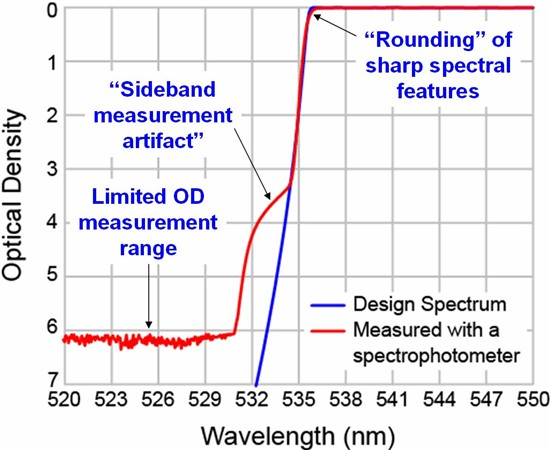
\includegraphics[scale=0.8]{Figs/plan_de_tesis/measurement_of_optical_filter.jpg}
	\caption{Discrepancias entre las mediciones experimentales con 
		espectrómetros 
		comerciales y el espectro ''real'' de un filtro óptico. Adaptado de 
		\cite{Semrock}.}
	\label{fig:obj1a}
\end{figure}

La tercera 
discrepancia es propia de las mediciones de transiciones muy 
pronunciadas. Esto surge 
por el hecho de que el 
haz de la sonda no es monocromático, sino que también tiene bandas 
laterales débiles de longitudes de onda fuera de su ancho de banda 
principal.

Las discrepancias de medición en espectrómetros convencionales 
causan 
importantes problemas al intentar evaluar el rendimiento del filtro para la 
aplicación prevista. 

La elección del instrumento de medición y la técnica 
empleada determinan la precisión de la medición del espectro de transmisión del 
filtro. Al mismo tiempo, determinan la duración y por ende también el costo de 
dichas mediciones, que deben ser compatibles con los tiempos que la industria 
requiere. Esto se puede ver con un ejemplo tomado de \cite{Semrock}. En la 
Figura \ref{fig:may_dists} se muestran cinco mediciones distintas de 
la densidad óptica de un filtro diseñado para bloquear longitudes de onda de 
532 nm con OD $>$ 6 y tener una transición a un estado de alta transmisión 
dentro del $0.5\%$ de la longitud de onda del láser utilizado para excitar la 
muestra, que es de 534.7nm.


\begin{figure}[H]
	\centering
	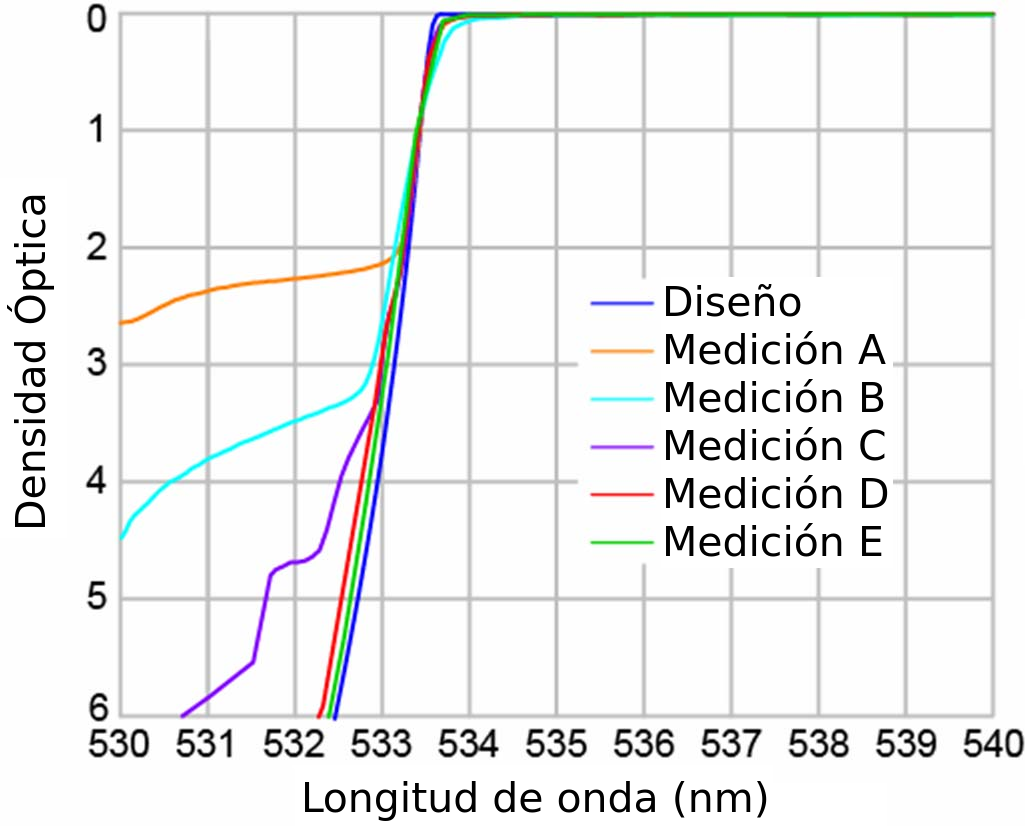
\includegraphics[scale=0.8]{Figs/plan_de_tesis/dists_meds.png}
	\caption{Distintas mediciones de la OD de un filtro LP03-532RE-
		25 RazorEdge de la empresa Semrock. Las mediciones fueron realizadas 
		utilizando tanto espectrómetros comerciales como \textit{custom-made} 
		de la emppresa con una variedad de arreglos experimentales que se 
		explican en el texto. Adaptado de 
		\cite{Semrock}.}
	\label{fig:may_dists}
\end{figure}

Las mediciones del método A fueron realizadas por un espectrómetro de diseño 
propio (\textit{custom-built}) de la empresa,  que tiene un tiempo de 
integración muy corto y una baja resolución, lo que resulta en una 
configuración 
experimental óptima para obtener mediciones de una gran cantidad de filtros de 
prueba. Este método es utilizado para determinar con precisión la longitud de 
onda a partir de la cual el filtro pasa a tener una alta transmisión, es decir, 
localiza la longitud de onda de la transición entre el estado de bloqueo y de 
transmisión del filtro, la longitud de onda de corte. De esta forma, se 
garantiza una cierta uniformidad en un lote de filtros a ser utilizado de una 
forma rápida y eficiente. Ahora bien, como se observa en el gráfico de la 
Figura \ref{fig:may_dists}, el método A posee una sensibilidad muy mala y una 
resolución muy baja, obteniéndose un piso de ruido mayor a OD 2.

El método B utiliza un espectrómetro comercial (Perkin Elmer
Lambda 900) cuyos inconvenientes fueron explicados a partir de las tres 
discrepancias en la Figura \ref{fig:obj1a}. Con este método no se puede 
asegurar que el filtro tenga un 0D $>$ 6 en los 532nm.


Los métodos C y D utilizan el mismo espectrómetro \textit{custom-built}	del 
método A, cuyo principio de funcionamiento básico se muestra en la Figura 
\ref{fig:med_prev}. La diferencia fundamental con el método B que utiliza un 
espectrómetro comercial es que las mediciones con el espectrómetro 
\textit{custom-built} realizan la detección con una cámara CMOS de bajo ruido, 
que consiste en un arreglo de detectores, por lo que puede medir en un rango 
muy grande de longitudes de onda simultáneamente. Este método permite en 
consecuencia obtener mediciones en un rango espectral muy grande, con una 
cierta resolución en un cierto tiempo de integración, de forma muy rápida.
El inconveniente fundamental de este método es que al utilizar una fuente de 
iluminación de banda ancha, si el filtro de prueba tuviera, por ejemplo, una 
autofluorescencia apreciable \cite{Shah2017}, podría interferir con una 
medición precisa de la transmisión de la muestra.


\begin{figure}[H]
	\centering
	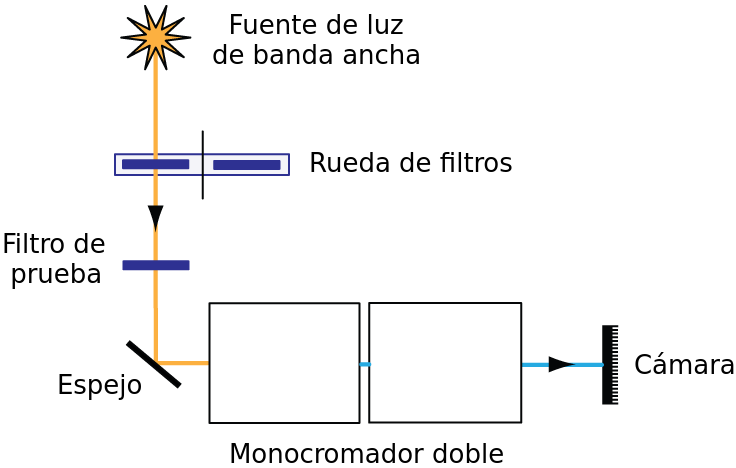
\includegraphics[scale=0.8]{Figs/plan_de_tesis/med_mets_prevs.png}
	\caption{Diseño básico de un espectrómetro \textit{custom-built} que 
	utiliza una fuente de iluminación de banda ancha y permite la recolección 
	de una 		amplia gama de
		longitudes de onda simultáneamente con un conjunto de detectores 
		situados en la cámara. Este 
		arreglo experimental permite una medición más rápida con un piso de 
		ruido y una resolución fijas. Adaptado de 
		\cite{Semrock}.}
	\label{fig:med_prev}
\end{figure}




Ahora bien, dependiendo de la aplicación, las limitaciones en las mediciones 
del espectro de transmisión de los filtros pueden ser determinantes o no. En el 
presente proyecto se quiere determinar el arreglo experimental óptimo pero que 
sea compatible con los tiempos y costos de producción de la industria satelital.

En ciertos filtros y aplicaciones, resulta de vital importancia 
el 
nivel de bloqueo de ciertos rangos de longitudes de onda pero no así la 
suavidad de la transición entre el bloqueo y la transmisión. Por ejemplo, en 
sistemas de 
imágenes de fluorescencia los espectros de absorción y emisión del fluróforo 
podrían estar lo suficientemente alejados como para que resulte fundamental que 
los filtros de banda de la señal de respuesta (de emisión) de la muestra tengan 
un bloqueo muy alto en la banda de la señal de excitación y así lograr una 
relación entre la señal y el ruido de adecuada proporción \cite{Grecco2016}. 

Los filtros 
diseñados para estas aplicaciones podrían tener decenas de OD de bloqueo pero 
en 
la práctica incluso el más pequeño de los defectos físicos en los 
recubrimientos ópticos (\textit{coatings}) o en el montaje, así como el bajo 
nivel de control de luz parásita a nivel del sistema, puede limitar el 
bloqueo alcanzable a valores mucho menores que los del diseño original, en el 
rango de aproximadamente OD 6 a quizás 10.%(forma indirecta de medir los scrath 
%and dig!!**))) 

Dado que los espectrómetros 
comerciales estándard tienen una medición de OD de rango limitado debido al 
ruido de fondo del instrumento, se propone un arreglo experimental inicial para 
poder medir los niveles de bloqueo más altos con precisión como se muestra en 
la Figura \ref{fig:su} y que resulta compatible con la producción industrial 
deseada por su simplicidad.


\begin{figure}[h!]
	\centering
	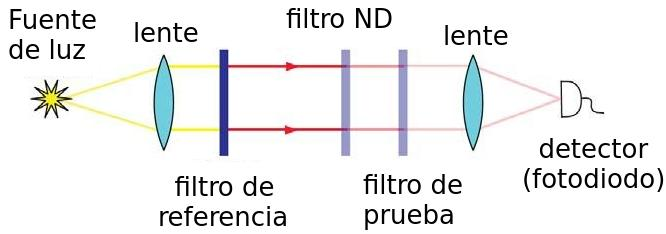
\includegraphics[scale=1.0]{Figs/plan_de_tesis/setup_u.jpeg}
	\caption{Arreglo experimental compatible con la producción industrial para 
	medir valores de 
	OD altos.}
	\label{fig:su}
\end{figure}

El método experimental de la Figura \ref{fig:su} se denomina 
\textit{complementary filter method}. Un haz de 
luz de banda ancha, de una lámpara QTH 
(\textit{Quartz-Tungsten Halogen}) ó de arco, aproximadamente colimado por una 
lente  es filtrado utilizando un filtro 
de referencia ampliamente bloqueador, que es esencialmente un filtro de banda 
con su banda de paso superpuesta a la región del espectro del filtro de prueba 
que se quiere analizar donde la medición de valores de OD altos son necesarios. 
La luz transmitida es enfocada con una lente convergente en un detector de bajo 
ruido capaz de medir niveles de intensidad de luz muy pequeños, como un 
fotodiodo de gran área con un circuito amplificador de bajo ruido ó un tubo 
fotomultiplicador (PMT).


Las mediciones se realizan de la siguiente manera. En primer lugar, se mide la 
intensidad de la señal en el detector con solo el filtro de referencia y un 
filtro calibrado de densidad neutra (ND) en la trayectoria de la luz. El filtro 
ND sirve para reducir el nivel de la intensidad de la luz en el detector en 
una cantidad calibrada de forma tal que el bias \footnote{El bias del 
detector es el valor medido por el instrumento cuando no hay ninguna fuente 
de luz incidiendo sobre él, es el valor de \textit{offset} que se le suma a 
cualquier 
medición.} del rango 
dinámico limitado alcanzable por el detector sea reducido para alcanzar los 
niveles de la señal que el detector va a ver cuando se coloquen los filtros de 
prueba. En particular, con un filtro ND 3, el rango dinámico del detector tiene 
que ser de $10^{6}$ para medir hasta un valor de OD 9 de bloqueo. En segundo 
lugar, se retira el filtro ND y se lo reemplaza por el filtro de prueba para 
realizar una nueva medición de la intensidad con el detector. El cociente entre 
las dos mediciones de intensidad de la luz es igual al valor de OD del filtro 
de prueba, en el rango espectral del filtro de referencia.


\section*{Actividades y Metodología}

\hspace{0.5cm}En el presente trabajo de tesis se desarrollarán múltiples 
arreglos 
experimentales para caracterizar el espectro de transmisión de distintos 
filtros de prueba que dispone el LEC, utilizando técnicas de medición en línea 
con los papers y patentes de la actualidad. Se automatizará la adquisición de 
las mediciones y se incorporará al arreglo experimental inicial un sistema de 
detección de defectos de los filtros, utilizando una cámara de bajo costo del 
laboratorio para realizar las primeras pruebas. 

Una vez caracterizado tanto el espectro como los defectos de los filtros, se 
diseñará y construirá un primer prototipo de un sistema integral de 
caracterización para ser aplicado con los filtros que utiliza la empresa 
Satellogic en sus cámaras hiperespectrales. Se estudiará la aplicabilidad de 
este prototipo en distintos casos.

Utilizando el prototipo del sistema integral de caracterización de los filtros 
se desarrollará un método y criterios para decidir si un filtro puede ser 
incorporado a la cámara utilizada en los satélites.

Como aplicación de este proyecto de tesis se utilizarán las cámaras 
hiperespectrales de la empresa Satellogic, cuyos filtros van a ser 
caracterizados con el sistema integral que se va a desarrollar, y se tomarán 
imágenes en tierra utilizando algoritmos de HDR y de búsqueda de 
características.  Y, finalmente se realizará una caracterización de los filtros 
en su posición final en las cámaras de vuelo del satélite.



\section*{Factibilidad}

\hspace{0.5cm}El lugar de trabajo donde el tesista va a desarrollar sus 
actividades es el 
Laboratorio de Electrónica Cuántica (LEC) del Departamento de Física de la 
Facultad de Ciencias Exactas y Naturales, UBA. El LEC cuenta con diversos 
equipos de uso general en óptica y electrónica y algunos de uso específico para 
aplicaciones en investigación de física básica. Entre los equipos de uso 
relevante para el presente proyecto se pueden encontrar mesas ópticas de 
suspensión neumática, un microscopio invertido automático Zeiss Observer Z1, 
diversas placas de adquisición y procesamiento (NI y Red Pitaya, Raspberry Pi y 
Arduino), cámaras científicas y de bajo ruido (Apogee U2000, QHY183M), 
elementos de óptica para la construcción de instrumentos (lentes, filtros, 
objetivos de microscopio, optomecánica, láseres y leds). Adicionalmente, el 
laboratorio cuenta con acceso a un microscopio confocal de la firma Olympus, 
modelo FV1000 equipado con una platina motorizada, cámara ambiental y cámara 
CCD.
 
El director de la presente tesis es director del LEC y es experto en temas de 
óptica y fotofísica, áreas principales del proyecto. Además, tiene la 
experiencia de haber dirigido a una estudiante que realizó la tesis en conjunto 
con el LEC y la empresa Satellogic, resultando en una experiencia exitosa.

El tesista se encuentra cursando actualmente sus últimas dos materias de la 
carrera: 
Estructura de la Materia 4 e Instrumentación y Control.

%%%%%%%%%%%%%%%%%%%%%%%%%%%%%%%%%%%%%%%%%%%%%%%%%%%%%%%%%%CAPITULO 3:%%%%%%%%%%%%%%%%%%%%%%%% Cuantificación de los defectos a partir de las imágenes tomadas con el ZEISS con scikit-image y OpenCV %%%%%%%%%%%%%%%%%%%%%%%%%%%%%%%%%%%%%%
%%%%%%%%%%%%%%%%%%%%%%%%%%%%%%%%%%%%%%%%%%%%%%%


\singlespacing
\Chapter{Cuantificación de los defectos}{\textcolor{MidnightBlue}{\faGithub \href{https://github.com/jrr1984/defects_analysis}{\texttt{defects$\_$analysis}}}}
\label{chap:zeiss}
\spacing{1.5}

\hspace{0.5cm}La industria óptica ha desarrollado a lo largo de su historia distintas normativas para especificar la calidad de la superficie óptica de un componente \cite{cosm}. Debido a los requerimientos específicos de la industria de imágenes satelitales, dichas normativas suelen ser insuficientes para anticipar las consecuencias que traen los defectos de un componente óptico en el proceso de formación de imágenes de cámaras hiper y multiespectrales.

En este capítulo se define qué es lo que se considera un defecto de un componente óptico [\ref{sec:defectsurf}], las especificaciones técnicas de las normativas más utilizadas de la industria óptica [\ref{sec:scanddig},\ref{sec:iso10110}]. Se muestran las características del filtro óptico analizado en el presente trabajo [\ref{sec:carfilt}]. Se explica el proceso de adquisición de imágenes de microscopía [\ref{sec:conf},\ref{subs:tilsc}] del filtro completo [\ref{subs:compl}] y de cada banda espectral [\ref{sec:cadab}]. Se muestra el proceso de corrección de la iluminación no uniforme del microscopio [\ref{sec:ilumnou}]  que consistió en la generación de una imagen de fondo [\ref{sec:preproc},\ref{sec:genimf}] que a su vez fue utilizada para la normalización de las imágenes adquiridas [\ref{subs:nm}].

Asimismo, se detalla el algoritmo utilizado para realizar la detección de los defectos en las imágenes normalizadas [\ref{sec:tthresh},\ref{sec:secalg}]. Se explica la aplicación de los criterios de normas de calidad a los resultados del algoritmo [\ref{sec:resgrl},\ref{sec:sctdig},\ref{sec:apiso}] y posteriormente se muestran los resultados de caracterización de los defectos denominados agujeros [\ref{sec:aguj}]. Luego se muestran los resultados de la población de defectos [\ref{sec:defpob}]; lo cual permitió establecer los criterios de diseño del microespectrómetro detallado en el Capítulo \ref{chap:microsp}. Finalmente, se explica la asociación de incertezas a los resultados del algoritmo [\ref{sec:incert}].

%%%%%%%%%%%%%%%%%%%%%%%%%%%%%%%%%%%%%%%%%%%%%%%%%%%%%%%%%%%%%%%%%%%%%%%%%%%%%%%%%%%%%%%%%%%%%%%%%%%%%%%%%%%%%%
\singlespacing
\section{Defectos de superficie de un componente óptico}
\label{sec:defectsurf}
\spacing{1.5}

\hspace{0.5cm}Se define un defecto de superficie de un componente óptico de manera general como una ruptura de la homogeneidad de la superficie óptica \cite{Gomez_1998}. Estas imperfecciones localizadas consisten de rayaduras, huecos, manchas, burbujas entre otras. La terminología varía dependiendo del sector de la industria óptica que se trate. En particular, en el presente trabajo se caracterizaron defectos de superficie denominados en adelante agujeros ó huecos (Ver Figura \ref{fig:huecoazul}) y manchas ó defectos de transmisión (Ver Figura \ref{fig:manchaazul}).  

\begin{figure}[H]
	\begin{floatrow}
		\ffigbox{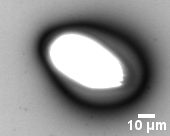
\includegraphics[width=4.0cm,height=4.0cm]{Figs/cuantificaciondefectos/hueco_cel_112.png}}{\caption{Defecto de superficie denominado agujero ó hueco, de (37 $\pm$ 1)$\mu$m de diámetro equivalente. }\label{fig:huecoazul}}
		\ffigbox{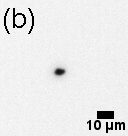
\includegraphics[width=4.0cm,height=4.0cm]{Figs/cuantificaciondefectos/mancha_inicio.png}}{\caption{Defecto de superficie denominado mancha ó defecto de transmisión, de (6 $\pm$ 1)$\mu$m de diámetro equivalente.}\label{fig:manchaazul}}
	\end{floatrow}
\end{figure}

Los defectos de superficie de un componente óptico pueden originarse en el proceso de fabricación mismo, en el tratamiento y manipulación de la óptica (en inglés, \textit{handling}), en distintas etapas de un proceso de montaje ó en el transporte del proveedor al cliente. Estos defectos pueden provocar un cambio de las propiedades ópticas del componente y en consecuencia los usuarios deben verificar la calidad óptica que los proveedores detallan en las especificaciones técnicas. A continuación se describen las especificaciones técnicas más utilizadas en la industria para determinar la calidad óptica de un componente:\textit{U.S. Military Performance Specification} MIL-PRF-13830 \cite{milprf}y ISO 10110 \cite{iso10110}. Ambas especificaciones fueron indicadas en la hoja de datos del filtro analizado en el presente trabajo.
%%%%%%%%%%%%%%%%%%%%%%%%%%%%%%%%%%%%%%%%%%%%%%%%%%%%%%%%%%%%%%%%%%%%%%%%%%%%%%%%%%%%%%%%%%%%%%%%%%%%%%%%%%%%%%%%%%%%%%%%%%%%%%%%%%%%%%%%%%%%%%%%%%%%%%%%%%%%%%%%%%%%%%%%%%%%%%%%%%%%%%%%%%%%%%%%%%%%%%%%%%%%%%%%%%%%%%%%%%%%

\singlespacing
\subsection{MIL-PRF-13830: especificaciones de \textit{scratch \& dig}}
\label{sec:scanddig}
\spacing{1.5}

\hspace{0.5cm}La especificación técnica MIL-PRF-13830 define un \textit{scratch} (en adelante rayadura) como cualquier marca o rayadura de la superficie óptica del componente y un \textit{dig} (en adelante, simplemente defecto) como cualquier otro defecto de superficie presente en la óptica, como por ejemplo el agujero ó hueco de la Figura \ref{fig:huecoazul} ó el defecto de transmisión ó mancha de la Figura \ref{fig:manchaazul}. Esta reglamentación define las rayaduras y defectos permitidos en una superficie óptica utilizando una métrica dada por un par de números denominados \textit{scratch and dig numbers}: S/D. El \textit{scratch number} puede tomar alguno de los siguientes valores arbitrarios: 5,10,20,40,60,80, que representan en orden creciente el nivel de brillo de la rayadura. Este número no proviene de una medición experimental, sino que es el resultado de comparar el brillo de la rayadura del componente a analizar con muestras de rayaduras calibradas, como las que se muestran en la Figura \ref{fig:scratchanddig}, bajo ciertas condiciones de iluminación específicas (Ver \textit{Inspection method's}: 4.2.2.1 y 4.2.2. \cite{milprf}).
\begin{figure}[H]
	\centering
	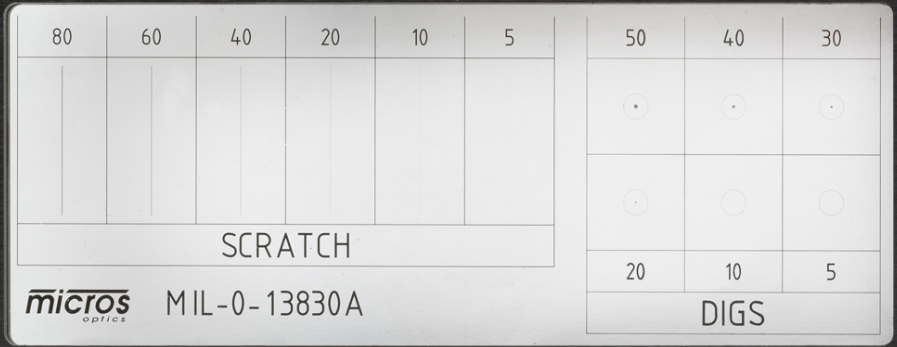
\includegraphics[scale=0.8]{Figs/cuantificaciondefectos/paddlecalibration.png}
	\caption{Muestra calibrada de \textit{scratch \& dig} comercializada por la empresa Thorlabs. Adaptado de \href{https://www.thorlabs.com/newgrouppage9.cfm?objectgroup_id=1427&pn=MOTP-MIL}{\texttt{https://bit.ly/3bPSMYS}}.}
	\label{fig:scratchanddig}
\end{figure}
El \textit{dig number} es el diámetro del defecto más grande permitido en el componente, dado en $1/100$ de milímetros. Por ejemplo, un componente con un \textit{dig number} de 40 implica que los defectos más grandes de la óptica pueden ser de un diámetro de hasta 0.4 mm. Si bien el \textit{dig number} es una cantidad medible experimentalmente, con por ejemplo, un microscopio, también se utilizan muestras calibradas para determinar el tamaño y cantidad de los defectos (Ver Figura \ref{fig:scratchanddig}). Luego de que un inspector entrenado cuantifica todas las rayaduras y defectos de la óptica con las muestras calibradas, se verifica la calidad óptica del componente de acuerdo a los siguientes criterios:
\begin{itemize}
\item La suma de todas las longitudes\footnote{La longitud es medida con una regla metálica (\textit{NIST traceable steel ruler}). En el caso de que la rayadura sea curva, su longitud es estimada por el inspector \cite{Aikens}.} de las rayaduras con el \textit{scratch number} (L$_{S_{\#}}$) asociado (máximo valor de brillo permitido) no podrá superar el valor de un cuarto del diámetro ($\Phi$) de la óptica. Si el componente no tuviera una geometría circular, se considera el diámetro de un círculo con un área igual al de la óptica bajo análisis.
\begin{equation}
\sum L_{S_{\#}} < \frac{\Phi}{4}
\label{eq:snumb}
\end{equation}
\item El número total (N) de defectos con el \textit{dig number} asociado (máximo diámetro de los defectos pemitido) no podrá exceder el diámetro de la óptica dividido por 20 mm. De obtenerse un número no entero, se trunca el resultado.
\begin{equation}
N  <  \frac{\Phi}{20 mm}
\label{eq:nphi20}
\end{equation}
\item La suma de todos los diámetros (d) de los defectos deberá ser menor ó igual al doble del número total de defectos de diámetro máximo permitido (N) multiplicado por el \textit{dig number} (D$_{\#}$), dado en $1/100$ de milímetros.
\begin{equation}
\sum d 	\leq 2 . N . D_{\#}
\label{eq:dmenorig}
\end{equation}
\end{itemize}
\hspace{0.5cm}Así por ejemplo, una óptica de geometría circular con un diámetro de 200 mm y una calidad óptica especificada por el fabricante con \textit{scratch and dig numbers} S/D 30-20, podrá tener rayaduras con un brillo calibrado de 30 y la suma de todas las longitudes de las rayaduras de brillo 30 no podrá ser superior a los 50 mm (de acuerdo a \eqref{eq:snumb}). Al mismo tiempo, la óptica no podrá tener más de 10 defectos de \textit{dig number} igual a 20, es decir de tamaño máximo de 0.2 mm (de acuerdo a  \eqref{eq:nphi20}) y la suma de los diámetros de todos los defectos no podrá ser superior a los 4 mm (de acuerdo a \eqref{eq:dmenorig}).

La Figura \ref{fig:samplescratchs} muestra una comparación de cuatro muestras de calibración de rayaduras, medidas bajo idénticas condiciones de iluminación \cite{Aikens}.
\begin{figure}[H]
	\centering
	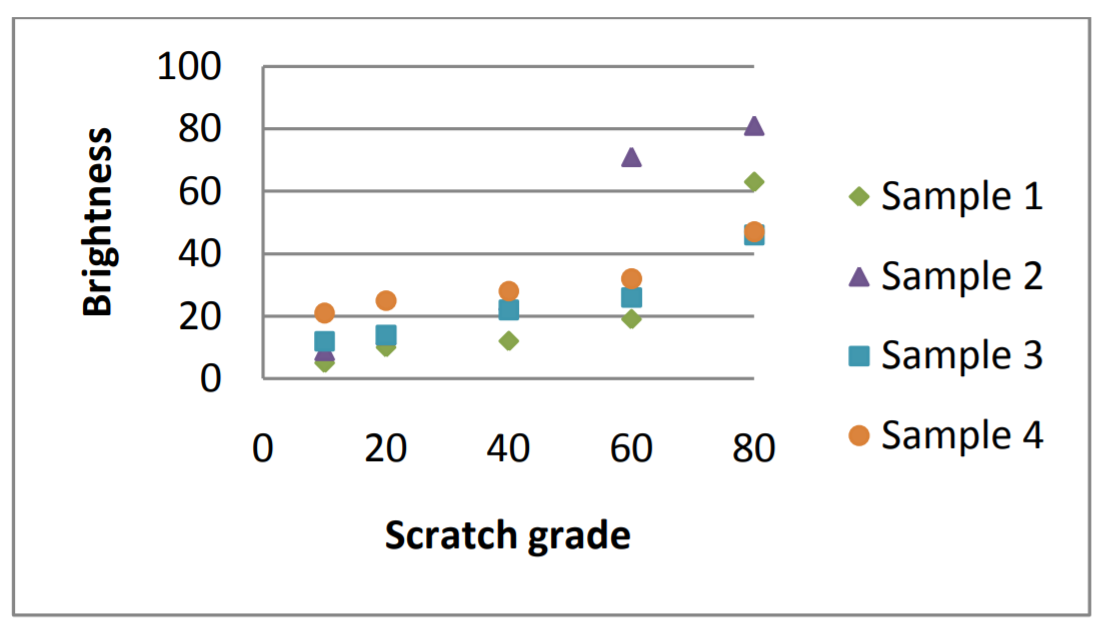
\includegraphics[scale=0.54]{Figs/cuantificaciondefectos/samplesscratch.png}
	\caption{Brillo relativo de cuatro muestras calibradas de \textit{scratch number}. \textit{Sample} en inglés significa muestra. La muestra 1 es de la empresa FLIR/Brysen (S\&D 1109), la muestra 2 es de Davidson Optronics (D-667A S/N 2431), la muestra 3 es de Eastman Kodak (\textit{paddle} EKCO CM2) y la muestra 4 es de Jenoptik (\textit{paddle} EO \#53-157 CM1). Gráfico tomado de \cite{Aikens}.}
	\label{fig:samplescratchs}
\end{figure}
De la Figura \ref{fig:samplescratchs} se desprende que las cuatro muestras son incompatibles entre sí, es decir arrojan resultados de brillo distintos entre sí para un cierto \textit{scratch number}. Se observa que para un \textit{scratch number} igual a 10, el brillo de la muestra 4 es de mayor intensidad que el \textit{scratch number} 60 de la muestra 1.
Así también el brillo del \textit{scratch number} 60 de la muestra 2 es más de dos veces más brillante que cualquiera de las otras muestras para este mismo \textit{scratch number}.

Además, la métrica de \textit{scratch \& dig} tiene la falencia de no poder caracterizar ni rayaduras de brillo menores al \textit{scratch number} igual a 5 ni defectos con un \textit{dig number} menor a 5, es decir que en esta métrica no se consideran defectos de diámetro menores a los 50 $\mu m$ \cite{quentin}. Esto es así pues esos números de \textit{scratch \& dig} son los valores más chicos presentes en las muestras calibradas para la inspección visual de acuerdo a los dibujos técnicos oficiales de la métrica (Ver \cite{dibujito})  .

Si bien la métrica de \textit{scratch and dig} sigue siendo ampliamente utilizada en la industria, el hecho de que el análisis de las rayaduras y defectos sea dependiente del inspector de turno sumado a que las muestras de brillo calibradas varían de acuerdo al fabricante de las mismas y que sólo sean considerados defectos con un diámetro mínimo de 50 $\mu m$, hacen que esta especificación técnica para determinar la calidad de una óptica resulte técnicamente ambigua e imprecisa.  A continuación se detallan las especificaciones técnicas de la norma ISO 10110 que supera estas limitaciones. %Luego se muestran las características del filtro analizado en esta tesis junto a sus especificaciones ópticas de calidad.

%%%%%%%%%%%%%%%%%%%%%%%%%%%%%%%%%%%%%%%%%%%%%%%%%%%%%%%%%%%%%%%%%%%%%%%%%%%%%%%%%%%%%%%%%%%%%%%%%%%%%%%%%%%%%%%%%%%%%%%%%%%%%%%%%%%%%%%%%%%%%%%%%%%%%%%%%%%%%%%%%%%%%%%%%%%%%%%%%%%%%%%%%%%%%%%%%%%%%%%%%%%%%%%%%%%%%%%%%%%%
\singlespacing
\subsection{ISO 10110-7: defectos de superficie}
\label{sec:iso10110}
\spacing{1.5}


\hspace{0.5cm}Las tolerancias de la normativa ISO 10110 vienen dadas por el número de defectos permitidos ($N_{p}$) y por un coeficiente denominado \textit{grade number} ($A_{g}$) que es igual a la raíz cuadrada del área del defecto de diámetro máximo permitido, dado en mm. Estos dos valores son expresados en las hojas de datos de los componentes ópticos de la siguiente manera: 5/$N_{p}$x$A_{g}$. El número 5 hace referencia a que la especificación técnica se refiere a las tolerancias de los defectos de superficie, específicamente descriptas en la parte 7 de la norma ISO 10110. 

Se hace notar que si no es especificado en la hoja de datos del componente, el \textit{grade number} incluye a cualquier tipo de defectos, rayaduras, etc y en ese sentido evita la ambiguedad de la comparación con las muestras calibradas de brillo de las rayaduras. Ahora bien, la normativa establece que el control de calidad de los componentes puede ser realizado por inspección visual con muestras calibradas de defectos con distintos \textit{grade numbers} (Ver \href{https://www.thorlabs.com/thorproduct.cfm?partnumber=MOTP-ISO}{MOTP-ISO} ó \href{https://www.edmundoptics.com/p/scratch-amp-dig-target-1st-surface-positive/15899/}{EO \# 59-154}) y también incluye a la inspección automatizada de los defectos lo que resulta una novedad respecto de la normativa anterior. Sin embargo, de realizarse esto último la reglamentación establece que tiene que haber un acuerdo entre el fabricante y el cliente y que el equipamiento utilizado y las condiciones experimentales específicas para realizar el control de calidad tienen que estar especificadas en la hoja de datos del componente bajo análisis \cite{acuerdocon}.

Ahora bien, un componente óptico supera las especificaciones de la ISO 10110 mediante el método de inspección visual si supera las siguientes condiciones:
\begin{itemize}
\item No pueden existir defectos con un \textit{grade number} mayor al especificado en la hoja de datos del componente.
\item El área del componente óptico cubierta por defectos `relevantes'\footnote{Por defectos `relevantes' se considera a los defectos de \textit{grade number} mayor al defecto de mínimo \textit{grade number} detectado vía inspección visual. De acuerdo a la ISO 14997 que es una implementación de los métodos de control de calidad especificados por la ISO 10110-7, el \textit{grade number} del defecto más chico a considerar vía la inspección visual es de un \textit{grade number} igual a 0.040 (40 $\mu m$ de diámetro) \cite{etsol}. Ahora bien, el fabricante podría indicar que los defectos de mínimo diámetro que detecta vía inspección visual son de otro \textit{grade number}, por ejemplo 0.016 (16$\mu m$ de diámetro).} ($A_{defectos}$) no puede superar el valor de la siguiente expresión:
\begin{equation}
A_{defectos} = N_{p}\hspace{2pt} .\hspace{2pt} A_{g}^{2}
\label{eq:isoarea}
\end{equation}
\end{itemize}
\hspace{0.5cm}Por ejemplo, la especificación 5/5x0.05 brindada por un cierto fabricante, indica que el componente no puede tener defectos de un \textit{grade number} mayor a 0.05, que no puede tener más de 5 defectos de \textit{grade number} igual a 0.05 (diámetro de 50 micrones) y que el área máxima cubierta por los defectos con un \textit{grade number} mayor ó igual al mínimo valor especificado por el fabricante no puede superar el valor de 12500 $\mu m^{2}$.

 En esta sección se definió el concepto de defecto de superficie de un componente óptico como cualquier inhomogeneidad presente en la superficie bajo análisis. Se describieron las dos especificaciones técnicas más utilizadas para determinar la calidad óptica de la superficie de un componente, ambas presentes en la hoja de datos del filtro a analizar en la presente tesis. Por un lado, las especificaciones de \textit{scratch \& dig} que resultan imprecisas y ambiguas debido a la determinación subjetiva de los \textit{scratch numbers} del componente. Y, por otro lado, la ISO 10110 que propone superar esta ambiguedad no distinguiendo los tipos de defectos presentes en la óptica, sino tratándolos a todos por defectos en general por igual.
  
 A continuación se describen las características y dimensiones del filtro analizado en este trabajo y luego se describe el método de inspección del filtro implementado a partir de la adquisición de imágenes por transmisión con un microscopio.
 
%%%%%%%%%%%%%%%%%%%%%%%%%%%%%%%%%%%%%%%%%%%%%%%%%%%%%%%%%%%%%%%%%%%%%%%%%%%%%%%%%%%%%%%%%%%%%%%%%%%%%%%%%%%%%%%%%%%%%%%%%%%%%%%%%%%%%%%%%%%%%%%%%%%%%%%%%%%%%%%%%%%%%%%%%%%%%%%%%%%%%%%%%%%%%%%%%%%%%%%%%%%%%%%%%%%%%%%%%%%%
\singlespacing
\section{Características del filtro}
\label{sec:carfilt}
\spacing{1.5}

\hspace{0.5cm}El componente óptico analizado en la presente tesis, denominado en adelante filtro, consiste de un arreglo de cinco filtros ópticos de interferencia  considerados en adelante a cada uno de ellos como una banda. En la Figura \ref{fig:filtroposta} se muestra el filtro real analizado y en la Figura \ref{fig:dimsfiltr} se muestran las dimensiones especificadas por el fabricante.
\begin{figure}[H]
	\begin{floatrow}
		\ffigbox{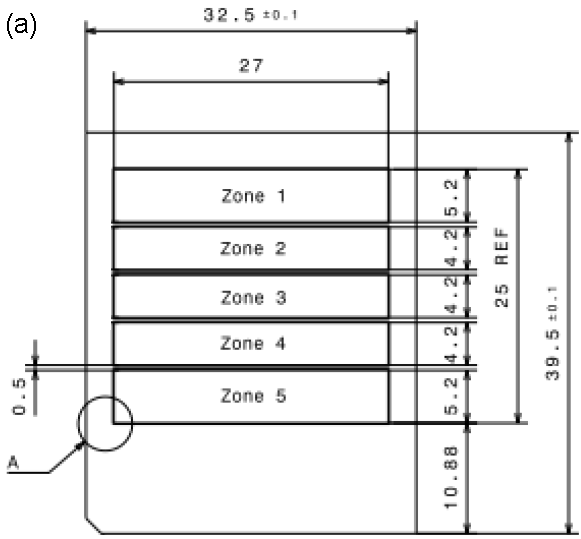
\includegraphics[scale=0.8]{Figs/cuantificaciondefectos/dimsfiltro.png}}{\caption{Dimensiones del filtro especificadas por el fabricante.}\label{fig:dimsfiltr}}
		\ffigbox{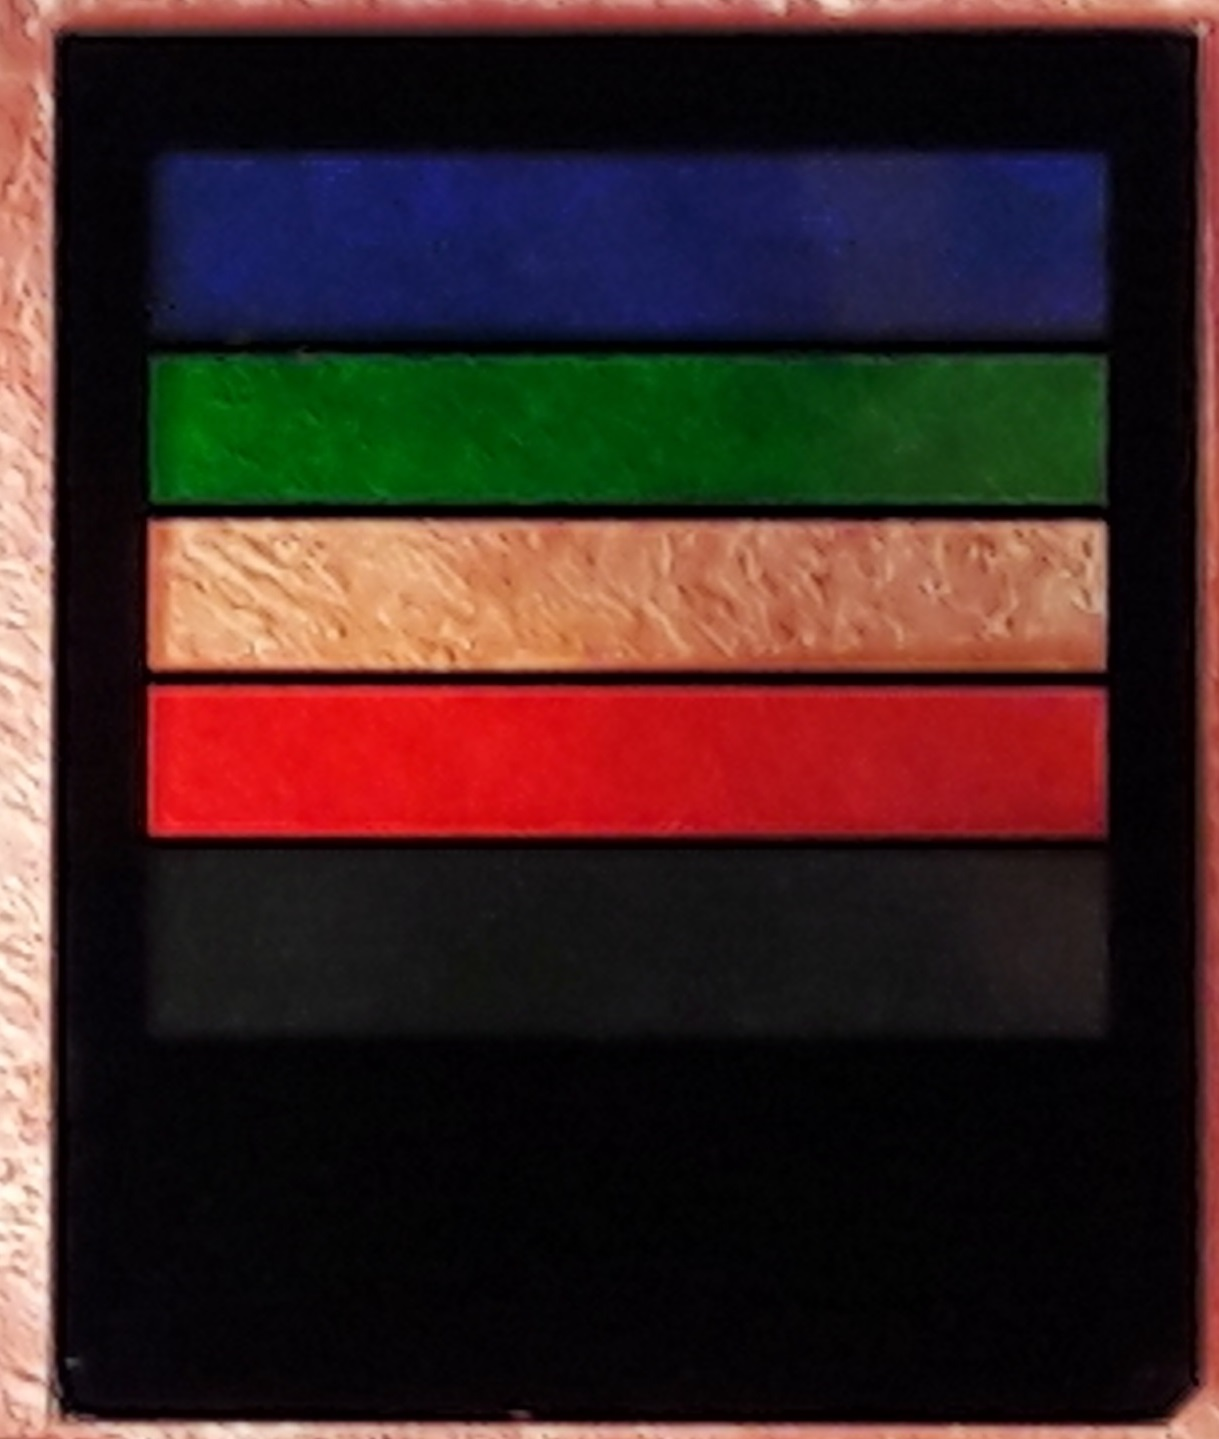
\includegraphics[scale=0.15]{Figs/cuantificaciondefectos/filtro_real.jpg}}{\caption{Imagen del filtro real analizado.}\label{fig:filtroposta}}
	\end{floatrow}
\end{figure}
Las zonas (en inglés, \textit{zone}) están asociadas a una cierta banda espectral de transmisión de la siguiente manera:
\begin{itemize}
\justifying
\item Zona 1 - Banda Azul: (450-510) nm
\item Zona 2 - Banda Verde: (510-580) nm
\item Zona 3 - Banda Pancromática\footnote{La palabra pancromática, del griego ático donde pan significa todo y cromático viene de la familia de la palabra color, implica que dicha banda tiene un espectro de transmisión en toda la región del visible.}: (450-750) nm
\item Zona 4 - Banda Roja: (590-690) nm
\item Zona 5 - Banda NIR: (750-900) nm
\end{itemize}
 \hspace{0.5cm}Las especificaciones ópticas de calidad de cada banda del filtro brindadas por el fabricante fueron las siguientes:
\begin{center}
5/2x0.063 (\textit{S/D 20-10, according to MIL PRF 13830}).
\end{center}
\hspace{0.5cm}Estas especificaciones implican para el caso de la ISO 10110, 5/2x0.063, que en la superficie óptica de cada banda puede haber un máximo de 2 defectos de \textit{grade number} igual a 0.063 (63 $\mu m$ de diámetro), que no puede haber defectos con un \textit{grade number} mayor a 0.063 y que el área total máxima cubierta por defectos de \textit{grade number} mayor ó igual al mínimo valor especificado por el fabricante puede ser de 7938 $\mu m^{2}$, de acuerdo a \ref{eq:isoarea}. Y, las especificaciones de \textit{scratch \& dig}, S/D 20-10, indican que en cada banda puede haber rayaduras con un brillo calibrado de \textit{scratch number} igual 20 y que la suma de todas las longitudes de las rayaduras del mismo valor de \textit{scratch number} no podrá ser superior al diámetro equivalente de cada banda, de acuerdo a \ref{eq:snumb}. Por último, cada banda del filtro no deberá tener más de 1 defecto de \textit{dig number} igual a 10 (diámetro de 100 $\mu m$)  de acuerdo a \ref{eq:nphi20}\footnote{Las dimensiones de la banda más chica son de 4.2 mm x 27.0 mm con lo cual el diámetro equivalente es de aproximadamente 12 mm. El cociente de la Ecuación \ref{eq:nphi20} es igual a 0.6, resultado que se trunca a 1. El resultado final es el mismo para todas las bandas.}  y la suma de los diámetros de todos los defectos no podrá ser superior a los 0.2 mm, de acuerdo a \ref{eq:dmenorig}. 

El fabricante no aclaró el método de inspección utilizado para garantizar la calidad óptica especificada del filtro de la normativa ISO 10110. Ahora bien, como ejercicio de aplicación se va a suponer que el fabricante realizó una inspección visual con muestras calibradas para garantizar la calidad óptica de sus componentes con lo cual en la presente tesis se va a suponer que dicha especificación fue realizada a través de ese método únicamente.

Se hace notar que entre las bandas se encuentran unas regiones rectangulares de un material denominado por el fabricante como cromo negro, de $(0.5 \pm 0.1)mm $ de longitud como se muestra en la Figura \ref{fig:dimsfiltr}. El cromo sirve para aislar espectralmente a cada par de bandas contiguas entre sí del filtro por lo que reduce el potencial \textit{cross-talk}\footnote{El \textit{cross-talk} sería la intromisión del espectro de transmisión de una banda en la detección del espectro de su banda contigua.} en el sensor de imagen. El mismo material cubre toda la región del filtro no contenida por las cinco bandas. 

En esta sección se explicaron las características del filtro y se precisaron las especificaciones ópticas de calidad indicadas por el fabricante. A continuación se describe el proceso de adquisición de las imágenes del filtro, posteriormente su procesamiento y luego el algoritmo de detección de los defectos. A partir de los resultados del algoritmo se pudieron verificar bajo ciertas condiciones los criterios de calidad de las normativas explicadas en la Sección \ref{sec:defectsurf} y establecer los criterios de diseño del microespectrómetro construido que se explica en el Capítulo \ref{chap:microsp}.

%%%%%%%%%%%%%%%%%%%%%%%%%%%%%%%%%%%%%%%%%%%%%%%%%%%%%%%%%%%%%%%%%%%%%%%%%%%%%%%%%%%%%%%%%%%%%%%%%%%%%%%%%%%%%%%%%%%%%%%%%%%%%%%%%%%%%%%%%%%%%%%%%%%%%%%%%%%%%%%%%%%%%%%%%%%%%%%%%%%%%%%%%%%%%%%%%%%%%%%%%%%%%%%%%%%%%%%%%%%%
\singlespacing
\section{Adquisición de las imágenes del filtro}
\label{sec:conf}
\spacing{1.5}

\hspace{0.5cm}Con el propósito de cuantificar y caracterizar los defectos del filtro se adquirieron imágenes micróscopicas del mismo. Para la adquisición de las imágenes se utilizó un microscopio invertido Zeiss Axio Observer Z1 como se muestra en la Figura \ref{fig:ZEISSdellabo}, con un objetivo Zeiss N-Achroplan de magnificación 10X y apertura numérica de 0.25.
\begin{figure}[H]
	\centering
	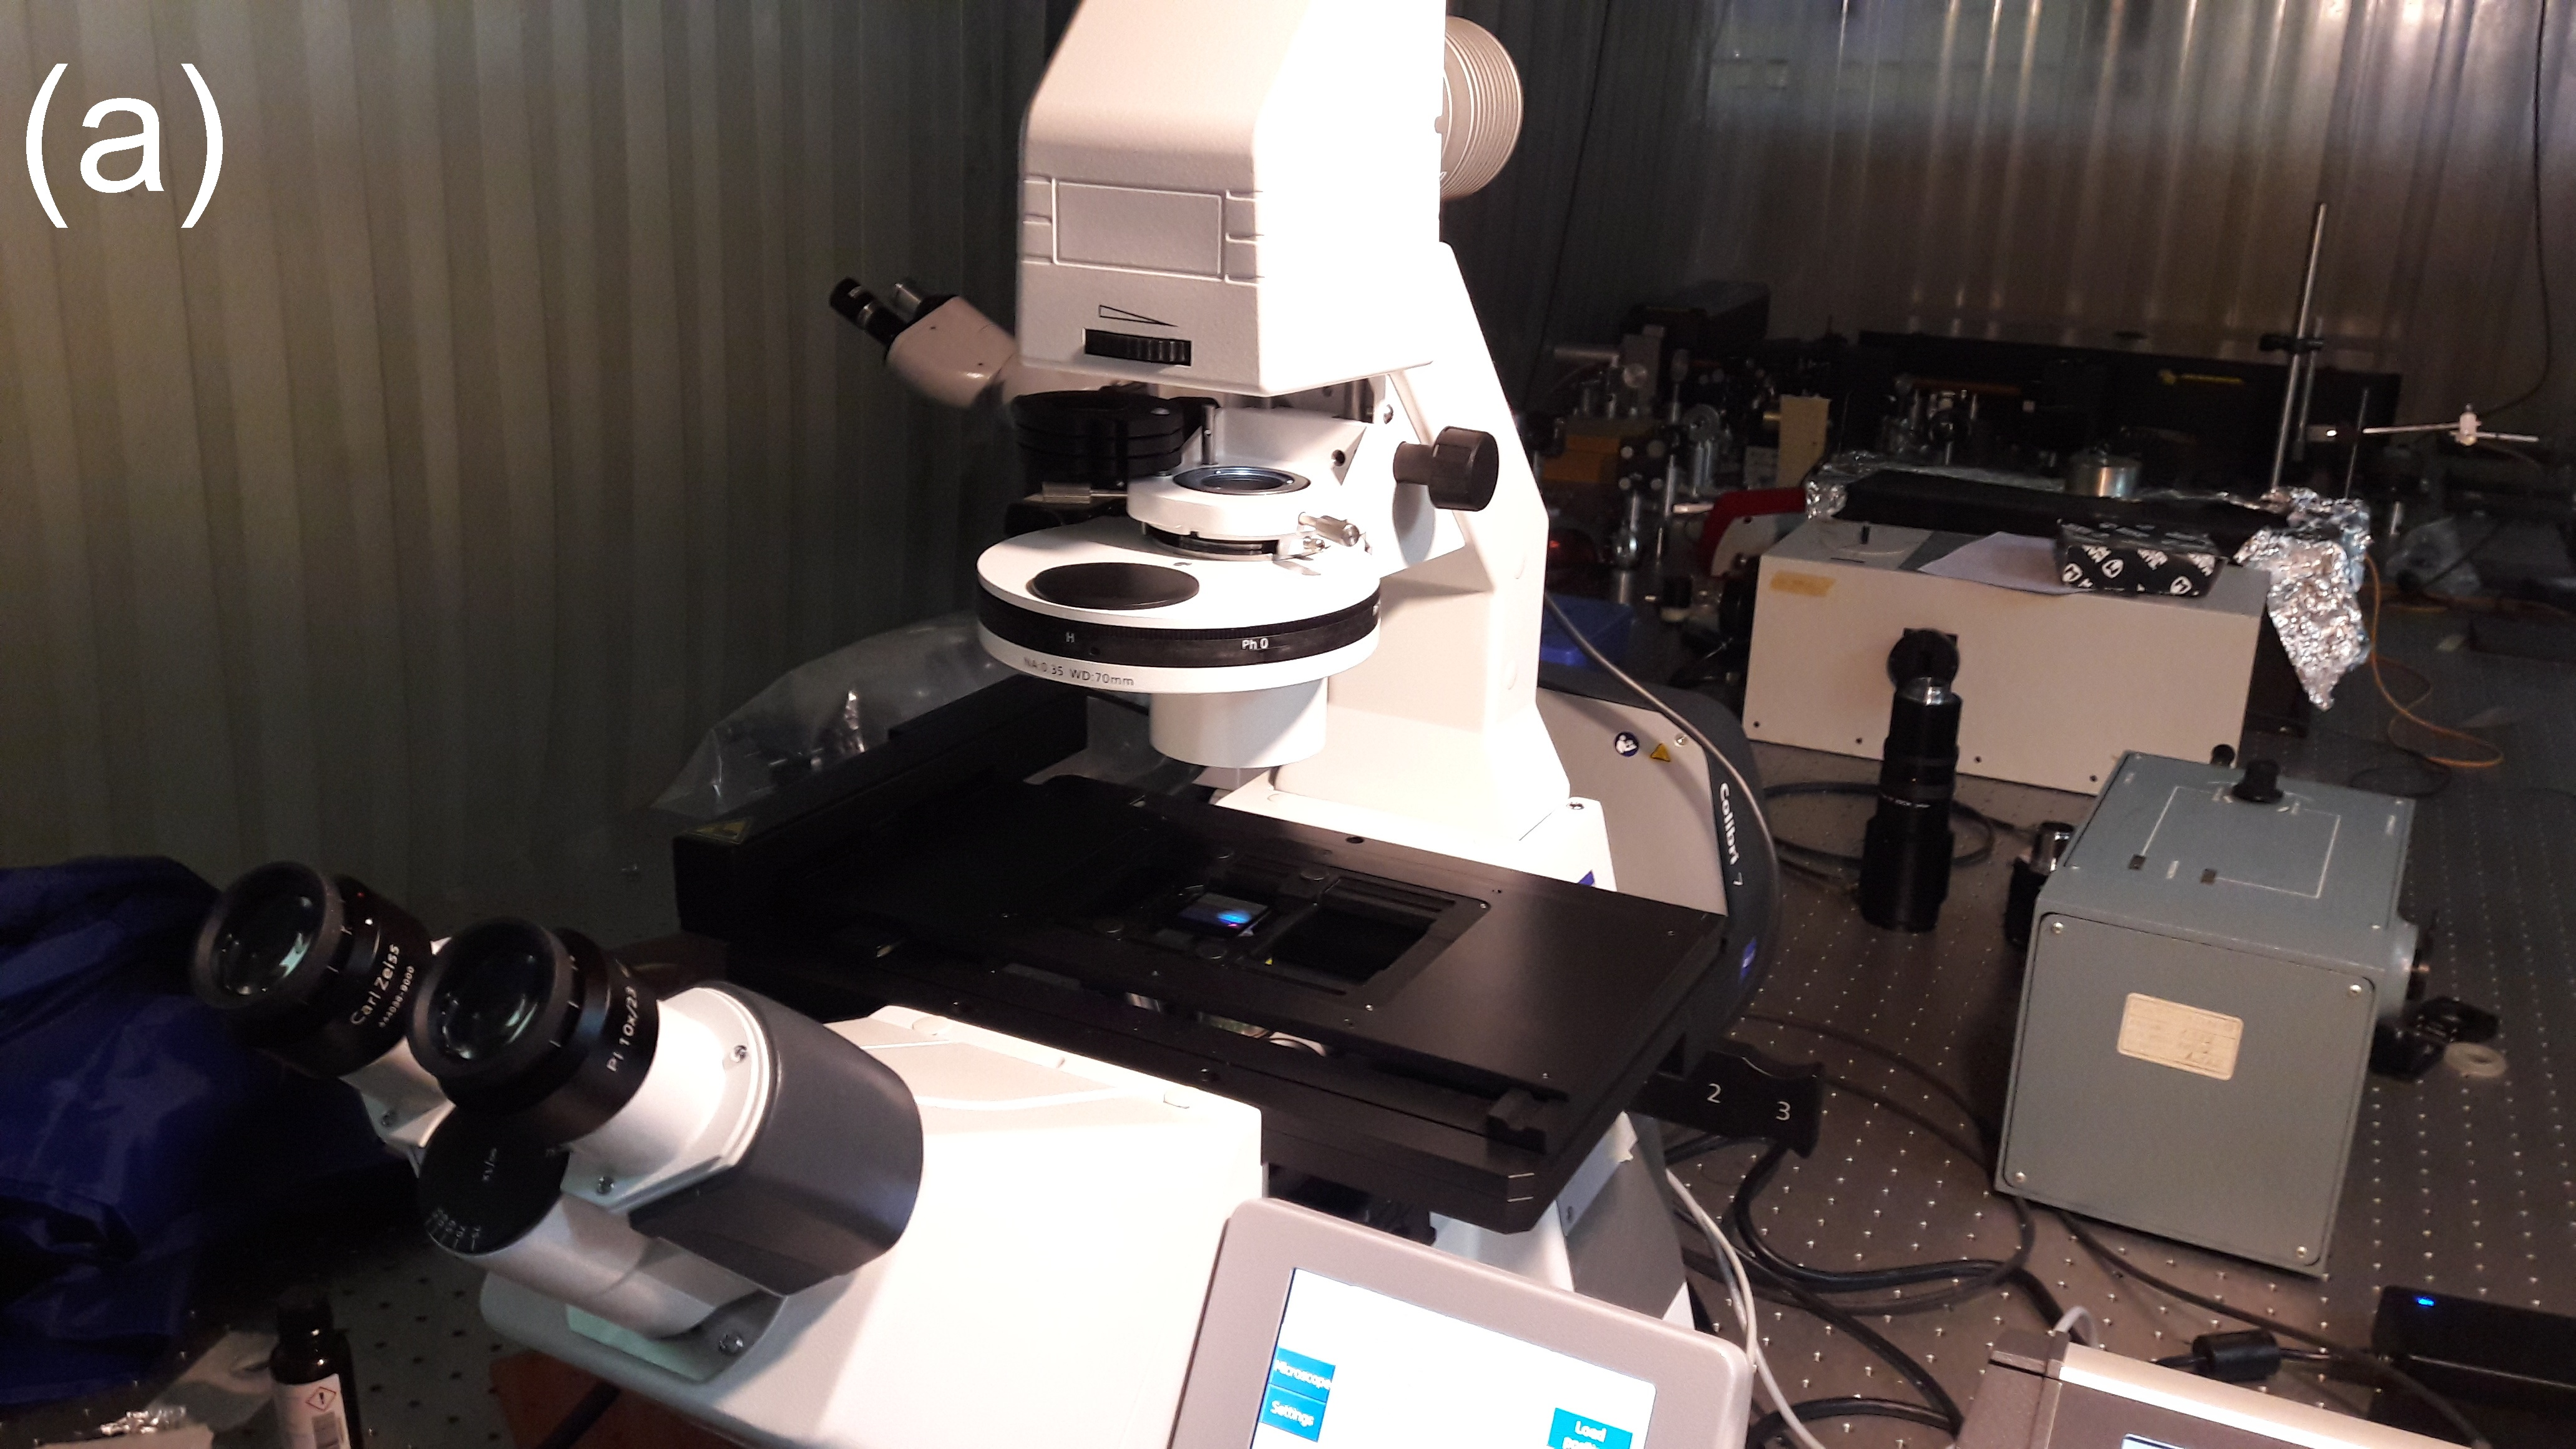
\includegraphics[scale=0.1]{Figs/defectosZEISS/b.jpg}
	\caption{Microscopio invertido Zeiss Axio Observer Z1.}
	\label{fig:ZEISSdellabo}
\end{figure}

Las imágenes del filtro fueron adquiridas por transmisión utilizando una fuente de luz blanca, en condiciones de \textit{bright field}\footnote{Técnica de iluminación que en castellano suele ser denominada de 'campo brillante' para diferenciarla de la iluminación de campo oscuro (en inglés \textit{dark field}, ver \href{https://es.wikipedia.org/wiki/Microscopio_de_campo_oscuro}{\faWikipediaW}).}.  
\begin{figure}[H]
	\centering
	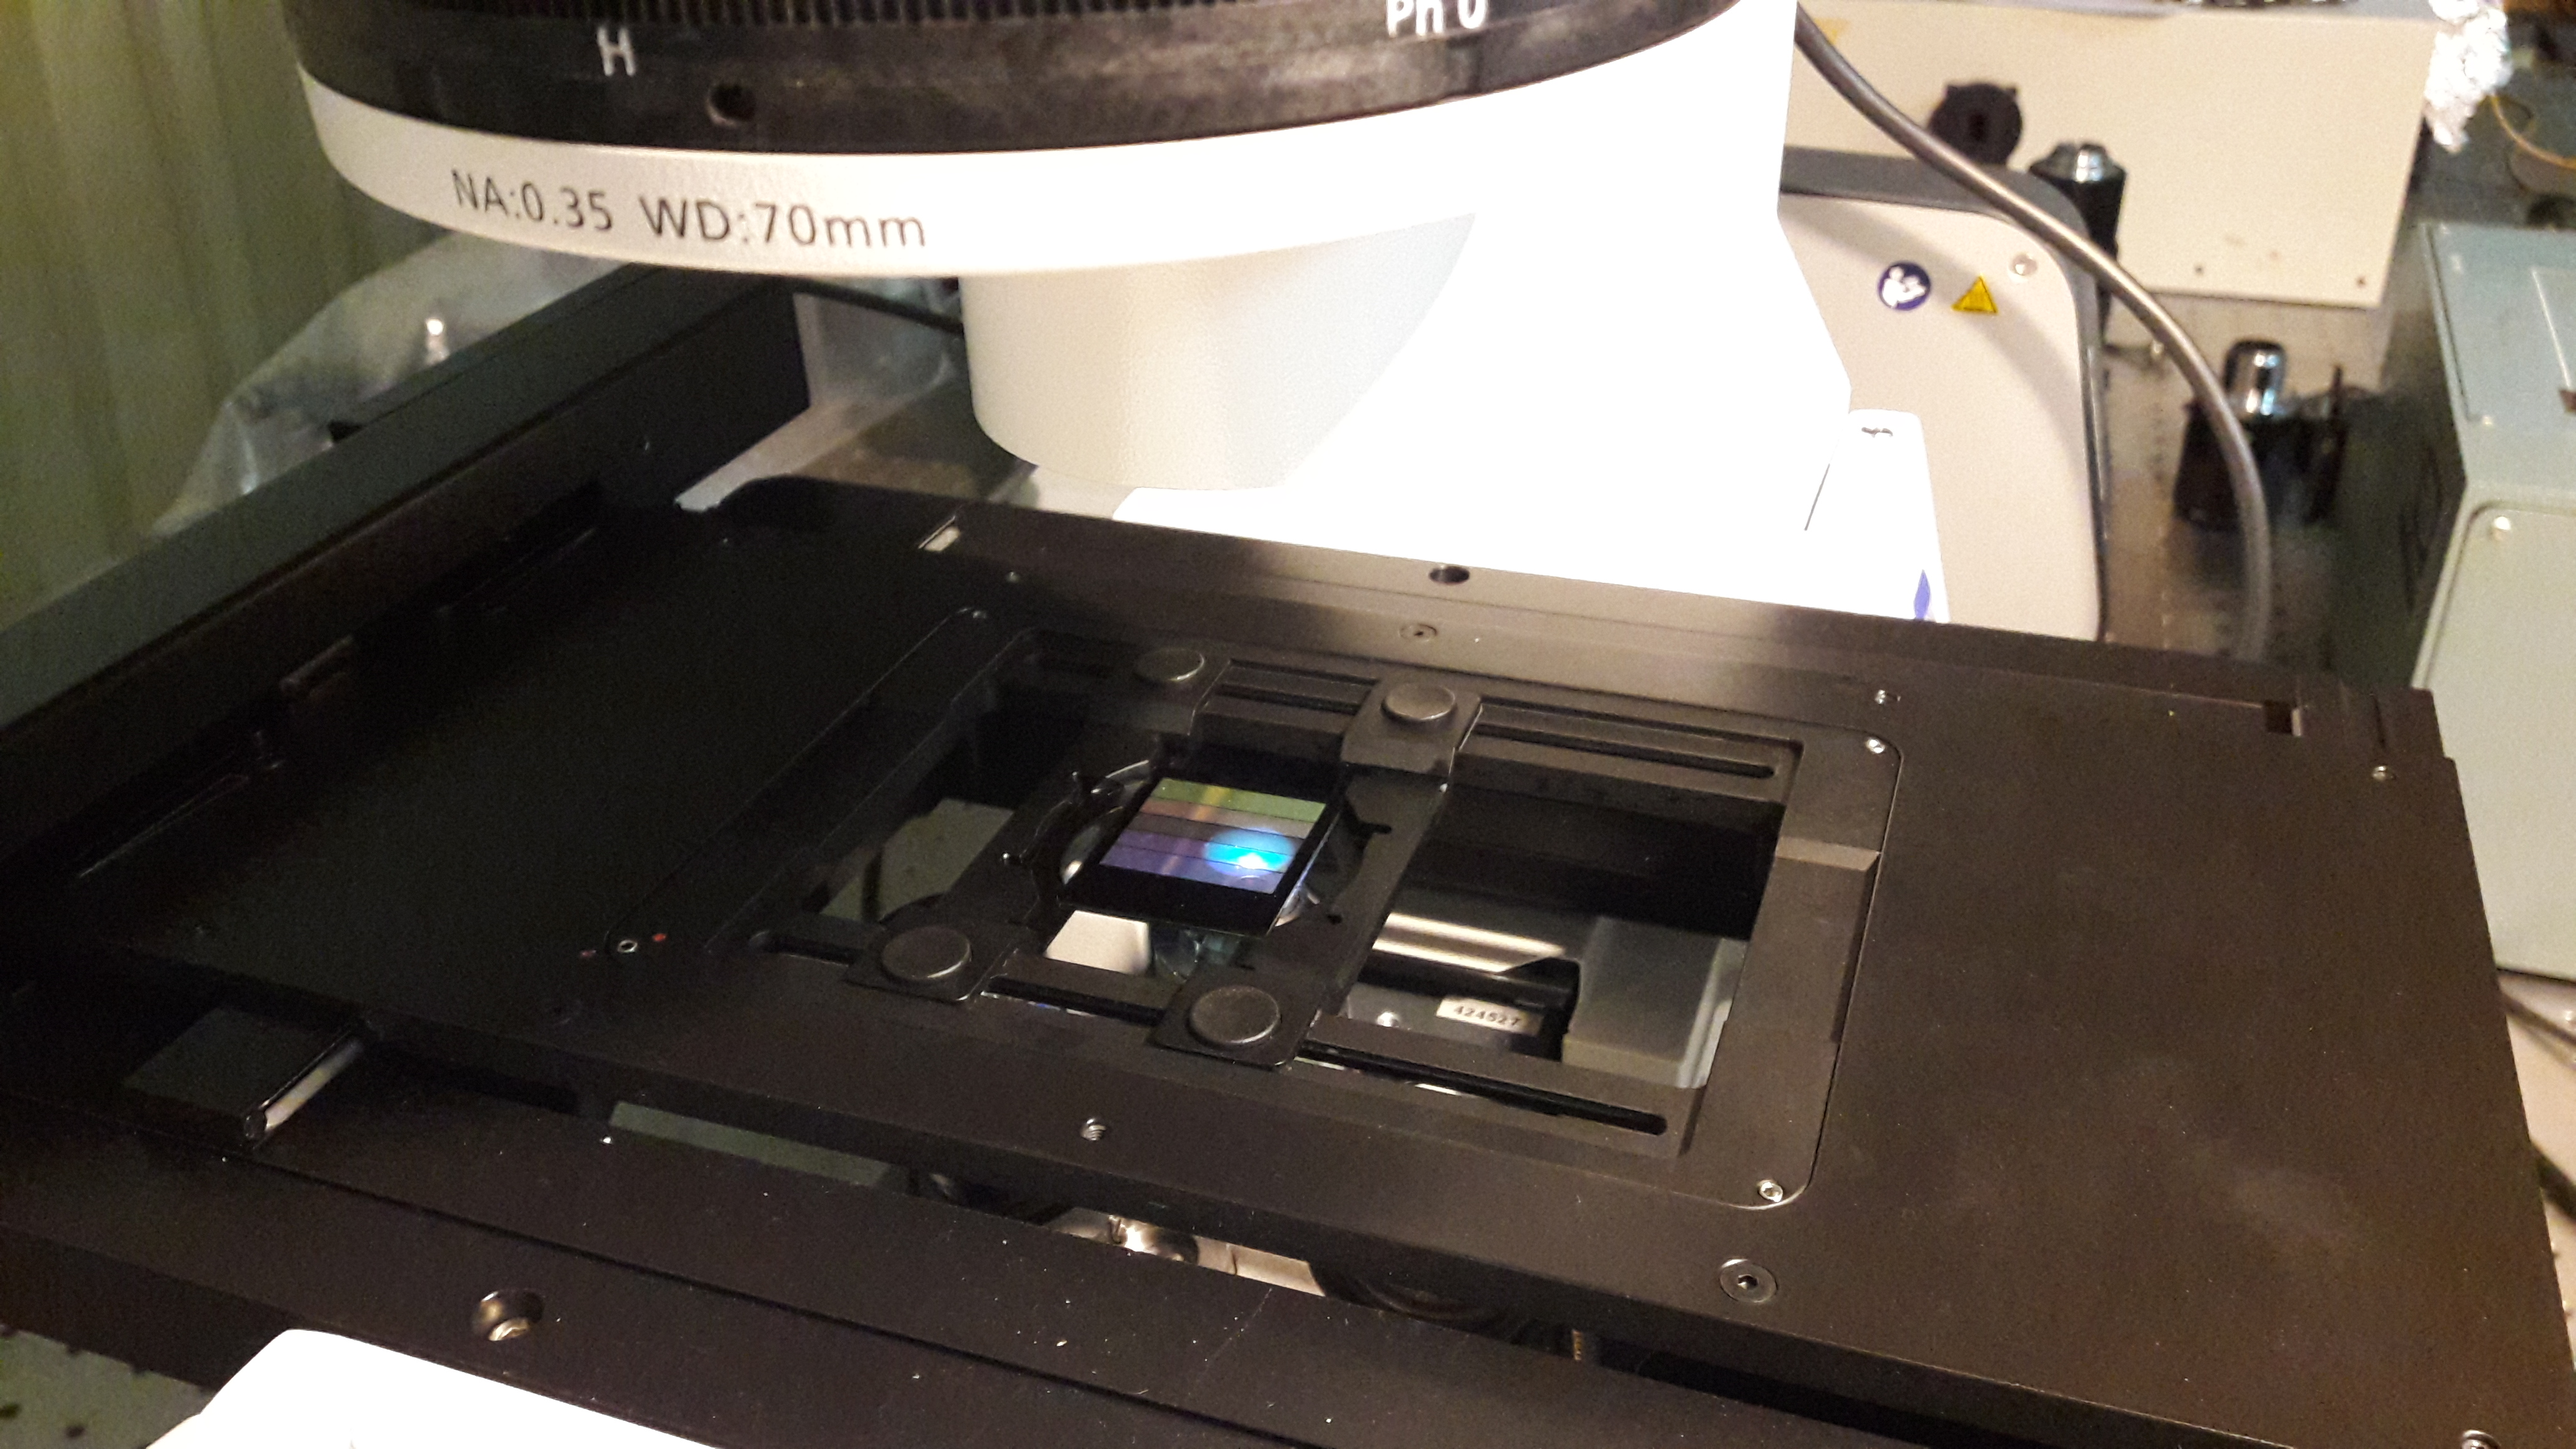
\includegraphics[scale=0.1]{Figs/defectosZEISS/a.jpg}
	\caption{Montaje del filtro sobre el portamuestras de la platina del microscopio.}
	\label{fig:filtroenZEISS}
\end{figure}
La cámara monocromática del microscopio del fabricante Zeiss, modelo Axiocam 702, con un sensor CMOS de 1/1.2'' (diagonal de 13.3mm) y una resolución de 2.3 megapíxeles (1216x1920 píxeles), fue controlada a través del software ZEN 2.5 (\textit{Blue edition}, 2018) del mismo fabricante. Se utilizó la calibración de la cámara que viene de fábrica del microscopio para la configuración utilizada, donde 1 píxel equivale a 0.586 $\mu m$.  Cada imagen individual tiene las dimensiones del \textit{field of view} (FOV\footnote{En castellano es el campo de visión y representa el área física de la imagen, que para el caso de una cámara el FOV viene dado por el cociente entre el tamaño del sensor CMOS y la magnificación del microscopio.}) de la cámara, que son de 713 $\mu m$ x 1125 $\mu m$. 

Se configuró el software para adquirir las imágenes por transmisión, en particular se eligió la fuente de luz blanca y para cada medición su intensidad, además del tiempo de exposición de la cámara. Se montó el filtro sobre el portamuestras de la platina del microscopio como se muestra en la Figura \ref{fig:filtroenZEISS} y con las perillas manuales del microscopio se puso en foco la imagen observando la adquisición en vivo en la computadora. 

%%%%%%%%%%%%%%%%%%%%%%%%%%%%%%%%%%%%%%%%%%%%%%%%%%%%%%%%%%%%%%%%%%%%%%%%%%%%%%%%%%%%%%%%%%%%%%%%%%%%%%%%%%%%%%%%%%%%%%%%%%%%%%%%%%%%%%%%%%%%%%%%%%%%%%%%%%%%%%%%%%%%%%%%%%%%%%%%%%%%%%%%%%%%%%%%%%%%%%%%%%%%%%%%%%%%%%%%%%%%

\singlespacing
\subsection{\textit{Tile scan}}
\label{subs:tilsc}
\spacing{1.5}

\hspace{0.5cm}A continuación se explica cómo se adquirieron las imágenes para una determinada región del filtro, ya sea para el filtro completo a excepción de la banda del NIR ó para cada banda espectral del filtro en particular.

La palabra en inglés \textit{tile} significa baldosa en castellano y realizar un \textit{tile scan} implica realizar un barrido de adquisición de imágenes de una cierta área a elección de una muestra donde el área total a adquirir está compuesta por múltiples baldosas. Cada baldosa, es decir cada \textit{tile} constituye una imagen del microscopio de acuerdo al \textit{field of view} (FOV) que se tiene del arreglo óptico de la cámara integrada al microscopio. En la Figura \ref{fig:tilescan} se muestra un ejemplo de un \textit{tile scan} de la banda pancromática del filtro.

Existen distintas formas de elegir el área total a adquirir en el software. Se eligió la opción de determinar la región a adquirir a partir de la selección visual individual de las cuatro esquinas de la misma, es decir las posiciones [0,0],[xf,0],[0,yf], [xf,yf] de acuerdo al sistema de coordenadas de la Figura \ref{fig:tilescan}. Para elegir estas esquinas el microscopio cuenta con un \textit{joystick} que permite mover la platina motorizada del microscopio en el plano de la imagen y se tiene activada la adquisición en vivo en el software ZEN para elegirlas visualmente.


\begin{figure}[H]
	\centering
	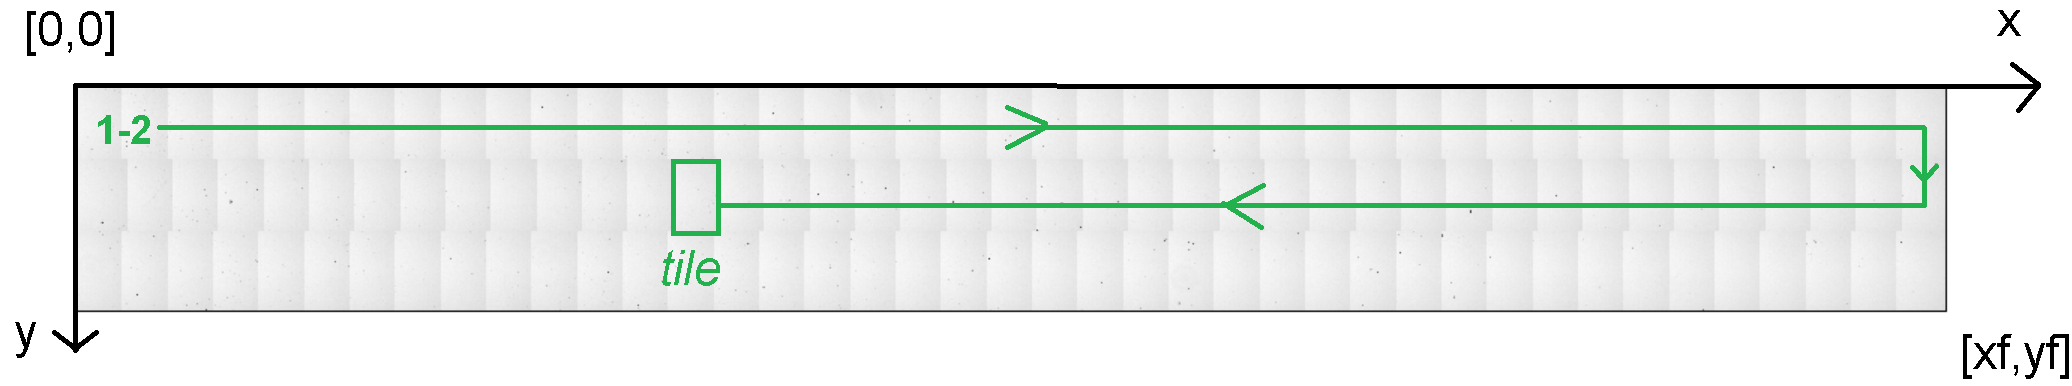
\includegraphics[width=1.0\textwidth]{Figs/cuantificaciondefectos/tilescan.png}
	\caption{\textit{Tile scan} de la banda pancromática.}
	\label{fig:tilescan}
\end{figure} 

Cada trayectoria del barrido fue realizada automáticamente de la siguiente manera: la platina motorizada se posicionó en el centro del FOV de la primera \textit{tile} a adquirir asociada a las coordenadas [0,0] de la imagen de la Figura \ref{fig:tilescan} y se adquirió la primera imagen individual del barrido completo de la región a adquirir, en este ejemplo la banda pancromática. A continuación la platina motorizada se desplazó en el sentido definido positivo del eje $x$ hasta el centro del FOV de la segunda \textit{tile} a adquirir teniendo en cuenta el \textit{overlap} configurado y así siguiendo una trayectoria que barre por `filas' completas a lo largo del eje $\textit{x}$ que van variando con el desplazamiento discreto vertical en el eje $\textit{y}$ cuando se llega a los extremos del eje $\textit{x}$.

Entre otros parámetros del barrido, se eligió el \textit{overlap} entre las baldosas, es decir la superposición entre las mismas que luego permite obtener una imagen completa individual para su visualización,  realizando un \textit{stitching}\footnote{El \textit{stitching} es el proceso computacional por el cual se combinan múltiples \textit{tiles} para
producir una sola imagen que permita una mejor visualización (Ver técnica SIFT (\textit{Scale Invariant Feature Transform}), \cite{Lowe}).} como post-procesamiento de las imágenes. Este último procedimiento también fue realizado con el software de Zeiss. Por último, se elige en la configuración que cada baldosa de la región barrida sea exportada como una imagen individual para su posterior análisis.

%%%%%%%%%%%%%%%%%%%%%%%%%%%%%%%%%%%%%%%%%%%%%%%%%%%%%%%%%%%%%%%%%%%%%%%%%%%%%%%%%%%%%%%%%%%%%%%%%%%%%%%%%%%%%%%%%%%%%%%%%%%%%%%%%%%%%%%%%%%%%%%%%%%%%%%%%%%%%%%%%%%%%%%%%%%%%%%%%%%%%%%%%%%%%%%%%%%%%%%%%%%%%%%%%%%%%%%%%%%%
\singlespacing
\subsection{Superficies y mapa de los defectos del filtro}
\label{subs:compl}
\spacing{1.5}

\hspace{0.5cm}Se adquirieron imágenes completas del filtro, para las dos superficies exteriores del filtro como se muestra en las Figuras \ref{fig:supfiltrocondensador} y \ref{fig:supfiltroobjetivo}.
\begin{figure}[H]
	\begin{floatrow}
		\ffigbox{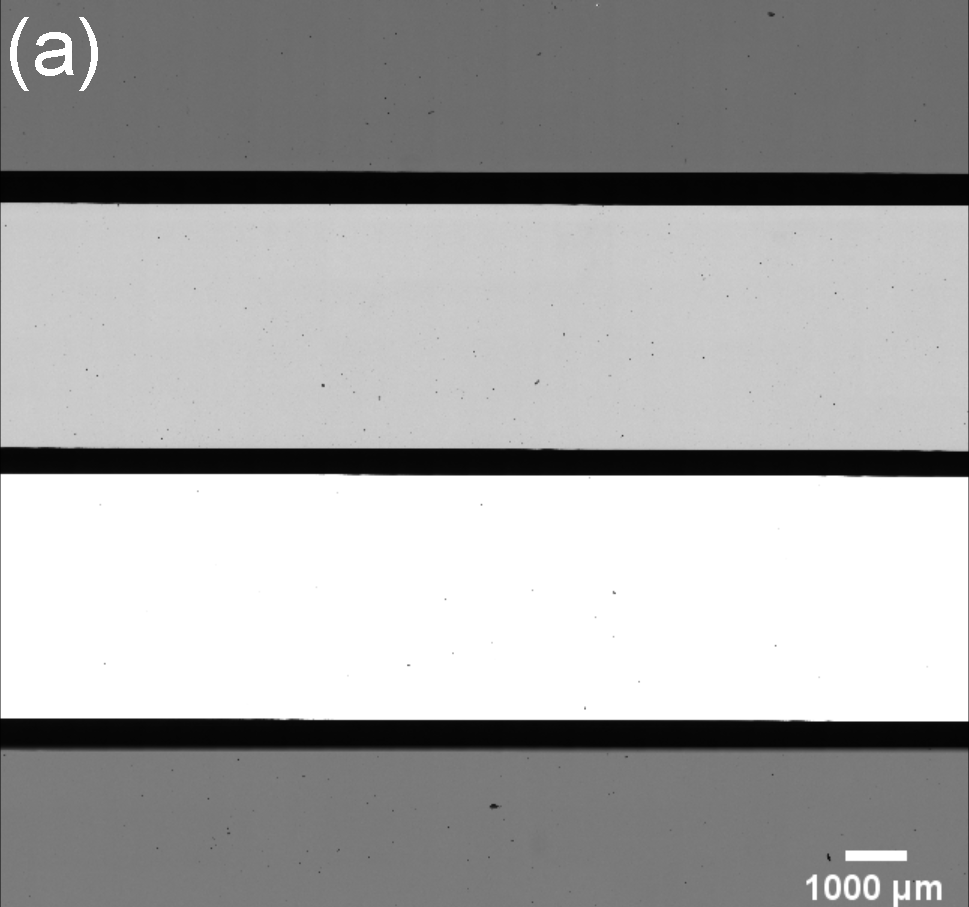
\includegraphics[width=7.5cm,height=7.33cm]{Figs/cuantificaciondefectos/supextex2216.png}}{\caption{Imagen de la superficie exterior A del filtro, resultado del \textit{stitching} de las imágenes de un barrido de 15.54 mm x 14.94 mm. El \textit{overlap} configurado entre las \textit{tiles} fue de 30\%.}\label{fig:supfiltrocondensador}}
		\ffigbox{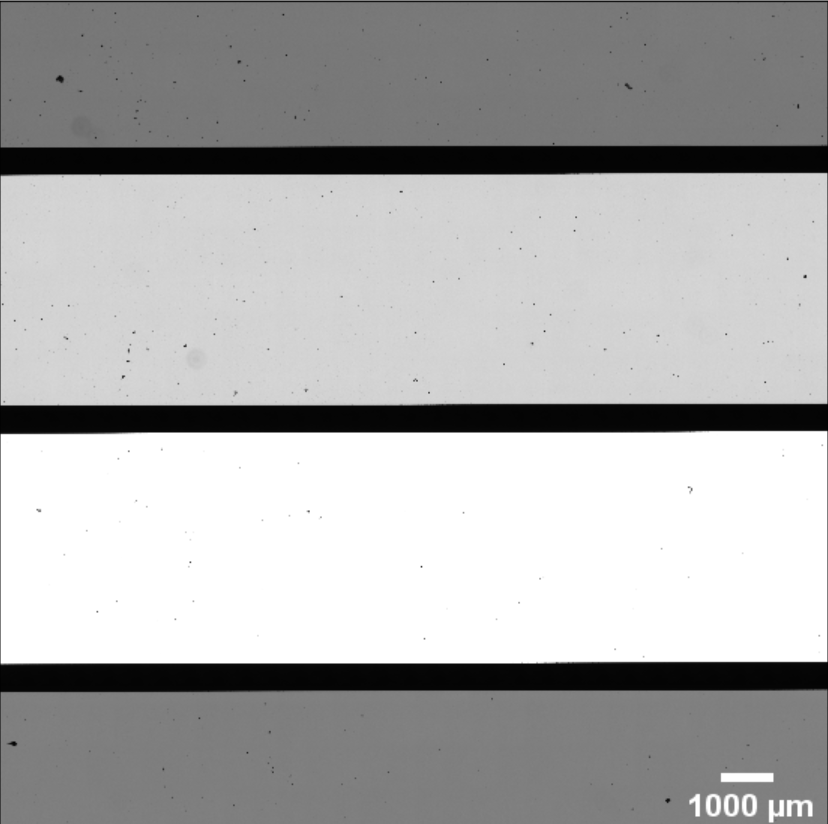
\includegraphics[width=7.5cm,height=7.33cm]{Figs/cuantificaciondefectos/supextex1515.png}}{\caption{Imagen de la superficie exterior B del filtro, resultado del \textit{stitching} de las imágenes de un barrido de 15.50 mm x 15.55 mm. El \textit{overlap} configurado entre las \textit{tiles} fue de 30\%.}\label{fig:supfiltroobjetivo}}
	\end{floatrow}
\end{figure}
 Las dos superficies exteriores denominadas arbitrariamente A y B son las que se muestran especificadas en la Figura \ref{fig:espfil} y que se encuentran en la interfaz filtro-aire. En las Figuras \ref{fig:supfiltrocondensador} y \ref{fig:supfiltroobjetivo} se muestran las bandas espectrales del filtro en orden descendente: Azul (450-510 nm), Verde (510-580 nm), Pancromática (450-750 nm), Roja (590-690 nm). El brillo, el contraste y el tamaño de las imágenes originales fueron modificados para obtener una mejor visualización, utilizando el software FIJI-ImageJ. 
\begin{figure}[H]
	\centering
	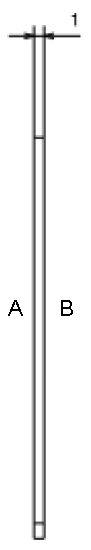
\includegraphics[scale=0.4]{Figs/cuantificaciondefectos/espesorfiltro.png}
	\caption{Dimensiones del espesor del filtro: (1.0 $\pm$ 0.1)mm. Las superficies exteriores del filtro son las superficies A y B, que se encuentran en la interfaz filtro-aire.}
	\label{fig:espfil}
\end{figure}
Para realizar el barrido completo de cada superficie se verificó en las cuatro esquinas de la superficie a medir que no se pierda el foco de la imagen. Se eligió la intensidad de la fuente de luz y el tiempo de integración de la cámara tales que no sature alguna de las bandas del filtro de forma tal poder adquirir una imagen completa del filtro en un solo barrido, y de forma tal que se utilice la mayor parte del rango dinámico de la cámara, como se puede ver en el histograma de la intensidad de los píxeles de la Figura \ref{fig:histograma15x15} para el barrido de la superficie A del filtro. 
\begin{figure}[H]
	\centering
	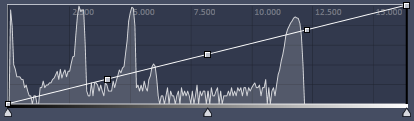
\includegraphics[width=1.0\textwidth]{Figs/defectosZEISS/histograma15x15.png}
	\caption{Histograma de la intensidad de los píxeles de la cámara del barrido de la superficie exterior A del filtro que se observa en el software ZEN del microscopio.}
	\label{fig:histograma15x15}
\end{figure}
Se hace notar que la banda del NIR no pudo ser adquirida en el barrido completo de las superficies exteriores del filtro pues con los valores de intensidad de la lámpara y del tiempo de adquisición de la cámara fijados para que ninguna de las bandas del filtro sature, no era posible obtener una imagen de esa banda. Si bien la cámara tiene un rango de sensibilidad espectral comprendido entre los 350 nm y los 1000 nm de acuerdo a su hoja de datos \cite{axiozeiss}, del gráfico de la eficiencia cuántica\footnote{La eficiencia cuántica, en inglés \textit{Quantum efficiency} (QE), es una medida precisa de la sensibilidad de un dispositivo fotosensible que permite determinar como es la respuesta del dispositivo para cada longitud de onda.} se desprende que para la región espectral del NIR tiene una eficiencia cuántica menor al 30\% (Ver Figura \ref{fig:eficienciacuanticamara}). A esto se le suma el hecho de que la fuente de luz tiene un espectro de emisión centrada en el ultravioleta y con una fuerte componente del espectro visible pero de muy baja intensidad en la región del NIR, como se muestra en el gráfico de la intensidad en función de la longitud de onda de la Figura \ref{fig:espectrolamparazeiss}. Dicho espectro fue medido con el espectrómetro CCS200 de Thorlabs y se hace notar que dicha fuente de luz es utilizada con muestras biológicas. Ahora bien, la banda espectral del NIR fue medida individualmente posteriormente como se muestra en la Sección \ref{sec:cadab}.

\begin{figure}[H]
	\centering
	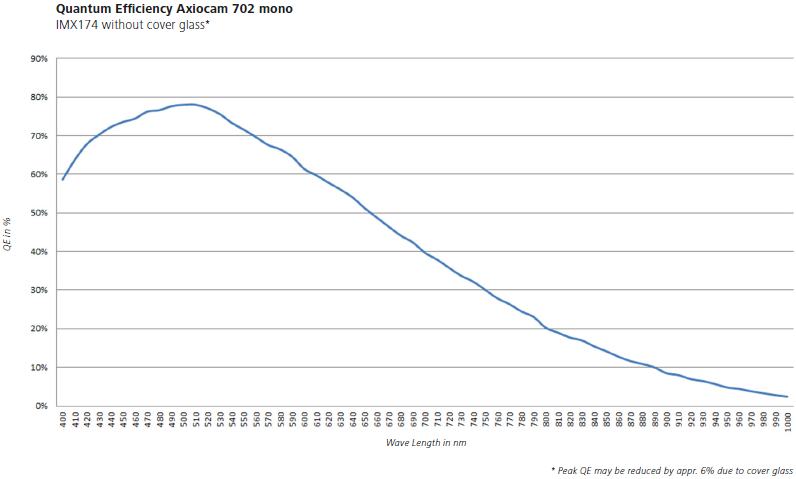
\includegraphics[width=1.0\textwidth]{Figs/defectosZEISS/eficienciacuanticacamarazeiss.png}
	\caption{Gráfico de la eficiencia cuántica de la cámara monocromática del microscopio Aiocam 702 en función de la longitud de onda.}
	\label{fig:eficienciacuanticamara}
\end{figure}
Como criterio de diseño y construcción de un equipo de microscopía para inspeccionar los filtros como el analizado en el presente trabajo, se debería considerar para la adquisición de la banda del NIR una fuente de luz infrarroja y una cámara con una respuesta espectral específica de dicha región del espectro. Y, para el resto de las bandas se podría utilizar una fuente de luz de banda ancha en la región del espectro visible como la que se utilizó en el montaje del equipo desarrollado que se explica en el Capítulo \ref{chap:microsp}. Más aún, queda pendiente como trabajo a futuro la aplicación de otras técnicas de microscopía como \textit{Dark Field Microscopy} ó \textit{Differential Interference Contrast Microscopy} (DIC).
\begin{figure}[H]
	\centering
	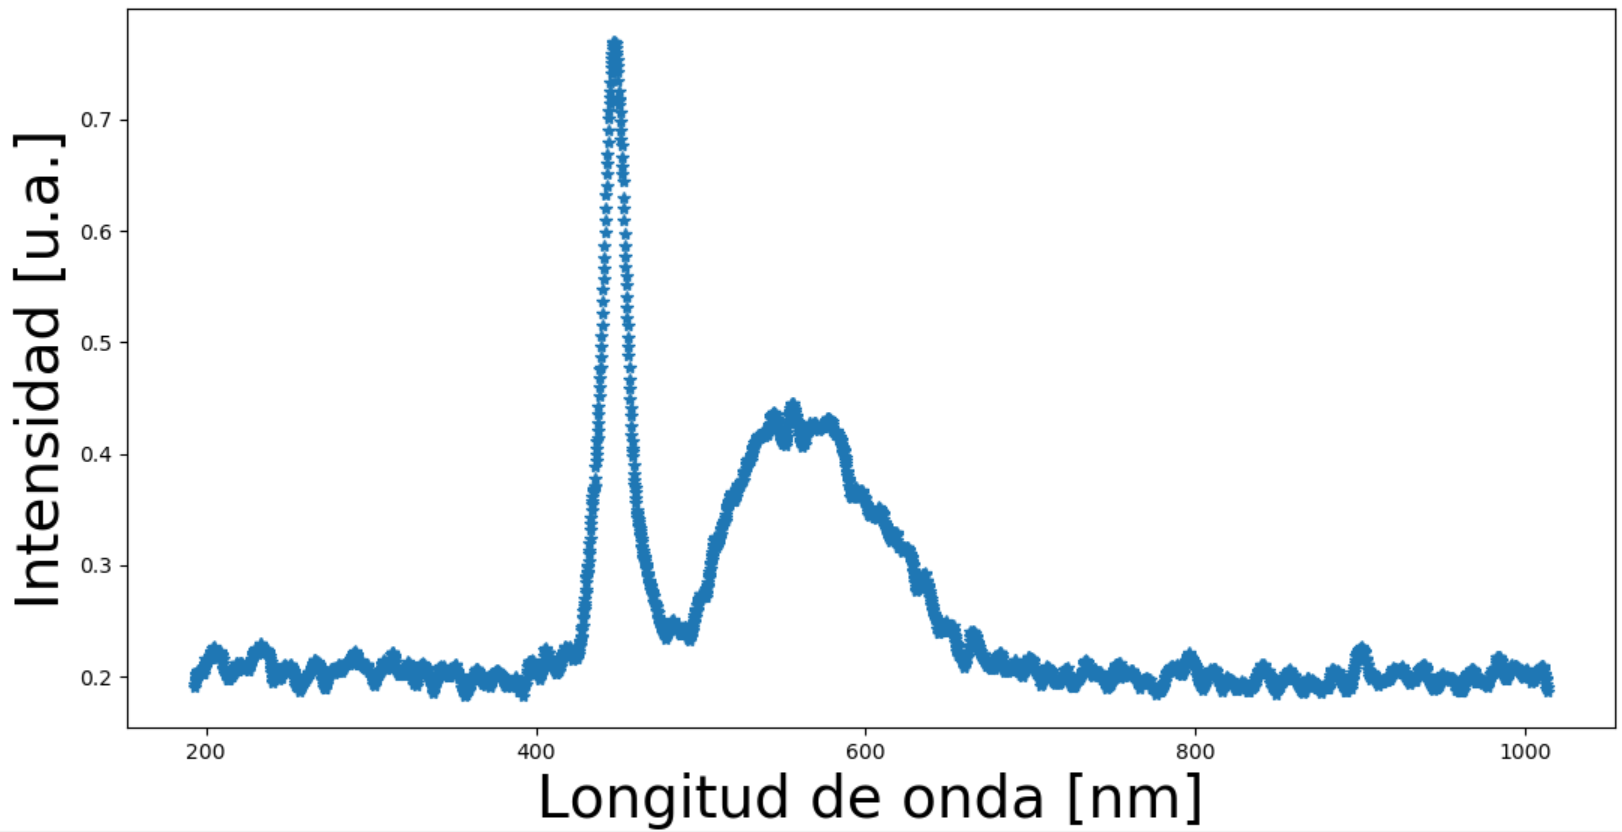
\includegraphics[width=1.0\textwidth]{Figs/defectosZEISS/espectrolampZEISS.png}
	\caption{Espectro de emisión de la fuente de luz del microscopio.}
	\label{fig:espectrolamparazeiss}
\end{figure}

La imagen completa de cada superficie exterior del filtro permitió realizar un primer diagnóstico visual general por imagen de la calidad óptica de construcción del filtro. Además, permitió obtener un mapa de los defectos con su ubicación precisa en la superficie del filtro para ser utilizado luego con el microespectrómetro (Ver Capítulo \ref{chap:microsp}). Por último, se midió la longitud del cromo que separa las bandas con el software Fiji para realizar la calibración de la platina que se explica en la Sección \ref{sec:platina}.

A continuación se explica el proceso de adquisición de las imágenes individuales de cada banda espectral, el pre-procesamiento de las mismas que consiste en la corrección de la iluminación no uniforme del microscopio y luego se describe el algoritmo de detección de los defectos.

%%%%%%%%%%%%%%%%%%%%%%%%%%%%%%%%%%%%%%%%%%%%%%%%%%%%%%%%%%%%%%%%%%%%%%%%%%%%%%%%%%%%%%%%%%%%%%%%%%%%%%%%%%%%%%%%%%%%%%%%%%%%%%%%%%%%%%%%%%%%%%%%%%%%%%%%%%%%%%%%%%%%%%%%%%%%%%%%%%%%%%%%%%%%%%%%%%%%%%%%%%%%%%%%%%%%%%%%%%%%
\singlespacing
\subsection{Adquisición de imágenes individuales de cada banda espectral}
\label{sec:cadab}
\spacing{1.5}

\hspace{0.5cm}Para realizar la cuantificación de los defectos del filtro, se adquirieron imágenes individuales de cada banda espectral para una de las superficies exteriores del filtro. Para cada banda, se configuró la intensidad de la lámpara y el tiempo de integración de la cámara de forma tal de utilizar la mayor parte del rango dinámico de la cámara que se encuentra alrededor del 70 \% recomendado por el fabricante y de esta forma obtener la mejor calidad de imagen para el posterior análisis de cada banda. Así también se verificó que las cuatro esquinas de la banda a medir estuvieran en foco a partir de la visualización en vivo de la cámara. Dichas esquinas fueron elegidas en el software para determinar el área a ser barrida con el \textit{tile scan} teniendo cuidado de no incluir parte del cromo en el campo de visión de la imagen. Esto resultó importante pues de lo contrario el algoritmo de detección de los defectos detectaba al cromo como un centenar de defectos, que serían falsos positivos\footnote{En el contexto de esta tesis, un falso positivo consistiría en la detección errónea mediante un algoritmo de procesamiento de imágenes de un defecto que en realidad no lo es.}, lo que arruinaría claramente cualquier tipo de análisis cuantitativo. En las Figuras \ref{fig:tilebandaazul}, \ref{fig:tilebandaverde}, \ref{fig:tilebandapanc}, \ref{fig:tilebandaroja} y \ref{fig:tilebandanir} se muestran los \textit{tile scan} de cada banda y en sus epígrafes se detallan los parámetros de cada adquisición. No se realizó un \textit{stitching} de las imágenes de cada banda, ya que se analizaron las imágenes individuales (Ver Sección \ref{sec:preproc}). El \textit{overlap} configurado entre las \textit{tiles} de cada banda fue de 10\%.
\begin{figure}[H]
	\centering
	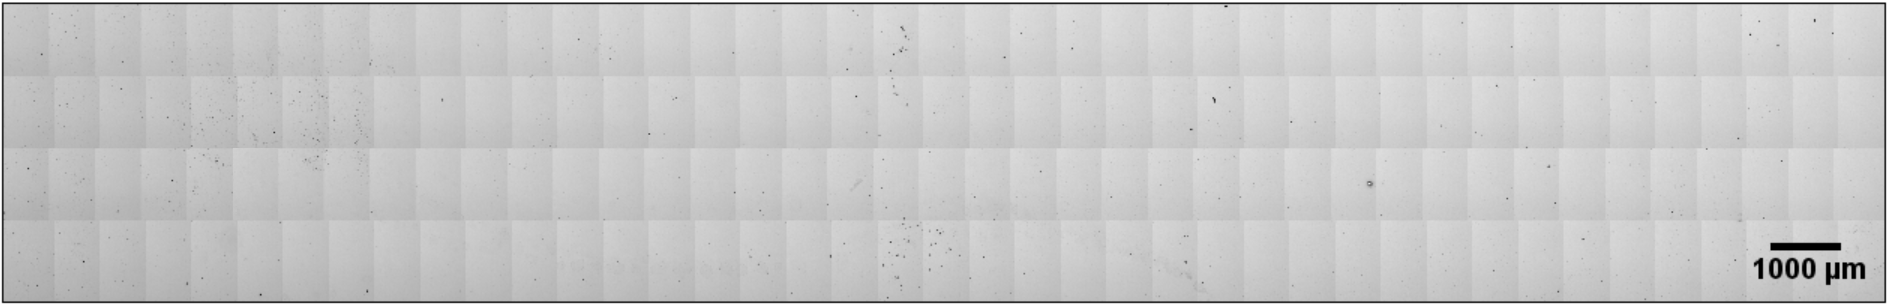
\includegraphics[width=1.0\textwidth]{Figs/cuantificaciondefectos/banda_AZUL.png}
	\caption{Imagen de la banda azul del filtro obtenida mediante un \textit{Tile scan} de 26.37 mm x 4.16 mm, compuesta por 164 \textit{tiles}, con la intensidad de la lámpara configurada en 30\% y el tiempo de exposición de la cámara fue de 40 ms.}
	\label{fig:tilebandaazul}
\end{figure}
\begin{figure}[H]
	\centering
	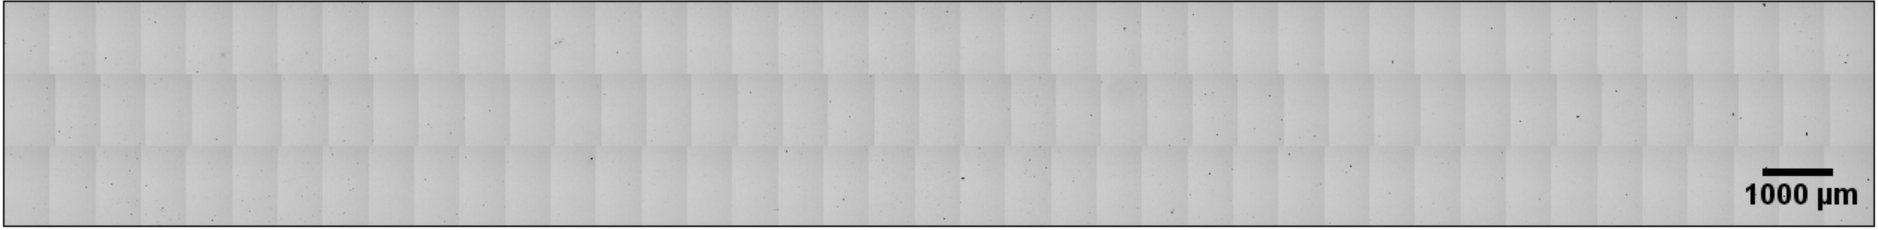
\includegraphics[width=1.0\textwidth]{Figs/cuantificaciondefectos/banda_VERDE.png}
	\caption{Imagen de la banda verde del filtro obtenida mediante un \textit{Tile scan} de 26.37 mm x 3.15 mm, compuesta por 123 \textit{tiles}, con la intensidad de la lámpara configurada en 17\% y el tiempo de exposición de la cámara fue de 40 ms.}
	\label{fig:tilebandaverde}
\end{figure}
\begin{figure}[H]
	\centering
	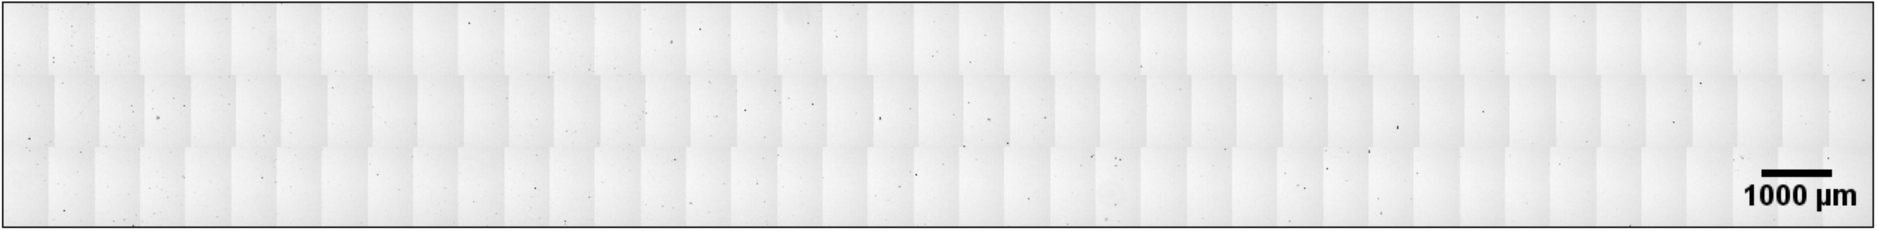
\includegraphics[width=1.0\textwidth]{Figs/cuantificaciondefectos/banda_PANC.png}
	\caption{Imagen de la banda roja del filtro obtenida mediante un \textit{Tile scan} de 26.37 mm x 3.15 mm, compuesta por 123 \textit{tiles}, con la intensidad de la lámpara configurada en 10\% y el tiempo de exposición de la cámara fue de 40 ms.}
	\label{fig:tilebandapanc}
\end{figure}
\begin{figure}[H]
	\centering
	
\includegraphics[width=1.0\textwidth]{Figs/defectosZEISS/tilebandaroja.png}
	\caption{Imagen de la banda pancromática del filtro obtenida mediante un \textit{Tile scan} de 27.65 mm x 3.15 mm, compuesta por 123 \textit{tiles}, con la intensidad de la lámpara configurada en 27\% y el tiempo de exposición de la cámara fue de 15 ms.}
	\label{fig:tilebandaroja}
\end{figure}

\begin{figure}[H]
	\centering
	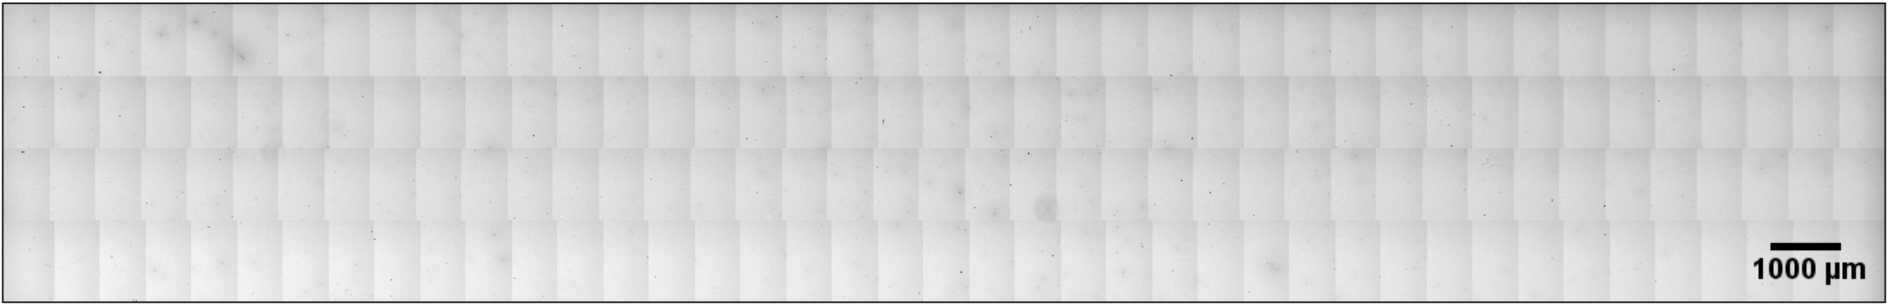
\includegraphics[width=1.0\textwidth]{Figs/cuantificaciondefectos/banda_NIR.png}
	\caption{Imagen de la banda NIR del filtro obtenida mediante un \textit{Tile scan} de 26.37 mm x 4.16 mm, compuesta por 164 \textit{tiles}, con la intensidad de la lámpara configurada en 50\% y el tiempo de exposición de la cámara fue de 150 ms.}
	\label{fig:tilebandanir}
\end{figure}

La adquisición de las imágenes de cada banda considerando el tiempo de seleccionar el área a adquirir, la elección de los parámetros de adquisición, etc. tuvo una duración de aproximadamente 10 minutos por banda. A continuación se explican algunas consideraciones importantes que se tuvieron respecto de los formatos de las imágenes y de los tipos de datos así como su precisión:
\begin{itemize}
\justifying
\item Cada barrido completo de una banda es guardado por el software de Zeiss en un archivo de extensión .czi que contiene toda la \textit{metadata} como la información referida a la configuración del microscopio utilizada. Dicho archivo puede ser manipulado con el software de Zeiss, ó con el \href{https://imagej.net/Fiji}{Fiji-ImageJ} (distribución del software \href{https://imagej.nih.gov/ij/}{ImageJ} con \textit{plugins}) ó a través del lenguaje \textit{python} utilizando la librería \href{https://pypi.org/project/czifile/}{\textit{czifile}} (Ejemplo sencillo: \href{https://github.com/jrr1984/defects_analysis/blob/master/zeiss_cfi.ipynb}{\faGithub}).
\item El archivo .czi de la banda completa además contiene todas las \textit{tiles} del barrido que pueden ser exportadas como archivos individuales utilizando las herramientas de procesamiento del software de Zeiss \cite{tilezeiss}. Es muy importante exportar dichas imágenes eligiendo un formato de imagen que no modifique la calidad de la imagen original, esto es, que no se pierda precisión sobre los valores de intensidad de cada píxel. 
\end{itemize}

%%%%%%%%%%%%%%%%%%%%%%%%%%%%%%%%%%%%%%%%%%%%%%%%%%%%%%%%%%%%%%%%%%%%%%%%%%%%%%%%%%%%%%%%%%%%%%%%%%%%%%%%%%%%%%%%%%%%%%%%%%%%%%%%%%%%%%%%%%%%%%%%%%%%%%%%%%%%%%%%%%%%%%%%%%%%%%%%%%%%%%%%%%%%%%%%%%%%%%%%%%%%%%%%%%%%%%%%%%%%
\singlespacing
\section{Iluminación no uniforme del microscopio}
\label{sec:ilumnou}
\spacing{1.5}

\hspace{0.5cm}La eficiencia en la aplicación de un algoritmo de segmentación\footnote{En el contexto de la presente tesis, el término segmentación hace referencia a la identificación individual de cada defecto presente en una imagen.} de defectos en las imágenes individuales de cada banda adquiridas depende fuertemente de la distribución de los valores de intensidad de una imagen que permiten distinguir a los defectos del fondo de la imagen. A continuación se da una breve explicación sobre las consecuencias de la iluminación no uniforme del microscopio sobre una muestra y como esto repercute en la detección posterior de los defectos. Luego se explica el procesamiento de las imágenes realizado para obtener la cuantificación de los defectos de cada banda del filtro.

Las imágenes de microscopía pueden estar corrompidas por las variaciones de intensidad debido a las imperfecciones inherentes del proceso de formación de imágenes. Estas variaciones de intensidad pueden venir dadas por la iluminación no uniforme de la muestra, por la orientación misma de la muestra al montarla sobre la platina del microscopio ó por el efecto de \textit{vignetting} que se materializa con la aparición de bordes negros en las imágenes y que es propio de la configuración del sensor de la cámara. Estos efectos pueden dar lugar a falsos positivos en el proceso de segmentación de los defectos, lo que constituye un grave problema a solucionar (Ver Sección \ref{sec:tthresh}).

La desalineación de alguno de los componentes que se encuentran en el camino óptico entre la fuente de luz y el sensor de la cámara con el que se adquieren las imágenes (Ver Figura \ref{fig:micczeiss}), es una causa muy importante de la iluminación no uniforme de la muestra que se está analizando. En la Figura \ref{fig:ejnounif} se puede observar un ejemplo de una imagen micróscopica adquirida con una iluminación no uniforme.
	\begin{figure}[H]
		\begin{floatrow}
			\ffigbox{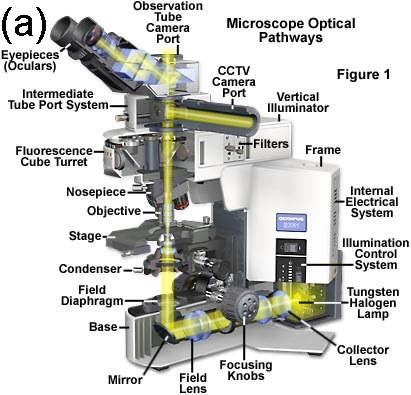
\includegraphics[scale=0.5]{Figs/defectosZEISS/opticalpaths.jpg}}{\caption{Camino óptico de la luz desde su fuente de emisión hasta la detección en el sensor de una cámara digital. Adaptado de \href{https://bit.ly/2xrh8Jh}{https://bit.ly/2xrh8Jh}}\label{fig:micczeiss}}
			\ffigbox{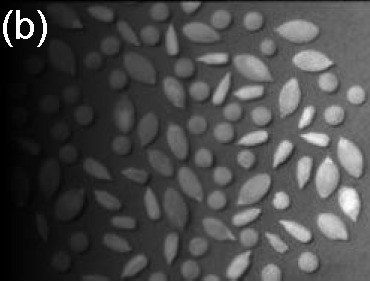
\includegraphics[scale=0.5]{Figs/cuantificaciondefectos/ilumnoun.png}}{\caption{Ejemplo de imagen de microscopía con una iluminación no uniforme.}\label{fig:ejnounif}}
		\end{floatrow}
	\end{figure}
	
Una imagen de microscopía adquirida idealmente con una iluminación uniforme perfecta tendría una imagen de fondo (\textit{background image}) como la que se muestra en la Figura \ref{fig:fondideal}. La imagen de fondo es una imagen que contiene en cada píxel la información de la iluminación del microscopio bajo ciertas condiciones de intensidad de la fuente de luz y del tiempo de integración del sensor de la cámara utilizado. Experimentalmente, dicha imagen puede ser obtenida colocando un portaobjeto sin la muestra, en las mismas condiciones de iluminación y foco (misma distancia muestra-objetivo). Si dicha imagen de fondo experimental no pudiera ser adquirida pero se cuenta con un gran número de imágenes adquiridas bajo las mismas condiciones experimentales, una imagen de fondo puede ser generada tomando la mediana del conjunto de imágenes como se explica en la subsección \ref{sec:genimf}.

Para medir la uniformidad de la iluminación se utilizan los histogramas de las imágenes. Una imagen monocromática es manipulada computacionalmente como una matriz donde cada elemento de la matriz representa el valor de intensidad de dicho píxel asociado. El histograma de una imagen es la representación de la distribución de los valores de intensidad de la misma y se lo define como el número de píxeles presentes en una imagen con un cierto valor de intensidad.

En la Figura \ref{fig:fondideal} se muestra una imagen de fondo ficticia que tendría una iluminación ideal uniforme, sin problemas de  \textit{vignetting} y sin considerar el ruido de Poisson. Dicha imagen tiene un histograma como el que se muestra en la Figura \ref{fig:histbgteo}, en el que se puede observar que todos los píxeles de la imagen tienen el mismo valor de intensidad, lo que demuestra que el fondo es perfectamente homogéneo.
	\begin{figure}[H]
		\begin{floatrow}
			\ffigbox{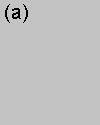
\includegraphics[width=3.0cm,height=3.0cm]{Figs/defectosZEISS/bg_teorico.png}}{\caption{Imagen de fondo con una iluminación uniforme ideal y sin problemas de \textit{vignetting}. }\label{fig:fondideal}}
			\ffigbox{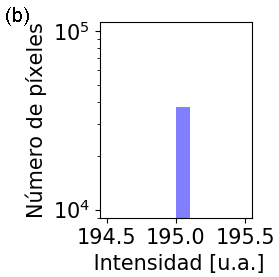
\includegraphics[scale=0.7]{Figs/defectosZEISS/hist_bg_teorico.png}}{\caption{Histograma de la intensidad de los píxeles de la imagen de fondo ideal.}\label{fig:histbgteo}}
		\end{floatrow}
	\end{figure}
En adelante, el fondo de cada imagen será denominado el \textit{background} de la imagen, para diferenciarlo de los defectos que se encuentran en lo que en adelante se llamará el \textit{foreground} de la imagen. Para resaltar la importancia de la corrección de la iluminación no uniforme y del \textit{vignetting}, supongamos una imagen ficticia de alguna banda del filtro analizado en la presente tesis, adquirida con una iluminación de fondo uniforme ideal y sin problemas de \textit{vignetting}, donde se puedan observar dos defectos en color negro (Ver Figura \ref{fig:ideal2def}).
	\begin{figure}[H]
		\begin{floatrow}
			\ffigbox{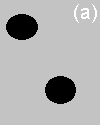
\includegraphics[width=4.0cm,height=4.0cm]{Figs/defectosZEISS/img_ideal_2defectos.png}}{\caption{Imagen con dos defectos con una iluminación uniforme ideal y sin problemas de \textit{vignetting}. }\label{fig:ideal2def}}
			\ffigbox{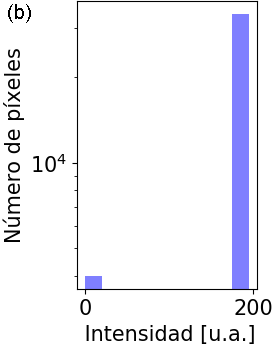
\includegraphics[scale=0.7]{Figs/defectosZEISS/hist_bg_condefectos_teorico.png}}{\caption{Histograma de la intensidad de los píxeles de la imagen con dos defectos con una iluminación uniforme ideal y sin problemas de \textit{vignetting}.}\label{fig:histideal2def}}
		\end{floatrow}
	\end{figure}
En la Figura \ref{fig:histideal2def} se muestra el histograma de la intensidad de los píxeles de la imagen con dos defectos con una iluminación uniforme ideal y sin problemas de \textit{vignetting}. En dicho histograma se distingue de forma binaria el \textit{foreground} (defectos) con valores de intensidad iguales a 0, del \textit{background} con valores de intensidad iguales a 195. Bajo estas condiciones ideales, la segmentación de los defectos puede ser realizada de inmediato eligiendo cualquier umbral de intensidad que se encuentre entre el \textit{foreground} y el \textit{background}. 

A continuación se explica la corrección de la iluminación no uniforme del microscopio en las imágenes individuales de cada banda adquiridas.

%%%%%%%%%%%%%%%%%%%%%%%%%%%%%%%%%%%%%%%%%%%%%%%%%%%%%%%%%%%%%%%%%%%%%%%%%%%%%%%%%%%%%%%%%%%%%%%%%%%%%%%%%%%%%%%%%%%%%%%%%%%%%%%%%%%%%%%%%%%%%%%%%%%%%%%%%%%%%%%%%%%%%%%%%%%%%%%%%%%%%%%%%%%%%%%%%%%%%%%%%%%%%%%%%%%%%%%%%%%%
\singlespacing
\section{Pre-pocesamiento de las imágenes de cada banda espectral }
\label{sec:preproc}
\spacing{1.5}

\hspace{0.5cm}El análisis de las imágenes fue realizado sobre cada \textit{tile} individual del barrido completo de una banda, dado que su tamaño típico es de 3 MB por lo que el procesamiento en la computadora es mucho más rápido que el de analizar las imágenes de una banda completa\footnote{Vale aclarar que las imágenes completas ya sea de una banda ó las del filtro completo, fueron el resultado de realizar un \textit{stitching} de todas las \textit{tiles} individuales de cada adquisición y, fueron procesadas de esta manera simplemente para optimizar su \textit{visualización} pero no para realizar el análisis ni detección de defectos sobre las mismas.}, de tamaños típicos de 1 GB ó del filtro completo que tienen más de 5 GB.

El pre-procesamiento de las imágenes individuales de cada banda espectral consistió en la corrección de la iluminación no uniforme del microscopio. Dicha corrección fue realizada a partir de la normalización de  las imágenes individuales del barrido con una imagen de fondo \cite{Nordenfelt}. Este pre-procesamiento consistió de las siguientes dos etapas que se explican a continuación:
\begin{enumerate}
\justifying
\item Generación de la imagen de fondo.
\item Normalización de las imágenes individuales del barrido de una banda con la imagen de fondo.
\end{enumerate}

%%%%%%%%%%%%%%%%%%%%%%%%%%%%%%%%%%%%%%%%%%%%%%%%%%%%%%%%%%%%%%%%%%%%%%%%%%%%%%%%%%%%%%%%%%%%%%%%%%%%%%%%%%%%%%%%%%%%%%%%%%%%%%%%%%%%%%%%%%%%%%%%%%%%%%%%%%%%%%%%%%%%%%%%%%%%%%%%%%%%%%%%%%%%%%%%%%%%%%%%%%%%%%%%%%%%%%%%%%%%%%%%%%%%%%%%%%%%%%%%%%%%%%%%%%%%%%%%%%%%%%%%%%%%%%%%%%%
\singlespacing
\subsection{Generación de la imagen de fondo: \href{https://github.com/jrr1984/defects_analysis/blob/master/bg.py}{\faGithub}}
\label{sec:genimf}
\spacing{1.5}

\hspace{0.5cm}Se construyó computacionalmente la imagen de fondo de cada banda a partir de tomar la mediana para cada píxel de todas las imágenes individuales adquiridas de la banda. Esta imagen de fondo contiene la información de la no uniformidad de la iluminación del microscopio. Dicha imagen debe ser generada para cada banda en particular ya que cada una de las bandas fue adquirida en ciertas condiciones de intensidad de la fuente de luz y del tiempo de integración de la cámara. 

En la Figura \ref{fig:bgazul} se muestra la imagen de fondo generada para la banda azul, cuya intensidad de la fuente de luz fue configurada en 30$\%$ y el tiempo de integración de la cámara fue de 40 ms. Los dos discos concéntricos que podrían ser anillos de difracción, recuadrados en color azul en la imagen, son resultado de algún defecto del microscopio, ya advertido por otros usuarios del equipo. Dichos discos fueron observados en la adquisición de las cinco bandas. 
	\begin{figure}[H]
		\begin{floatrow}
			\ffigbox{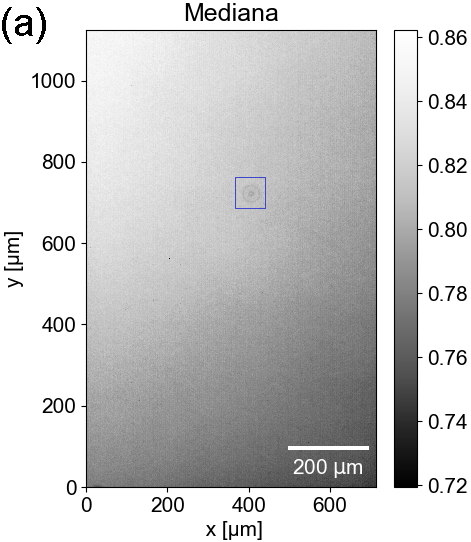
\includegraphics[scale=0.9]{Figs/defectosZEISS/bg_azul.png}}{\caption{Imagen de fondo de la banda azul del filtro obtenida tomando la mediana para cada píxel de todas las imágenes del barrido.}\label{fig:bgazul}}
			\ffigbox{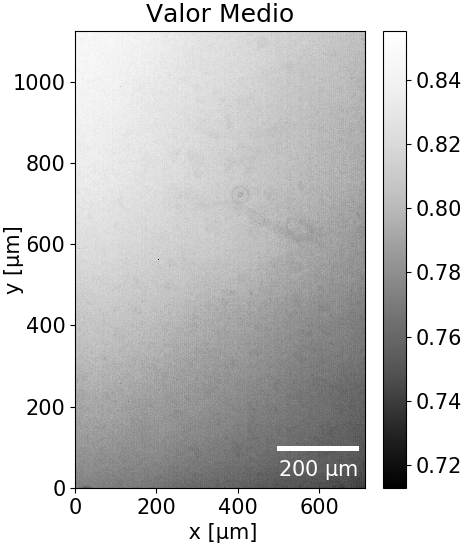
\includegraphics[scale=0.9]{Figs/defectosZEISS/bg_azul_mean.png}}{\caption{Imagen de fondo de la banda azul del filtro obtenida tomando el valor medio para cada píxel de todas las imágenes del barrido. Se redondearon en color verde las manchas que representan los \textit{outliers} de la imagen.}\label{fig:bgazulmean}}
		\end{floatrow}
	\end{figure}
Al mismo tiempo, se observa en la imagen de fondo de la Figura \ref{fig:bgazul} que la iluminación del microscopio no es idealmente uniforme sino que presenta un rango de valores de intensidad que contienen píxeles más brillantes (extremo superior izquierdo) en conjunto con píxeles más oscuros (extremo inferior derecho). Esto último puede ser el efecto de alguna desalineación de la configuración del microscopio.

En la Figura \ref{fig:comparhists} se muestran los histogramas de la intensidad de los píxeles de las imágenes de fondo generadas a partir de tomar la mediana y el valor medio. En la misma figura se graficaron las curvas de densidad de la intensidad estimadas a partir de los datos originales. Se observa que la imagen de fondo generada con el valor medio tiene una mayor cantidad de píxeles más oscuros que la imagen de fondo generada con la mediana. Los valores atípicos (en inglés \textit{outliers}) de intensidad influencian enormemente el valor medio de los datos. Dichos \textit{outliers} pueden observarse como manchas presentes (algunas redondeadas en color verde) en la imagen de fondo generada a partir del valor medio de la Figura \ref{fig:bgazulmean}. En la curva de densidad esto se refleja en el hecho de que la curva del valor medio tiene una mayor concentración en valores de intensidades más chicos que la curva de la mediana. Ahora bien, la curva de densidad de la imagen de la mediana muestra que la generación de la imagen de fondo tomando la mediana es una forma exitosa de evitar incluir los \textit{outliers} en la imagen. Resulta fundamental deshacerse de estos \textit{outliers} en la imagen de fondo para no corromper las imágenes individuales originales del barrido. Esto es, si se utilizara la imagen de fondo del valor medio para corregir la iluminación no uniforme en las imágenes individuales, las mismas tendrían luego los \textit{outliers} presentes lo cual sería catástrofico para la aplicación del algoritmo de segmentación de los defectos.
\begin{figure}[H]
	\centering
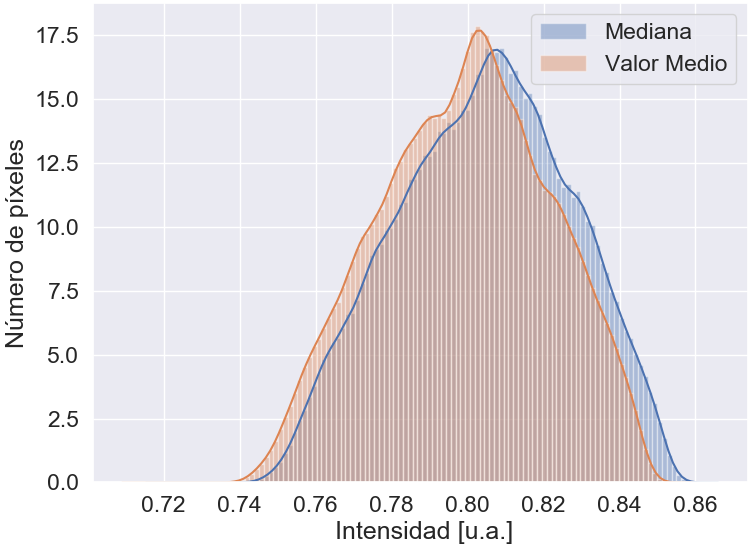
\includegraphics[scale=0.55]{Figs/defectosZEISS/comparhistsmedi.png}
\caption{Histogramas de las imágenes de fondo de la banda azul del filtro generadas a partir de tomar el valor medio y la mediana para cada píxel del conjunto de imágenes de la banda. El eje vertical se encuentra normalizado por el máximo valor de la frecuencia de píxeles para un cierto valor de intensidad.}
\label{fig:comparhists}
\end{figure}	
	
\singlespacing
\subsection{Normalización de las imágenes individuales del barrido de una banda con la imagen de fondo \href{https://github.com/jrr1984/defects_analysis/blob/master/bg_normalization.py}{\faGithub}}
\label{subs:nm}
\spacing{1.5}

\hspace{0.5cm} Con la imagen de fondo de cada banda ya generada, se normalizaron las imágenes originales del barrido completo de cada banda\cite{Nordenfelt} con el objetivo de corregir la iluminación no uniforme del microscopio y para eliminar la reflexión no deseada del objetivo del microscopio presente en todas las imágenes (discos concéntricos de la imagen \texttt{b)} de la Figura \ref{fig:bgazul}).
\begin{figure}[H]
	\centering
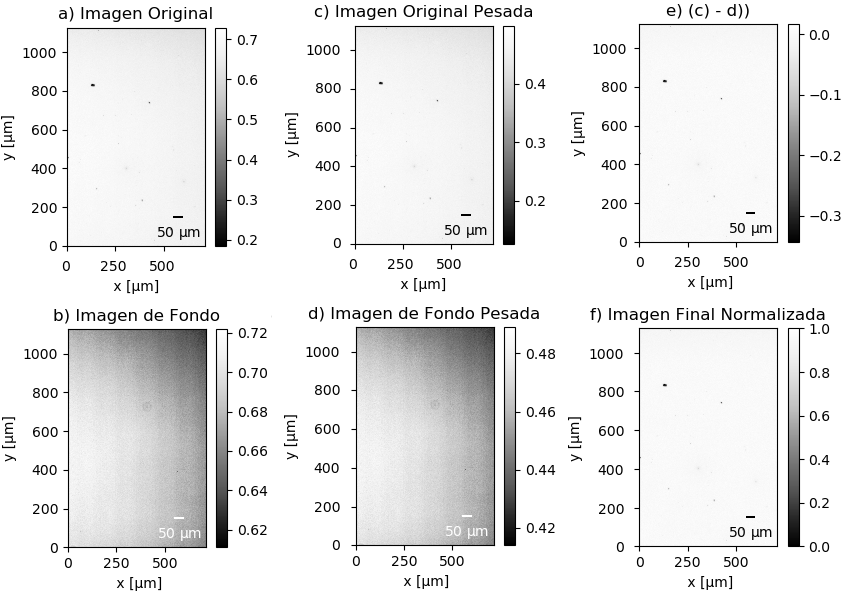
\includegraphics[scale=0.98]{Figs/defectosZEISS/correccionilum/NIR/1.png}
\caption{Imágenes del proceso de corrección de la iluminación no uniforme. \texttt{a)} Imagen original individual de la banda NIR. \texttt{b)} Imagen de fondo de la banda NIR. \texttt{c)} Imagen original multiplicada por el valor medio de la imagen de fondo. \texttt{d)} Imagen de fondo multiplicada por el valor medio de la imagen original. \texttt{e)} Imagen resultante de la diferencia entre las imágenes \texttt{c)} y \texttt{d)}. \texttt{e)} Imagen final normalizada resultado de la expansión del histograma de intensidades.}
\label{fig:correcilumims}
\end{figure}	
 En la Figura \ref{fig:correcilumims} se muestran las operaciones del proceso de normalización de una imagen individual (\textit{tile}) del barrido completo de la banda NIR. El mismo proceso fue realizado para cada imagen individual de cada banda adquirida con su respectiva imagen de fondo, de acuerdo a las siguientes operaciones:
\begin{itemize}
\justifying
\item Se calculó el valor medio de la intensidad de la imagen de fondo (\textit{bg\_img}, ver imagen \texttt{b)}) y de la imagen individual (\textit{tile\_img}, ver imagen \texttt{a)}) de una banda a normalizar. Esto es, se calculó la media aritmética de todos los elementos de matriz que representan a cada imagen, que es el resultado de la división entre la suma de todos los elementos de la matriz y el número total de los mismos.
\item Se multiplicó la imagen de fondo por el valor medio de la imagen individual y viceversa, es decir:
\begin{equation}
\textit{bg\_pes} = mean(\textit{tile\_img})\hspace{2pt} . \hspace{2pt}\textit{bg\_img}
\end{equation}
\begin{equation}
\textit{tile\_pes} = mean(\textit{bg\_img})\hspace{2pt} . \hspace{2pt}\textit{tile\_img},
\end{equation}
donde \textit{bg\_pes} (Ver imagen \texttt{d)}) y \textit{tile\_pes} (Ver imagen \texttt{c)}) son la imagen de fondo y la imagen individual pesadas con la contribución del valor medio de la imagen correspondiente.
\item Se corrigió la iluminación no uniforme de la imagen original (Ver imagen \texttt{e)}), cuya imagen resultante se la denomina \textit{dif}:
\begin{equation}
\textit{dif} = \textit{tile\_pes} - \textit{bg\_pes}
\end{equation}
\item Finalmente, para maximizar el contraste de la imagen, es decir para aumentar el rango dinámico de la imagen, se realizó la expansión del histograma (\cite{anilfund}) que consiste en una transformación lineal para expandir el intervalo comprendido entre los valores mínimo y máximo de intensidad presentes en la imagen, a todo el rango posible entre 0 y 1 (Ver Ecuación \ref{eq:histexpp}). Para ello, se definió el mínimo valor de la intensidad en 0 (en un rango de valores de intensidad entre 0 y 1):
\begin{equation}
	\textit{min\_dif} = \textit{dif} - min(\textit{dif}),
\end{equation}
donde min(\textit{dif}) es el mínimo valor de intensidad de la imagen \textit{dif}. A la imagen resultante \textit{min\_dif} se la normaliza de la siguiente manera:
\begin{equation}
	\textit{imagen\_final} = \frac{\textit{min\_dif}}{max(\textit{dif})-min(\textit{dif})} = \frac{\textit{dif} - min(\textit{dif})}{max(\textit{dif})-min(\textit{dif})},
	\label{eq:histexpp}
\end{equation}
donde max(\textit{dif}) es el máximo valor de intensidad de la imagen \textit{dif} e \textit{imagen\_final} es la imagen resultante del proceso de normalización.
\end{itemize}

Se hace notar que el proceso de corrección de la iluminación no uniforme y del \textit{vignetting} resultó fundamental para poder aplicar el algoritmo de detección de los defectos, esto es para distinguir el \textit{foreground} del \textit{background}, como se explicó en la sección \ref{sec:ilumnou}. Para ejemplificar esto y para ilustrar la operación de la expansión del histograma de la ecuación \ref{eq:histexpp}, en la Figura \ref{fig:defecthi} se muestra una región con un defecto de la imagen original y de la final así como los histogramas de intensidad de los píxeles de la diagonal de la misma región asociados.


\begin{figure}[H]
	\centering
	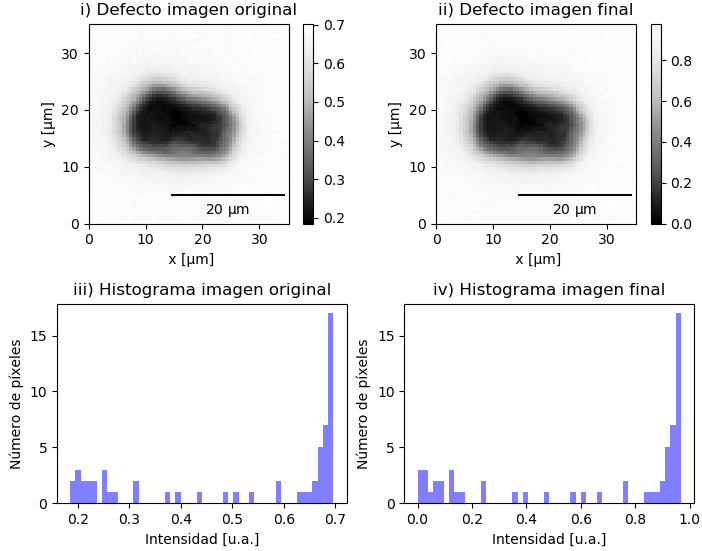
\includegraphics[scale=1.0]{Figs/defectosZEISS/correccionilum/defectoehist.png}
	\caption{\texttt{i)} Imagen original de una región con un defecto. \texttt{ii)} Imagen resultante del proceso de normalización de la misma región que \texttt{i)}. \texttt{iii)} Histograma de los píxeles de la diagonal de la imagen \texttt{i)}. \texttt{iv)} Histograma de los píxeles de la diagonal de la imagen \texttt{ii)}.}
	\label{fig:defecthi}
\end{figure}

De la comparación entre los histogramas \texttt{iii)} y \texttt{iv)} se observa que el rango de intensidades de los píxeles de la región con un defecto de la imagen original se extiende desde el intervalo [0.19,0.70] al intervalo [0.00,0.98] en la imagen final\footnote{Para la imagen completa, el rango se extiende desde [0.19,0.73] para la imagen original al rango [0.00,1.00] de la imagen final, es decir el rango de intensidades de la imagen original se extiende a todo el rango posible de acuerdo a la ecuación \ref{eq:histexpp} de la expansión del histograma.}. De esta manera, se mejora el contraste de la imagen y la distinción entre el \textit{foreground} (defectos) y el \textit{background} se puede realizar ajustando un umbral de intensidad  (\textit{threshold}). A continuación se explica el criterio de elección del método del \textit{threshold} aplicado y luego se describe el algoritmo de detección de los defectos y su cuantificación.
%%%%%%%%%%%%%%%%%%%%%%%%%%%%%%%%%%%%%%%%%%%%%%%%%%%%%%%%%%%%%%%%%%%%%%%%%%%%%%%%%%%%%%%%%%%%%%%%%%%%%%%%%%%%%%%%%%%%%%%%%%%%%%%%%%%%%%%%%%%%%%%%%%%%%%%%%%%%%%%%%%%%%%%%%%%%%%%%%%%%%%%%%%%%%%%%%%%%%%%%%%%%%%%%%%%%%%%%%%%%
\singlespacing
\section{Criterio de elección del \textit{threshold} \href{https://github.com/jrr1984/defects_analysis/blob/master/try_all_thresholds.py}{\faGithub}}
\label{sec:tthresh}
\spacing{1.5}

\hspace{0.5cm}Con las imágenes pre-procesadas la detección de los defectos fue realizada utilizando algoritmos de procesamientos de imágenes. En particular se utilizaron algoritmos de \textit{thresholding} que determinan un umbral de intensidad a partir del cual se crea una imagen binaria que distingue el \textit{background} de los defectos \cite{shapi}.

Para determinar el umbral de intensidad óptimo para todas y cada una de las imágenes individuales de una banda se utilizó el método \textit{try\_all\_threshold} de la librería \textit{scikit-image} del lenguaje \textit{python} \cite{van2014scikit}. Dicho método permite realizar pruebas inmediatas de los umbrales más utilizados en la literatura como se explica a continuación. Se hace notar que si bien se podrían haber utilizado distintos \textit{thresholds} para cada imagen ó para distintos conjuntos de imágenes de una misma banda, se decidió elegir un sólo método de umbral para todas y cada una de las bandas para poder automatizar la aplicación del algoritmo de detección de los defectos y de la posterior asociación de incertezas a los resultados.

El criterio de elección del método del umbral fue adoptado a partir de la inspección visual. Se observó visualmente el resultado (en adelante \textit{output}) de la aplicación de los distintos \textit{thresholds} para cada imagen de cada banda. A continuación se muestran algunas imágenes representativas en conjunto con el \textit{output} de la aplicación de los distintos \textit{thresholds} para explicar el criterio de elección del umbral aplicado a todas las imágenes de todas las bandas:
\begin{enumerate}
\justifying
\item Se descartaron los \textit{thresholds} a partir de los cuales algunas de las imágenes binarias generadas contenían una gran cantidad de falsos positivos. Esto último resultó ser el caso de los métodos \textit{Li}\cite{Lie}, \textit{Mean}\cite{Glasmean} y \textit{Otsu}\cite{otsuu}, como se puede observar en la Figura \ref{fig:threshcom}. Por el motivo contrario, es decir por no contener ningún defecto en algunas de las imágenes binarias generadas, el umbral \textit{Minimum}\cite{pericles} fue descartado.
\begin{figure}[H]
	\centering
	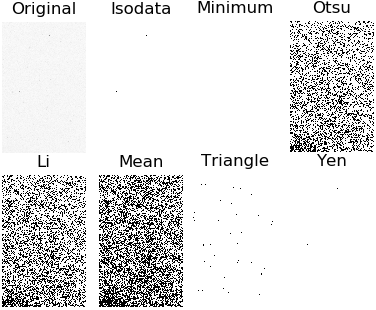
\includegraphics[scale=1.5]{Figs/defectosZEISS/thresh_comparison.png}
	\caption{Figura del \textit{output} del método \textit{try\_all\_threshold} de la librería \textit{scikit-image} del lenguaje \textit{python} (Ver \href{https://github.com/jrr1984/defects_analysis/blob/master/try_all_thresholds.py}{\faGithub}).} 
	\label{fig:threshcom}
\end{figure}

\item Si bien en la gran mayoría de las imágenes los métodos \textit{Isodata}\cite{ridler} y \textit{Triangle}\cite{triang} no detectaban falsos positivos, el único \textit{threshold} que no detectó ningún falso positivo para todas las imágenes de todas las bandas fue el del método \textit{Yen}. Esto permitió automatizar el cálculo del umbral para todas las imágenes. Por ejemplo en la Figura \ref{fig:threshcom2} se muestra una región de una imagen con 2 defectos detectados por inspección visual y el método \textit{Yen} fue el único capaz de detectarlos de forma singular.

\begin{figure}[H]
	\centering
	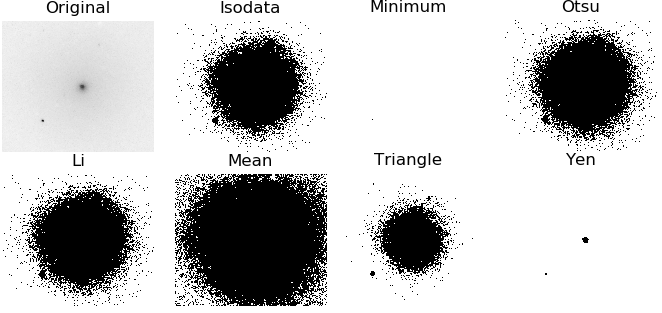
\includegraphics[scale=0.8]{Figs/defectosZEISS/thresh_vivos_compar3.png}
	\caption{Región de una imagen individual en conjunto con el \textit{output} del método \textit{try\_all\_threshold} de la librería \textit{scikit-image} del lenguaje \textit{python} (Ver \href{https://github.com/jrr1984/defects_analysis/blob/master/try_all_thresholds.py}{\faGithub}).} 
	\label{fig:threshcom2}
\end{figure}
%# de defectos por metodo: yen,isodata,triangle
%2828,4439,274176  ROJO
%4015,6674,156695 PANC
%5727,11010,234359 VERDE
%19918,40505, AZUL
\end{enumerate}


\hspace{0.5cm}Una vez determinado el \textit{threshold} aplicable a todas las imágenes de todas las bandas, se desarrolló el algoritmo de detección y cuantificación de los defectos del filtro.

%%%%%%%%%%%%%%%%%%%%%%%%%%%%%%%%%%%%%%%%%%%%%%%%%%%%%%%%%%%%%%%%%%%%%%%%%%%%%%%%%%%%%%%%%%%%%%%%%%%%%%%%%%%%%%%%%%%%%%%%%%%%%%%%%%%%%%%%%%%%%%%%%%%%%%%%%%%%%%%%%%%%%%%%%%%%%%%%%%%%%%%%%%%%%%%%%%%%%%%%%%%%%%%%%%%%%%%%%%%%%%%%%%%%%%%%%%%%%%%%%%%%%%%%%%%%%%%%%%%%%%%%%%%%%%%%%%%
\singlespacing
\section{Algoritmo de detección y cuantificación de los defectos \href{https://github.com/jrr1984/defects_analysis/blob/master/defects_thresholding.py}{\faGithub}}
\label{sec:secalg}
\spacing{1.5}

\hspace{0.5cm}En esta sección se explica el algoritmo utilizado para la detección y cuantificación de los defectos del filtro. El diagrama de flujo del algoritmo aplicado se muestra en la Figura \ref{fig:diagflujoalgor}. 

\begin{figure}[H]
\centering
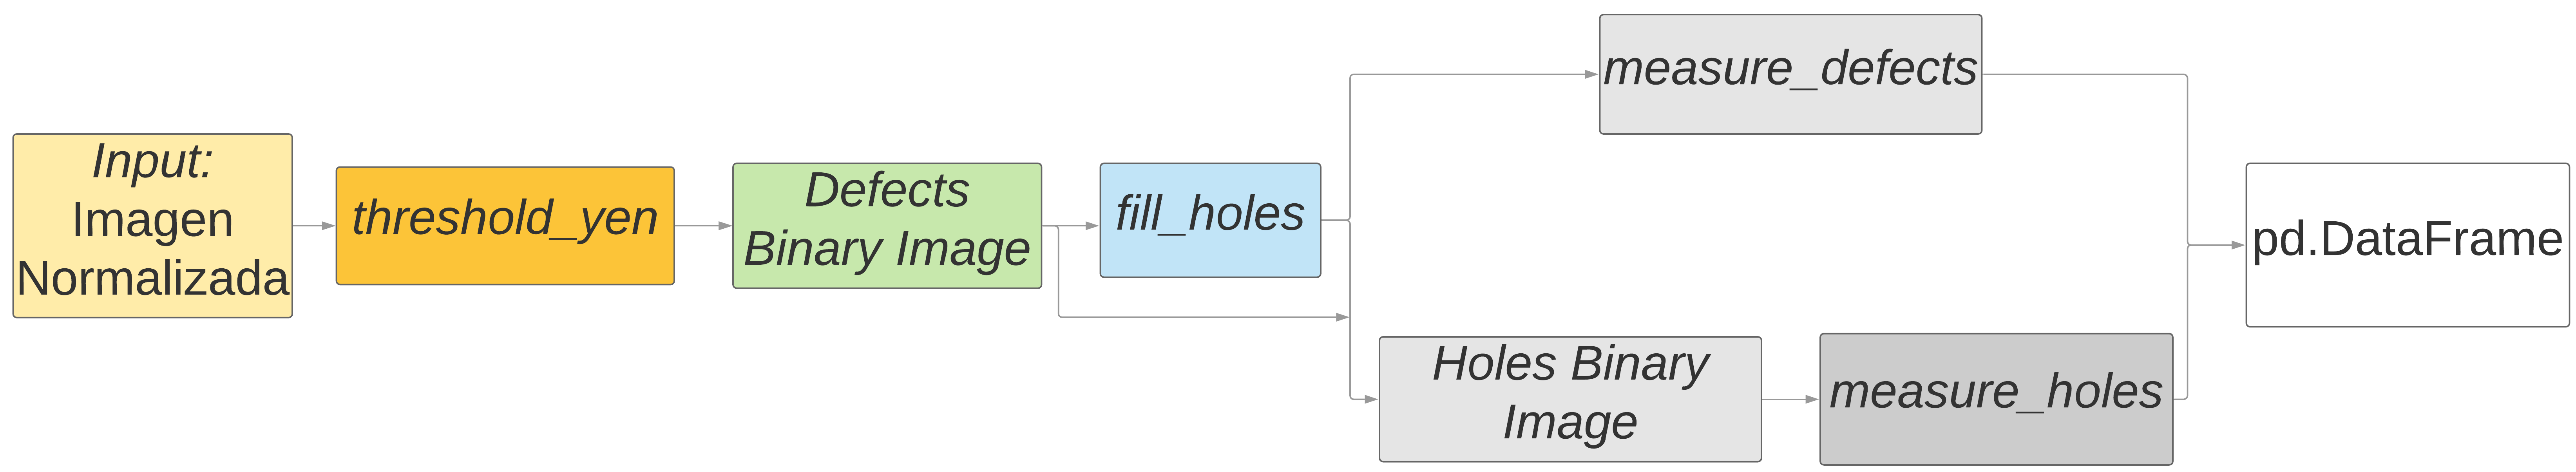
\includegraphics[scale=0.75]{Figs/cuantificaciondefectos/diag_flujoalgor.png}
\caption{Diagrama de flujo del algoritmo de detección y cuantificación de los defectos del filtro.}
\label{fig:diagflujoalgor}
\end{figure}


\begin{figure}[H]
\centering
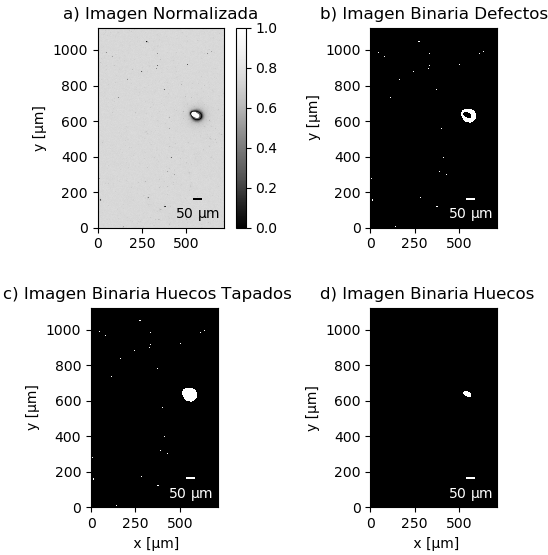
\includegraphics[scale=1.1]{Figs/defectosZEISS/algor_defecs.png}
\caption{\texttt{a)} Imagen normalizada de la banda celeste que contiene un agujero.  \texttt{b)} Imagen binaria generada a partir del \textit{threshold} de \textit{Yen}. \texttt{c)} Imagen con los agujeros de la imagen \texttt{b)} tapados con el método \textit{binary\_fill\_holes} de la clase \textit{ndimage} de la librería \textit{scipy} del lenguaje \textit{python}. \texttt{d)} Imagen binaria con el agujero detectado.}
\label{fig:flujoalgo}
\end{figure} 

Utilizando el diagrama de flujo de la Figura \ref{fig:diagflujoalgor} y la Figura \ref{fig:flujoalgo} como guías didácticas, a continuación se explican los pasos del algoritmo aplicado para cada imagen individual de cada banda:
\begin{enumerate}
\justifying
\item \texttt{INPUT: Imagen Normalizada.} Se lee la imagen normalizada. En la imagen \texttt{a)} de la Figura \ref{fig:flujoalgo} se muestra una imagen normalizada de la banda azul que contiene el agujero más grande encontrado en el filtro (caracterizado espectralmente en el Capítulo \ref{chap:microsp}) y otros defectos de transmisión (manchas negras) más pequeños. En consecuencia, la imagen es representativa de lo que sería el caso más general de la aplicación del algoritmo para detectar tanto defectos de transmisión como agujeros. 
\item \texttt{\textit{threshold\_yen}.} Se calcula el \textit{threshold} de \textit{Yen} con el método \textit{threshold\_yen} de la librería \textit{scikit-image}. En la Figura \ref{fig:histalgor} se muestra el histograma de intensidad de píxeles de la imagen, con el eje vertical en escala logarítmica. La línea vertical roja indica el valor calculado del \textit{threshold} de \textit{Yen} que para esta imagen de ejemplo su valor fue de 0.57. Se hace notar que dicho valor de intensidad umbral es global de toda la imagen y para cada imagen se calcula un \textit{threshold} de \textit{Yen} individual.

\begin{figure}[H]
\centering
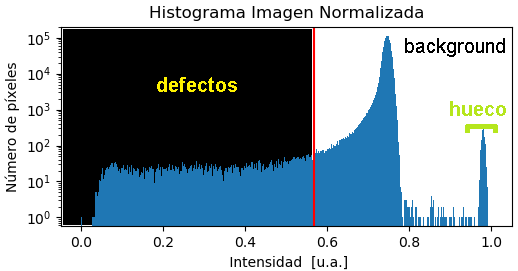
\includegraphics[scale=1.65]{Figs/defectosZEISS/hist_algor_agujero.png}
\caption{Histograma de intensidad de los píxeles de la imagen \texttt{a)} de la Figura \ref{fig:flujoalgo}, con el eje vertical en escala logarítmica. La línea roja vertical indica el valor del \textit{threshold} de \textit{Yen} para dicha imagen.}
\label{fig:histalgor}
\end{figure}

\item \texttt{Defects Binary Image.}Se genera una imagen binaria de la imagen normalizada como se muestra en la imagen \texttt{c)} de la Figura \ref{fig:flujoalgo}. Para cada píxel de la imagen normalizada se compara su valor de intensidad con el valor del \textit{threshold} y se asigna un 1 (blanco, \textit{background} y agujeros) si el valor de intensidad del píxel es mayor que el \textit{threshold} y un 0 (negro, defectos) si ocurre lo contrario. Esto último se puede ver en el histograma de la Figura \ref{fig:histalgor}.
\item \texttt{\textit{fill\_holes}.} Se tapan los agujeros como se muestra en la imagen \texttt{d)} de la Figura \ref{fig:flujoalgo} con el método \textit{binary\_fill\_holes} de la clase \textit{ndimage} de la librería \textit{scipy} del lenguaje \textit{python} \cite{scipy}.

\hspace{0.5cm}Se hace notar que en el contexto de imágenes binarias un defecto de transmisión es un objeto matricial de ciertas dimensiones en píxeles cuyos elementos de matriz son todos iguales a 1 (color blanco). Y, un agujero es un objeto matricial cuyo borde tiene elementos de matriz iguales a 1 (color blanco) pero los elementos de matriz del interior de dicho borde son iguales a 0 (color negro). Lo que el método \textit{binary\_fill\_holes} realiza es encontrar objetos que cumplan la condición matricial de un agujero y llenar su interior de píxeles blancos. El tamaño del agujero a tapar puede ser elegido por el usuario a partir de las dimensiones de la matriz de píxeles blancos utilizada. Esta matriz es especificada en el argumento \textit{structure} del método \textit{binary\_fill\_holes} y es un parámetro fundamental que debe ser especificado de acuerdo a los requerimientos de calidad óptica del usuario ya que su tamaño define el tamaño mínimo del agujero a detectar. En la presente tesis dicho parámetro fue dejado sin especificar, el método tomó el valor por \textit{default} por lo que todos los agujeros encontrados fueron tapados.

\hspace{0.5cm}A continuación se explica la bifurcación en el algoritmo de la detección de defectos en general por un lado sin discriminar su tipo y la detección específica de agujeros por el otro lado.

\item \texttt{\textit{measure\_defects}}. La detección de los defectos en general fue realizada sobre las imágenes binarias con los agujeros tapados (Ver imagen \texttt{c)} de la Figura \ref{fig:flujoalgo}). En consecuencia, no se distinguieron los agujeros de los defectos de transmisión, sino que todos los defectos fueron considerados defectos de superficie de acuerdo a las especificaciones técnicas de la ISO 10110 (Ver Sección \ref{sec:iso10110}). Por este motivo resultó importante realizar el tapado de los agujeros ya que sino se modificaría el valor del área total de los defectos con estas características, considerando a estos como un solo objeto compuesto por una mancha negra que bordea a un agujero blanco, como por ejemplo de acuerdo al defecto más grande de la Figura \ref{fig:flujoalgo}. Este mismo defecto sin tapar tenía un área (dada por el número de píxeles) de (1065 $\pm$ 6)$\mu m^{2}$ y un diámetro de $(81 \pm 6)\mu m$ pero el mismo agujero tapado, es decir el defecto a estimar, tenía un área de (5174 $\pm$ 160)$\mu m^{2}$ y un diámetro de $(81 \pm 6)\mu m$, por lo que se hubiese obtenido un \% de error.

\hspace{0.5cm}En la imagen binaria con los agujeros tapados, los defectos ya se encontraban segmentados, es decir que los defectos eran regiones aisladas de píxeles blancos conectados entre sí. El método \href{https://scikit-image.org/docs/dev/api/skimage.measure.html#skimage.measure.label}{\textit{measure.label}} etiqueta a cada uno de los defectos cuyas propiedades son calculadas con el método \href{https://scikit-image.org/docs/dev/api/skimage.measure.html#skimage.measure.regionprops_table}{\textit{measure.regionprops\_table}} y luego guardadas en un \href{https://pandas.pydata.org/pandas-docs/stable/reference/api/pandas.DataFrame.html}{\textit{DataFrame}} de la librería \textit{pandas}\cite{pandas}\footnote{Un \textit{DataFrame} de \textit{pandas} es una estructura de datos que permite una rápida visualización de los datos como en una planilla de excel y que tiene una gran familia de métodos a su disposición para realizar un análisis cuantitativa de los datos.}. Las propiedades de los defectos calculadas fueron el área y el diámetro equivalente\footnote{Muchas otras propiedades podrían haber sido también calculadas automáticamente pero no fueron necesarias en el presente trabajo (Ver \href{https://github.com/scikit-image/scikit-image/blob/master/skimage/measure/\_regionprops.py\#L643}{\textit{measure.regionprops}}).}:
\begin{itemize}
\justifying
\item El área fue calculada a partir del número de píxeles totales que conforman al defecto, siendo un píxel la menor unidad homogénea en color que forma parte de una imagen digital. Así por ejemplo el defecto más grande de la imagen \texttt{c)} de la Figura \ref{fig:flujoalgo} estaba formado por 15068 píxeles. De acuerdo a la calibración del microscopio el área de 1 píxel equivale a 0.586 $\mu m$ x 0.586 $\mu m$, con lo cual 15068 píxeles = 15068 . $(0.586 \mu m)^{2} \sim 5174 \mu m^{2}$, con una incerteza asociada de 160 $\mu m^{2}$ (Ver Sección \ref{sec:incert}).
\item El diámetro equivalente consiste en el diámetro de un círculo con la misma área calculada en el paso anterior. Igualando dicha área con el área de un círculo, $\pi . (\frac{diametro}{2})^{2}$, se obtiene el diámetro equivalente. Por ejemplo el defecto de la Figura \ref{fig:flujoalgo} tuvo un diámetro de $(81 \pm 6) \mu m$.
\end{itemize} 

\item \texttt{Holes Binary Image}. La imagen binaria de los agujeros segmentados (Ver Imagen \texttt{d)} de la Figura \ref{fig:flujoalgo}) fue generada a partir de tomar la diferencia entre la imagen binaria de los agujeros tapados y la imagen binaria de los defectos. Dicha forma de segmentar los agujeros como objetos matriciales cuyo borde son unos y el interior son ceros resultó ser la forma más eficiente para no obtener una gran cantidad de falsos positivos (detección de agujeros que en realidad no lo son). Con este método el máximo número de agujeros encontrado en una banda fue de 12 con lo cual la verificación de los falsos positivos del método se realiza rápidamente observando visualmente las imágenes en las que fueron detectados. 

\hspace{0.5cm}Párrafo aparte merece la explicación de un método alternativo que se ensayó para intentar segmentar los agujeros pero que arrojaba una gran cantidad de falsos positivos (Ver \href{https://github.com/jrr1984/defects_analysis/blob/master/find_contours_holes_trial.py}{\faGithub}). En el histograma de la Figura \ref{fig:histalgor} se observa claramente la región de valores de intensidad cercanos a la saturación (en escala monocromática de la imagen normalizada) que pertenecen al agujero de la imagen \texttt{a)} de la Figura \ref{fig:flujoalgo}. Aplicando un \textit{threshold} de intensidad de 0.97 se detecta singularmente el agujero de dicha imagen. Ahora bien, este mismo umbral (ó cualquier variación del mismo) aplicado al conjunto de imágenes de la misma banda arroja miles de falsos positivos de tamaños tan grandes como los propios agujeros reales detectados visualmente. Esto ocure pues el fondo de la imagen normalizada contiene regiones conectadas de píxeles con mayor ó igual valor de intensidad que tiene el centro de un agujero. Además, otro motivo por el que se descartó este método es debido a la definición matricial del agujero data anteriormente que supone que cada agujero presente en las imágenes normalizadas tiene un centro blanco con valores de intensidad cercanos a 1 pero que tiene un borde perimetral oscuro.

\hspace{0.5cm}Ahora bien, por un lado se detectaron los agujeros para poder determinar su diámetro y área de forma más precisa que al ser tratados como defectos en general como se explicó en el proceso 5, \texttt{\textit{measure\_defects}}. Además, por otro lado la segmentación de los agujeros permitió ubicarlos espacialmente en el filtro de forma tal de poder caracterizarlos espectralmente como se explica en el Capítulo \ref{chap:microsp}. Esto es, para cada agujero detectado se conocen su ubicación en la imagen que fue hallado y como al mismo tiempo se conoce la posición de cada imagen individual en el barrido completo de una banda, se determinan las coordenadas espaciales del agujero en el filtro. Este \textit{feature} del algoritmo permite rápidamente descartar un filtro si no cumple con las especificaciones técnicas requeridas por la aplicación del usuario final y resulta independiente del inspector de turno del filtro como en el caso de la aplicación de la métrica de \textit{scratc \& dig} (Ver Sección \ref{sec:scanddig}).

\item \texttt{\textit{measure\_holes}} A partir de la imagen segmentada de los agujeros se repite el proceso implementado en el paso del algoritmo \texttt{\textit{measure\_defects}}: se etiquetan a los agujeros y se mide su área y su diámetro equivalente. Dichos resultados son concatenados al \textit{DataFrame} de pandas.
\item \texttt{\textit{pd.DataFrame}.} Los resultados con las incertezas asociadas(Ver Sección \ref{sec:incert}) de los defectos en general y de los agujeros contenidos en un \textit{DataFrame} son exportados en un archivo \textit{pickle}\footnote{Con el módulo \textit{pickle} de python se puede serializar cualquier tipo de objeo de python y guardarse en un archivo \textit{pickle}, de extensión .pkl, que resulta muy eficiente tanto en su escritura como en su lectura.} que fue manipulado utilizando el entorno interactivo de \href{https://ipython.org/notebook.html}{\textit{IPython Notebook}}. Por último, con el método \textit{morphology.remove\_small\_objects} se puede elegir el tamaño de los defectos a incluir en el análisis definitivo dependiendo de la aplicación del usuario final y de la especificación técnica a ser verificada.
\end{enumerate}


%%%%%%%%%%%%%%%%%%%%%%%%%%%%%%%%%%%%%%%%%%%%%%%%%%%%%%%%%%%%%%%%%%%%%%%%%%%%%%%%%%%%%%%%%%%%%%%%%%%%%%%%%%%%%%%%%%%%%%%%%%%%%%%%%%%%%%%%%%%%%%%%%%%%%%%%%%%%%%%%%%%%%%%%%%%%%%%%%%%%%%%%%%%%%%%%%%%%%%%%%%%%%%%%%%%%%%%%%%%%%%%
\singlespacing
\section{Resultados del algoritmo de detección de los defectos de superficie \href{https://github.com/jrr1984/defects_analysis/blob/master/Defects\%20analysis.ipynb}{\faGithub}}
\label{sec:resgrl}
\spacing{1.5}


\hspace{0.5cm}A continuación se muestran los resultados del algoritmo de detección de los defectos de superficie en general y su discusión considerando las especificaciones técnicas de \textit{scratch \& dig} y de la ISO 10110 (Secciones \ref{sec:scanddig} y \ref{sec:iso10110} respectivamente). Luego se muestran los resultados de la detección de los agujeros y posteriormente se discuten los resultados de la población de defectos detectados en general. Finalmente, se hace un análisis de los errores asociados a las dimensiones de los defectos detectados a partir del algoritmo.

Como se explicó en la Sección \ref{sec:carfilt} el fabricante no especificó el método de inspección utilizado para garantizar las especificaciones ópticas de calidad de la normativa ISO 10110 indicadas en la hoja de datos. Se va a suponer que el fabricante realizó únicamente una inspección visual del filtro para asegurar la calidad óptica especificada por lo que se considerará que utilizó muestras calibradas de comparación para cada normativa.

%%%%%%%%%%%%%%%%%%%%%%%%%%%%%%%%%%%%%%%%%%%%%%%%%%%%%%%%%%%%%%%%%%%%%%%%%%%%%%%%%%%%%%%%%%%%%%%%%%%%%%%%%%%%%%%%%%%%%%%%%%%%%%%%%%%%%%%%%%%%%%%%%%%%%%%%%%%%%%%%%%%%%%%%%%%%%%%%%%%%%%%%%%%%%%%%%%%%%%%%%%%%%%%%%%%%%%%%%%%%%%%%%%%%%%%%%%%%%%%%%%%%%%%%%%%%%%%%%%%%%%%%%%%%%%%%%%%
\singlespacing
\subsection{Aplicación de la métrica \textit{scratch \& dig}}
\label{sec:sctdig}
\spacing{1.5}

\hspace{0.5cm}El fabricante del filtro indicó en la hoja de datos que los números de \textit{scratch \& dig} para cada banda del filtro son: S/D 20-10. La especificación del \textit{scratch number} lamentablemente no pudo ser verificada en la presente tesis por no contar con muestras calibradas de \textit{scratchs} y por no haberse desarrollado un algoritmo que permita distinguir las rayaduras del resto de los defectos en las imágenes de microscopía. Este algoritmo hubiese permitido medir tan sólo el largo de las rayaduras pero no así el nivel de brillo asociado a un cierto \textit{scratch number} que se obtiene bajos ciertas condiciones experimentales especificadas en la normativa. Existen equipos comerciales que pueden reproducir estas condiciones experimentales en las que los inspectores realizan el control de calidad de los \textit{scratchs} como por ejemplo el \textit{SavvyInspectorTM SIF-4} de la empresa \textit{Savvy Optics Corp.} y el \textit{ARGOS2} de la empresa \textit{Dioptic}. Ahora bien, como la determinación del \textit{scratch number} suele ser ambigua (Ver \ref{fig:samplescratchs}) dicho valor no fue caracterizado en la presente tesis. Además, con el equipo desarrollado que se explica en el Capítulo \ref{chap:microsp} se podrían analizar los efectos de la presencia de rayaduras en el proceso de formación de imágenes de las cámaras hiperespectrales que utilizan fiiltros como el analizado en este trabajo, lo que constituiría una caracterización espectral del defecto y lo que permitiría en el futuro establecer una métrica específica de este tipo de aplicaciones.


De acuerdo al \textit{dig number} igual a 10, cada banda del filtro no debería tener más de 1 defecto de \textit{dig number} igual a 10, es decir de diámetro máximo de 100 $\mu m$  (de acuerdo a \ref{eq:nphi20}) \texttt{(i)} y la suma de los diámetros de todos los defectos de cada banda no debería ser superior a 0.2 mm (de acuerdo a \ref{eq:dmenorig}) \texttt{(ii)}. La primera \texttt{(i)} condición se cumple como se desprende de los diámetros máximos ($d_{máx}$) de los defectos encontrados en cada banda: ninguno supera los $100 \mu m$ de diámetro (Ver Tabla \ref{tabress}). La segunda \texttt{(ii)} condición se cumple para todas las bandas a excepción de la banda azul pues su valor de la columna $|\sum d |$ de la Tabla \ref{tabress} supera los $0.2 mm$. Sería un poco arriesgado decir que el filtro no cumple en consecuencia las especificaciones del \textit{dig number}  indicadas por el fabricante ya que el control de calidad no fue realizado en las mismas condiciones experimentales\footnote{Se hace notar que el control de calidad de la métrica de \textit{scratch \& dig} debe ser realizado vía inspección visual utilizando muestras calibradas (Ver Figura \ref{fig:scratchanddig}) (Ver \href{https://bit.ly/34cLMTk}{\faYoutubeSquare}).}.
 \begin{table}[H]
\begin{center}
\begin{tabular}{ |c|c|c|c| }    \toprule
\texttt{Banda} & \texttt{\# de defectos} & \texttt{d$_{máx}$} & $\sum$ \texttt{d}\\\midrule
\rowcolor{blue!15} Azul    & 4 & $(81 \pm 6)\mu m$ & $(232 \pm 7)\mu m$   \\ 
\rowcolor{green!50} Verde  & 0 & - & - \\ 
Pancromática& 1 & $(51 \pm 2)\mu m$ & $(51 \pm 2)\mu m$  \\
\rowcolor{red!50} Roja & 0 & -  & -  \\
\rowcolor{maroon!20} NIR & 0 & -  & - \\
\bottomrule
 \hline
\end{tabular}
\end{center}
 \captionof{table}{Tabla de los resultados del algoritmo relevantes para la aplicación de la métrica de \textit{scratch \& dig}. La columna $|\texttt{ \# de defectos}|$ contiene el número de defectos de diámetro mayor al mínimo \textit{dig number} de la normativa que es igual a 5 (50 $\mu m$ de diámetro máximo), considerando las incertezas. La columna  $|d_{máx}|$ indica el valor del diámetro máximo de los defectos detectado. Por último, la columna $|\sum \texttt{d}|$ indica la suma de los diámetros de los defectos con \textit{dig number} mayor a 5 encontrados, considerando las incertezas.}
 \label{tabress}
 \end{table}
 Ahora bien, en la Figura \ref{fig:deffd} se muestra el defecto de diámetro máximo detectado en la banda azul igual a $(81 \pm 6) \mu m$, en color violeta. En la imagen normalizada \texttt{a)} se muestra dicho defecto y en la imagen binaria \texttt{b)} se muestra al defecto segmentado con el umbral original y con el umbral original modificado utilizado para cuantificar las incertezas (Ver Sección \ref{sec:incert}) para este defecto detectado como defecto en general (color violeta) y como agujero (color verde). Como en esta clase de defectos denominados agujeros el error cometido por el algoritmo en la determinación del área y diámetro era mucho mayor a las incertezas consideradas, se los segmentó especialmente como se explicó en el proceso 6, \texttt{Holes Binary Image} de la Sección \ref{sec:secalg} y como se muestra en la Sección \ref{sec:aguj}. Este defecto considerado como agujero fue detectado con un diámetro de $(37 \pm 1)\mu m$, es decir con una diferencia del 46\%. Y, en consecuencia si se hubiese considerado el diámetro de este defecto igual al diámetro detectado como agujero sí cumpliría la condición \texttt{(ii)} ya que la suma de los diámetros de los defectos en ese caso sería igual a $(188 \pm 8) \mu m$, con lo cual eventualmente superaría el control de calidad de la métrica. 
 \begin{figure}
\centering
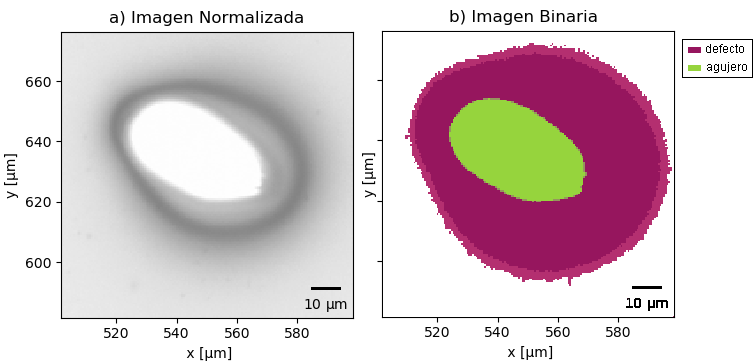
\includegraphics[scale=1.0]{Figs/cuantificaciondefectos/agujdefectocompar.png}
	\caption{\texttt{a)} Región de una imagen normalizada con el defecto más grande de la banda azul ($(81 \pm 6) \mu m$ de diámetro). \texttt{b)} Imagen binaria del defecto segmentado con el umbral original y con el umbral original modificado utilizado para cuantificar las incertezas (Ver Sección \ref{sec:incert}). }
\label{fig:deffd}
\end{figure}
 
 La falta de precisión de la normativa de \textit{scratch \& dig} dada por su método de inspección visual, la ambiguedad técnica de la determinación del \textit{scratch number} y la imposibilidad de poder caracterizar defectos con un \textit{dig number} menor a 5 (50$\mu m$), han dado lugar a la aparición de otras normativas dentro de las cuales la ISO 10110 es la más utilizada en la industria. Esta normativa indica que el control de calidad de los componentes puede ser tanto visual (con un defecto de tamaño mínimo a determinar por el fabricante) como con cualquier otro método como por ejemplo un sistema automatizado de detección como el explicado en este capítulo. De realizarse esto último como se explicó en la Sección \ref{sec:iso10110} tiene que haber un acuerdo entre el proveedor y el cliente sobre las condiciones experimentales del control de calidad que tienen que estar especificadas en la hoja de datos del componente. A continuación se explica la aplicación de la normativa ISO 10110 a los resultados del algoritmo de detección de los defectos.
 
%%%%%%%%%%%%%%%%%%%%%%%%%%%%%%%%%%%%%%%%%%%%%%%%%%%%%%%%%%%%%%%%%%%%%%%%%%%%%%%%%%%%%%%%%%%%%%%%%%%%%%%%%%%%%%%%%%%%%%%%%%%%%%%%%%%%%%%%%%%%%%%%%%%%%%%%%%%%%%%%%%%%%%%%%%%%%%%%%%%%%%%%%%%%%%%%%%%%%%%%%%%%%%%%%%%%%%%%%%%%
\singlespacing
\subsection{Aplicación de la normativa ISO 10110-7}
\label{sec:apiso}
\spacing{1.5}

\hspace{0.5cm}Como se explicó en la Sección \ref{sec:carfilt}, el fabricante no aclaró el método de inspección utilizado para garantizar la calidad óptica especificada del filtro de la normativa ISO 10110. Se va a suponer que el fabricante realizó el control de calidad vía inspección visual únicamente utilizando muestras calibradas con un mínimo \textit{grade number} igual a 0.016 (diámetro de 16 $\mu m$, ver \href{https://www.thorlabs.com/thorproduct.cfm?partnumber=MOTP-ISO}{MOTP-ISO}). Esto fue considerado de esta manera para poder aplicar los resultados del algoritmo, como fue el caso de la aplicación de la métrica de \textit{scratch \& dig}.

\begin{table}
\begin{center}
\begin{tabular}{ |c|c|c|c| }    \toprule
\texttt{Banda} & \texttt{\# de defectos} & \texttt{d$_{máx}$} & \texttt{Área$_{defectos}$}\\\midrule
\rowcolor{blue!15} Azul    & 115 & $(81 \pm 6)\mu m$ & $(71488 \pm 583)\mu m^{2}$   \\ 
\rowcolor{green!50} Verde  & 42 &  $(35 \pm 2)\mu m$ &  $(18117 \pm 248) \mu m^{2}$\\ 
Pancromática& 65 & $(51 \pm 2)\mu m$ & $(28786 \pm 61)\mu m^{2}$  \\
\rowcolor{red!50} Roja & 47 &  $(44 \pm 2)\mu m$ &   $(19798 \pm 210 )\mu m^{2}$ \\
\rowcolor{maroon!20} NIR & 44 & $(25 \pm 1) \mu m$  & $(11891 \pm 35 )\mu m^{2}$ \\
\bottomrule
 \hline
\end{tabular}
\end{center}
 \captionof{table}{Tabla de los resultados del algoritmo relevantes para la aplicación de la normativa ISO 10110. La columna $|\texttt{ \# de defectos}|$ contiene el número de defectos de diámetro mayor al mínimo \textit{grade number} considerado que es igual a 0.016 (16 $\mu m$ de diámetro máximo), considerando las incertezas.La columna  $|d_{máx}|$ indica el valor del diámetro máximo de los defectos detectado. Por último, la columna $|Área_{defectos}|$ indica el área total cubierta por los defectos de \textit{grade number} mayor a 0.016. }
 \label{tabISO}
\end{table}

De acuerdo a las especificaciones técnicas de la ISO 10110 (Ver Sección \ref{sec:iso10110}), 5/2x0.063,  en la superficie óptica de cada banda del filtro puede haber un máximo de 2 defectos de \textit{grade number} igual a 0.063 (63 $\mu m$ de diámetro)\texttt{(i)}, no puede haber defectos con un \textit{grade number} mayor a 0.063\texttt{(ii)} y, el área total máxima cubierta por defectos de \textit{grade number} mayor ó igual al mínimo valor especificado por el fabricante puede ser de 7938 $\mu m^{2}$, de acuerdo a \ref{eq:isoarea} \texttt{(iii)}. La condición \texttt{(i)} es superada por todas las bandas si se considera al defecto de diámetro máximo de la banda azul como un agujero como se discutió anteriormente y como se puede observar en los valores de la columna $|\texttt{d$_{máx}$}|$ de la Tabla \ref{tabISO} que muestran el diámetro máximo de los defectos detectados de cada banda con \textit{grade number} mayor a 0.016 ($16 \mu m$ de diámetro). Esto es así puesto que el defecto de segundo diámetro máximo detectado fue de $(52 \pm 2) \mu m$. La condición \texttt{(ii)} sería igualmente superada pero la condición \texttt{(iii)} no es superada en ninguna de las bandas como se desprende de los valores de la columna $| Área_{defectos}|$  que muestra el área cubierta por los defectos relevantes.

El método de control de calidad del filtro presentado en este capítulo podría ser compatible con el control de calidad del fabricante bajo la normativa ISO 10110. Para ello, debería establecerse un acuerdo en las condiciones experimentales bajo las que se indican las especificaciones de calidad de la superficie óptica entre las partes. Más aún, parte del presente trabajo consistió en el desarrollo de una nueva métrica para establecer qué defectos son permitidos, su tamaño máximo,etc., en función de las consecuencias que tienen los defectos en el proceso de formación de imágenes.

Por último, se hace notar que el proceso completo de detección de los defectos y de aplicación de la normativa ISO 10110 ó de la métrica de \textit{scratch \& dig} en las condiciones del método de inspección aquí propuesto, toma un tiempo total de aproximadamente 1 hora. Este tiempo estimado es resultado de considerar los 10 minutos aproximados que toma la adquisición de cada banda (50 minutos en total) y de ejecutar el procesamiento de las imágenes y el algoritmo de detección de los defectos que fue de 2 minutos por banda (10 minutos en total). En este aspecto, se hace notar que el método propuesto es lo suficientemente rápido como para no ralentizar el resto de los procesos involucrados en la construcción y puesta a punto de una cámara hiperespectral.

A continuación se muestran los resultados de la segmentación de los agujeros del filtro que permitió ubicarlos espacialmente para poder caracterizarlos espectralmente con el equipo desarrollado que se explica en el Capítulo \ref{chap:microsp}. Luego se muestran todos los defectos en general del filtro considerados detectables, de acuerdo a la resolución del microscopio y al Teorema de muestreo de Nyquist-Shannon, de un diámetro mínimo de $3 \mu m$ (Ver Sección \ref{sec:incert}). Estos resultados permitirían a futuro elegir con cierto criterio la magnificación de un microscopio a desarrollar y el tamaño del sensor de la cámara ó del diámetro de la fibra óptica de un espectrómetro del mismo equipo para determinar el área de adquisición (FOV en el caso de la cámara) y el diámetro del defecto mínimo detectable.

%%%%%%%%%%%%%%%%%%%%%%%%%%%%%%%%%%%%%%%%%%%%%%%%%%%%%%%%%%%%%%%%%%%%%%%%%%%%%%%%%%%%%%%%%%%%%%%%%%%%%%%%%%%%%%%%%%%%%%%%%%%%%%%%%%%%%%%%%%%%%%%%%%%%%%%%%%%%%%%%%%%%%%%%%%%%%%%%%%%%%%%%%%%%%%%%%%%%%%%%%%%%%%%%%%%%%%%%%%%%
\singlespacing
\subsection{Resultados del algoritmo de detección de los agujeros}
\label{sec:aguj}
\spacing{1.5}

\hspace{0.5cm} En la Tabla \ref{tabaguj} se muestran los resultados principales del algoritmo de detección de los agujeros del filtro. Como se explicó anteriormente la detección de los agujeros permitió ubicarlos espacialmente en el filtro y en consecuencia se podría caracterizar su espectro de transmisión de forma individual (Ver Capítulo \ref{chap:microsp}).

\begin{table}[H]
\begin{center}
\begin{tabular}{ |c|c|c|}    \toprule
\texttt{Banda} & \texttt{\# de agujeros} & \texttt{d$_{máx}$ agujeros} \\\midrule
\rowcolor{blue!15} Azul   & 12  & $(37 \pm 1) \mu m$  \\ 
\rowcolor{green!50} Verde  & 3 & $(11 \pm 1) \mu m$ \\ 
Pancromática & 0 & - \\
\rowcolor{red!50} Rojo  & 3 & $(9 \pm 1) \mu m$ \\
\rowcolor{maroon!20} NIR   & 1 & $(6 \pm 1) \mu m$ \\
\bottomrule
 \hline
\end{tabular}
\end{center}
 \captionof{table}{Tabla de los resultados del algoritmo de detección de los agujeros.}
 \label{tabaguj}
\end{table}

En la Figura \ref{fig:aggjj} se muestran las imágenes normalizadas originales que contienen a los agujeros más grandes de la banda NIR (\texttt{i)}) y de la banda verde (\texttt{iii}). En las imágenes \texttt{ii)} y \texttt{iv)} se muestran los resultados del algoritmo de detección de los agujeros respectivamente y se observa que el algoritmo es capaz de diferenciar a los agujeros en color verde del resto de los defectos tipo manchas en color violeta.
En la siguiente sección se muestra la población de defectos en general detectada en el filtro y luego para finalizar el capítulo se detalla la asociación de incertezas a los resultados reportados.
 \begin{figure}
\centering
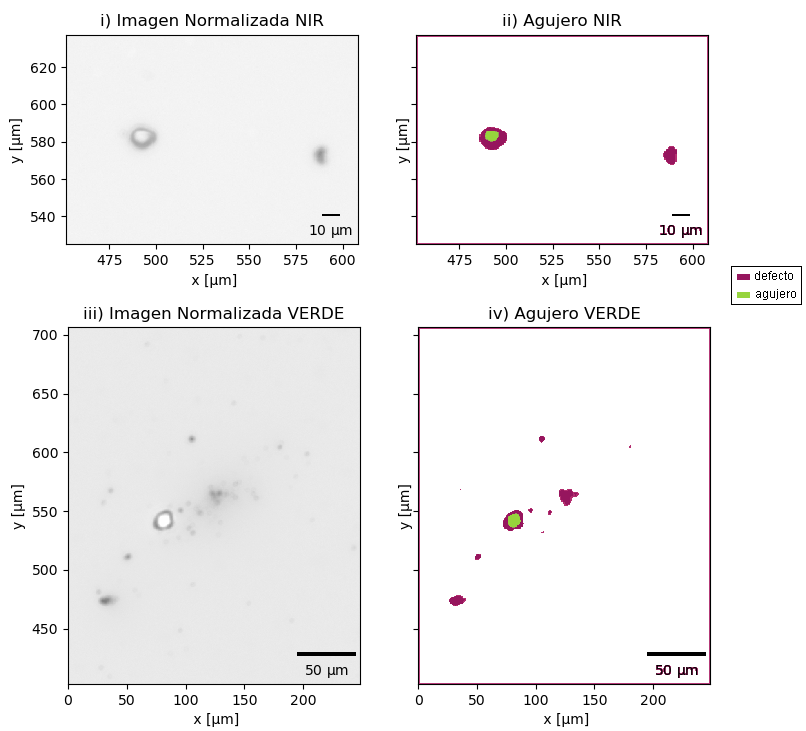
\includegraphics[scale=1.0]{Figs/cuantificaciondefectos/agujerross.png}
\caption{\texttt{i)} Imagen normalizada de la banda NIR con el agujero de diámetro máximo detectado igual a$(6 \pm 1)~ \mu m$. \texttt{ii)} Imagen binaria de la banda NIR generada a partir del algoritmo de la imagen \texttt{i)}. \texttt{iii)} Imagen normalizada de la banda verde con el agujero de diámetro máximo detectado igual a$(11 \pm 1)~ \mu m$. \texttt{iv)} Imagen binaria de la banda verde generada a partir del algoritmo de la imagen \texttt{iii)}}
\label{fig:aggjj}
\end{figure}



%%%%%%%%%%%%%%%%%%%%%%%%%%%%%%%%%%%%%%%%%%%%%%%%%%%%%%%%%%%%%%%%%%%%%%%%%%%%%%%%%%%%%%%%%%%%%%%%%%%%%%%%%%%%%%%%%%%%%%%%%%%%%%%%%%%%%%%%%%%%%%%%%%%%%%%%%%%%%%%%%%%%%%%%%%%%%%%%%%%%%%%%%%%%%%%%%%%%%%%%%%%%%%%%%%%%%%%%%%%%
\singlespacing
\subsection{Población de defectos detectados en general \href{https://github.com/jrr1984/defects\_analysis/blob/master/general\_defects\_population.ipynb}{\faGithub}}
\label{sec:defpob}
\spacing{1.5}

\hspace{0.5cm}Los resultados de esta subsección así como la determinación del diámetro de los agujeros [\ref{sec:aguj}] fueron fundamentales como criterios de elección de los componentes del equipo desarrollado que se explica en el Capítulo \ref{chap:microsp} y para el desarrollo de cualquier otro equipo alternativo.

En la Tabla \ref{tabpobb} se muestran los resultados representativos y cuantitativos de la población de defectos en general detectados de diámetro mayor a los $3\mu m$ incluyendo a los agujeros.

\begin{table}[H]
\begin{center}
\begin{tabular}{ |c|c|c|c|c|c|}    \toprule
\texttt{Banda} &  \texttt{\# defectos} & \texttt{d$_{máx}$ defectos} & \texttt{\% Área$_{defectos}$} & \texttt{\# agujeros} & \texttt{d$_{máx}$ agujeros} \\\midrule
\rowcolor{blue!15} Azul   & 5443 & $(81 \pm 6) \mu m$ & 0.14 \% &12  & $(37 \pm 1) \mu m$  \\ 
\rowcolor{green!50} Verde  & 2209 & $(35 \pm 2) \mu m$ & 0.07 \% &3 & $(11 \pm 1) \mu m$\\ 
Panc. & 2065 & $(51 \pm 2) \mu m$ & 0.09 \% &0 & -\\
\rowcolor{red!50} Rojo  & 1405  &$(44 \pm 2) \mu m$& 0.06 \% &3 & $(9 \pm 1) \mu m$\\
\rowcolor{maroon!20} NIR   & 1552 & $(25 \pm 1) \mu m$ & 0.04 \% &1 & $(6 \pm 1) \mu m$ \\ \midrule
Total   & 12674 & $(81 \pm 6) \mu m$ & 0.08 \% & 19 & $(37 \pm 1) \mu m$ \\
\bottomrule
 \hline
\end{tabular}
\end{center}
 \captionof{table}{Tabla de los resultados representativos del algoritmo de detección de los defectos. La columna $| \texttt{\# de defectos}|$ muestra el número de defectos de diámetro mayor a $3 \mu m$. Este diámetro mínimo fue elegido considerando la resolución del microscopio y el Teorema de muestreo de Nyquist-Shannon (Ver Sección \ref{sec:incert}). La columna $|\texttt{d$_{máx}$ defectos}|$ indica el diámetro máximo de los defectos detectados. La columna $|\texttt{\% Área$_{defectos}$}|$ indica el porcentaje aproximado del área total de cada banda cubierta por defectos. El área total de cada banda considerada fue igual al área adquirida en el \textit{tile scan}. La fila $|$Tota$l|$ resume los resultados de las cinco bandas: número total de defecto, diámetro máximo de los defectos detectados, porcentaje de área total (de la suma de las áreas de las 5 bandas) cubierta por los defectos, número de agujeros y diámetro máximo de los agujeros detectados.}
 \label{tabpobb}
\end{table}

Se hace notar que resulta inevitable que entre los defectos detectados haya partículas de polvo y otras suciedades en general dado que esta inspección no fue realizada en una sala limpia.  Ahora bien, si el método propuesto en este capítulo se desarrollara industrialmente, la Tabla \ref{tabpobb} podría ser incluida en una hoja de datos del filtro y a partir de su análisis se podría determinar bajo algún criterio a desarrollar en conjunto con el proveedor, si el filtro supera las especificaciones de calidad propias de la aplicación en cámaras hiper y multiespectrales utilizadas en satélites. 

En la Figura \ref{fig:boxpl} se muestra el \textit{boxplot} (también llamado \textit{box-and-whisker plot}) de la distribución de los valores del diámetro de los defectos. La mediana de dicha distribución, es decir el valor del percentil 50, fue igual a $4\mu m$, lo que indica que el 50\% de los defectos tuvieron un diámetro menor a $4 \mu m$. El percentil 75 fue igual a $5 \mu m$, es decir que el 75\% de los defectos detectados fueron de un diámetro menor a $5 \mu m$.

\begin{figure}
\centering
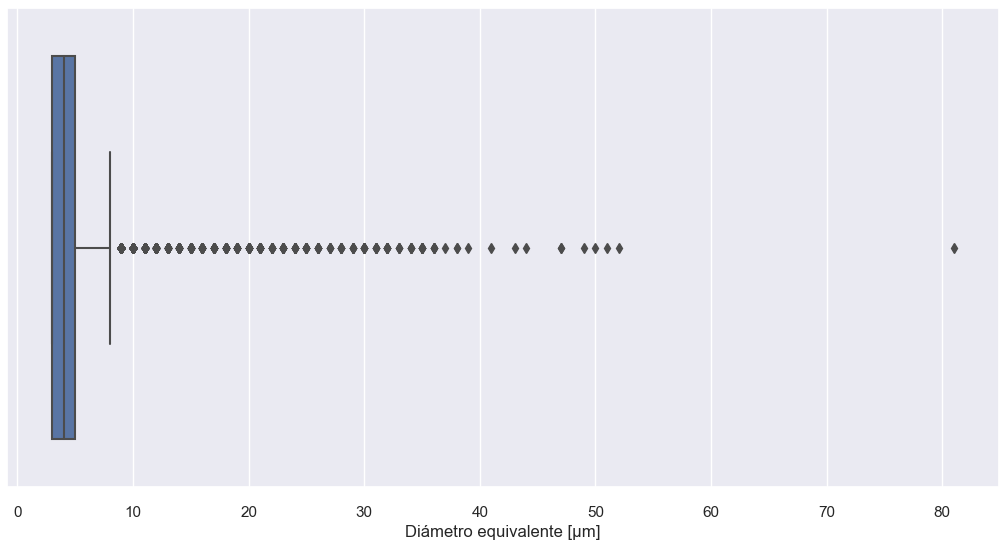
\includegraphics[scale=0.9]{Figs/cuantificaciondefectos/boxplotdefectos.png}
\caption{Boxplot del diámetro de los defectos de diámetro mayor ó igual a 3 $\mu m$.}
\label{fig:boxpl}
\end{figure}

A partir de los resultados de la distribución del diámetro de los defectos, se decidió diseñar el microespectrómetro que se explica en el Capítulo \ref{chap:microsp} con una resolución óptica lateral capaz de detectar defectos de diámetro mínimo igual a 20$\mu m$, es decir que se decidió caracterizar a la gran mayoría de los defectos que aparecen como \textit{outliers} en el boxplot de la Figura \ref{fig:boxpl}. Los \textit{outliers} son todos los defectos de diámetro mayor al valor del cuarto percentil de la muestra de los datos y que en el gráfico está indicado por la barra vertical a la derecha del \textit{box}.

En la última sección de este capítulo se explica cómo se asociaron las incertezas a los diámetros y áreas de los defectos y agujeros detectados.

%%%%%%%%%%%%%%%%%%%%%%%%%%%%%%%%%%%%%%%%%%%%%%%%%%%%%%%%%%%%%%%%%%%%%%%%%%%%%%%%%%%%%%%%%%%%%%%%%%%%%%%%%%%%%%%%%%%%%%%%%%%%%%%%%%%%%%%%%%%%%%%%%%%%%%%%%%%%%%%%%%%%%%%%%%%%%%%%%%%%%%%%%%%%%%%%%%%%%%%%%%%%%%%%%%%%%%%%%%%%
\singlespacing
\section{Asociación de incertezas a los resultados del algoritmo}
\label{sec:incert}
\spacing{1.5}

\hspace{0.5cm} El diámetro mínimo de un defecto detectable debe ser, de acuerdo al Teorema de Nyquist-Shannon, mayor ó igual que el doble del poder de resolución(R) del microscopio que viene dado por el Criterio de Rayleigh (fuente de luz incoherente) y que es igual a:
\begin{equation}
R = \frac{0.61 \hspace{2pt} \lambda}{ N.A.},
\label{eq:rayleighcrit}
\end{equation}
donde $\lambda$ es la longitud de onda central de la fuente de luz utilizada, que en este caso fue una fuente de luz blanca por lo que considerando $\lambda = 0.55 \mu m$. y, N.A. es la apertura numérica del objetivo que fue de 0.25. En consecuencia, la resolución óptica del microscopio estimada teóricamente fue de 1.34$\mu m$\footnote{Si se considera que la fuente de luz tuvo un espectro de emisión en el rango con longitudes de onda entre 400 y 700 nm, la resolución teórica estimada se encuentra en el rango comprendido entre los 0.98 y 1.71 $\mu m$.}. De esta manera el diámetro del mínimo defecto detectable fue igual a 2 x 1.34$\mu m = 2.68 \mu m \sim 3 \mu m$, donde se aproximó el resultado puesto que se trata de un límite teórico y para establecer la precisión de todos los resultados adquiridos con el algoritmo. De acuerdo a la calibración del microscopio cada píxel equivale a 0.586$\mu m$, con lo cual el diámetro del defecto más chico detectable medido en cantidad de píxeles fue de 5 píxeles (5 x 0.586$\mu m$ = 2.94$\mu m \sim$ 3$\mu m$). Este criterio se implementó en el algoritmo por medio del método \textit{morphology.remove\_small\_objects} eligiendo el tamaño del mínimo defecto a detectar en el argumento \textit{min\_size} de la función.

El error principal del algoritmo en la detección de los defectos y en consecuencia en la determinación del diámetro equivalente  y área de los mismos consistió en la precisión con la que se determinó el borde de cada defecto. Esto último depende fuertemente del grado de contraste de la transición de los valores de intensidad en la imagen desde el borde del defecto hasta el fondo de la imagen que lo rodea \cite{quentin}. Para cuantificar este error se realizó una variación del umbral de intensidad que distinguía a los defectos del fondo de la imagen. La variación del valor del \textit{threshold} fue de hasta el 8\% del valor del \textit{threshold} original dependiendo de cada banda. A partir del valor de umbral modificado, el proceso de segmentación y determinación de las propiedades de los defectos resultó el mismo que con el valor de umbral original. El criterio de elección del porcentaje de variación del umbral consistió en que se tenía que obtener la misma cantidad de defectos que con el umbral original de forma tal de poder calcular el error de forma automatizada. Esto al mismo tiempo aseguraba que dicha variación no fuera tan grande como para que el algoritmo no pudiera segmentar dos defectos muy cercanos ó por otro lado dejar de detectar ciertos defectos. En la Figura \ref{fig:bordedefe} se muestra una región con un defecto de la banda verde (Imagen \texttt{a)}) y las imágenes binarias del \textit{threshold} original y de su variación superpuestas (Imagen \texttt{b)}). En la Imagen \texttt{c)} de la misma figura se muestra un \textit{zoom} sobre uno de los bordes del defecto donde los píxeles de color rosa están asociado a la imagen binaria generada con el \textit{threshold} original y los píxeles de color violeta están asociados a la variación de dicho umbral.
\begin{figure}
\centering
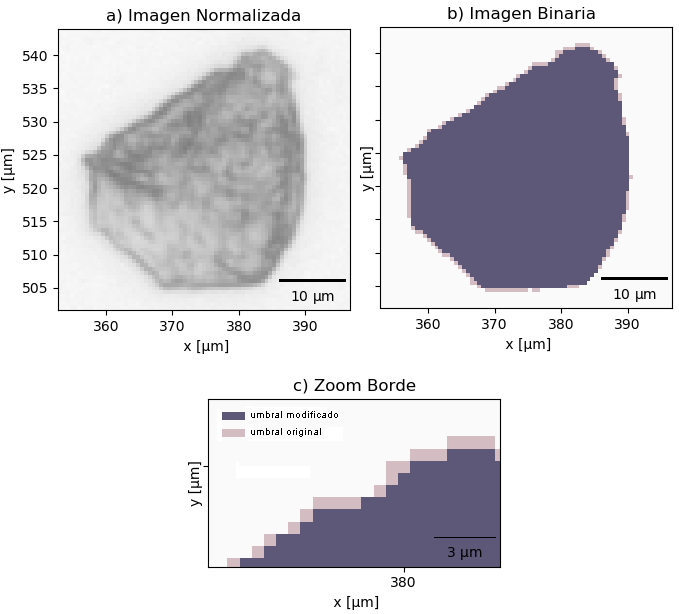
\includegraphics[scale=1.1]{Figs/cuantificaciondefectos/erroresborde.png}
\caption{\texttt{a)} Región de una imagen normalizada con un defecto de la banda verde.\texttt{b)} Imágenes binarias superpuestas del umbral original y de su variación para cuantificar el error cometido. \texttt{c)} Zoom sobre uno de los bordes del defecto.}
\label{fig:bordedefe}
\end{figure}

En el ejemplo de la Figura \ref{fig:bordedefe} se obtuvo un defecto con un área que para el umbral original estuvo compuesta por 2793 píxeles (959$\mu m^{2}$) y para su variación el área fue de 2640 píxeles (906$\mu m^{2}$). El diámetro equivalente fue de 35$\mu m$ y 34$\mu m$ respectivamente. En todos los resultados de diámetros y áreas de defectos detectados con el algoritmo explicado en la sección \ref{sec:secalg}, se reportó el resultado obtenido con el umbral original y se asoció como incerteza la diferencia entre el valor obtenido con el umbral y su variación. Así por ejemplo, el defecto de la Figura \ref{fig:bordedefe} tuvo un diámetro de $(35 \pm 1) \mu m$.

A continuación se describe la construcción y montaje del equipo desarrollado para caracterizar espectralmente a los defectos definidos en este capítulo como agujeros ó huecos (Ver Figura  \ref{fig:huecoazul}) y manchas ó defectos de transmisión (Ver Figura \ref{fig:manchaazul}).

\singlespacing
\chapter{Diseño, construcción y aplicación de un microespectrómetro}
\label{chap:microsp}
\spacing{1.5}

\hspace{0.5cm}En el Capítulo \ref{chap:zeiss} se realizó un análisis cuantitativo de los defectos de filtros multiespectrales de cámaras de satélites: se determinó su área, su diámetro equivalente, etcétera. Dicho análisis permitió aplicar las especificaciones técnicas de \textit{scratch \& dig} y de la ISO 10110, lo que resulta fundamental para establecer las bases de futuros acuerdos con los fabricantes de los componentes ópticos. Al mismo tiempo, los resultados de la población de defectos [\ref{sec:defpob}] detectados con el algoritmo, permitieron establecer los criterios de diseño óptico del microespectrómetro que se explica en el presente capítulo.

Como se explicó en la Sección \ref{sec:microespp}, un microespectrómetro es un instrumento de medición híbrido que integra la capacidad de magnificación y de resolución ópticas de un microscopio con la capacidad de inferir las propiedades espectrales de un material. En este capítulo se describe el diseño y la construcción de un microespectrómetro que permitió realizar una caracterización del filtro y de sus defectos a través de los espectros de transmisión. En la Sección \ref{sec:prot0} se muestran las características del primer prototipo desarrollado con equipamiento disponible en el laboratorio. Dicho prototipo en conjunto con los resultados y análisis del Capítulo \ref{chap:zeiss}, permitieron establecer los criterios de elección de la fuente de luz y del espectrómetro [\ref{sec:fteluzyesp}], determinar la longitud del recorrido y la precisión mínima necesaria de la platina que se desarrolló [\ref{sec:platina}] y la resolución óptica necesaria del microscopio desarrollado para caracterizar los defectos de diámetro mayores a 20 $\mu m$ de diámetro. Luego se explica el proceso de montaje y alineación preliminar del microespectrómetro [\ref{sec:montalin}]. Posteriormente se explica la integración de una cámara \textit{web} al microespectrómetro lo que permitió la adquisición simultánea de imágenes digitales y de espectros de transmisión y cuya área de adquisición fue elegida con un \textit{joystick} y visualizada en vivo a través de una interfaz gráfica [\ref{sec:camwebgui}]. Luego se detalla la caracterización del microespectrómetro [\ref{sec:caractequipo}], su puesta en foco y la determinación de la resolución espacial [\ref{sec:focoresol}, \ref{sec:fococam}].

Asimismo, se muestra la aplicación del microespectrómetro a la caracterización espectral del filtro y de sus defectos [\ref{sec:resgrales}]. Se describen los resultados de los espectros de transmisión de cada banda del filtro y su comparación con la hoja de datos reportada por el fabricante [\ref{sec:espectransm}]. Finalmente, se muestran los resultados de la caracterización espectral de los defectos denominados manchas ó defectos de transmisión [\ref{sec:defctma}] y de los agujeros ó huecos [\ref{sec:defctag}].

%%%%%%%%%%%%%%%%%%%%%%%%%%%%%%%%%%%%%%%%%%%%%%%%%%%%%%%%%%%%%%%%%%%%%%%%%%%%%%%%%%%%%%%%%%%%%%%%%%%%%%%%%%%%%%%%%%%%%%%%%%%%%%%%%%%%%%%%%%%%%%%%%%%%%%%%%%%%%%%%%%%%%%%%%%%%%%%%%%%%%%%%%%%%%%%%%%%%%%%%%%%%%%%%%%%%%%%%%%%%

\singlespacing
\section{Prototipo preliminar \href{https://github.com/jrr1984/Prototipo0\_S-D\_SpectralGUI}{\faGithub}}
\label{sec:prot0}
\spacing{1.5}

\hspace{0.5cm}El desarrollo del prototipo preliminar que se muestra en esta sección permitió establecer los criterios de elección de la fuente de luz y el recorrido y la precisión necesarias de la platina desarrollada para poder adquirir el espectro e imágenes del filtro completo. Como buena práctica de prototipado de instrumentos de medición se utilizaron componentes y equipamiento disponibles en el laboratorio, es decir que no se incurrió en gastos adicionales de dinero a excepción del costo del material de las impresiones 3D del soporte del filtro. Por otro lado, a partir del desarrollo del software automatizado de adquisición y de visualización de los resultados de este prototipo se establecieron las características deseadas y esperadas del prototipo final desarrollado. De esta manera, el prototipo permitió establecer la factibilidad del desarrollo del equipo.

Como objetivo general se propuso desarrollar un sistema integral de caracterización de filtros ópticos de interferencia utilizados en cámaras hiper y multiespectrales. Inicialmente se establecieron tres objetivos específicos:
\begin{enumerate}
\item Desarrollar un sistema automatizado de adquisición del espectro de transmisión de cada una de las bandas del filtro.$\xrightarrow{}$ \href{https://github.com/jrr1984/Prototipo0\_S-D\_SpectralGUI/blob/master/barrido/std}{\faGithub}

\item Determinar un mapa multiespectral ($\textit{x}$,$\textit{y}$,$\lambda$) del filtro.$\xrightarrow{}$ \href{https://github.com/jrr1984/Prototipo0\_S-D\_SpectralGUI/blob/master/spectral\_gui/main.py}{\faGithub}

\item Integrar un sistema de detección y caracterización de los defectos del filtro.
\end{enumerate}

A continuación se describen los primeros dos objetivos que fueron abarcados por el prototipo preliminar descripto en esta sección. Respecto del primer objetivo, se montó el arreglo experimental que se muestra en las Figuras \ref{fig:setup0}, \ref{fig:setup01} y \ref{fig:setup02}. 

\begin{figure}[H]
	\centering
	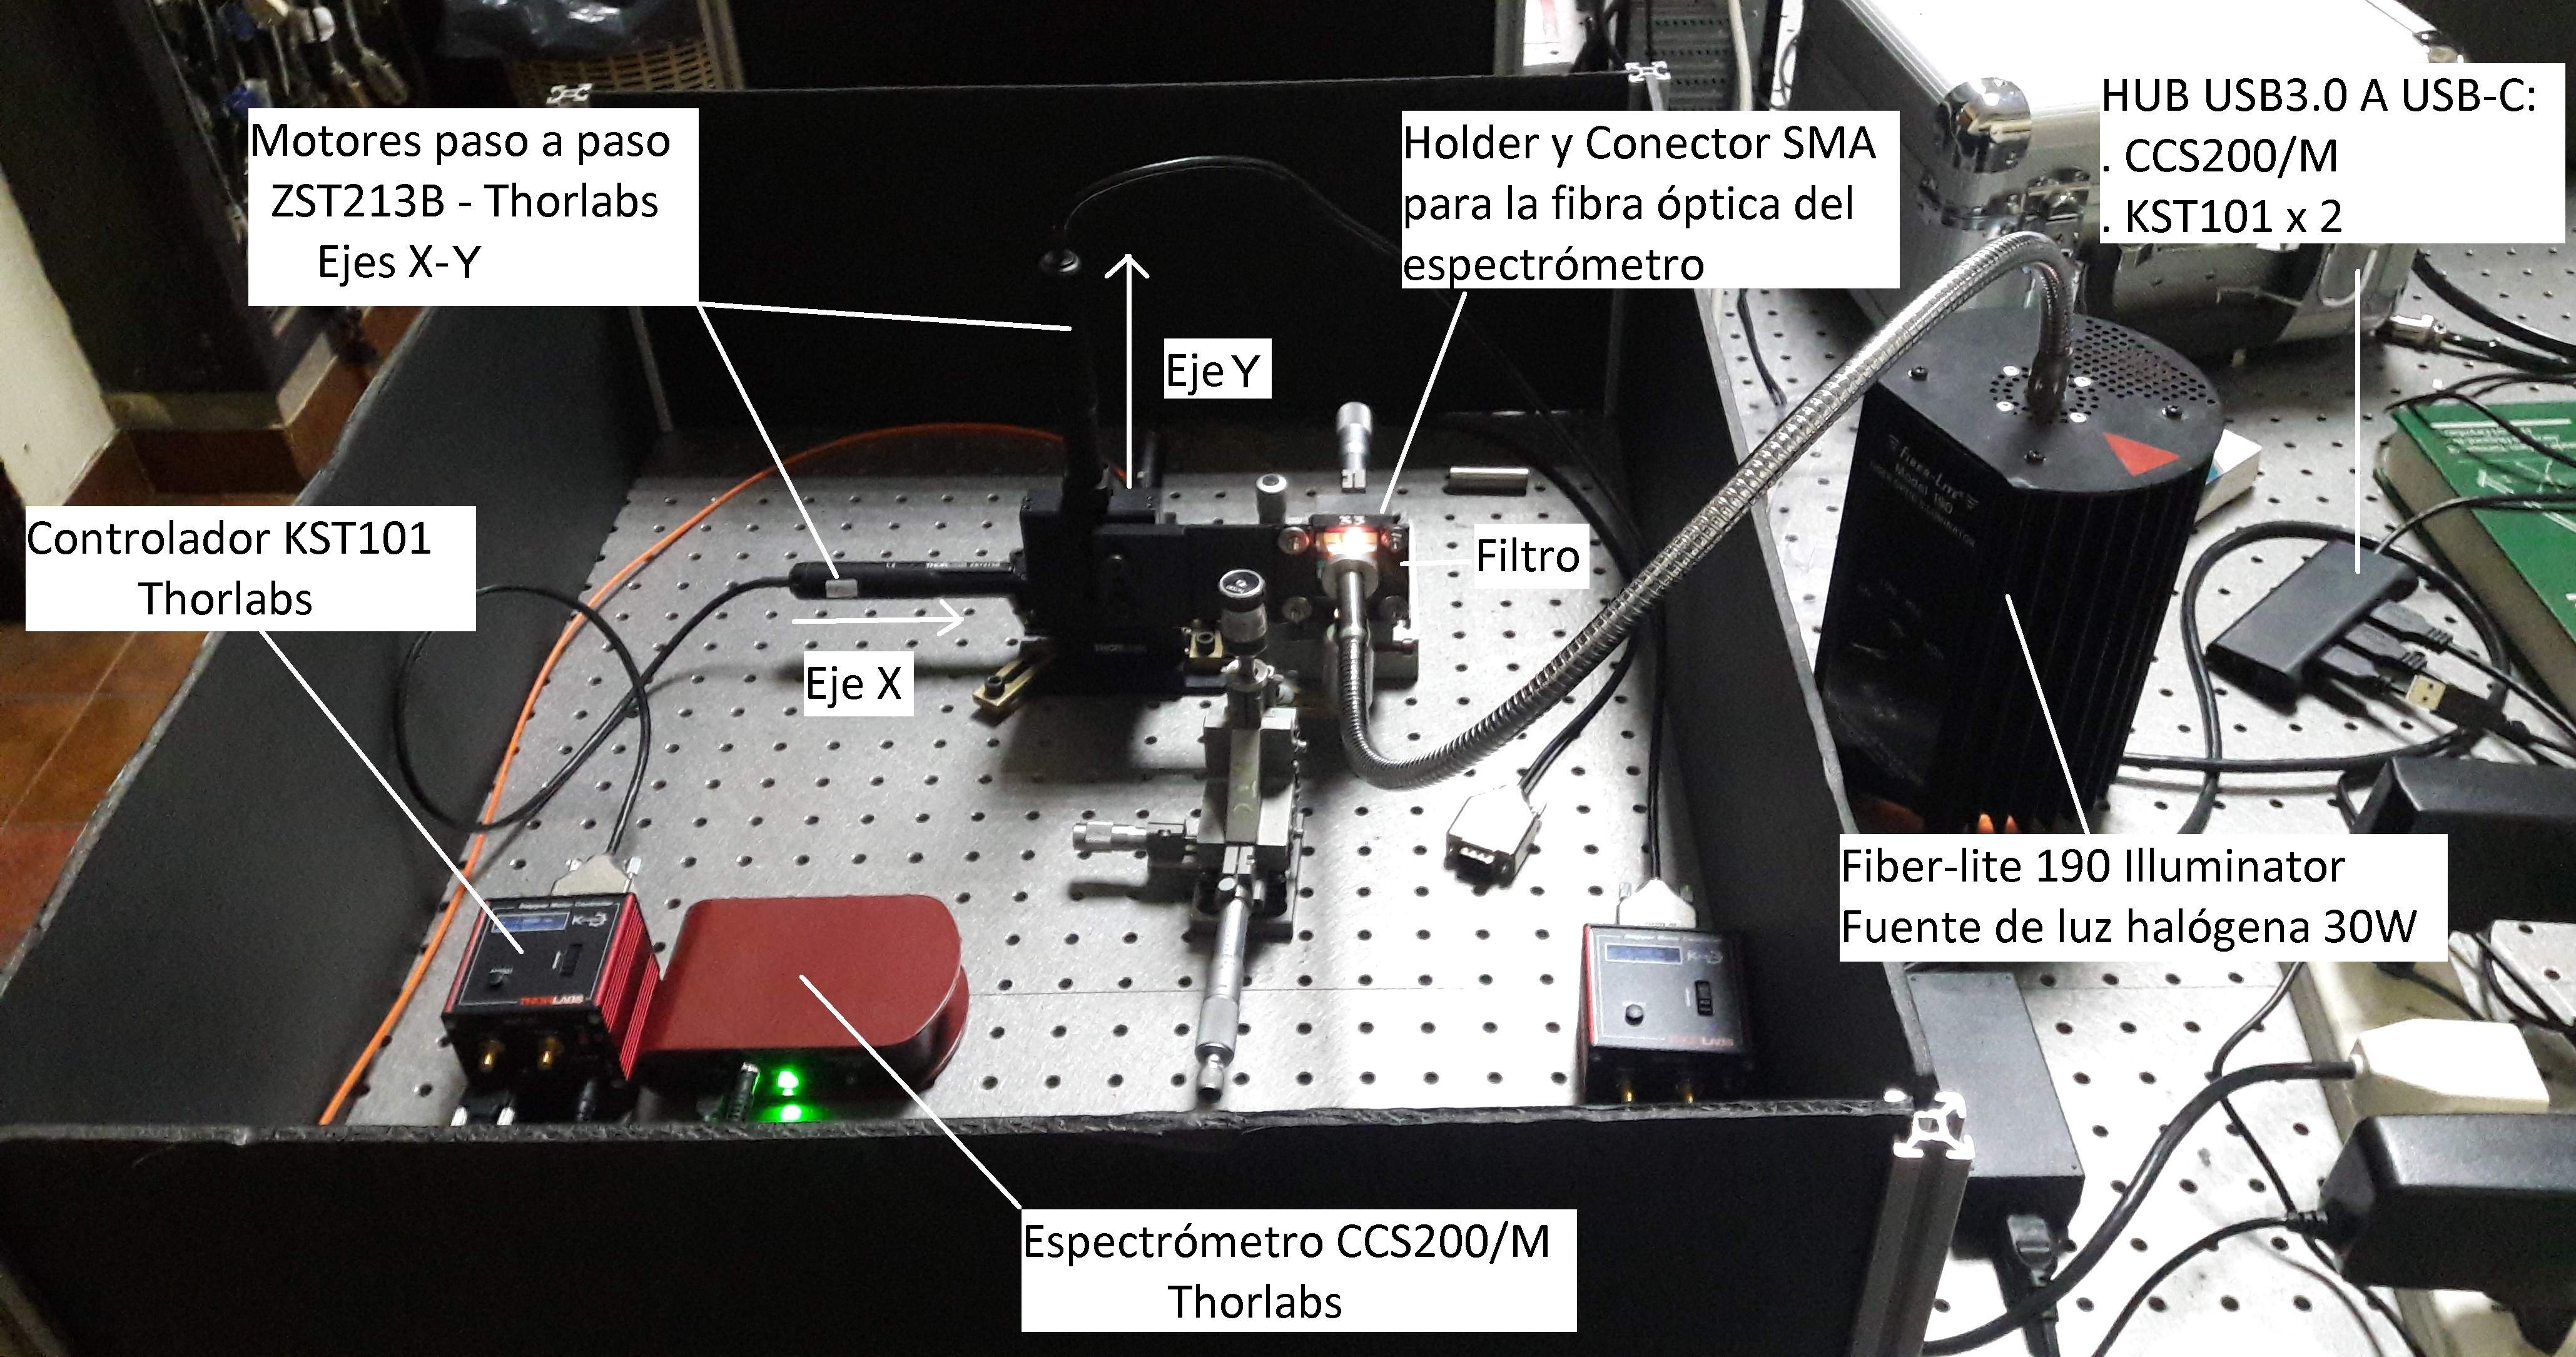
\includegraphics[width=1.0\textwidth]{Figs/microespectrometro/setupbarridooriginal.jpg}
	\caption{Arreglo experimental del prototipo preliminar.}
	\label{fig:setup0}
\end{figure}

\begin{figure}[H]
	\begin{floatrow}
		\ffigbox{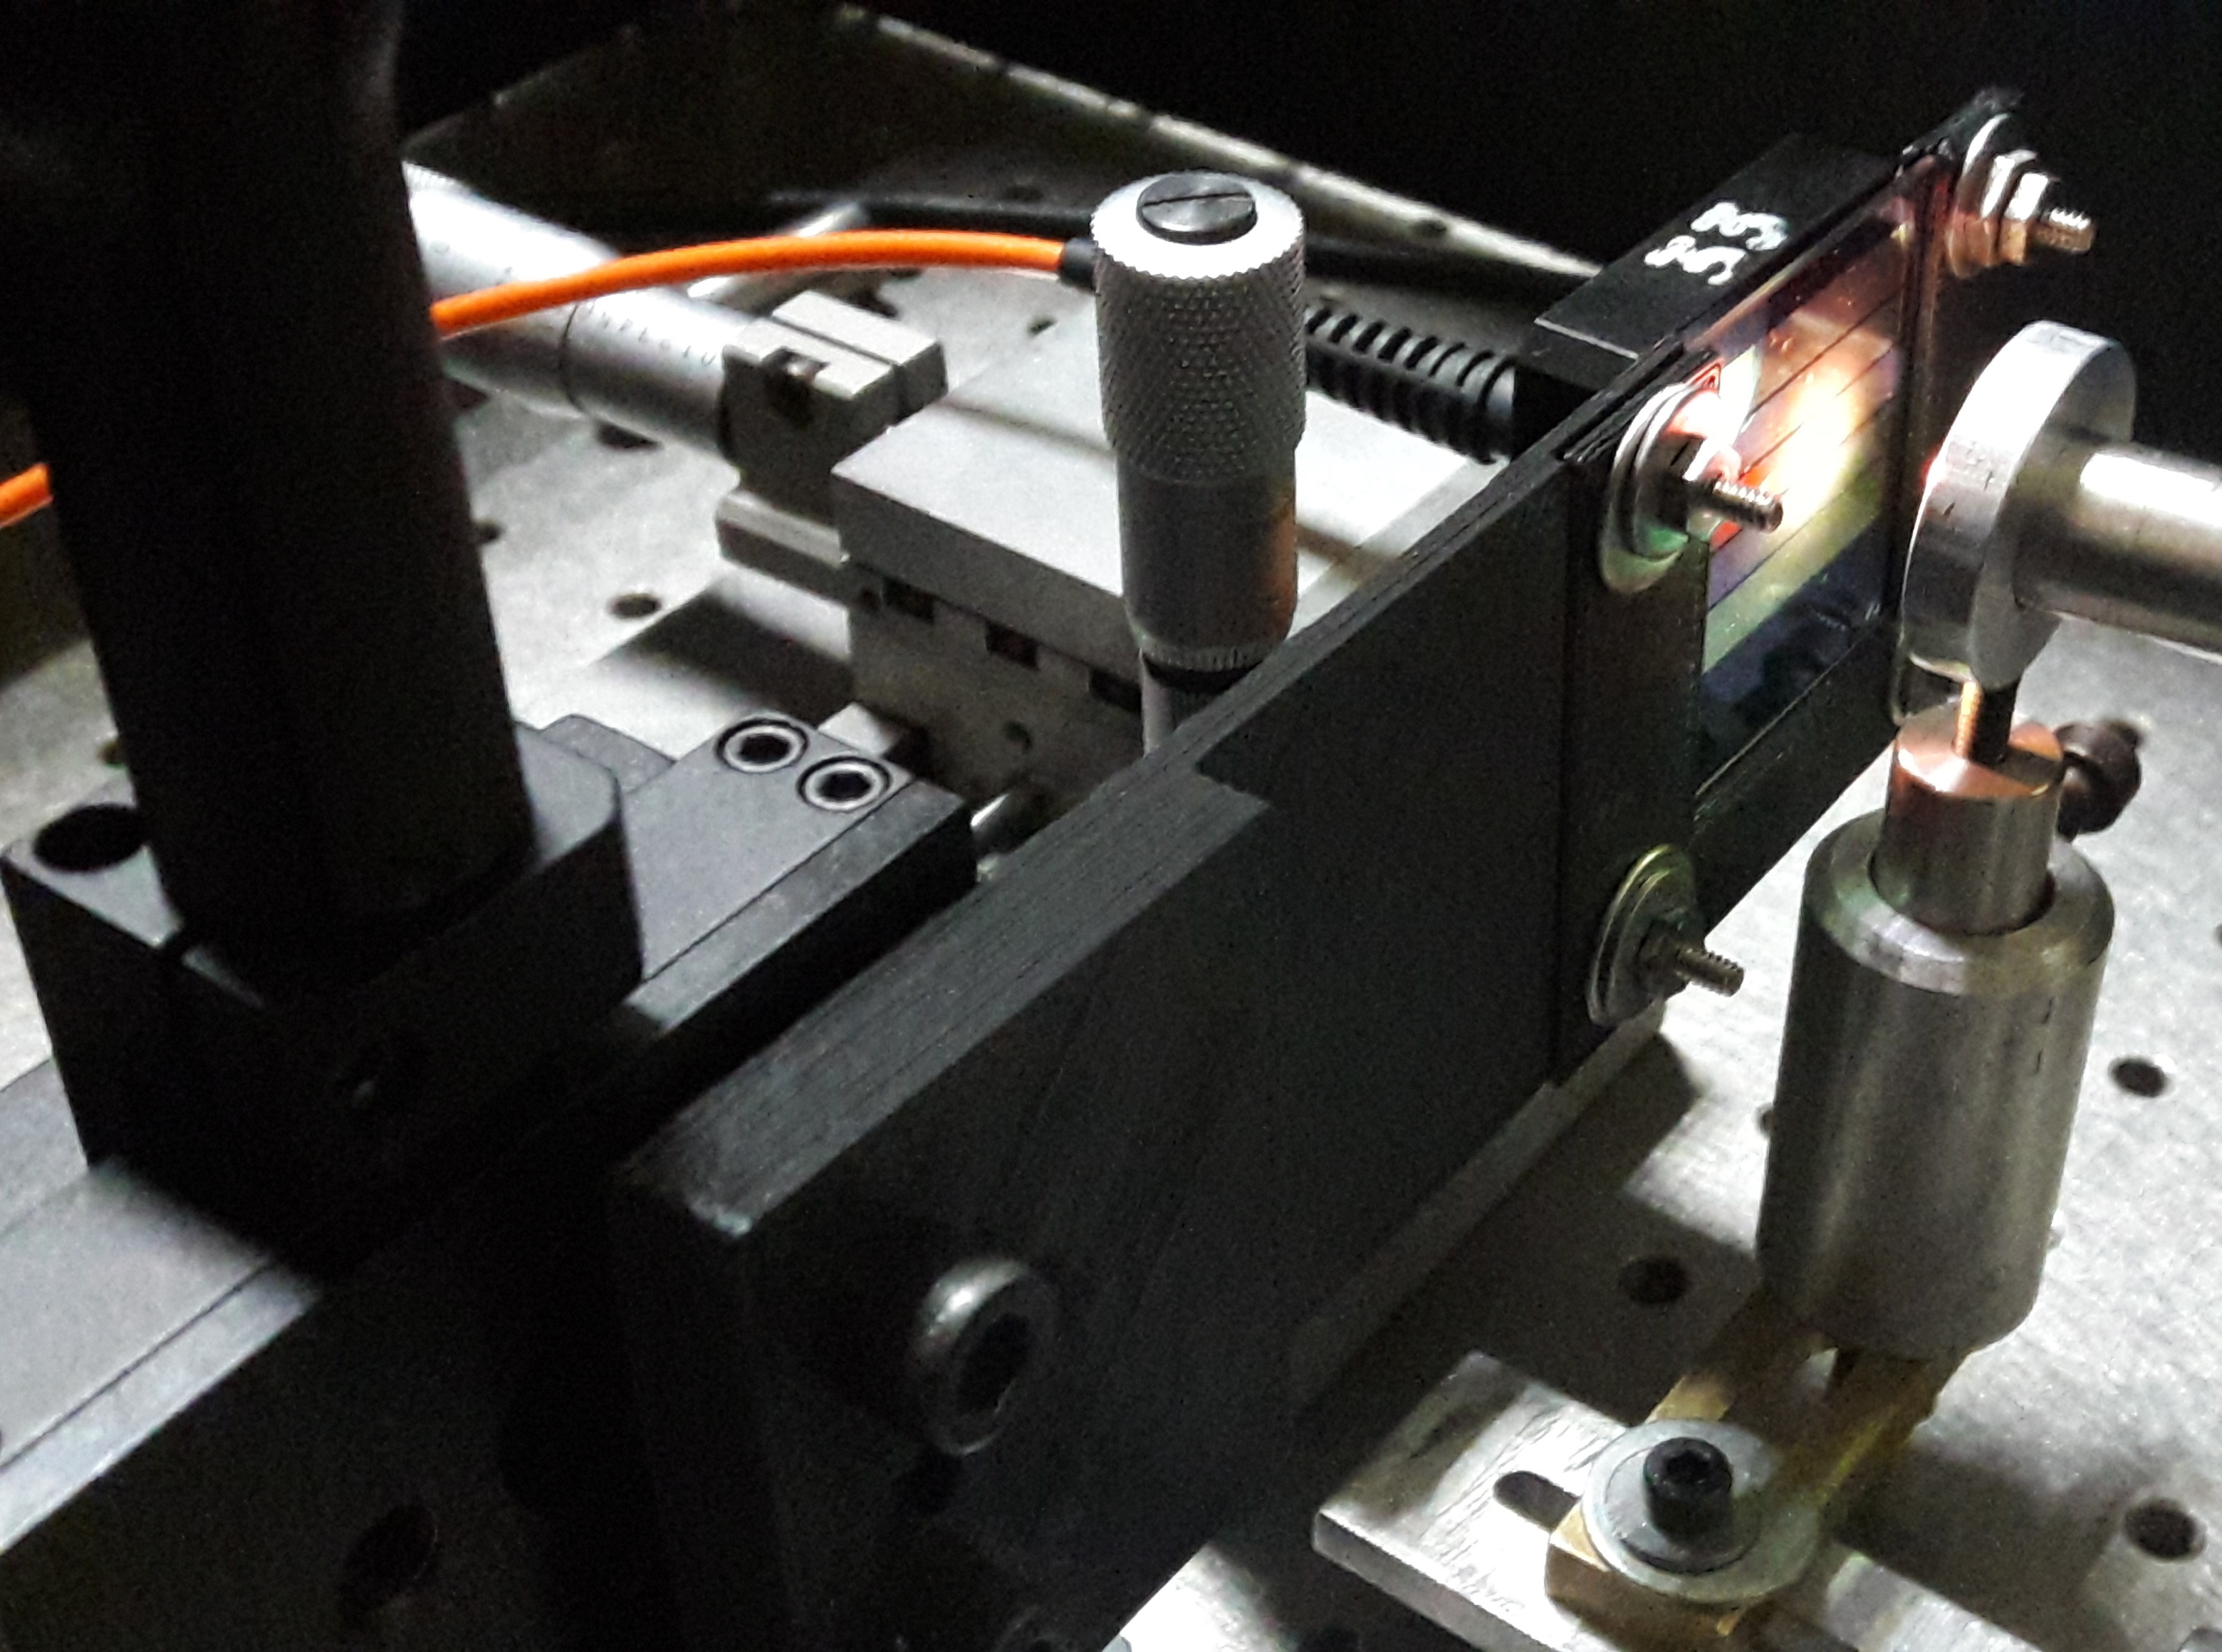
\includegraphics[scale=0.073]{Figs/microespectrometro/montajesetup0.jpg}}{\caption{Vista lateral del montaje del filtro sobre el soporte que se encuentra atornillado con unos tornillos M6 a la plataforma motorizada de Thorlabs.}\label{fig:setup01}}
		\ffigbox{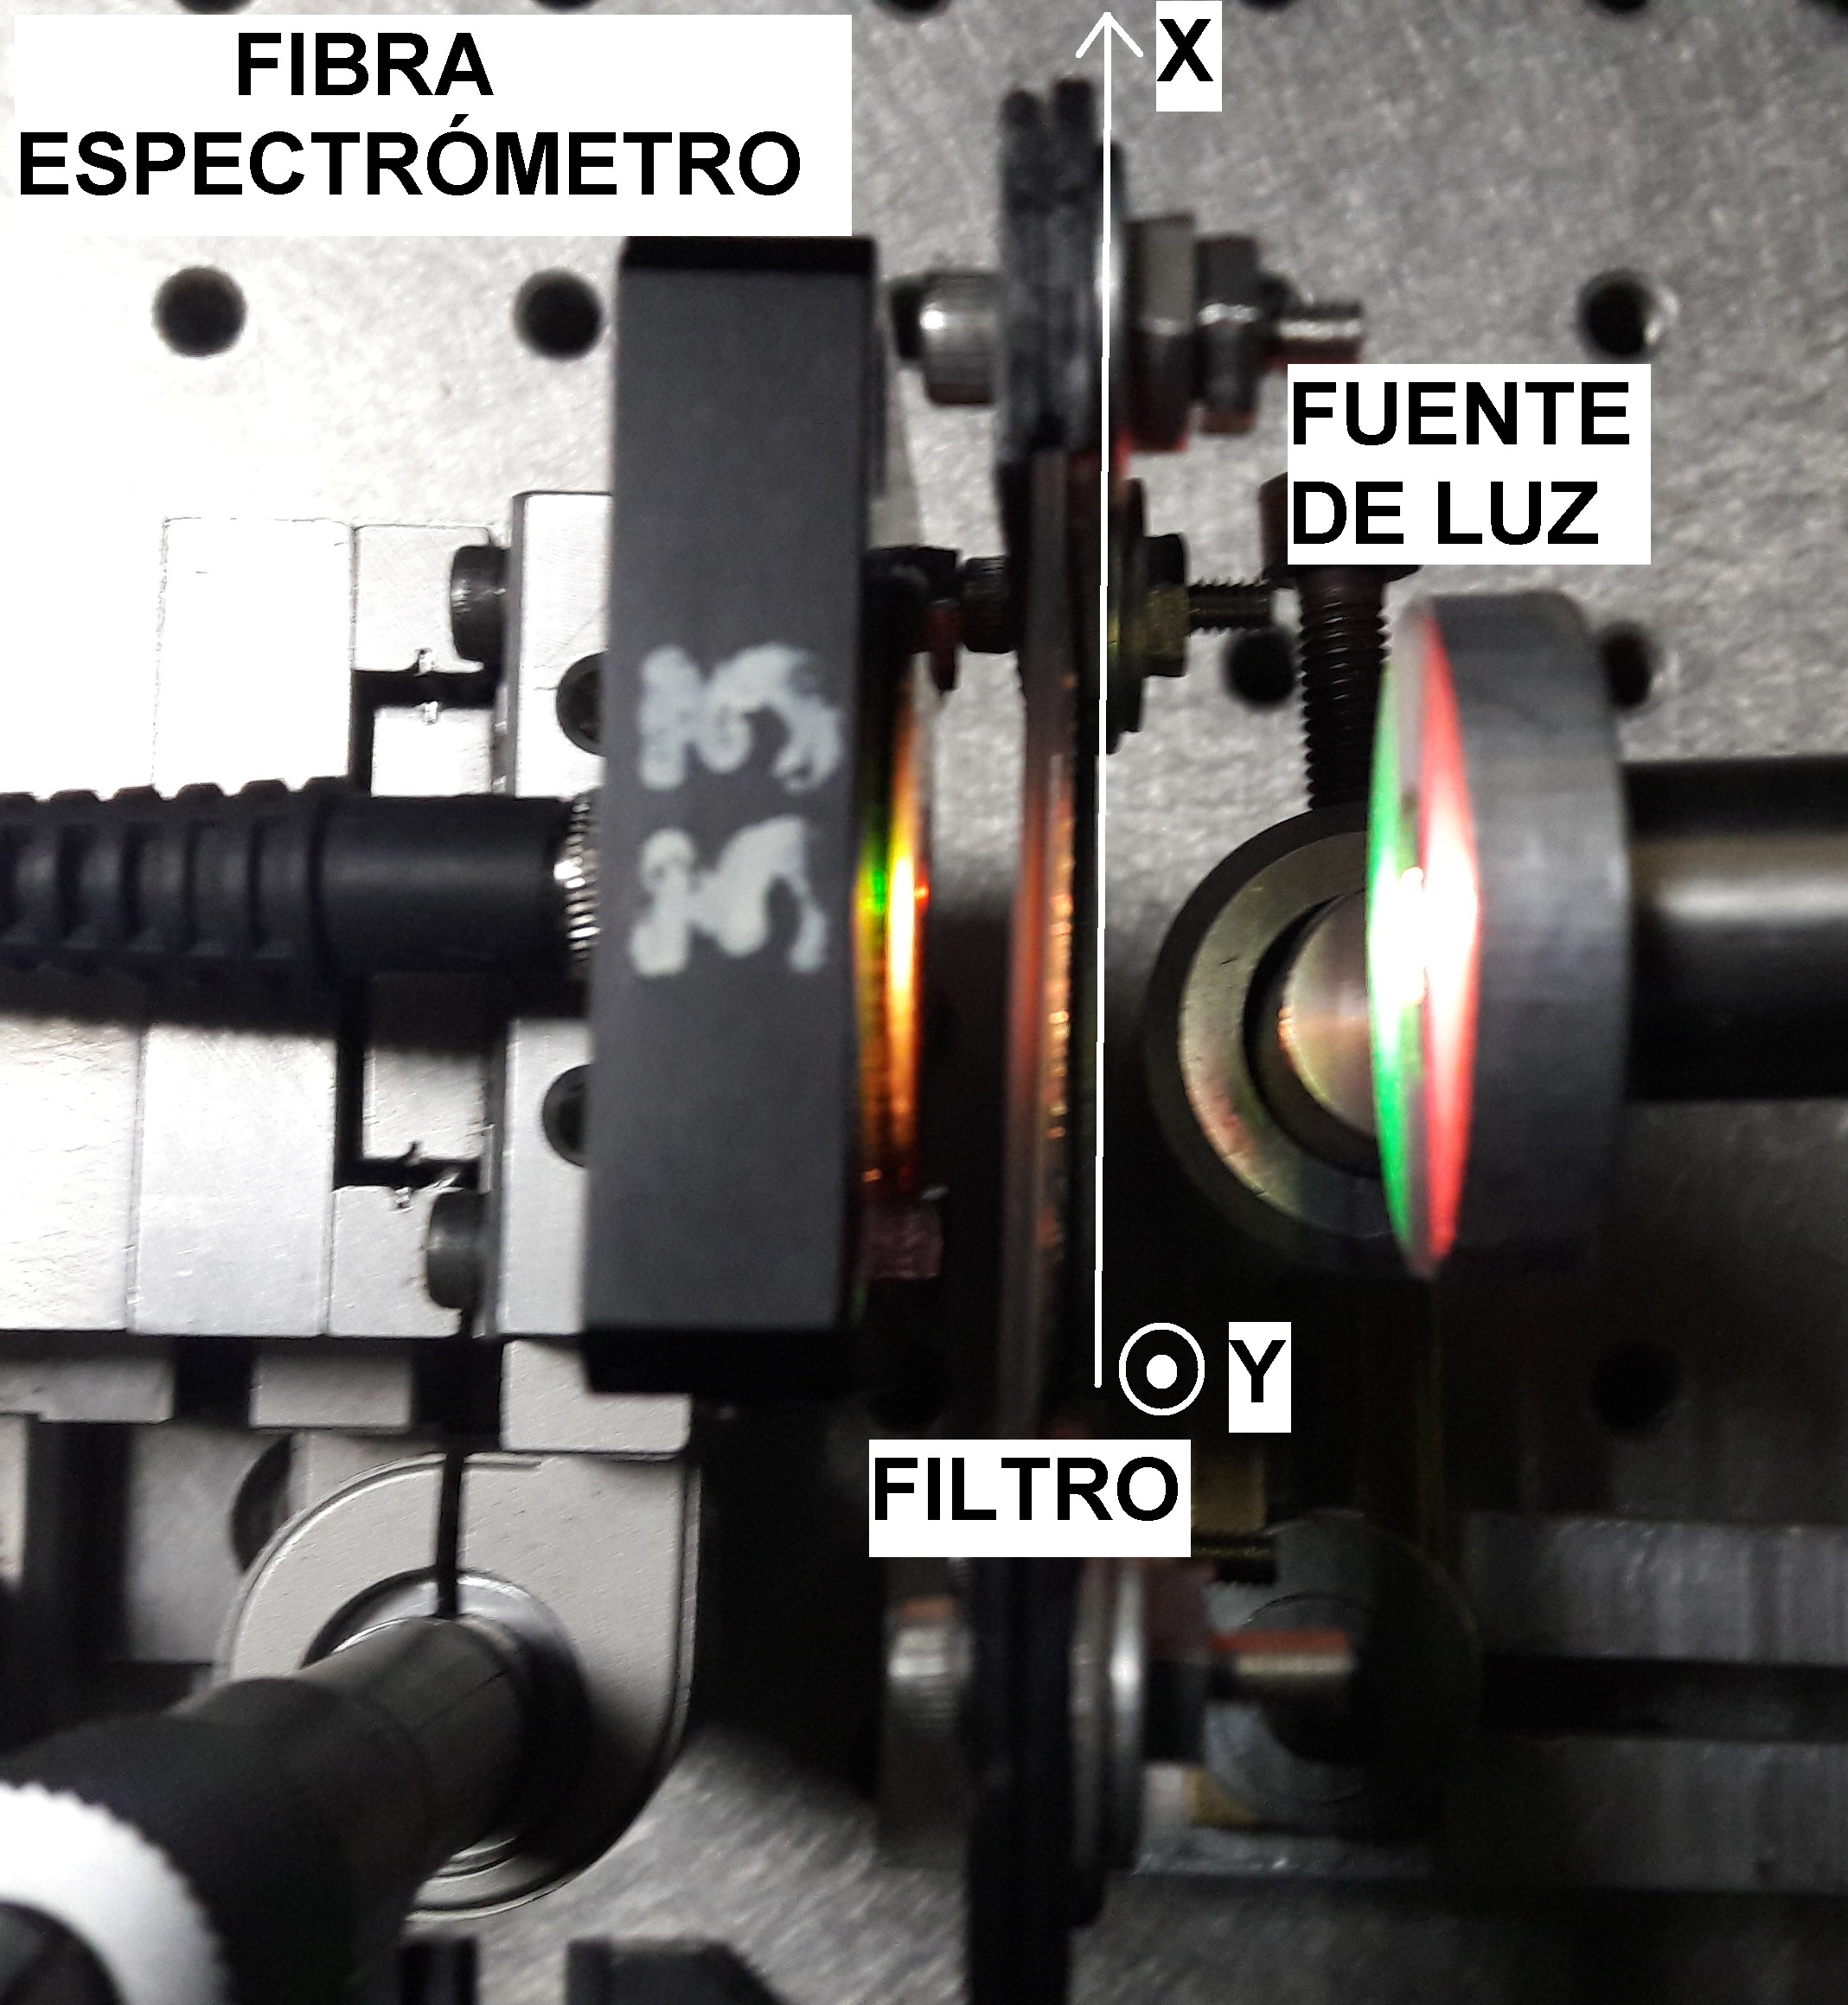
\includegraphics[scale=0.073]{Figs/microespectrometro/5.jpg}}{\caption{El filtro se mueve en los ejes $\textit{x}$ e $\textit{y}$ definidos en la imagen, de forma perpendicular a la incidencia de la luz que define el eje z denominado óptico en adelante. }\label{fig:setup02}}
	\end{floatrow}
\end{figure}

Con una fuente de luz halógena, modelo \href{https://dolan-jenner.com/products/fiber-lite-190}{\textit{Fiber-lite 190 Illuminator}}, se incidió perpendicularmente sobre el filtro y su transmisión fue detectada por la fibra óptica de un espectrómetro modelo \href{https://www.thorlabs.com/thorproduct.cfm?partnumber=CCS200/M#ad-image-0}{CCS 200/M} de la empresa Thorlabs (\textit{Driver} de \textit{python}: \href{https://github.com/jrr1984/Prototipo0\_S-D\_SpectralGUI/blob/master/syst/CCS200.py}{\faGithub}). De la misma manera en que se realizó el \textit{Tile Scan} del filtro completo con el microscopio Zeiss explicado en la sección \ref{subs:tilsc} (Ver Figura \ref{fig:tilescan}), se desplazó el filtro a lo largo del eje x, barriendo en `filas' y realizando el desplazamiento vertical en los extremos del máximo recorrido de los tornillos accionados por los motores paso a paso que fue de 13 mm. Dicho desplazamiento fue realizado con una plataforma de tres grados de libertad, modelo \href{https://www.thorlabs.com/thorproduct.cfm?partnumber=MT3/M}{MT3/M} de la empresa Thorlabs, cuyos tornillos micrométricos fueron intercambiados por unos motores paso a paso modelo \href{https://www.thorlabs.com/thorproduct.cfm?partnumber=ZST213B}{ZST213B} cuyos controladores de corriente fueron también de la empresa Thorlabs, modelo \href{https://www.thorlabs.com/thorproduct.cfm?partnumber=KST101}{KST101} (\textit{Driver} de \textit{python}: \href{https://github.com/jrr1984/Prototipo0\_S-D\_SpectralGUI/blob/master/barrido/std/thor\_stepm.py}{\faGithub}). Como las dimensiones de la región comprendida por las cinco bandas del filtro es de 27 mm x 25 mm, con esta plataforma no se pudo realizar una adquisición del filtro completa en una sola configuración como la propuesta. El \textit{software} automatizado de adquisición del espectro de transmisión del filtro desarrollado para este prototipo [\href{https://github.com/jrr1984/Prototipo0\_S-D\_SpectralGUI/tree/master/barrido/std}{\faGithub}] fue expandido en el prototipo final y se lo explica en la Sección \ref{sec:softadq}.


No se utilizó ningún arreglo óptico ni para enfocar la fuente de luz en el filtro ni para enfocar su transmisión divergente sobre la fibra óptica del espectrómetro. No se caracterizó la resolución óptica con la que se realizaron las mediciones con el espectrómetro en este prototipo ni el tamaño del objeto medido sobre la superficie del filtro. La resolución óptica y magnificación necesarias para medir los defectos del filtro fueron establecidas a partir de los resultados del Capítulo \ref{chap:zeiss} y fueron consideradas en el diseño óptico del microespectrómetro desarrollado que se explica en la Sección \ref{sec:montalin}.


Respecto del segundo objetivo específico propuesto relacionado con la determinación de un mapa multiespectral ($\textit{x}$,$\textit{y}$,$\lambda$) del filtro, se adquirió el espectro de transmisión de una región del filtro con dimensiones iguales 13 mm en el eje $\textit{x}$ y de 24.6 mm a lo largo del eje $\textit{y}$ (las cinco bandas junto al cromo que las separa tienen una altura de 25 mm (ver Figura \ref{fig:dimsfiltr}). El área del filtro adquirida fue el resultado de unir las mediciones de dos barridos cuyas dimensiones fueron para cada uno, de 13 mm a lo largo del eje $\textit{x}$ y de 12.3 mm a lo largo del eje $\textit{y}$. Los ejes fueron definidos de acuerdo al sistema de coordenadas de la Figura \ref{fig:setup02} y el paso del desplazamiento de los motores de cada eje fue de 50 $\mu m$. La adquisición fue realizada en dos etapas debido a la limitación del recorrido de los tornillos desplazados por los motores paso a paso como se explicó anteriormente. De esta manera se adquirió en primer lugar la región superior del filtro que contiene a las bandas azul, verde y parte de la pancromática con una cierta altura de la fuente de luz y de la fibra del espectrómetro. La fuente y la fibra se encontraban montadas sobre unos posicionadores micrométricos con los cuales se varió su altura respecto del filtro para poder medir la región inferior del filtro que contenía la región no medida de la banda pancromática, la banda roja y la banda del NIR. La fuente de luz y la fibra del espectrómetro fueron posicionadas lo más cerca posible del filtro, sin intervenir su libre desplazamiento para realizar el barrido, con el fin de minimizar el tiempo de integración de cada medición del espectro de transmisión que fue de 1 ms.

Con el objetivo de visualizar una imagen completa del filtro como la que se obtuvo con el microscopio Zeiss (Ver Figura \ref{fig:supfiltrocondensador}) pero que contenga además la información espectral de cada medición se desarrolló una interfaz gráfica interactiva que se muestra en la Figura \ref{fig:GUI00}.

\begin{figure}[H]
	\centering
	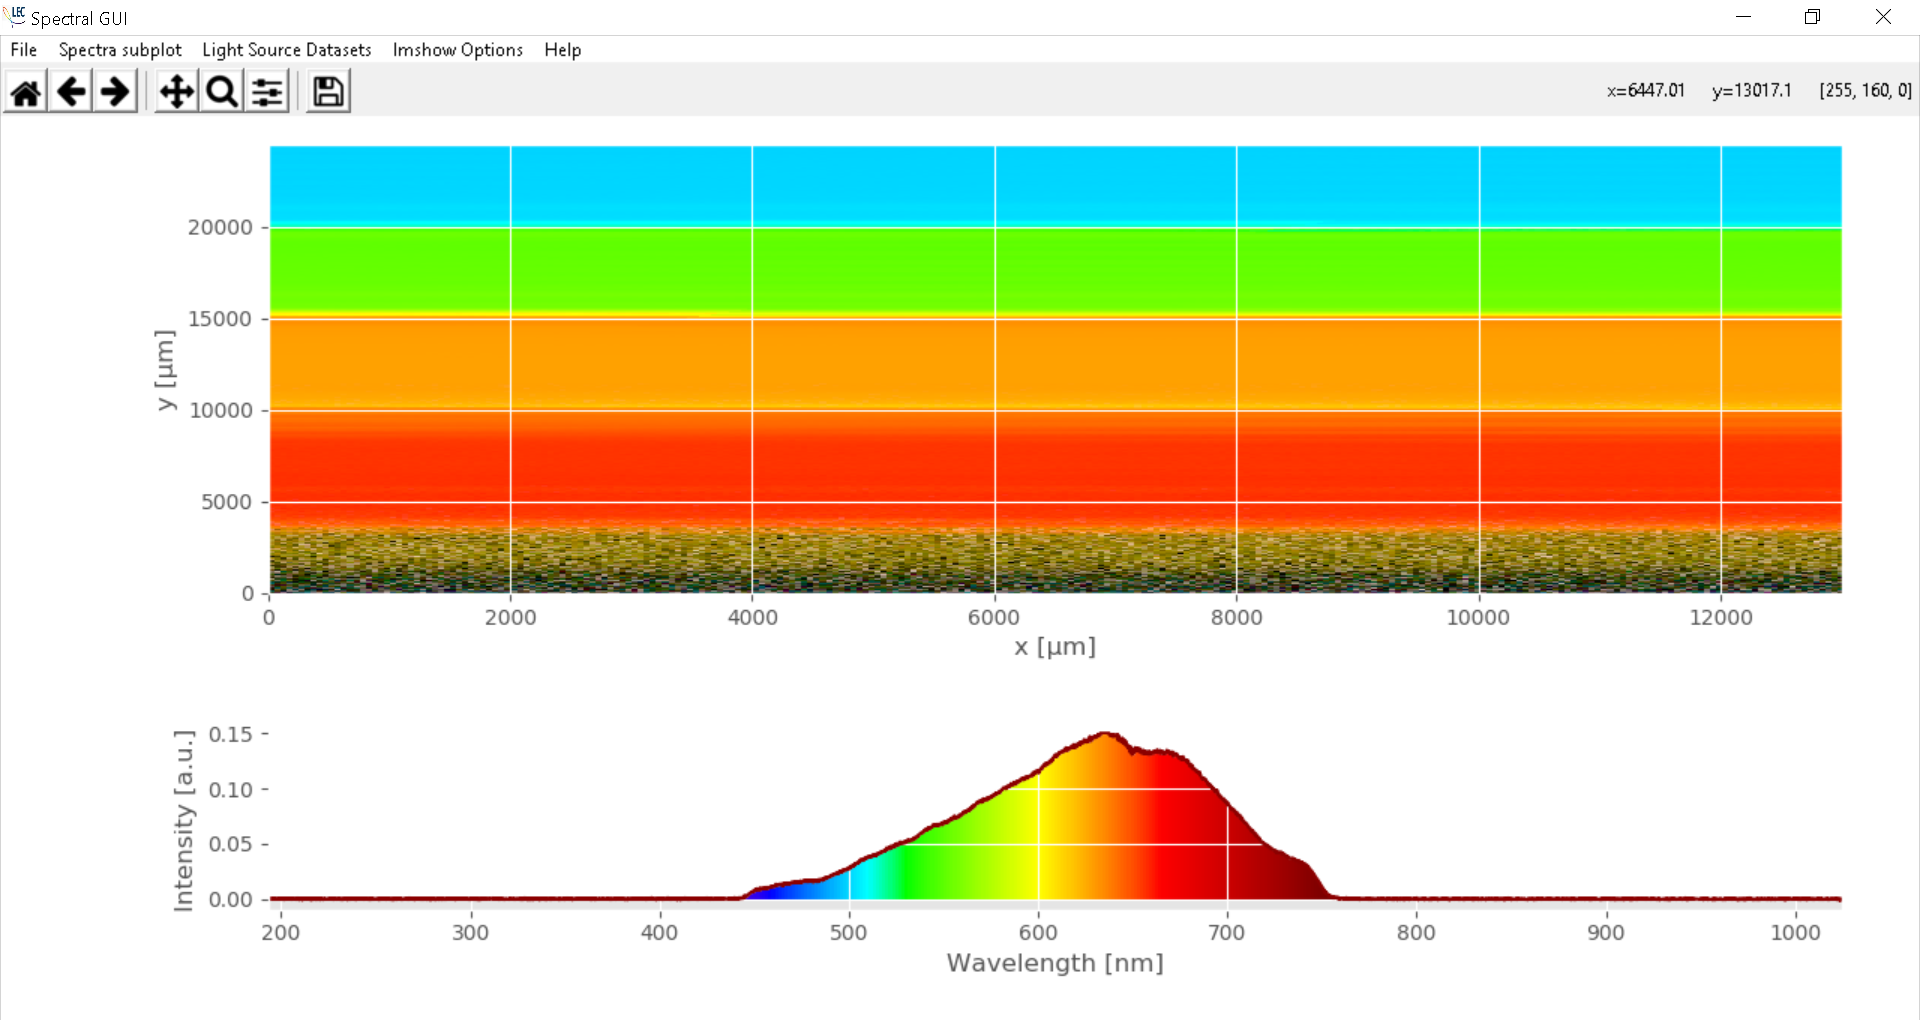
\includegraphics[width=1.0\textwidth]{Figs/microespectrometro/guirgb.png}
	\caption{Interfaz gráfica cuyo \textit{imshow} tenía una paleta de colores del espectro visible, de acuerdo al espacio de color CIE XYZ \cite{Wyman}.}
	\label{fig:GUI00}
\end{figure}


La interfaz gráfica fue realizada [\href{https://github.com/jrr1984/Prototipo0\_S-D\_SpectralGUI/blob/master/spectral\_gui/main.py}{\faGithub}] con la librería	 \href{https://wiki.python.org/moin/TkInter}{\textit{Tkinter}}. El barrido completo que se muestra en la imagen del mapa de colores de la Figura \ref{fig:GUI00} estuvo compuesto por 127920 mediciones de espectros de transmisión, que tomaron aproximadamente 18 horas de medición en total (Control remoto de la computadora con \href{https://anydesk.com/es}{AnyDesk} y control del experimento vía \href{https://pypi.org/project/cutelog/}{cutelog}, ver Sección \ref{sec:softadq}). Con la librería \href{https://pypi.org/project/colorpy/}{ColorPy} se obtuvo una tupla RGB a partir del espectro medido y cada tupla fue asignada a la posición medida del filtro. El conjunto total de todas las posiciones del filtro medidas estuvo formado por una matriz de 492 filas y 260 columnas. Dicha matriz fue mostrada como una imagen RGB con el método \textit{imshow} de la librería \textit{Matplotlib}. El gráfico debajo del \textit{imshow} muestra el espectro medido (gráfico de la intensidad detectada en función de la longitud de onda) para el píxel de la imagen sobre el cual se posicione el \textit{mouse} de forma actualizada y no muestra nada si se posiciona el mouse fuera de la imagen. 

En lugar de la imagen RGB de las mediciones también se puede mostrar el $\chi^{2}$ del espectro de transmisión de cada banda lo que permitiría ver la homogeneidad del espectro de transmisión de cada banda, que fue definido para la medición asociada a una posición (i,j) de cada banda de la siguiente manera:
\begin{equation}
\chi^{2}_{banda}(i,j) = \sum \frac{(medici\acute{o}n_{i,j} - espectro\_medio_{banda})^{2}}{medici\acute{o}n^{2}_{i,j}}
\end{equation}
donde $espectro\_medio_{banda}$ es el resultado de tomar el valor medio de todas las mediciones de una banda. En la Figura \ref{fig:GUI01} se muestra una región del filtro que contiene al cromo (en falso color amarillo) que separa la banda pancromática de la banda verde.
\begin{figure}[H]
	\centering
	\includegraphics[scale=0.41]{Figs/microespectrometro/chidisp.png}
	\caption{Interfaz gráfica con el \textit{imshow} del $\chi^{2}$ de cada banda. \textit{Zoom} sobre el cromo que separa la banda pancromática de la banda verde.}
	\label{fig:GUI01}
\end{figure}

La interfaz gráfica permite además graficar el espectro de un cierto píxel de la imagen generada a partir de la selección con el mouse, guardar imágenes de la región de interés, mostrar el espectro de la fuente de luz utilizada, etc, todas opciones que se consideraron útiles para la caracterización de las propiedades ópticas del filtro y deseadas para el prototipo final del equipo.

El prototipo preliminar permitió establecer las características deseadas del equipo final y evaluar su factibilidad sin incurrir en gastos importantes de prototipado. Ahora bien, debido a la falta de resolución óptica no se obtuvo ningún resultado concluyente ya que este prototipo resultó una prueba de concepto. A este prototipo se le propusieron las siguientes mejoras que fueron incluidas en el montaje y construcción del microespectrómetro [\ref{sec:montcontmsp}]:

\begin{enumerate}
\justifying
\item \texttt{Fuente de luz [\ref{sec:fteluzyesp}]}: Se modificó la fuente de luz de \textit{Fiber-Lite} que consiste de un \textit{fiber bundle} (arreglo de fibras ópticas) de un diámetro de 4.8 mm por una fuente de luz acoplada con una fibra óptica multimodo cuya apertura numérica fue de 0.22 y cuyo \textit{core} tenía un diámetro de 200 $\mu m$. Como no se contó con un objetivo adicional para enfocar la fuente de luz sobre el filtro y mediante un arreglo óptico elegir el tamaño del \textit{spot} incidente sobre el filtro , se decidió optar por la fuente de luz cuya salida divergente tuviera el menor ángulo del cono de luz de salida. Este criterio de diseño tenía como objetivo disminuir la región iluminada del filtro por la fuente de luz, lo que reduciría ciertas reflexiones espurias en los componentes ópticos del microespectrómetro provenientes de la luz de regiones no alcanzadas por el área de adquisición del microespectrómetro. Este efecto que aumenta proporcionalmente a la relación entre el área iluminada y el área adquirida del filtro se denomina efecto de Schwarzchild-Villiger \cite{Naora279} y debería ser considerado en las futuras mejoras del equipo aquí propuesto. Además la nueva fuente de luz utilizada tenía la misma fibra óptica que el espectrómetro, hecho que permitió realizar fácilmente la identificación de la región medida con el espectrómetro respecto de la imagen adquirida con la cámara \textit{web} (Ver Sección \ref{sec:camwebgui}).
\item \texttt{Platina [\ref{sec:platina}]}: Como la plataforma motorizada de Thorlabs utilizada en el prototipo preliminar tenía un límite de recorrido de 13 mm x 13 mm, no se podía adquirir el espectro de transmisión del filtro completo cuya región que contiene a las cinco bandas tiene unas dimensiones de 27 mm x 25 mm. En consecuencia se desarrolló una platina motorizada con el suficiente recorrido para poder realizar el barrido completo del filtro y también se consideró el paso y precisión mecánicas mínimas como para poder adquirir áreas de defectos de diámetro mayor a 20 $\mu m$ con la mayor cantidad de puntos posible, de forma tal de poder aprovechar el poder de resolución del microespectrómetro.
\item \texttt{Microespectrómetro [\ref{sec:montalin}]}: Se montó e incorporó al prototipo un microespectrómetro con una resolución óptica lateral diseñado para caracterizar defectos de diámetro mayor a 20 $\mu m$.
\item \texttt{Integración de una cámara \textit{web} [\ref{sec:camwebgui}]}: Se incorporó una cámara \textit{web} y un  \textit{joystick} al equipo para poder seleccionar la región del filtro a medir y se desarrolló una interfaz gráfica para poder visualizar en simultáneo la imagen digital de dicha región y el espectro de transmisión. 
\end{enumerate}

%%%%%%%%%%%%%%%%%%%%%%%%%%%%%%%%%%%%%%%%%%%%%%%%%%%%%%%%%%%%%%%%%%%%%%%%%%%%%%%%%%%%%%%%%%%%%%%%%%%%%%%%%%%%%%%%%%%%%%%%%%%%%%%%%%%%%%%%%%%%%%%%%%%%%%%%%%%%%%%%%%%%%%%%%%%%%%%%%%%%%%%%%%%%%%%%%%%%%%%%%%%%%%%%%%%%%%%%%%%%
\singlespacing
\section{Diseño y construcción del microespectrómetro}
\label{sec:montcontmsp}
\spacing{1.5}

\hspace{0.5cm}En esta sección se describen los criterios de diseño y todas las consideraciones técnicas del microespectrómetro, de la platina motorizada desarrollada que fue controlada con un \textit{joystick} y de la cámara \textit{web} integrada. En la Figura \ref{fig:presequipo} se muestra la última versión del equipo desarrollado. En las siguientes secciones se describen cada una de las partes del instrumento. El equipo final desarrollado de forma modular puede ser adaptado a requerimientos ópticos y mecánicos específicos distintos a los presentados en esta tesis.
\begin{figure}[H]
	\centering
	\includegraphics[scale=0.95]{Figs/microespectrometro/presentacion_equipo.png}
	\caption{Imagen de la última versión del equipo desarrollado.}
	\label{fig:presequipo}
\end{figure}



%%%%%%%%%%%%%%%%%%%%%%%%%%%%%%%%%%%%%%%%%%%%%%%%%%%%%%%%%%%%%%%%%%%%%%%%%%%%%%%%%%%%%%%%%%%%%%%%%%%%%%%%%%%%%%%%%%%%%%%%%%%%%%%%%%%%%%%%%%%%%%%%%%%%%%%%%%%%%%%%%%%%%%%%%%%%%%%%%%%%%%%%%%%%%%%%%%%%%%%%%%%%%%%%%%%%%%%%%%%%

\singlespacing
\subsection{Fuente de luz y espectrómetro \href{https://github.com/jrr1984/defects_analysis/blob/master/light_sources_spectrum.py}{\faGithub}}
\label{sec:fteluzyesp}
\spacing{1.5}

\hspace{0.5cm}El criterio de elección de la fuente de luz dependió fundamentalmente del rango de longitudes de onda que se quiso medir, que para el caso del filtro aquí analizado dicho rango se encontró entre los 450 nm y los 900 nm.
Se utilizó una fuente de luz halógena y de tungsteno modelo \href{https://www.thorlabs.com/newgrouppage9.cfm?objectgroup_id=7269&pn=SLS201L/M}{SLS201L} del fabricante Thorlabs (Ver Figura \ref{fig:fuentl}). 

\begin{figure}[H]
	\begin{floatrow}
		\ffigbox{\includegraphics[scale=0.5]{Figs/microespectrometro/sls201l.jpg}}{\caption{Imagen de la fuente de luz \href{https://www.thorlabs.com/newgrouppage9.cfm?objectgroup\_id=7269\&pn=SLS201L/M}{SLS201L} del fabricante Thorlabs.}\label{fig:fuentl}}
		\ffigbox{\includegraphics[scale=0.5]{Figs/microespectrometro/ccs200.jpg}}{\caption{Imagen del espectrómetro \href{https://www.thorlabs.com/thorproduct.cfm?partnumber=CCS200/M\#ad-image-0}{CCS200/M} del fabricante Thorlabs}\label{fig:ccs}}
	\end{floatrow}
\end{figure}

En la Figura \ref{fig:espfth} se muestra el espectro de emisión de la fuente de luz utilizada.  El espectrómetro utilizado para realizar las mediciones fue el \href{https://www.thorlabs.com/thorproduct.cfm?partnumber=CCS200/M#ad-image-0}{CCS200/M} del fabricante Thorlabs (Ver Figura \ref{fig:ccs}).

\begin{figure}[H]
	\centering
	\includegraphics[scale=0.5]{Figs/microespectrometro/espfuentethorl.png}
	\caption{Espectro de emisión de la fuente de luz \href{https://www.thorlabs.com/newgrouppage9.cfm?objectgroup\_id=7269&pn=SLS201L/M}{SLS201L} del fabricante Thorlabs [\href{https://github.com/jrr1984/defects\_analysis/blob/master/light\_sources\_spectrum.py}{\faGithub}].}
	\label{fig:espfth}
\end{figure}

El espectro de emisión de la fuente de luz reportado por el fabricante indica que debería ser en el rango de longitudes de onda de 360 - 2600 nm, lo cual se pudo verificar por lo menos en el rango comprendido entre los 200 nm y los 1000 nm que es el rango de detección del espectrómetro. El fabricante reportó una precisión del espectrómetro menor a los 2 nm y el tiempo de integración del detector de entre 10 $\mu s$ y 60 s.

%Además de considerar el espectro de emisión de la fuente de luz otro parámetro importante resultó la potencia de radiación de la misma ya que en función de ésta se eligen los tiempos de integración del espectrómetro para tener una buena relación señal-ruido. En consecuencia, una lámpara de mayor potencia reduce los tiempos de medición, lo que haría al método de inspección con el microespectrómetro más compatible con los tiempos de duración de los procesos industriales satelitales. La potencia de radiación de la lámpara reportada por el fabricante fue de 10mW.

 La fuente de luz \href{https://www.thorlabs.com/newgrouppage9.cfm?objectgroup_id=7269&pn=SLS201L/M}{SLS201L} (Ver Figura \ref{fig:fuentl}) del fabricante Thorlabs tiene una salida acoplada con una fibra óptica multimodo \href{https://www.thorlabs.com/newgrouppage9.cfm?objectgroup_id=6839&pn=FG200UCC}{FG200UCC} de una apertura numérica igual a 0.22 y cuyo \textit{core} tiene un diámetro de 200 $\mu m$. La fibra óptica de la fuente de luz es idéntica a la fibra óptica del espectrómetro. El conector SMA de la fibra óptica de color naranja que se muestra en la Figura \ref{fig:montttluz} fue conectado al adaptador \href{https://www.thorlabs.com/thorproduct.cfm?partnumber=SM1SMA\#ad-image-0}{SM1SMA} y éste a su vez fue montado sobre un \textit{cage} \href{https://www.thorlabs.com/thorproduct.cfm?partnumber=CP33}{CP33}. Al mismo tiempo dicho \textit{cage} fue montado con un vástago y una torreta a un posicionador micrométrico que permitió disminuir la distancia entre la fuente de luz y el filtro, de manera tal de poder reducir los tiempos de integración de la luz y en consecuencia reducir los tiempos de duración de cada barrido de una cierta región del filtro.
\begin{figure}[H]
	\centering
	\includegraphics[scale=0.15]{Figs/microespectrometro/setupactualdecote_retoc_condetalles.jpg}
	\caption{Montaje de la fuente de luz.}
	\label{fig:montttluz}
\end{figure}
 
%%%%%%%%%%%%%%%%%%%%%%%%%%%%%%%%%%%%%%%%%%%%%%%%%%%%%%%%%%%%%%%%%%%%%%%%%%%%%%%%%%%%%%%%%%%%%%%%%%%%%%%%%%%%%%%%%%%%%%%%%%%%%%%%%%%%%%%%%%%%%%%%%%%%%%%%%%%%%%%%%%%%%%%%%%%%%%%%%%%%%%%%%%%%%%%%%%%%%%%%%%%%%%%%%%%%%%%%%%%%

\singlespacing
\subsection{Platina \href{https://github.com/jrr1984/open\_frame\_XYStage}{\faGithub} \href{https://github.com/jrr1984/open_frame_XYStage/tree/master/3dprintedparts/STLs}{\faCubes}}
\label{sec:platina}
\spacing{1.5}

\hspace{0.5cm}Se desarrolló una platina de microscopía con dos grados de libertad para poder desplazar el filtro lateral y verticalmente respecto de la fuente de luz y del microespectrómetro para poder medir el espectro de transmisión del filtro en distintas regiones del mismo. Una imagen representativa de una de las primeras versiones de la platina con dos grados de libertad se muestra en la Figura \ref{fig:plato0}.


\begin{figure}[H]
	\centering
	\includegraphics[scale=0.16]{Figs/microespectrometro/stageearly.jpg}
	\caption{Imagen de una de las primeras versiones de la platina motorizada con dos grados de libertad.}
	\label{fig:plato0}
\end{figure}


La construcción y desarrollo de la platina motorizada del microespectrómetro consistió de las siguientes etapas de prototipado:

\begin{enumerate}
\item Investigación previa de la literatura sobre platinas de microscopía de bajo costo y factibles para integrar al prototipo.
\item Elección de los componentes y materiales en función de la oferta local en Argentina.
\item De acuerdo al ítem 2, se realizó un dimensionamiento de la platina y se determinó el recorrido total de cada uno de los grados de libertad. Esto permitió evaluar la factibilidad y aplicabilidad de la plataforma a desarrollar.
\item En conjunto con el diseñador industrial Federico Armesto se diseñaron las piezas de impresión 3D y se montó el primer eje de la platina. Se desarrolló la electrónica y el \textit{software} necesarios.
\item Una vez optimizado el diseño del primer eje, se montó el segundo eje de la platina. Se extendió el software y se integraron finales de carrera.
\item Desarrollo del \textit{software} de control de la platina. Calibración preliminar.
\item El prototipo de la platina seguía siendo actualizada al momento de escribir esta tesis.
\end{enumerate}

A continuación se describen algunas consideraciones técnicas y de diseño que se tuvieron en cuenta para el desarrollo de la platina motorizada y que podrían ser de utilidad para otros laboratorios que quisieran replicar la plataforma que aquí se presenta, realizar una adaptación ó simplemente como fuente de consulta.

Respecto de la revisión de la literatura sobre platinas de microscopía de bajo costo y factibles para el prototipo, se consultaron  los prototipos cuyos proyectos hayan sido desarrollados bajo la modalidad \textit{open source} tanto para la distribución del diseño de las piezas 3D como del \textit{software}, dentro de las cuales se destacan \cite{schaa}(\textit{LabView}, EUR 250) y \cite{campbells}(Instrucciones vía puerto serie en \textit{Matlab}, \textit{LabView} y \textit{python}, USD 1000). Dichas propuestas son también denominadas en cierto contexto DIY (\textit{Do it yourself}) ya que contienen toda la documentación y herramientas necesarias para que cualquier usuario con presupuesto y acceso a los mismos componentes pueda reproducir el proyecto. Además de estos proyectos se consultaron múltiples platinas de microscopía comerciales, donde en sus páginas \textit{web} la mayoría de los fabricantes distribuyen los planos de diseño, las piezas 3D libres para modificar, etc (\href{https://www.thorlabs.com/newgrouppage9.cfm?objectgroup\_id=2132}{NRT150 Thorlabs} USD 2456 x 2, \href{https://www.edmundoptics.com/p/150mm-motorized-stage/16419/}{\#59-747 EO} USD 2095 x 2). Ahora bien, hasta la fecha de escritura de este trabajo no se registraban prototipos de platinas motorizadas de microscopía desarrolladas en laboratorios del país como la que aquí se presenta por lo cual por medio de la presente se comparten las piezas de diseño 3D y el \textit{software} necesarios para poder replicarla y extender sus prestaciones. El costo total aproximado de la platina aquí desarrollada fue de USD 200 (Ver Facturas: \href{https://github.com/jrr1984/open\_frame\_XYStage/tree/master/Facturas\_costos}{\faMoneyCheck}).

El tipo de platina motorizada a desarrollar dependió del presupuesto, de la oferta local de los componentes y de los requerimientos mecánicos de precisión, longitud de recorrido y repetibilidad. Estos tres conceptos se encontraban relacionados fuertemente entre sí. Si bien se podrian haber comprado los componentes de la platina en el exterior del país, la futura necesidad de comprar nuevamente alguno de los componentes debido al desgaste ó rotura de los mismos, hacen de esta implementación de la compra una mala práctica del prototipado. En este sentido se eligieron componentes masivos en el país, los cuales se podían conseguir fácilmente sus repuestos en caso de necesidad. Al mismo tiempo, los componentes masivos son los que tienen un menor costo debido a su mayor demanda.

A modo de referencia pero no de publicidad se consultaron fundamentalmente tres proveedores de componentes mecánicos y de electrónica, de la ciudad de Buenos Aires y de la provincia de Buenos Aires: \href{https://3dinsumos.com.ar/}{3DInsumos} (Caseros, Buenos Aires), \href{https://ingia.com.ar/}{Ingia Automatización}(Saavedra, C.A.B.A.) y \href{https://candy-ho.com/}{Candy-Ho} (Villa Martelli, C.A.B.A.). A partir de la oferta de estos y otros proveedores se eligieron los componentes de la platina tomando como idea de diseño e implementación la platina de \cite{schaa} que por su bajo costo y la utilización de piezas 3D que facilitaban el prototipado rápido (dependiendo de la disponibilidad de una impresora 3D), hacían de esa propuesta la más indicada para ser implementada.

Los componentes principales de la platina son el motor paso a paso y el sistema de transmisión que transforma la rotación del motor en un desplazamiento lineal. Uno de los motores paso a paso más populares del mercado sino el más popular es el \href{https://www.pololu.com/product/1200}{NEMA 17} que es ampliamente utilizado en impresoras 3D y CNC. Por este motivo se eligió ese motor en lugar del \href{https://www.pololu.com/product/1204}{NEMA 8} utilizado en \cite{schaa}, que sólo se podía conseguir haciendo un pedido al exterior lo que encarece su costo y alarga notablemente los tiempos de prototipado.

De la familia de motores paso a paso NEMA 17 (Ver Figura \ref{fig:nema17}) existen distintos modelos dependiendo los requerimientos de torque y de resolución fundamentalmente. El torque no fue una limitante para la elección del modelo con lo cual en función de las distintas opciones de torque se priorizó el de menor precio. Ahora bien, respecto de la precisión existen dos modelos con pasos mínimos de rotación de 1.8 grados y de 0.9 grados, con lo cual se tienen 200 y 400 pasos por revolución respectivamente. Se evaluó la oferta disponible en el mercado y se eligieron motores NEMA 17 con un paso mínimo de 0.9 grados con el fin de obtener la mayor resolución en el desplazamiento lineal, a pesar de que su costo era mayor.

A la elección del motor, le sigue la elección del sistema de transmisión donde existen múltiples opciones dependiendo de la precisión, entre ellas las correa dentadas con poleas, las varillas roscadas, los husillos de bolas, etc. De acuerdo a \cite{schaa} se optó por una varilla roscada masiva en el mercado del tipo \href{https://www.mcmaster.com/acme-screws/acme-lead-screws-and-nuts/}{ACME} (Ver Figura \ref{fig:acmea}) de un diámetro de 8 mm y con un paso (\textit{pitch}) de 2 mm, es decir que por cada revolución completa del motor se realiza un desplazamiento lineal de 2 mm. La rotación del motor paso a paso es transferida a la varilla roscada ACME por medio de un acople sólido con agujeros para prisioneros M3 equidistanciados a 180° para que la varilla roscada quede centrada, que fue diseñado (Ver \href{https://github.com/jrr1984/open_frame_XYStage/blob/master/3dprintedparts/STLs/acopleRIGIDO.STL}{\faCubes}).
\begin{figure}[H]
	\begin{floatrow}
		\ffigbox{\includegraphics[scale=0.7]{Figs/microespectrometro/nema17.jpg}}{\caption{Motor paso a paso \href{https://www.pololu.com/product/1200}{NEMA 17} con una resolución de 400 pasos por revolución (0.9° por paso).}\label{fig:nema17}}
		\ffigbox{\includegraphics[scale=0.7]{Figs/microespectrometro/acmeantib.jpg}}{ \caption{Varilla roscada del tipo \href{https://www.mcmaster.com/acme-screws/acme-lead-screws-and-nuts/}{ACME} con un paso (\textit{pitch}) de 2 mm  y un diámetro de 8 mm, junto con una tuerca \textit{anti-backslash}}\label{fig:acmea}}
	\end{floatrow}
\end{figure}

Además del sistema de transmisión se tuvo que elegir un sistema de desplazamiento que es el que permite el movimiento de los ejes de la platina. Se eligió la opción más utilizada en impresoras 3D en el que se utilizan sistemas lineales con barras rectificadas de acero de 6mm de diámetro y rodamientos lineales \href{https://uk.misumi-ec.com/vona2/detail/221000091678/?HissuCode=LM6LUU}{LM6LUU}. Dichos rodamientos y la tuerca \textit{antibackslash} fueron montados sobre un cubo diseñado e impreso con una impresora 3D (Ver \href{https://github.com/jrr1984/open_frame_XYStage/blob/master/3dprintedparts/STLs/cuboconLM6UU_2demarzo.STL}{\faCubes}) que realizó los desplazamientos lineales al deslizarse sobre las barras de acero.

La resolución espacial mecánica es el mínimo desplazamiento de cada uno de los ejes de la platina. La misma viene dada teóricamente por la siguiente ecuación:
\begin{equation}
\text{Resolución} [\mu m / paso] = \frac{\text{\textit{Pitch} del ACME}}{\text{\# de pasos por revolución del motor}} = \frac{2 mm}{400 pasos} = \frac{5 \mu m}{paso}
\end{equation}

Además esta resolución fue modificada por medio de la electrónica que controla los motores paso a paso implementando una técnica que se conoce como \textit{microstepping} \cite{7806244}. Esta técnica permite al motor realizar rotaciones de ángulos menores al paso mínimo del motor, con lo cual se mejora la resolución ya que se puede subdividir un paso completo del motor en 2,4,8,16 e incluso hasta en 32 pasos (teóricos). Al mismo tiempo se reduce el ruido del motor y el movimiento del mismo se suaviza. La técnica es impelementada por el controlador de corriente que utiliza un algoritmo que a su salida envía una modulación sinusoidal discretizada de la corriente, donde cada paso de dicha modulación sinusoidal consiste de un micropaso y el período de la señal es igual al paso completo original del motor.

Los dos controladores de corriente de los motores paso a paso más populares con la capacidad de aplicar \textit{microstepping} son el \href{https://www.pololu.com/product/2133}{DRV8825}(hasta 32 micropasos y 2.5 A) y el \href{https://www.pololu.com/product/1182}{A4988} (hasta 16 micropasos y 2 A). Se eligió finalmente para la platina el \textit{driver} A4988 (Ver Figura \ref{fig:a4988}) y se limitó la máxima corriente que podía entregar de acuerdo al consumo observado de los motores en condiciones de operación normales, ajustando el potenciómetro (Ver Figura \ref{fig:a4988}) a partir de la medición de una tensión de referencia de acuerdo a las especificaciones del manual del fabricante \cite{a4988}.

\begin{figure}[H]
    \begin{floatrow}
        \ffigbox{\includegraphics[scale=0.3]{Figs/microespectrometro/a4988.jpg}}{\caption{Controlador de los motores paso a paso A4988.}\label{fig:a4988}}
        \ffigbox{\includegraphics[scale=0.8]{Figs/microespectrometro/megaramps.jpg}}{ \caption{\href{https://store.arduino.cc/usa/mega-2560-r3}{\textit{Arduino MEGA 2560}} a la derecha en azul y \href{https://reprap.org/wiki/RAMPS_1.4}{\textit{Shield RAMPS 1.4}} a la izquierda en rojo. }\label{fig:ramps}}
    \end{floatrow}
\end{figure}

Se utilizó un \href{https://store.arduino.cc/usa/mega-2560-r3}{\textit{Arduino MEGA 2560}} para controlar la lógica de la platina vía el puerto USB de una computadora y se le montó a los pines hembra del arduino un \textit{shield} \href{https://reprap.org/wiki/RAMPS_1.4}{\textit{RAMPS 1.4}} donde se colocaron los \textit{drivers} de los motores, las conexiones de los finales de carrera y el \textit{joystick}. La RAMPS fue alimentada de forma independiente con una fuente de tensión.

Antes de realizar la compra de los componentes necesarios para montar el primer eje se determinó el recorrido total de cada uno de los grados de libertad de la platina de acuerdo a la oferta de los proveedores. Por ejemplo, existen comercialmente distintas longitudes de varillas roscadas ACME y se eligió una longitud de la misma de 500 mm, de forma tal que al cortar dicha varilla se pueda obtener las dos varillas necesarias para cada eje de la platina, cada una de 250 mm de largo. El mismo razonamiento fue aplicado a las varillas de acero de 6 mm de diámetro, para las cuales se compraron dos varillas de 1 metro que cada una fue cortada en cuatro partes de 250 mm cada una. De esta manera, se realizó un diagrama con las dimensiones y la longitud de recorrido estimada de uno de los ejes de la platina con el software \textit{Solidworks} como se muestra en la Figura \ref{fig:dimejee}.

\begin{figure}[H]
	\centering
	\includegraphics[scale=0.9]{Figs/microespectrometro/dimensio.png}
	\caption{Estimación del recorrido de uno de los ejes de la platina.}
	\label{fig:dimejee}
\end{figure}

El objetivo de esta etapa del prototipado fue el de evaluar la factibilidad y aplicabilidad de la platina para poder desplazar al filtro respecto de la fuente de luz y del espectrómetro de manera tal de poder obtener una medición del espectro en cualquier región del filtro deseada. Luego de realizar el dimensionamiento, se decidió montar el eje $\textit{x}$ de la platina únicamente. En la Figura \ref{fig:dise1eje} se muestra el diseño del eje $\textit{x}$ realizado con el software libre \textit{Fusion 360} y en la Figura \ref{fig:1ejmontado} se muestra un montaje preliminar de dicho eje\footnote{Se imprimió inicialmente una porción del cubo diseñado como prueba preliminar, ya que la impresión del cubo completa podía tomar más de 10 horas. Resultó importante realizar pruebas por etapas para reducir los tiempos de prototipado.}. 

\begin{figure}[H]
	\begin{floatrow}
		\ffigbox{\includegraphics[scale=0.83]{Figs/microespectrometro/diseo1eje.png}}{\caption{Diseño de las piezas 3D del eje $\textit{x}$ de la platina [\href{https://github.com/jrr1984/open_frame_XYStage/blob/master/3dprintedparts/STLs/Ejexpreliminar.stl}{\faCubes}].}\label{fig:dise1eje}}
		\ffigbox{\includegraphics[scale=0.073]{Figs/microespectrometro/1ejemontado.jpg}}{\caption{Montaje preliminar del eje $\textit{x}$ de la platina.}\label{fig:1ejmontado}}
	\end{floatrow}
\end{figure}


Luego de optimizar el diseño y montaje del primer eje, se montó el eje $\textit{y}$ compuesto por las mismas piezas 3D que el eje $\textit{x}$. En este sentido se hace notar que el diseño propuesto resultó una solución completamente modular y que la configuración de los ejes aquí adoptada puede ser modificada a otras de acuerdo a las necesidades del usuario final. 
 
\begin{figure}[H]
	\begin{floatrow}
		\ffigbox{\includegraphics[scale=0.83]{Figs/microespectrometro/scanningstage.jpg}}{\caption{Diseño preliminar de los dos ejes de la platina.}\label{fig:dise1eje}}
		\ffigbox{\includegraphics[scale=0.13]{Figs/microespectrometro/2ejesmontaje.jpeg}}{\caption{Montaje final de la de la platina.}\label{fig:1ejmontado}}
	\end{floatrow}
\end{figure}

%%%%%%%%%%%%%%%%%%%%%%%%%%%%%%%%%%%%%%%%%%%%%%%%%%%%%%%%%%%%%%%%%%%%%%%%%%%%%%%%%%%%%%%%%%%%%%%%%%%%%%%%%%%%%%
%%%%%%%%%%%%%%%%%%%%%%%%%%%%%%%%%%%%%%%%%%%%%%%%%%%%%%%%%%%%%%%%%%%%%%%%%%%%%%%%%%%%%%%%%%%%%%%%%%%%%%%%%%%%%%

\singlespacing
\subsubsection{\textit{Software} de control de la platina \href{https://github.com/jrr1984/open\_frame\_XYStage}{\faGithub}  y calibración preliminar}
\label{sec:softcalib}
\spacing{1.5}

\hspace{0.5cm}Se desarrolló un \textit{software} de control de la platina que fue integrado al \textit{software} de control del espectrómetro y de la cámara \textit{web}. En [\cite{campbells},\href{https://github.com/raacampbell/openstage/tree/master/serialInterfaceScripts}{\faGithub}] se desarrollaron instrucciones específicas de comandos a ejecutar vía el puerto serie al que se conectó el arduino que controla la lógica de la platina, por medio de los lenguajes de programación \textit{Matlab}, \textit{LabView} y \textit{python}. En el proyecto \textit{open source} \href{https://www.youtube.com/watch?v=Lm8oprDhAnQ}{RDL} [\href{https://forum.arduino.cc/index.php?topic=469343}{\faCode}] se desarrolló un \textit{software} de comandos muy exhaustivo a ejecutar únicamente por el puerto serie de arduino.

El \textit{software} de control de la platina fue organizado como se muestra en la Figura \ref{fig:cnpl}. A nivel del microcontrolador las instrucciones a los \textit{drivers} que regulan la corriente de los motores y le envían los pulsos PWM para que realicen la cantidad de pasos elegidos fueron desarrolladas con la librería de \textit{Arduino} \href{https://www.airspayce.com/mikem/arduino/AccelStepper/}{AccelStepper}. Dichas instrucciones escritas en el lenguaje de programación propio de arduino incluyen métodos para asignarle las posiciones de los motores, para leer las posiciones de los motores, para prenderlos, apagarlos, determinar si llegaron a la posición asignada ó no, para ponerlos en la posición inicial de la platina, para leer los finales de carrera, etc. Todos los métodos escritos se pueden ver en el \textit{header} del \textit{driver} desarrollado [\href{https://github.com/jrr1984/open_frame_XYStage/tree/master/ino_main}{\faGithub}].
Ahora bien, para poder integrar el control de la platina con el espectrómetro y con la cámara se tuvo que establecer una comunicación por medio de mensajes a través del puerto serie de la computadora. Para ello se utilizó la librería \href{https://github.com/kroimon/Arduino-SerialCommand}{\textit{SerialCommand}} que permitió unir la lógica a nivel del microcontrolador del \textit{Arduino} con la lógica a nivel del procesador de la computadora. De esta manera, en el lenguaje de programación \textit{python} se escribió una clase [\href{https://github.com/jrr1984/open\_frame\_XYStage/blob/master/XYStage.py}{\faGithub}] con los mismos métodos de control de la platina escritos con la librería \textit{AccelStepper} en \textit{Arduino} de forma tal de enviar mensajes al puerto serie de la computadora que el \textit{Arduino} se encontraba constantemente escuchando. Así por ejemplo, desde \textit{python} se envía un mensaje al puerto serie para mover el motor del eje $\textit{x}$ una distancia de 2 mm, el \textit{Arduino} escucha ese mensaje y le envía los pulsos PWM al motor para realizar el desplazamiento. En la Sección \ref{sec:softadq} se explica el \textit{software} desarrollado para automatizar las mediciones que integró el control de la platina con el espectrómetro y la cámara.

\begin{figure}[H]
	\centering
	\includegraphics[scale=0.5]{Figs/microespectrometro/diagflujoplatina.png}
	\caption{Diagrama de la comunicación vía el puerto serie de la computadora entre el microcontrolador \textit{Arduino} y el proceso principal de la computadora programado en \textit{python} en el que se integró el espectrómetro y la cámara.}
	\label{fig:cnpl}
\end{figure}

Se realizó una calibración preliminar de la platina para determinar las incertezas de su resolución (mínimo paso de desplazamiento) que fueron luego utilizadas en la medición de la resolución espacial del microespectrómetro (Ver Sección \ref{sec:focoresol}). En el trabajo de \cite{schaa} realizaron una calibración de la platina adquiriendo sucesivas imágenes de una muestra calibrada de distancias (1951 USAF \textit{test target}), midiendo el desplazamiento relativo respecto de un punto de referencia situado en la imagen inicial adquirida. Al momento de escribir esta tesis se iba a realizar la calibración con el mismo método. El \textit{software} de adquisición ya se había desarrollado [\href{https://github.com/jrr1984/defectsGUI/blob/master/views.py}{\faGithub}] y ya se contaba con una pieza 3D impresa que hacía de soporte de una regla calibrada de microscopía colocada sobre un portamuestra, para realizar la calibración de la platina.

Ahora bien, en primer lugar se midió la precisión y exactitud de los desplazamientos de la platina en el orden de los milímetros. Para ello, por medio del \textit{software} desarrollado se asignaron posiciones a cada uno de los ejes de la platina y se comparó el valor medido con una regla metálica calibrada en milímetros con los valores asignados por \textit{software}. Se observó que la platina tenía exactitud en milímetros, ya que no se encontraron diferencias entre los valores de las posiciones asignadas y las posiciones medidas. Y, de la repetición de las mediciones se verificó su precisión en milímetros ya que las mediciones no presentaron dispersiones en los valores obtenidos.

Para medir la precisión y exactitud en el orden de los micrones, se utilizaron las mediciones del microespectrómetro como calibración preliminar. Se eligió la resolución teórica de 1 $\mu m$ del desplazamiento de cada eje de la platina en la adquisición de barridos de ciertas regiones del filtro con el microespectrómero. Dicha resolución representa el desplazamiento mínimo que cada eje de la platina podría realizar y su valor fue elegido considerando un compromiso entre el tiempo de duración de un barrido y la resolución del mismo ya que en cada paso de la platina se realiza una medición individual.
En primer lugar se utilizó como patrón de calibración la longitud del cromo que separa dos bandas del filtro medida con el microscopio Zeiss (Ver Sección \ref{subs:compl}). En la Figura \ref{fig:barrcromoo} se muestra el barrido del cromo entre las bandas roja y pancromática realizado con un paso de 1 $\mu m$.

\begin{figure}[H]
	\centering
	\includegraphics[width=1.0\columnwidth]{Figs/microespectrometro/barridocromocalib.png}
	\caption{Gráfico de la intensidad total detectada en función de la posición medida del filtro en un barrido lineal del cromo que separa las bandas roja de la pancromática.}
	\label{fig:barrcromoo}
\end{figure}

En el gráfico de la Figura \ref{fig:barrcromoo} se muestra la intensidad total detectada, esto es la suma de la intensidad detectada para cada longitud de onda del espectro medido, en función de la posición del filtro. El barrido fue lineal, es decir en una dimensión. Se asignó por \textit{software} a la platina un desplazamiento de 1000 $\mu m$, con un paso de 1 $\mu m$. En cada paso de la platina el microespectrómetro obtuvo una medición del espectro. Los espectros no fueron normalizados con la fuente de luz y es por eso que se puede observar un mayor valor de intensidad total para la banda pancromática que para la banda roja. El valor del cromo que separa la banda roja de la pancromática medido con el \textit{software} Fiji de una imagen completa del filtro adquirida con el microscopio Zeiss fue de $( 516 \pm 10) \mu m$.
Para determinar el valor medido de la longitud del cromo con el microespectrómetro se ajustó cada transición de una banda al cromo con la función error, \textit{erf(x)}, que es la integral del perfil gaussiano del haz de luz en una dimensión. La función utilizada para el ajuste fue:
\begin{equation}
\frac{a}{2}\hspace{2pt}.\hspace{2pt}erf\left(\sqrt{2}\hspace{1pt}.\hspace{1pt}\frac{(x-b)}{c}\right)
\label{eq:iz}
\end{equation}
\begin{equation}
\frac{a}{2}\hspace{2pt}.\hspace{2pt}\left(1+erf\left(\sqrt{2}\hspace{1pt}.\hspace{1pt}\frac{(x-b)}{c}\right)\right),
\label{eq:der}
 \end{equation} para la transición izquierda [\ref{eq:iz}] y derecha [\ref{eq:der}] respectivamente. Así por ejemplo para el barrido de la Figura \ref{fig:barrcromoo} se ajustaron ambas transiciones como se muestra en las Figuras \ref{fig:ajusteladoizq} y \ref{fig:ajusteladoder}. En azul se muestra el resultado del ajuste y los puntos rojos fueron datos eliminados de cada ajuste.
\begin{figure}[H]
	\begin{floatrow}
		\ffigbox{\includegraphics[scale=0.17]{Figs/microespectrometro/ajustebarrladoizq.png}}{\caption{Ajuste de los datos de la transición de la banda roja al cromo por una función \textit{erf(x)}.}\label{fig:ajusteladoizq}}
		\ffigbox{\includegraphics[scale=0.17]{Figs/microespectrometro/ajustebarrladoder.png}}{\caption{Ajuste de los datos de la transición del cromo a la banda pancromática por una función \textit{erf(x)}.}\label{fig:ajusteladoder}}
	\end{floatrow}
\end{figure}

A partir de los parámetros del ajuste se determinó la longitud medida del cromo, $l_{cromo}$ de la siguiente manera:
\begin{equation}
l_{cromo} = (b_{der} - c_{der}) - (b_{izq} + c_{izq}),
\end{equation}
donde $b_{izq}, c_{izq}, b_{der} yc_{der}$ son los parámetros del ajuste de la transición entre la banda roja y el cromo (izq) y entre el cromo y la banda pancromática (der). Así, para el barrido que se muestra en la Figura \ref{fig:barrcromoo} se obtuvo una longitud del cromo igual a 540 micrones, con lo cual para esta medición la diferencia entre el valor medido con el microespectrómetro y el valor tomado como referencia medido con el Zeiss, fue del 5\%.

En esta sección se describió la platina desarrollada para poder caracterizar al filtro en cualquier punto del mismo y con la suficiente resolución como para poder muestrear correctamente la resolución óptica del microespectrómetro, que se explica en la Sección \ref{sec:caractequipo}. A continuación se muestra un resumen de las características principales de la platina desarrollada y las futuras mejoras que serán implementadas además la calibración y caracterización que quedaron pendientes.

\newpage
\begin{figure}[H]
\begin{minipage}{0.47\textwidth}
\centering
\includegraphics[width=.7\textwidth,left]{Figs/microespectrometro/descarga.png}
\end{minipage}
\hfill
\begin{minipage}{0.47\textwidth}
\raggedleft
\Huge \textbf{XY(Z) Open Frame Stage}
\end{minipage}
\end{figure}

\texttt{Características principales y futuras mejoras:}

    \begin{itemize}
        \item Grados de libertad: 2. Ejes $\textit{x}$ e $\textit{y}$  .
        \item Longitud de recorrido de cada grado de libertad $>$ 240 mm.
        \item Motores paso a paso NEMA 17, 0.9° de paso mínimo, 400 pasos por revolución, $I_{máx} = 1.67 A$, $V = 4V$.
        \item Transmisión vía varilla ACME, paso 2 mm, diámetro 8 mm. Tuerca \textit{antibackslash}.
        \item \textit{Drivers} de corriente disponibles y \textit{microstepping}:
\begin{itemize}
\item A4988, hasta 2 A. Opciones de \textit{microstepping:} 1, 2, 4, 8 y 16. $\xrightarrow{}$ Resoluciones (teóricas) de 5 $\mu m$, 2.5 $\mu m$, 1.25 $\mu m$ y 0.63 $\mu m$ respectivamente.
\item DRV8825, hasta 2.5 A. Opciones de \textit{microstepping:} 1, 2, 4, 8, 16 y 32. $\xrightarrow{}$ Resoluciones (teóricas) de 5 $\mu m$, 2.5 $\mu m$, 1.25 $\mu m$, 0.63 $\mu m$ y 0.31 $\mu m$ respectivamente. 
\end{itemize}
\item Finales de carrera.
\item \textit{Joystick} para manipular la platina manualmente.
    \item Mejoras (actualidad):
    \begin{itemize}
 	\item Calibración de la platina con la cámara integrada al microespectrómetro [\cite{schaa}].
 	\item Caracterización de la precisión y de la repetibilidad de la platina.
        \item Implementación de rodamientos lineales LM6LUU en el eje $\textit{y}$.
        \item Integración y desarrollo de un tercer grado de libertad, del eje $\textit{z}$, que permita variar la distancia entre el objetivo y el filtro de forma automatizada.
        \item Inclusión de finales de carrera en el eje $\textit{y}$ y en el eje $\textit{z}$. 
        \end{itemize}
\end{itemize}
\newpage


%%%%%%%%%%%%%%%%%%%%%%%%%%%%%%%%%%%%%%%%%%%%%%%%%%%%%%%%%%%%%%%%%%%%%%%%%%%%%%%%%%%%%%%%%%%%%%%%%%%%%%%%%%%%%%%%%%%%%%%%%%%%%%%%%%%%%%%%%%%%%%%%%%%%%%%%%%%%%%%%%%%%%%%%%%%%%%%%%%%%%%%%%%%%%%%%%%%%%%%%%%%%%%%%%%%%%%%%%%%%

\singlespacing
\subsection{Diseño óptico, montaje y alineación del microespectrómetro}
\label{sec:montalin}
\spacing{1.5}

\hspace{0.5cm}En la Figura \ref{fig:micromfinal} se muestra el montaje y los componentes de la versión actual del microespectrómetro. 
\begin{figure}[H]
	\centering
	\includegraphics[width=1.0\textwidth]{Figs/microespectrometro/microespectrometroo_actual.png}
	\caption{Componentes ópticos y montaje del microespectrómetro.}
	\label{fig:micromfinal}
\end{figure}
El diagrama del camino óptico del microespectrómetro se muestra en la Figura \ref{fig:diagcaminoopt}\footnote{Los diagramas ópticos fueron realizados con el \textit{software} libre \href{https://inkscape.org/es/}{Inkscape}, utilizando una librería de componentes [\href{http://www.gwoptics.org/ComponentLibrary/}{Alexander Franzen lib.]}}. La luz que sale divergente de la fibra óptica (Ver Figura \ref{fig:montttluz}) incide perpendicularmente sobre el filtro. La luz transmitida por el filtro es recolectada por un objetivo de microscopio \href{https://www.edmundoptics.com/p/10x-mitutoyo-plan-apo-infinity-corrected-long-wd-objective/6623/}{Mitutoyo} corregido al infinito, de distancia de trabajo larga (34 mm), magnificación 10X y una apertura numérica igual a 0.28. La luz que sale corregida al infinito del objetivo es enfocada con una lente biconvexa de distancia focal igual a 200 mm de forma simultánea a la fibra del espectrómetro y a un sensor CMOS de una cámara \textit{web} \href{https://www.microsoft.com/accessories/es-xl/d/lifecam-hd-3000}{Lifecam HD 3000}, por medio de un \textit{beamsplitter} 10:90 (R:T) \href{https://www.thorlabs.com/thorproduct.cfm?partnumber=BSN10R}{BSN10R}. El \textit{beamsplitter} refleja un 10\% de la luz a la cámara y transmite el 90\% a la fibra óptica acoplada al espectrómetro. 
\begin{figure}[H]
	\centering
	\includegraphics[width=1.0\textwidth]{Figs/microespectrometro/diagopticosetup.png}
	\caption{Diagrama del camino óptico del microespectrómetro.}
	\label{fig:diagcaminoopt}
\end{figure}

El objetivo fue montado sobre un componente optomecánico \href{https://www.thorlabs.com/thorProduct.cfm?partNumber=SM1Z\#ad-image-0}{SM1Z} de Thorlabs que permitió modificar la distancia entre el objetivo y el filtro para poner en foco al microespectrómetro (Ver Sección \ref{sec:focoresol}). El SM1Z tiene una longitud de recorrido de 2 mm, paso de 1 $\mu m$ y por cada revolución se tiene un desplazamiento lineal de 50 $\mu m$.  La lente de tubo (en inglés, \textit{tube lens}) fue montada sobre un \href{https://www.thorlabs.com/thorproduct.cfm?partnumber=SM1V15}{SM1V15} que permitió modificar la distancia entre la lente de tubo y la fibra del espectrómetro para su alineación. El SM1V15 fue montado sobre un \textit{cage} CP33. El beamsplitter de forma rectangular fue sujetado por un adaptador \href{https://www.thorlabs.com/thorproduct.cfm?partnumber=FFM1\#ad-image-0}{FFM1} y éste fue asegurado con dos tornillos sobre la tapa del cubo \href{https://www.thorlabs.com/thorproduct.cfm?partnumber=C6W}{C6W}. La fibra óptica del espectrómetro se conectó al \textit{cage} \href{https://www.thorlabs.com/thorproduct.cfm?partnumber=CXY1\#ad-image-0}{CXY1} que tiene una longitud de recorrido en \textit{x} e \textit{y} de 1 mm para ajustar su posición. La cámara \textit{web} fue colocada sobre un \textit{cage} impreso en una impresora 3D [\href{https://github.com/jrr1984/open_frame_XYStage/blob/master/3dprintedparts/STLs/CAGE\_1pulgada.STL}{\faCubes}]. Todo el sistema fue montado con barras de 6 mm de diámetro de Thorlabs.

Otros montajes de microespectrómetros consultados en la literatura pero distintos al presentado aquí se pueden ver en \cite{frosch}, \cite{wong}, \cite{mour}(por reflexión) y \cite{frise} (adaptación de bajo costo de un microscopio comercial). Además, se consultaron soluciones comerciales como las de los fabricantes \href{https://andor.oxinst.com/learning/view/article/modular-solutions-for-microspectroscopy}{Andor} y \href{http://www.microspectra.com/}{CRAIC}.

Para alinear la fuente de luz con el objetivo, se retiró el filtro del medio del sistema de iluminación y de detección con la platina (subiéndolo hacia arriba, no hizo falta desmontarlo) y se alineó el \textit{cage} de la fibra óptica de la fuente de luz con el SM1Z del objetivo. De esta manera se alineó el plano perpendicular al eje óptico (eje $\textit{z}$) contenido por los ejes $\textit{x} e \textit{y}$ (ver Figura \ref{fig:plato0}) entre la fuente de luz y el microespectrómetro. Esta alineación fue realizada para maximizar la intensidad de la luz detectada.

La alineación de la lente de tubo y del objetivo fueron realizadas de forma previa al montaje final del equipo. Para alinear la lente de tubo (Ver Figura \ref{fig:alineacionlentet}), en primer lugar se colimó la fuente de luz con una lente plano convexa \href{https://www.thorlabs.com/thorproduct.cfm?partnumber=LA1951}{LA1951} de distancia focal igual a 1 pulgada y diámetro de 1 pulgada (\textit{f-number} igual a 1). La luz colimada fue enfocada por la lente de tubo a la fibra del espectrómetro. Se refinó la distancia entre la lente de tubo y la fibra del espectrómetro a partir del ajuste manual del SM1V15 observando la intensidad total detectada con el espectrómetro. Se fijó dicha distancia en el máximo de intensidad detectado, asegurando el anillo del SM1V15 al \textit{cage} sobre el que estaba montado.

Respecto de la alineación del objetivo (Ver Figura \ref{fig:alineacionobjett}), se hizo foco en la superficie exterior del filtro más cercana al mismo. Para ello se utilizó la fuente de luz colimada y un beamsplitter 50:50 para redirigir la luz hacia el objetivo que a su vez enfocó la luz en la superficie exterior del filtro. A partir de la reflexión en el filtro que se transmite por el objetivo y luego por el beamsplitter, se observó la luz colimada con una pantalla situada en `el infinito'.  Se refinó el grado de colimación de la luz, variando la distancia entre el objetivo y el filtro con la perilla manual de paso micrométrico del SM1Z. De esta forma, se aseguró que el objetivo está recolectando la luz del plano focal asociado a la superficie exterior del filtro más cercana al objetivo que es la que se quiere observar. 
\begin{figure}[H]
	\begin{floatrow}
		\ffigbox{\includegraphics[scale=0.25]{Figs/microespectrometro/diagoptico_alinetubel.png}}{\caption{Diagrama óptico de la alineación de la lente de tubo del microespectrómetro.}\label{fig:alineacionlentet}}
		\ffigbox{\includegraphics[width=1.0\columnwidth]{Figs/microespectrometro/diagoptico_alineobjet.png}}{ \caption{Diagrama óptico de la alineación del objetivo del microespectrómetro.}\label{fig:alineacionobjett}}
	\end{floatrow}
\end{figure}

Luego de enfocar el objetivo, se incorporó la lente de tubo alineada, uniendo ambas partes con las barras de 6 mm en el sistema de \textit{cages}. Ahora bien, como el filtro al desplazarse con la platina puede salirse de foco dado que el desplazamiento no es perfectamente perpendicular al eje óptico, se determinó un método para poner en foco el microespectrómetro con el equipo montado completamente a partir de la medición de la resolución espacial como se explica en la Sección \ref{sec:focoresol}.

%%%%%%%%%%%%%%%%%%%%%%%%%%%%%%%%%%%%%%%%%%%%%%%%%%%%%%%%%%%%%%%%%%%%%%%%%%%%%%%%%%%%%%%%%%%%%%%%%%%%%%%%%%%%%%
%%%%%%%%%%%%%%%%%%%%%%%%%%%%%%%%%%%%%%%%%%%%%%%%%%%%%%%%%%%%%%%%%%%%%%%%%%%%%%%%%%%%%%%%%%%%%%%%%%%%%%%%%%%%%%


\singlespacing
\subsection{Integración de una cámara \textit{web}. Adquisición simultánea de imágenes y de espectros de transmisión mediante una interfaz gráfica \href{https://github.com/jrr1984/defectsGUI}{\faGithub}}
\label{sec:camwebgui}

\spacing{1.5}Con el objetivo de poder visualizar en vivo y de forma simultánea una imagen de la región del filtro que se estaba midiendo y el espectro de transmisión se desarrolló una interfaz gráfica que fue organizada como se muestra en el diagrama de cajas de la Figura \ref{fig:diagcajas}.

\begin{figure}[H]
	\centering
	\includegraphics[scale=0.5]{Figs/microespectrometro/interfazespcam.png}
	\caption{Diagrama de cajas de la interfaz gráfica desarrollada para visualizar en vivo simultáneamente el espectro de transmisión y la imagen de una cámara \textit{web}.}
	\label{fig:diagcajas}
\end{figure}

Se desarrollaron dos clases en el lenguaje de programación \textit{python} para controlar en vivo la cámara [\href{https://github.com/jrr1984/defectsGUI/blob/master/views.py}{\faGithub}] y el espectrómetro [\href{https://github.com/jrr1984/defectsGUI/blob/master/Spectrometer.py}{\faGithub}]. Luego con la librería \href{https://pypi.org/project/PyQt5/}{PyQt5} se desarrolló una interfaz gráfica que fue implementada por medio de dos \textit{QThreads} que son dos objetos que corrieron de forma paralela e independiente en el mismo proceso. La interfaz gráfica permitió poder visualizar tanto la imagen como el espectro de la posición del filtro que estaba siendo iluminada y al mismo al recorrer el fltro desplazándolo con el \textit{joystick} de la platina por las regiones de interés.

\begin{figure}[H]
	\centering
	\includegraphics[width=1.0\textwidth]{Figs/microespectrometro/medicionbandacelesteGUI.png}
	\caption{Interfaz gráfica desarrollada para visualizar en vivo simultáneamente el espectro de transmisión y la imagen de una cámara \textit{web} [\href{https://github.com/jrr1984/defectsGUI/blob/master/start.py}{\faGithub}].}
	\label{fig:inaaa}
\end{figure}

En la Figura \ref{fig:inaaa} se muestra la interfaz gráfica desarrollada (\textit{script} para correr la GUI: \href{https://github.com/jrr1984/defectsGUI/blob/master/start.py}{\faGithub}). A continuación se explica el \textit{software} automatizado de adquisición de los barridos de una cierta región del filtro a elección.

%%%%%%%%%%%%%%%%%%%%%%%%%%%%%%%%%%%%%%%%%%%%%%%%%%%%%%%%%%%%%%%%%%%%%%%%%%%%%%%%%%%%%%%%%%%%%%%%%%%%%%%%%%%%%%
%%%%%%%%%%%%%%%%%%%%%%%%%%%%%%%%%%%%%%%%%%%%%%%%%%%%%%%%%%%%%%%%%%%%%%%%%%%%%%%%%%%%%%%%%%%%%%%%%%%%%%%%%%%%%%

\singlespacing
\subsection{\textit{Software} automatizado de adquisición \href{https://github.com/jrr1984/open\_frame\_XYStage}{\faGithub}}
\label{sec:softadq}
\spacing{1.5}

 \hspace{0.5cm}Para realizar las mediciones de forma automatizada de los espectros de transmisión y de forma sincronizada con los desplazamientos de los motores de la platina se desarrolló un \textit{software} de control cuya implementación fue organizada como se muestra en el diagrama de flujo de la Figura \ref{fig:ddinaaa}.
 
 \begin{figure}[H]
	\centering
	\includegraphics[scale=1.0]{Figs/microespectrometro/flowdiagprot0.png}
	\caption{Diagrama de flujo del software automatizado de adquisición de los espectros de transmisión.}
	\label{fig:ddinaaa}
\end{figure}

En el \textit{main} [\href{https://github.com/jrr1984/open_frame_XYStage/blob/master/main.py}{\faGithub}] principal del \textit{software} se eligieron los parámetros del barrido a realizar sobre la región del filtro que se queria medir su espectro de transmisión. Se eligieron las dimensiones del barrido, es decir la longitud a recorrer por cada eje de la platina y el paso a realizar que determina el número de mediciones del barrido completo. También entre los parámetros del barrido se eligieron el tiempo de integración de la luz del espectrómetro y el número de espectros que se adquiere por medición para tomar el valor medio de los mismos. Una vez inicializada la medición se activó la interfaz gráfica \href{https://pypi.org/project/cutelog/}{\textit{cutelog}} que permite realizar un control del experimento en vivo presencial y de forma remota vía la aplicación \href{https://anydesk.com/es}{AnyDesk}. En la interfaz de \textit{cutelog} se pudo verificar si se estableció una conexión correcta del proceso inicializado con la platina y con el espectrómetro, como se puede ver en la Figura \ref{fig:init}.
 \begin{figure}[H]
	\centering
	\includegraphics[width=1.0\textwidth]{Figs/microespectrometro/cute1.png}
	\caption{Control en vivo del experimento vía \textit{cutelog}.}
	\label{fig:init}
\end{figure}

Las mediciones de los espectros de transmisión medidos de cada posición asignada a la platina, denominado el \textit{thread} del \textit{backend} del proceso, se realiza de forma paralela e independiente del guardado de las mediciones en disco que consiste de otro \textit{thread} del mismo proceso. Un \textit{thread} consiste de un conjunto de ejecuciones que son parte de un proceso computacional. Con la librería \textit{mutltithreading} se implementaron estos dos \textit{threads} de forma tal que si la medición era o tenía que ser interrumpida por algún motivo, el guardado de los datos se realizaba en cualquier caso, lo que resultó importante para las mediciones de larga duración. Una vez finalizado el barrido completo de las mediciones, en la interfaz de \textit{cutelog} se podía observar si la medición había concluido de forma correcta, si se habían guardado las mediciones, la duración total, así como la verificación de la desconexión de la platina y del espectrómetro.

 \begin{figure}[H]
	\centering
	\includegraphics[width=1.0\textwidth]{Figs/microespectrometro/cute2.png}
	\caption{Control de la finalización del experimento vía \textit{cutelog}.}
	\label{fig:finit}
\end{figure}

Por último, el resultado de las mediciones pudo ser visualizado en la interfaz gráfica interactiva realizada (Ver Figura \ref{fig:GUI00}) para poder realizar mapas multiespectrales de los barridos así como mapas de transmisión.
En esta sección se describió el diseño y construcción del microespectrómetro y de la platina así como todo el desarrollo del \textit{software} necesario para la adquisición automatizada de mediciones y para la visualización en vivo de las mismas. A continuación se describe una caracterización del microespectrómetro a partir de la determinación experimental de la resolución óptica y del proceso de la puesta en foco del equipo para su aplicación, compuesto por el microespectrómetro y por la cámara web. 
 

%%%%%%%%%%%%%%%%%%%%%%%%%%%%%%%%%%%%%%%%%%%%%%%%%%%%%%%%%%%%%%%%%%%%%%%%%%%%%%%%%%%%%%%%%%%%%%%%%%%%%%%%%%%%%%
\singlespacing
\section{Caracterización del microespectrómetro}
\label{sec:caractequipo}
\spacing{1.5}

\hspace{0.5cm}La puesta en foco de la cámara de un microscopio digital comercial suele ser inmediata a partir de la visualización de la imagen a adquirir en vivo con un \textit{software} dedicado, buscando el máximo del contraste visual y la nitidez de la imagen. Ahora bien con un equipo como el desarrollado aquí que contempla la adquisición simultánea de un espectro de transmisión y de una imagen digital, el proceso de la puesta en foco tuvo que ser desarrollado. En la Sección \ref{sec:montalin} se describió la puesta en foco preliminar del objetivo. Al montar el microespectrómetro completo, es decir al unir el montaje de la lente de tubo con el objetivo, se tuvo que refinar el foco del objetivo. En la Figura \ref{fig:diagpuestfoc} se muestra el diagrama de flujo del proceso de la puesta en foco de la región del filtro a medir con el equipo.

\begin{figure}[H]
	\centering
	\includegraphics[width=1.0\textwidth]{Figs/microespectrometro/diagramfoco.png}
	\caption{Diagrama de flujo del proceso de la puesta en foco de la región del filtro a medir con el equipo.}
	\label{fig:diagpuestfoc}
\end{figure}

%%%%%%%%%%%%%%%%%%%%%%%%%%%%%%%%%%%%%%%%%%%%%%%%%%%%%%%%%%%%%%%%%%%%%%%%%%%%%%%%%%%%%%%%%%%%%%%%%%%%%%%%%%%%%%



\singlespacing
\subsection{Resolución espacial y foco del microespectrómetro}
\label{sec:focoresol}
\spacing{1.5}

\hspace{0.5cm}En primer lugar se puso en foco el microespectrómetro sobre alguna región de la superficie externa del filtro más cercana al objetivo. Para poner en foco el microespectrómetro se determinó el mínimo de la resolución espacial. En particular, en este trabajo se hace referencia a la resolución espacial lateral, en el plano $\textit{x},\textit{y}$, perpendicular al eje óptico (axial, $\textit{z}$). A continuación se explica la estimación teórica de la resolución espacial, el proceso de medición de la misma y como se determinó el foco del microespectrómetro.

Si bien la resolución espacial medida podría depender de la banda en la cual se realicen las mediciones, debido a la variación de la longitud de onda, el proceso general de la puesta en foco del equipo es independiente de la misma como se explica a continuación. Para medir la resolución espacial se realizó un barrido de la transición entre el cromo y una banda, en una cierta región del filtro. Esto es, se adquirió el espectro de transmisión para cada desplazamiento del filtro realizado con la platina, de un paso igual a 1 $\mu m$ y con un recorrido tal que la transición entre la banda y el cromo sea realizado de forma completa, ambos elegidos con el \textit{software} de adquisición. Para cada medición del espectro se sumó la intensidad detectada para cada longitud de onda y se normalizó a su vez cada valor por el máximo valor de la intensidad de la suma, en adelante la intensidad total. De esta manera la intensidad total normalizada expresa qué fracción de la luz se transmite, siendo igual a 1 para el caso en que se mida el espectro sobre la banda e igual a aproximadamente 0 para el caso en que se mida el espectro sobre el cromo. En la transición de los valores de intensidad desde la banda hasta el cromo, se pudo determinar la resolución espacial del microespectrómetro a partir del ajuste con la función $\textit{erf(x)}$, que es la integral del perfil gaussiano del haz de luz en una dimensión \cite{LASCH}. Se graficó la intensidad total normalizada en función de la posición del filtro. En las Figuras \ref{fig:badresol} y \ref{fig:goodresol} se muestran dos barridos distintos entre la banda pancromática y el cromo con una resolución espacial de $(292 \pm 12)~ \mu m$, donde dicha resolución fue la peor medida, de un valor más de 29 veces más grande al valor esperado teóricamente, y con una resolución espacial de $(11 \pm 1)~ \mu m$ respectivamente, donde este último valor se solapa con el valor esperado teóricamente de 10 $\mu m$ como se explica a continuación.

\begin{figure}[H]
	\begin{floatrow}
		\ffigbox{\includegraphics[scale=0.18]{Figs/microespectrometro/badresol.png}}{\caption{Barrido de 1000 $\mu m$ con paso de 1 micrón entre la banda pancromática y el cromo. La resolución espacial obtenida del ajuste fue igual a $(292 \pm 12)~ \mu m$. El $R^{2}$ del ajuste fue igual a 0.98.}\label{fig:badresol}}
		\ffigbox{\includegraphics[scale=0.18]{Figs/microespectrometro/goodresol.png}}{\caption{Barrido de 500 $\mu m$ con paso de 1 micrón entre la banda pancromática y el cromo. La resolución espacial obtenida del ajuste fue igual a $(11 \pm 1)~ \mu m$. El $R^{2}$ del ajuste fue igual a 0.99.}\label{fig:goodresol}}
	\end{floatrow}
\end{figure}

Se obtuvo la resolución espacial del microespectrómetro para distintas distancias entre el objetivo y el filtro que fueron variadas girando manualmente la rosca del componente optomecánico \href{https://www.thorlabs.com/thorproduct.cfm?partnumber=SM1V15}{SM1V15} sobre el que se encontraba montado el objetivo a la hora de realizar esta mediciones que se muestran aquí, montaje que se muestra en la Figura \ref{fig:montajecirc}. 
\begin{figure}[H]
	\centering
	\includegraphics[width=1.0\textwidth]{Figs/microespectrometro/ajustefocoz.jpg}
	\caption{Girando manualmente la rosca del \href{https://www.thorlabs.com/thorproduct.cfm?partnumber=SM1V15}{SM1V15} se varió la distancia entre el objetivo y el filtro, para modificar el foco. El $\textit{pitch}$ del SM1V15 es igual a 0.635 mm y es igual a la distancia lineal que avanza el objetivo por cada revolución completa del componente.}
	\label{fig:montajecirc}
\end{figure}

Para cada distancia entre el objetivo y el filtro se obtuvo la resolución espacial a partir del ajuste de las mediciones y se graficó dicha resolución en función de la distancia variada con el SM1V15, como se muestra en la Figura \ref{fig:resolespz}. Se colocó el origen de coordenadas del eje $\textit{z}$, del eje óptico, en el mínimo de la resolución espacial obtenida. 

\begin{figure}[H]
	\centering
	\includegraphics[width=1.0\textwidth]{Figs/microespectrometro/focoz.png}
	\caption{Gráfico de la resolución espacial en función de la distancia entre el filtro y el objetivo variada con el SM1V15.}
	\label{fig:resolespz}
\end{figure}

A partir de la determinación experimental del gráfico de la Figura \ref{fig:resolespz}, se decidió modificar el SM1V15 sobre el que se encontraba montado el objetivo por el componente \href{https://www.thorlabs.com/thorProduct.cfm?partNumber=SM1Z#ad-image-0}{SM1Z} (Ver Figura \ref{fig:micromfinal}). Se le encontraron dos desventajas al SM1V15 que afectaron la calidad de las mediciones como se explica a continuación. En primer lugar, el montaje del SM1V15 sobre el \textit{cage} del microespectrómetro hace que el objetivo no mantenga una estabilidad en la altura respecto del eje óptico, ya que luego de cada variación de la distancia entre el objetivo y el filtro, se debe asegurar el SM1V15 con un anillo y eso repercute en la alineación del sistema. Esta desventaja es superada por el montaje con el SM1Z ya que la distancia entre el objetivo y el filtro se realiza con una perilla micrométrica, por lo que la altura del objetivo permanece estable y alineada. En segundo lugar, el SM1V15 tiene un \textit{pitch} de 0.635 mm, es decir por cada revolución completa realiza un desplazamiento de 0.635 mm y se puede subdividir ese desplazamiento en fracciones de vuelta de forma arbitraria manualmente y en consecuencia de forma imprecisa. Un método de medición del ángulo rotado debería ser implementado, con su propia incertidumbre. Esta desventaja también fue superada por el montaje con el SM1Z que tiene un \textit{pitch} de 50 $\mu m$, con un paso mínimo de 1 $\mu m$ que se puede apreciar en la escala del tornillo micrométrico con el que se realiza la variación de la distancia (Ver \href{https://www.thorlabs.com/images/ProductGallery/SM1Z/Z-Axis_Translation_Mount_30mm-AV3.jpg}{\faImage}). 

La resolución espacial del microespectrómetro estimada teóricamente no está limitada por la difracción, de acuerdo al criterio de Rayleigh sino que está limitada por una cota superior que es el tamaño del diámetro del \textit{core} de la fibra óptica multimodo acoplada al espectrómetro \cite{turrell}. Esta sentencia tan importante se puede justificar por el hecho de que se puede pensar el \textit{core} de la fibra como un \textit{pinhole} de un microscopio `pseudo-confocal', pues el detector tiene un área sensible mayor a la requerida para poder obtener la resolución óptica de dicho tipo de microscopio. Más aún, esto fue corroborado experimentalmente lo que demuestra la validez de dicha hipótesis teórica.

De acuerdo al criterio de Rayleigh, la resolución estimada teóricamente del microespectrómetro, limitada por difracción, debería variar entre los 0.98 $\mu m$ (si $\lambda = 450 ~nm$) y los 1.96 $\mu m$ (si $\lambda = 900 ~nm$), de acuerdo a las longitudes de onda empleadas con este equipo. Con la magnificación del microespectrómetro igual a 10X, la dimensión de las imágenes de los objetos de dicha resolución deberían ser de entre los 9.8 $\mu m$ y los 19.6 $\mu m$. Para poder muestrear correctamente dichas imágenes sin pérdida de resolución del objetivo, de acuerdo al Teorema de Nyquist-Shannon, se debería utilizar un detector con un área sensible de diámetro igual a la mitad del valor de dichas imágenes, es decir debería tener un diámetro de entre 4.8 $\mu m$ y 9.8 $\mu m$. Estos diámetros aplican para cualquier tipo de detector, ya sea para el sensor CMOS de la cámara \textit{web} ó para el diámetro de la apertura del espectrómetro que viene dada por el diámetro del \textit{core} de la fibra óptica multimodo. En consecuencia, en lo que respecta a la resolución óptica limitada por difracción de acuerdo al criterio de Rayleigh, se hace notar que no aplica al caso del equipo aquí presentado, ya que se midió una resolución óptica del orden de los 10 $\mu m$ con el equipo puesto en foco para la banda pancromática que no se corresponde con la estimación de Rayleigh que es del orden de los 1.3 $\mu m$. Esto era esperable ya que el diámetro del \textit{core} de la fibra óptica multimodo es de 200 $\mu m$, unas 20 veces más grande del diámetro requerido por Nyquist. Más aún, la resolución obtenida no es la predicha por la resolución de un microscopio confocal que debería incluso mejorar la resolución de la estimación de Rayleigh. Esto era esperable también pues el diámetro del \textit{core} de la fibra que actúa como \textit{pinhole} no cumple específicamente la condición de ser del tamaño del orden del límite del diámetro del disco de Airy de difracción \cite{wilson}. De esta manera, se hace notar que con el diámetro del \textit{core} de la fibra óptica multimodo del espectrómetro no se aprovecha el poder de resolución del objetivo ni la confocalidad por el sólo hecho de que el \textit{core} de la fibra actúe como \textit{pinhole}. La solución a este problema sería utilizar una fibra óptica multimodo con el diámetro correcto estimado con el costo de aumentar los tiempos de integración de las mediciones y de disminuir la relación señal-ruido de las mismas.

Ahora bien, se consideró el \textit{core} de la fibra óptica como si fuera un sensor compuesto por un solo elemento fotosensible (`1 solo píxel´) cuyo diámetro igual a 200 $\mu m$ estableció el tamaño de la imagen y que a partir de considerar la magnificación del microespectrómetro de 10X, se estimó por óptica geométrica que el diámetro del objeto detectado sobre el filtro tenía que ser de 20 $\mu m$, resultado del cociente entre el tamaño de la imagen y de la magnificación. Esta estimación sí se cumple experimentalmente de acuerdo a los resultados obtenidos ya que el radio de dicho objeto estimado de 10 $\mu m$ se solapa con la resolución espacial obtenida en los barridos con el microespectrómetro puesto en foco.

Los resultados del gráfico de la Figura \ref{fig:resolespz} permitieron corroborar experimentalmente la estimación teórica de la resolución espacial y representó el punto de partida para la integración de la cámara \textit{web} al equipo para facilitar la puesta en foco del equipo y para tener un \textit{feedback} visual de la región que se estaba midiendo en tiempo real. Se hace notar que sin la integración de una cámara al equipo, la única respuesta que se tenía del microespectrómetro era la medición del espectro de transmisión que se materializaba en un gráfico de intensidad en función de la longitud de onda. Y, en particular al realizar las mediciones por transmisión la puesta en foco no resultó tan inmediata como sí lo es el caso de las mediciones por reflexión donde la curva de discriminación del foco le asigna una posición unívoca al objetivo respecto de la superficie que se quiere adquirir a partir de la determinación del máximo de la intensidad reflejada (Ver \cite{mour}, Fig. 4). 

%Siendo el espesor del filtro igual a $(1.0 \pm 0.1) ~ mm$, de acuerdo a lo indicado por el fabricante, se podría tomar como hipótesis que la resolución espacial del microespectrómetro medida debería alcanzar su mínimo en las dos superficies exteriores del filtro, sobre las que se podría hacer foco \cite{LASCH}. Esto quedó pendiente de ser corroborado a partir de la comparación entre la visualización de la cámara web y la resolución espacial medida con el microespectrómetro. Esto podría haber sido determinado ya que la cámara y el microespectrómetro fueron montados en el equipo de forma tal de que adquieran simultáneamente el mismo plano focal del filtro.

\singlespacing
\subsection{Puesta en foco de la cámara y \textit{mapeo} del espectrómetro con la cámara}
\label{sec:fococam}
\spacing{1.5}

\hspace{0.5cm}Luego de poner en foco el microespectrómetro, es decir luego de determinar el mínimo de la resolución espacial medida, se puso en foco la cámara, como se indicó en el diagrama de flujo de la Figura \ref{fig:diagpuestfoc}. Para ello, utilizando la interfaz gráfica desarrollada para adquirir simultáneamente en vivo la imagen de la cámara \textit{web} y la medición del espectrómetro, se visualizó la imagen de la cámara y modificando manualmente la posición de la cámara en el eje óptico a partir del deslizamiento del \textit{cage} sobre las barras de acero (Ver Figura \ref{fig:modmanualcam}), se fijó dicha distancia al observar una imagen nítida. Dicha distancia es la distancia que se denota con la letra B en la imagen de  la Figura \ref{fig:modmanualcam} y es la distancia en el eje óptico entre la cámara y el centro del beamsplitter que se encontraba montado sobre el cubo optomecánico \href{https://www.thorlabs.com/thorproduct.cfm?partnumber=C6W}{C6W}. Al mismo tiempo la distancia B debería coincidir con la distancia de la fibra óptica respecto del beamsplitter, denominada A, de forma tal de que ambos detectores tengan la misma magnificación, ya que fueron colocados a la distancia focal de la lente de tubo \footnote{Se hace notar que este montaje va a ser modificado en las futuras versiones del equipo y que este prototipo de \textit{setup} consistió una prueba de concepto. Más aún, una caracterización completa de la cámara \textit{web} quedó pendiente de ser realizada.}.  

\begin{figure}[H]
	\centering
	\includegraphics[width=1.0\textwidth]{Figs/microespectrometro/mapespeccam.jpg}
	\caption{\textit{Setup} para \textit{mapear} el espectrómetro con la cámara.}
	\label{fig:modmanualcam}
\end{figure}

Luego de poner en foco la cámara se realizó el \textit{mapeo} de la región de medición del espectrómetro sobre la imagen de la adquisición de la cámara \cite{frise}. Esto es, se identificó la región medida con el espectrómetro en la imagen de la cámara. El arreglo experimental para realizar el \textit{mapeo} y el diagrama del camino óptico del mismo se muestran en las Figuras \ref{fig:modmanualcam} y \ref{fig:caminmapp}. Como se indicó anteriormente la fibra óptica de la fuente de luz era la misma que la fibra óptica acoplada al espectrómetro. Para realizar el \textit{mapeo} se conectó la fibra óptica montada sobre el \textit{cage} destinado a medir con el espectrómetro, a la fuente de luz. La fuente de luz divergente fue colimada por la lente de tubo y enfocada por el objetivo en la superficie exterior del filtro. La reflexión del haz de luz enfocado sobre el filtro atravesó el objetivo que colimó dicho haz y por medio de la lente de tubo y la reflexión en el \textit{beamsplitter} fue enfocado en la cámara.

\begin{figure}[H]
	\centering
	\includegraphics[width=1.0\textwidth]{Figs/microespectrometro/diagopticomapcamspec.png}
	\caption{Diagrama óptico del \textit{mapeo} del espectrómetro con la cámara.}
	\label{fig:caminmapp}
\end{figure}

 En la imagen de la Figura \ref{fig:refhazz} se muestra la visualización en la cámara de la posición en la imagen asociada a la reflexión del haz de luz enfocado sobre el filtro. Con los tornillos de la tapa de arriba del beamsplitter (Ver \href{https://www.thorlabs.com/images/TabImages/Kinematic\_Cube\_Platform\_A1-780.jpg}{\faImage}) se ajustó la posición del beamsplitter para poder observar en el centro de la cámara la medición del espectrómetro, esto es para poder visualizar el haz reflejado en el centro de la imagen adquirida con la cámara. De esta manera se determinó que el centro de la imagen adquirida con la cámara estaba asociado con la medición efectiva del microespectrómetro.

\begin{figure}[H]
	\centering
	\includegraphics[scale=0.5]{Figs/microespectrometro/mapspectrometrocamera.png}
	\caption{Visualización en la cámara de la reflexión del haz de luz enfocado sobre el filtro.}
	\label{fig:refhazz}
\end{figure}

Luego de realizar el \textit{mapeo}, el equipo quedó configurado de forma tal de tener un \textit{feedback} visual de la región de la medición realizada con el espectrómetro. Y, en adelante la región del filtro a medir a elección con el \textit{joystick} de la platina fue puesta en foco a partir de la visualización nítida de la imagen y de forma simultánea para la cámara y para el microespectrómetro, variando la distancia entre el objetivo y el filtro con la perilla micrométrica del SM1Z.

A continuación se muestran los resultados de la aplicación del microespectrómetro a la caracterización de filtros multiespectrales.
%%%%%%%%%%%%%%%%%%%%%%%%%%%%%%%%%%%%%%%%%%%%%%%%%%%%%%%%%%%%%%%%%%%%%%%%%%%%%%%%%%%%%%%%%%%%%%%%%%%%%%%%%%%%%%%%%%%%%%%%%%%%%%%%%%%%%%%%%%%%%%%%%%%%%%%%%%%%%%%%%%%%%%%%%%%%%%%%%%%%%%%%%%%%%%%%%%%%%%%%%%%%%%%%%%%%%%%%%%%%

\singlespacing
\section{Aplicación del microespectrómetro a la caracterización de filtros multiespectrales}
\label{sec:resgrales}
\spacing{1.5}

\hspace{0.5cm} En esta sección se muestran los resultados de la aplicación del microespectrómetro a la caracterización de filtros multiespectrales. Se describen los espectros de transmisión de cada banda del filtro [\ref{sec:espectransm}] que permitieron corrobar las características espectrales indicadas por el fabricante como la longitud de onda central de la banda (en inglés, \textit{CWL: center wavelength}) y el ancho espectral de la banda (en inglés, \textit{FWHM: Full Width Half Maximum}). Luego se realiza una caracterización de los espectros de transmisión de los defectos de transmisión ó manchas (Ver Figura \ref{fig:manchaazul}) [\ref{sec:defctma}] y de los agujeros ó huecos (Ver Figura \ref{fig:huecoazul}) [\ref{sec:defctag}].

%%%%%%%%%%%%%%%%%%%%%%%%%%%%%%%%%%%%%%%%%%%%%%%%%%%%%%%%%%%%%%%%%%%%%%%%%%%%%%%%%%%%%%%%%%%%%%%%%%%%%%%%%%%%%%%%%%%%%%%%%%%%%%%%%%%%%%%%%%%%%%%%%%%%%%%%%%%%%%%%%%%%%%%%%%%%%%%%%%%%%%%%%%%%%%%%%%%%%%%%%%%%%%%%%%%%%%%%%%%%

\singlespacing
\subsection{Espectro de transmisión de cada banda del filtro \href{https://github.com/jrr1984/open_frame_XYStage/blob/master/plot_spectrum_bands/plot_spectrum_bands.py}{\faGithub}}
\label{sec:espectransm}
\spacing{1.5}

\hspace{0.5cm}En esta sección se explica el procedimiento general realizado para medir el espectro de transmisión de cada una de las bandas espectrales del filtro. Luego de poner en foco el microespectrómetro, con el \textit{joystick} de la platina se desplazó al filtro para adquirir el espectro de cada una de sus bandas. Para eliminar el ruido de fotones propio del sensor del CCD del espectrómetro y otras fuentes de luz del laboratorio, se debe adquirir una medición con la fuente de luz que incide sobre el filtro apagada y con todas las luces del laboratorio apagadas además de recubir el equipo con la cartulina \textit{foam} negra. Dicho ruido de fondo puede ser luego eliminado de las mediciones del espectro de las bandas del filtro, o bien incluyéndolo como argumento del método \textit{take\_data}, \textit{use\_background}, del \textit{driver} de control del espectrómetro (\href{https://github.com/jrr1984/open\_frame\_XYStage/blob/master/XYStageAndSpec.py}{\faGithub}) ó bien tomando la diferencia entre el espectro de la banda medido y el ruido de fondo adquirido.

Para obtener el espectro de transmisión de cada banda se debe normalizar cada medición con el espectro de la fuente de luz utilizada, habiendo empleado los mismos tiempos de integración. La normalización es implementada realizando el cociente entre la medición del espectro de una banda y el espectro de la fuente de luz. Al mismo tiempo, las mediciones del espectro de cada banda deben ser realizadas con una buena relación señal-ruido.

En las Figuras \ref{fig:bnir}, \ref{fig:broja}, \ref{fig:bpanc}, \ref{fig:bverde} y \ref{fig:bazul} se muestran los espectros de transmisión de las bandas NIR, roja, pancromática, verde y azul del filtro respectivamente. Al mismo tiempo en la Figura \ref{fig:batod} se muestran los espectros de todas las bandas superpuestos a excepción de la banda pancromática.
\begin{figure}[H]
	\centering
	\includegraphics[scale=0.8]{Figs/microespectrometro/espectro_nirt.png}
	\caption{Espectro de transmisión de la banda NIR. Tiempo de integración de la luz: 10 ms.}
	\label{fig:bnir}
\end{figure}
\begin{figure}[H]
	\centering
	\includegraphics[scale=0.8]{Figs/microespectrometro/espectro_rojat.png}
	\caption{Espectro de transmisión de la banda roja. Tiempo de integración de la luz: 5 ms.}
	\label{fig:broja}
\end{figure}
\begin{figure}[H]
	\centering
	\includegraphics[scale=0.8]{Figs/microespectrometro/espectro_pancromaticat.png}
	\caption{Espectro de transmisión de la banda pancromática. Tiempo de integración de la luz: 2 ms.}
	\label{fig:bpanc}
\end{figure}
\begin{figure}[H]
	\centering
	\includegraphics[scale=0.8]{Figs/microespectrometro/espectro_verdet.png}
	\caption{Espectro de transmisión de la banda verde.Tiempo de integración de la luz: 5 ms.}
	\label{fig:bverde}
\end{figure}
\begin{figure}[H]
	\centering
	\includegraphics[scale=0.8]{Figs/microespectrometro/espectro_azult.png}
	\caption{Espectro de transmisión de la banda azul. Tiempo de integración de la luz: 20 ms.}
	\label{fig:bazul}
\end{figure}

 \begin{figure}[H]
	\centering
	\includegraphics[scale=0.8]{Figs/microespectrometro/4bandas_conimshowT.png}
	\caption{Espectro de transmisión de todas las bandas a excepción de la banda pancromática.}
	\label{fig:batod}
\end{figure}

En la Tabla \ref{tabespc} se resumen los resultados de las características espectrales de cada banda. La columna  $|\texttt{FWHM}|$ indica el \textit{Full Width Half Maximum} (ancho de banda, ancho del rango de longitudes de onda comprendidas entre el valor de la mitad del máximo de transmisión). La columna $|\texttt{CWL}|$ indica la longitud de onda central de cada banda, asociada al punto medio del \textit{FWHM}. Las columnas $|\texttt{$\lambda_{i}$}|$, $|\texttt{$\lambda_{s}$}|$ indican el valor de la longitud de onda de corte inferior y superior, asociadas a los valores de longitud de onda de los extremos inferior y superior del rango del FWHM, respectivamente. Las incertezas de los valores reportados fueron de 2 nm en todos los casos.

 \begin{table}[H]
\begin{center}
\begin{tabular}{ |c|c|c|c|c| }    \toprule
\texttt{Banda} & \texttt{CWL} & \texttt{FWHM} & \texttt{$\lambda_{i}$} & \texttt{$\lambda_{s}$}\\\midrule
\rowcolor{blue!15} Azul    & 479 nm & 57 nm & 450 nm & 507 nm  \\ 
\rowcolor{green!50} Verde  & 545 nm & 68 nm & 511 nm & 579 nm\\ 
Pancromática& 614 nm & 283 nm & 459 nm & 741 nm\\
\rowcolor{red!50} Roja & 640 nm & 100 nm  & 590 nm  & 690 nm\\
\rowcolor{maroon!20} NIR & 826 nm & 148 nm  &  752 nm & 900 nm\\
\bottomrule
 \hline
\end{tabular}
\end{center}
 \captionof{table}{Tabla de las especificaciones espectrales de cada banda del filtro.}
 \label{tabespc}
 \end{table}
De la comparación entre los valores de $\lambda_{i}$ y de $\lambda_{s}$ medidos y los reportados por el fabricante que indicó una incerteza del $1\%$, se hace notar que hay un solapamiento de los resultados de todas las bandas considerando las incertezas, a excepción de la banda pancromática donde la diferencia entre el valor medido y el reportado fue del $2\%$.
La medición de los espectros de transmisión de cada banda resultó fundamental para corroborar la capacidad de bloqueo de cada filtro de las longitudes de onda fuera del rango de valores comprendido por el \textit{FWHM}. Esto se vuelve más importante para el caso de filtros hiperespectrales que tienen cientos de bandas, cada una con un ancho espectral pasa banda de un cierto ancho, que permite extraer información específica y diferenciada. A continuación se muestran los resultados de la caracterización de los defectos del tipo manchas ó defectos de transmisión [\ref{sec:defctma}] y del tipo agujeros ó huecos [\ref{sec:defctag}].



%%%%%%%%%%%%%%%%%%%%%%%%%%%%%%%%%%%%%%%%%%%%%%%%%%%%%%%%%%%%%%%%%%%%%%%%%%%%%%%%%%%%%%%%%%%%%%%%%%%%%%%%%%%%%%%%%%%%%%%%%%%%%%%%%%%%%%%%%%%%%%%%%%%%%%%%%%%%%%%%%%%%%%%%%%%%%%%%%%%%%%%%%%%%%%%%%%%%%%%%%%%%%%%%%%%%%%%%%%%%

\singlespacing
\subsection{Caracterización espectral de las manchas ó defectos de transmisión}
\label{sec:defctma}
\spacing{1.5}

\hspace{0.5cm}Los resultados del algoritmo de detección de los defectos en las imágenes de microscopía adquiridas (Ver Sección \ref{sec:secalg}), permitieron determinar su tamaño, área, etc., pero no permitieron establecer si los defectos introducían modificaciones en el espectro de transmisión del filtro. Es decir, las imágenes de microscopía nos brindaron información de un valor de intensidad para cada posición ($\textit{x,y}$) de una cierta imagen de una región del filtro. Con el microespectrómetro se pudo obtener la misma y mayor información pues para cada posición del filtro además de su valor de intensidad que sería la suma de las intensidades detectadas para cada longitud de onda, se puede obtener el espectro de transmisión.

Con el objetivo de determinar las inhomogeneidades del filtro, se caracterizaron en primer lugar los defectos del tipo manchas ó defectos de transmisión (Ver Figura \ref{fig:manchaazul}). Previo a la integración de la cámara \textit{web}, la única información que se tenía de la región a medir del filtro consistía de los espectros de transmisión medidos, es decir se tenían los gráficos de la intensidad detectada en función de la longitud de onda de cada medición. Así por ejemplo, en la Figura \ref{fig:muchossi} se muestra un barrido lineal de  800 $\mu m$, con un paso de 1 $\mu m$, elegidos en el \textit{software} de adquisición, desde la banda pancromática hasta el cromo. 

 \begin{figure}[H]
	\centering
	\includegraphics[width=1.0\textwidth]{Figs/microespectrometro/defectosmuchossinvis.png}
	\caption{Barrido lineal realizado de 150 $\mu m$, desde la banda azul hacia el cromo atravesando el defecto que se señala en la imagen.}
	\label{fig:muchossi}
\end{figure}

El gráfico de la Figura \ref{fig:muchossi} consiste de la suma de las intensidades detectadas para cada longitud de cada medición normalizadas con su máximo valor, en función de la posición del filtro. En la región medida del filtro comprendida por la banda pancromática que se extiende desde la posición inicial hasta aproximadamente los 645 $\mu m$, se puede observar que la intensidad transmitida por dicha banda no es uniforme como debería ser. Es decir, se podría tomar como hipótesis que cada uno de los `valles' detectados se corresponde con un defecto pero al no tener un \textit{feedback} visual, resulta imposible de corroborar siendo que no se conoce de antemano la firma espectral de los distintos defectos. Más aún, esto último era lo que se quería determinar con el equipo desarrollado.  

Esto motivó la integración de la cámara en el equipo. En la Figura \ref{fig:barinted} se muestra el barrido lineal realizado de 150 $\mu m$, con un paso de 1$\mu m$, desde la banda azul hasta el cromo atravesando un defecto de transmisión o mancha. En este caso, sí se puede indicar que se trata de ese tipo de defecto pues en la imagen de la Figura \ref{fig:batod} se lo señala con un círculo blanco. Del ajuste de la transición entre la banda azul y el cromo se determinó que dicho barrido fue realizado con una resolución espacial de $(14 \pm 2)~\mu m$, resultado que no se solapa con el esperado teóricamente de 10 $\mu m$.

 \begin{figure}[H]
	\centering
	\includegraphics[width=1.0\textwidth]{Figs/microespectrometro/inten_totaldefecto.png}
	\caption{Barrido lineal realizado de 150 $\mu m$, desde la banda azul hacia el cromo atravesando el defecto que se señala en la imagen.}
	\label{fig:barinted}
\end{figure}

 \begin{figure}[H]
	\centering
	\includegraphics[scale=0.3]{Figs/microespectrometro/barridoenzdefecto.png}
	\caption{Imagen adquirida con la cámara \textit{web} asociada al barrido lineal realizado de 150 $\mu m$, desde la banda azul hacia el cromo atravesando un defecto de transmisión ó mancha que se señala en la imagen.}
	\label{fig:batod}
\end{figure}

En el gráfico de la Figura \ref{fig:merrmmin} se muestran tres espectros en simultáneo de los puntos señalados en el gráfico de la Figura \ref{fig:barinted}, para los casos del máximo de la suma de las intensidades detectadas dentro de la banda azul considerada la señal medida del 100\% de la transmisión de dicha banda, del 75\% y 60\% de la transmisión respecto de dicho máximo, respectivamente. Se hace notar que se determinó experimentalmente que este defecto de transmisión ó mancha no modifica la signatura espectral, es decir la forma funcional del espectro sino que produce una merma en la intensidad detectada en la banda, de acuerdo a la resolución espacial con la que fue medido. 

 \begin{figure}[H]
	\centering
	\includegraphics[scale=0.8]{Figs/microespectrometro/variacionintensidaddefecto.png}
	\caption{Gráficos de los espectros de transmisión superpuestos de los puntos del barrido señalados en la Figura \ref{fig:barinted}, asociados al máximo de intensidad del barrido detectado de la banda considerado el 100\% y al 75\% y 60\% de transmisión respecto de dicho máximo, respectivamente.}
	\label{fig:merrmmin}
\end{figure}

Se podría tomar como hipótesis para un futuro trabajo que este tipo de defectos de transmisión ó manchas influyen en las imágenes multiespectrales adquiridas con las cámaras satelitales de forma tal que los valores de intensidad de los píxeles de la cámara que estén en la misma posición que este tipo de defectos presentes en el filtro tendrían una merma en su valor original, produciendo una distorsión del espectro adquirido a partir de la escena completa como se explicó en el Capítulo \ref{chap:introd}. A continuación se muestran los resultados de la caracterización espectral de los agujeros ó huecos.


%%%%%%%%%%%%%%%%%%%%%%%%%%%%%%%%%%%%%%%%%%%%%%%%%%%%%%%%%%%%%%%%%%%%%%%%%%%%%%%%%%%%%%%%%%%%%%%%%%%%%%%%%%%%%%%%%%%%%%%%%%%%%%%%%%%%%%%%%%%%%%%%%%%%%%%%%%%%%%%%%%%%%%%%%%%%%%%%%%%%%%%%%%%%%%%%%%%%%%%%%%%%%%%%%%%%%%%%%%%%

\singlespacing
\subsection{Caracterización espectral de los agujeros ó huecos}
\label{sec:defctag}
\spacing{1.5}

\hspace{0.5cm}En esta última sección se muestran los resultados respecto de los espectros de transmisión de los agujeros ó huecos (Ver Figura \ref{fig:manchaazul}). En particular, se muestran un barrido en dos dimensiones y un barrido lineal del agujero ó hueco más grande del filtro (Ver \ref{fig:huecoazul}) detectado en el Capítulo \ref{chap:zeiss}. Se ubicó dicho hueco a partir de la localización del mismo en las imágenes del \textit{tile scan} realizado en la banda azul (Ver \ref{fig:tilebandaazul}). Con el \textit{joystick} de la platina desarrollada se posicionó dicho agujero para ser medido con el equipo.

En las Figuras \ref{fig:mapargbag} y \ref{fig:mapatransmag} se muestran los resultados de una medición del espectro de transmisión de una región de 50 $\mu m$ x 50 $\mu m$, con pasos de 1 $\mu m$ en cada eje, dispuestos en un mapa de colores y un mapa de transmisión respectivamente\footnote{Se hace notar que la platina estaba siendo optimizada al momento de escribir esta tesis, a partir de la inclusión de rodamientos lineales LM6LUU en el eje \textit{$y$}. Del barrido en dos dimensiones que se muestra en las Figuras \ref{fig:mapargbag} y \ref{fig:mapatransmag} se puede observar que la platina presenta problemas de repetibilidad de las posiciones, en el orden de los desplazamientos micrométricos.}. Estas mediciones podrían ser integradas a la interfaz gráfica de visualización desarrollada para facilitar su interpretación (Ver \ref{fig:GUI00}), ya que para cada píxel de la imágenes generadas se puede observar el espectro de transmisión correspondiente. En la Figura \ref{fig:agujeroimg} se muestra una imagen que fue adquirida con la cámara \textit{web} en simultáneo con la adquisición de los espectros de transmisión, donde se puede ver señalado con un círculo rojo el defecto tipo mancha que contiene a un agujero.

 \begin{figure}[H]
	\centering
	\includegraphics[width=1.0\textwidth]{Figs/microespectrometro/imhueco.png}
	\caption{Mapa de colores de una medición del espectro de transmisión de una región de 50 $\mu m$ x 50 $\mu m$.}
	\label{fig:mapargbag}
\end{figure}

El mapa de colores de la Figura \ref{fig:mapargbag} indica para cada píxel de la imagen que se generó, es decir para cada medición, el color asociado dentro del espectro visible. Se puede observar que el espectro de transmisión no es homogéneo en la región que contiene al agujero (señalada con el círculo blanco), ya que se observan píxeles de color blanco que deberían ser de color celeste. Al mismo tiempo se observan píxeles azules de mayor intensidad que están asociados a la mancha que recubre al agujero. 

En la Figura \ref{fig:mapatransmag} se muestra el mapa de transmisión de la región adquirida, que consiste de una imagen generada donde en cada píxel se representa el valor de la suma de las intensidades para cada longitud de onda de la medición asociada, normalizada con el máximo valor de dichos valores. Los píxeles negros del mapa de transmisión están asociados a la mancha que recubre al agujero que se observa en la imagen de la Figura \ref{fig:agujeroimg}.
 \begin{figure}[H]
	\centering
	\includegraphics[width=1.0\textwidth]{Figs/microespectrometro/tranhueco.png}
	\caption{Mapa de transmisión de una medición del espectro de transmisión de una región de 50 $\mu m$ x 50 $\mu m$. }
	\label{fig:mapatransmag}
\end{figure}

 \begin{figure}[H]
	\centering
	\includegraphics[scale=0.55]{Figs/microespectrometro/imagenagj.jpg}
	\caption{Imagen de la banda azul que contiene al agujero caracterizado, adquirida con la cámara del equipo.}
	\label{fig:agujeroimg}
\end{figure}


En la Figura \ref{fig:perfilbacka} se muestra el perfil de intensidades asociados a los valores de la altura $\textit{y}$ = 11 $\mu m$ del mapa de transmisión de la Figura \ref{fig:mapatransmag}. El punto de dicho gráfico señalado con un círculo rojo está asociado unívocamente al píxel blanco recuadrado en rojo de la Figuras \ref{fig:mapargbag} y al píxel negro recuadrado en rojo de la Figura \ref{fig:mapatransmag}. Dicho punto asociado físicamente al agujero presenta una disminución de la intensidad transmitida del 64\%. El espectro de transmisión de este punto rojo se lo muestra en la Figura \ref{fig:espectbag} y se puede observar que además del espectro de transmisión esperado de la banda azul hay una fuerte componente espectral que contiene al rango de longitudes de onda de emisión de la fuente de luz (Ver Figura \ref{fig:espfth}). 

 \begin{figure}[H]
	\centering
	\includegraphics[width=1.0\textwidth]{Figs/microespectrometro/perfilbackag.png}
	\caption{Perfil de intensidades asociados a los valores de la altura $\textit{y}$ = 11 $\mu m$ del mapa de transmisión de la Figura \ref{fig:mapatransmag}. Los puntos señalados con círculos están asociados a los espectros graficados en la Figura \ref{fig:espectrosagujbag}. En particular, el punto con un círculo rojo del centro del agujero, está vinculado a los píxeles recuadrados en rojo de las Figuras \ref{fig:mapargbag} y \ref{fig:mapatransmag}. }
	\label{fig:perfilbacka}
\end{figure}

 \begin{figure}[H]
	\centering
\includegraphics[width=1.0\textwidth]{Figs/microespectrometro/espectroagback.png}
	\caption{Espectro de transmisión del centro del agujero, asociado al punto señalado con un círculo rojo en el gráfico de la Figura \ref{fig:perfilbacka} y a los píxeles recuadrados en rojo de las Figuras \ref{fig:mapargbag} y \ref{fig:mapatransmag}.}
\label{fig:espectbag}
\end{figure}

\begin{figure}[H]
	\begin{floatrow}
		\ffigbox{\includegraphics[width=0.5\textwidth]{Figs/microespectrometro/espectroshueco.png}}{\caption{Espectros de transmisión de los puntos señalados con un círculo de colores rojo, negro y celeste en la Figura \ref{fig:perfilbacka}.}\label{fig:espectrosagujbag}}
				\ffigbox{\includegraphics[width=0.5\textwidth]{Figs/microespectrometro/zoomdistorsionazul.png}}{\caption{\textit{Zoom} del gráfico de la Figura \ref{fig:espectrosagujbag} en la región de longitudes de onda entre los 520 y los 890 nm.}\label{fig:zoomespagujs}}
	\end{floatrow}
\end{figure}

Se hace notar que debido a la presencia de agujeros el espectro de transmisión de la banda sufre una distorsión como se observa en los espectros de transmisión graficados en la Figura \ref{fig:espectrosagujbag}. Esto se puede ver en la Figura \ref{fig:zoomespagujs}, donde se realizó un \textit{zoom} sobre la región de longitudes de onda comprendidas entre los 520 y los 890 nm. Se puede observar que el máximo de intensidad en dicha región espectral medido en el centro del agujero (espectro de color rojo) es aproximadamente 4 veces mayor que el máximo asociado al espectro medido en un punto del filtro que no contiene al agujero (espectro de color celeste). Esto efecto podría repercutir en el espectro que se mida con la cámara multiespectral que utiliza filtros como el analizado en este trabajo. Es decir, los píxeles de la cámara multiespectral que se encuentren en la misma posición que los agujeros del filtro podrían brindar información espectral errónea ya que siempre tendrían una contaminación del espectro de toda la luz que le ingrese a la cámara y no sólamente la luz del espectro de la banda asociada a los píxeles en cuestión.

A continuación se discuten las conclusiones del presente trabajo y las perspectivas a futuro del equipo de caracterización explicado en ese capítulo.

\singlespacing
\chapter{Conclusiones y trabajo a futuro}
\label{chap:concls}
\spacing{1.5}

\hspace{0.5cm}La tesis aquí presentada contribuyó al desarrollo de un prototipo de caracterización de filtros multi e hiperespectrales de cámaras satelitales a partir de la técnica de microespectroscopía, del cual no se tenían antecedentes de tesis ó trabajos anteriores de estas características en la Argentina. Parte de los desarrollos de procedimientos de caracterización de los filtros serán implementados en la empresa Argentina Satellogic, con quién se realizó la vinculación de este trabajo.

En el capítulo 2 se desarrolló un método de inspección de la calidad óptica de los filtros completamente automatizado, basado en la adquisición de imágenes de microscopía y en su posterior procesamiento y aplicación de un algoritmo de detección de los defectos. Se adquirieron imágenes de microscopía de ambas superficies exteriores del filtro lo que permitió obtener un mapa de los defectos con su ubicación precisa en cada superficie del filtro que pudo ser utilizado luego con el microespectrómetro desarrollado para poder localizar fácilmente los defectos a ser caracterizados espectralmente. Además, la medición de la longitud del cromo que separa cada par de bandas permitió realizar la calibración de la platina, utilizando dicha longitud como referencia respecto del valor medido con el microespectrómetro. Así también se hace notar que la adquisición de una imagen completa del filtro (incluida la banda del NIR) sería importante para poder identificar los futuros defectos de las imágenes adquiridas por un satélite en órbita.

Ahora bien, el algoritmo de detección de los defectos fue aplicado sobre las imágenes individuales de cada banda adquirida, bajo ciertas condiciones específicas de intensidad de la fuente de luz y del tiempo de integración de la cámara que permitieron mejorar la relación señal-ruido de las imágenes. La adquisición de cada banda fue realizada teniendo la precaución de no incluir parte del cromo que separa las bandas en el campo de visión de la cámara. Esto resultó de suma importancia pues de lo contrario el algoritmo detectaba al cromo como un centenar de defectos (falsos positivos), lo que arruinaría cualquier tipo de análisis cuantitativo.

 Para poder aplicar el algoritmo, se realizó una corrección de la iluminación no uniforme del microscopio a partir de la generación una imagen de fondo y se maximizó el contraste de la imagen a partir de la expansión del histograma de cada imagen. Esta corrección resultó fundamental para evitar la detección de múltiples falsos positivos en las regiones de cada imagen donde la iluminación no era uniforme. De esta manera, se aplicó el algoritmo de detección de los defectos por medio de técnicas de \textit{thresholding}, aplicando el umbral de Yen.
 
Se aplicaron las especificaciones técnicas de la calida óptica de la superficie del filtro de \textit{scratch \& dig} y de la norma ISO 10110, a partir de los resultados del algoritmo de detección de los defectos. Este método de inspección automatizado que consistió del desarrollo del \textit{software} de procesamiento de las imágenes de microscopía y del algoritmo de detección de los defectos, se encuentra en vías de ser implementado en la empresa Argentina Satellogic, ya que reduce los tiempos de duración de la inspección de la calidad óptica de cada filtro, reduce la ambiguedad de la inspección visual realizada por el inspector de turno y puede ser fácilmente integrado al proceso industrial de la fabricación de satélites. 

Al mismo tiempo, los resultados del análisis cuantitativo de la población de defectos permitieron establecer los criterios de diseño ópticos del microespectrómetro, de forma tal de que la resolución espacial del equipo desarrollado tuviera la suficiente resolución como para detectar defectos de diámetro mayores a los 20 $\mu m$, que constituyen la minoría de los defectos y los que mayores problemas pueden ocasionar en las imágenes adquiridas con cámaras satelitales.

Se desarrolló un equipo de caracterización de filtros multi e hiperespectrales que constó de una platina motorizada y de un microespectrómetro, como se explicó en el Capítulo 3. Para ello se realizó previamente una prueba de concepto, con equipamiento disponible en el laboratorio. En dicho prototipo preliminar se desarrolló el \textit{software} automatizado de adquisición de los espectros de transmisión de cada una de las bandas del filtro y una interfaz gráfica para poder visualizar los resultados de las mediciones.

Se desarrolló el \textit{software}, la electrónica y la mecánica a partir de las piezas 3D diseñadas de una platina motorizada con la longitud de recorrido suficiente como para poder medir el espectro de transmisión en cualquier punto del filtro deseado, superando de esta manera la limitación que se tenía con la plataforma motorizada de Thorlabs utilizada en el prototipo preliminar. El código y las piezas 3D fueron publicadas online para que cualquier laboratorio pueda replicar la platina y adaptarla a los requerimiento específicos. Al momento de escribir esta tesis, no se registraban platinas de estas características desarrolladas en el país por lo que este prototipo representa una base fundamental para el posterior desarrollo de platinas de microscopía de estas características.

Se montó y se desarrolló un método de alineación de un microespectrómetro, técnica de microscopía de la cual no se tenían antecedentes en el país. Se determinó experimentalmente la resolución espacial lateral del microespectrómetro cuyo mínimo valor obtenido fue igual a $(11 \pm 1)~\mu m$, valor que se solapa con el valor esperado teóricamente de 10 $\mu m$, de acuerdo a la estimación realizada por medio de la óptica geométrica, considerando la magnificación del microespectrómetro y el valor del diámetro del \textit{core} de la fibra del espectrómetro.

Se adquirieron los espectros de transmisión de cada banda del filtro, obteniéndose resultados que se solapan con los reportados por el fabricante, a excepción de la banda pancromática donde la diferencia entre el valor medido y el reportado fue del 2\%. Estos resultados motivaron la implementación del microespectrómetro para medir los espectros de transmisión de los filtros hiperespectrales que tienen cientos de bandas contiguas entre sí de un ancho en longitud de onda muy estrecho. Estas mediciones están previstas para ser realizadas ni bien se termine la cuarentena debido al COVID-19.

Se integró una cámara al equipo para poder tener una retroalimentación de las mediciones de los espectros de transmisión de los defectos con una imagen digital. Al mismo tiempo, se incorporó de esta manera al microespectrómetro las prestaciones de cualquier microscopio digital comercial y de esta manera se podría implementar el algoritmo de detección de los defectos en las imágenes adquiridas con el equipo desarrollado.

Se caracterizaron espectralmente las manchas y los huecos. Para las manchas se observó experimentalmente que el espectro de transmisión sufre una disminución de la intensidad total transmitida pero que no se modifica la forma funcional del espectro esperado de la banda sobre la que se midió el defecto. Por el contrario, para los huecos se observó que el espectro de transmisión de la fuente de luz contribuye al espectro medido en el centro del hueco lo que representa una distorsión del espectro de diseño del filtro. Se determinó experimentalmente que la presencia de un hueco modifica la huella espectral de diseño del fabricante de la banda asociada al filtro y además produce una variación de la intensidad de luz total transmitida. 

Por último, como continuación del trabajo aquí presentado está previsto armar un arreglo experimental para poder caracterizar el filtro en su posición final en las cámaras de vuelo del satélite y de esa forma poder caracterizar los efectos de los distintos tipos de defectos aquí caracterizados en el proceso de formación de imágenes.
Por último, como continuación del trabajo aquí presentado está previsto armar un arreglo experimental para poder caracterizar el filtro en su posición final en las cámaras de vuelo del satélite y de esa forma poder caracterizar los efectos de los distintos tipos de defectos aquí caracterizados en el proceso de formación de imágenes.


\singlespacing
\mychapter{0}{Apéndice I: Thresholds}
\begin{tikzpicture}[remember picture,overlay]
\node[anchor=east,inner sep=0pt] at (current page text area.east|-0,3cm) {\includegraphics[height=3cm]{Figs/scikitlogo.png}};
\end{tikzpicture}
\label{chap:apendthresh}
\spacing{1.5}

\pagestyle{plain}

En este apéndice se brinda un resumen explicativo de los \textit{thresholds} que son utilizados en el método \textit{try\_all\_threshold} de la librería \textit{scikit-image} del lenguaje \textit{python} \cite{van2014scikit}.

\begin{itemize}
\justifying
\item \texttt{Isodata}: Umbral basado en el histograma de la imagen, que utiliza el método de Ridler-Calvard o \textit{inter-means} \cite{4310039}. El umbral resultante del método satisface la siguiente igualdad:

\begin{equation*}
threshold = \frac{image[image <= threshold].mean() +
             image[image > threshold].mean()}{2.0}
\end{equation*}
Es decir, el umbral resultante constituye un valor de intensidad que separa la imagen en dos grupos de píxeles (\textit{background} y \textit{foreground}), donde la intensidad del umbral está a medio camino entre las intensidades medias de estos grupos. Para imágenes cuyos elementos de matriz son enteros, la igualdad anterior está acotada superiormente por el valor igual a 1 de intensidad y, para imágenes cuyos elementos de matriz son de punto flotante, la igualdad se mantiene dentro del ancho del \textit{bin} del histograma.



\item \texttt{Minimum}:  Umbral basado en el histograma de la imagen, que es calculado y suavizado con un filtro uniforme de forma iterativa hasta que se puedan determinar únicamente dos máximos locales en el mismo. El método puede no converger antes de que se hayan realizado el número completo de iteraciones indicado en el argumento de la función. Ahora bien, si el método converge, se toma como umbral al mínimo valor de intensidad que se encuentre en el rango de intensidades comprendido por los dos máximos \cite{GLASBEY}.

\item \texttt{Otsu}: Este algoritmo supone que la imagen que se va a binarizar contiene dos clases de píxeles únicamente asociados al \textit{background} y al \textit{foreground}. Se calcula el umbral óptimo que separa esas dos clases de píxeles a partir de la maximización de la varianza de los valores medios de las clases de píxeles (\textit{inter-class variance}) en simultáneo con la minimización de los valores medios de las varianzas de cada clase de píxeles (\textit{intra-class variance}) \cite{otsuu}.

\item \texttt{Li}: Este umbral es determinado a partir de un algoritmo iterativo que determina el óptimo \textit{threshold} a partir del cálculo de la pendiente de la entropía cruzada (\textit{cross entropy}) entre el \textit{foreground} y el valor medio del \textit{foreground} y, entre el \textit{background} y el valor medio del \textit{background} \cite{LIl}.

\item \texttt{Mean}: Este umbral es determinado a partir del valor medio de los valores de intensidad de los elementos de matriz de la imagen. Es utilizado por otros métodos como umbral semilla de un algoritmo iterativo \cite{GLASBEY}. 

\item \texttt{Triangle}: El algoritmo para determinar el \textit{threshold Triangle} es un método geométrico que no puede determinar si los datos están sesgados hacia un lado u otro (\textit{background} ó \textit{foreground}), pero supone un pico máximo cerca de un extremo del histograma y busca hacia el otro extremo. Esto causa un problema en ausencia de información previa del tipo de imagen a procesar, o cuando el máximo no está cerca de uno de los extremos del histograma, ya que se puede decaer en dos posibles regiones del umbral entre ese máximo y los extremos. El algoritmo finalmente determina en qué lado del pico máximo los datos van más lejos y se determina el umbral dentro del rango de mayor extensión \cite{triang}.

\item \texttt{Yen}: El algoritmo del criterio de máxima entropía (\textit{maximum entropy criterion} (MEP) determina un umbral tal que la información total provista por el \textit{foreground} y por el \textit{background} es máxima y esto se puede observar en que la distribución de los valores de intensidad de los elementos de matriz de la imagen se vuelve lo más uniforme posible. 




[\cite{yen}, \cite{yen2}].

\end{itemize}




\singlespacing
\mychapter{0}{Apéndice II: Platina \href{https://github.com/jrr1984/open\_frame\_XYStage/tree/master/3dprintedparts/STLs}{\faCubes}.}
\label{chap:platine}
\spacing{1.5}

\pagestyle{plain}

\hspace{0.5cm}En este apéndice se describe el desarrollo y la implementación de la platina en el equipo. Una imagen representativa de una de las primeras versiones de la platina con dos grados de libertad se muestra en la Figura \ref{fig:plato0}.


\begin{figure}[H]
	\centering
	\includegraphics[scale=0.15]{Figs/microespectrometro/stageearly.jpg}
	\caption{Imagen de una de las primeras versiones de la platina motorizada con dos grados de libertad.}
	\label{fig:plato0}
\end{figure}


La construcción y desarrollo de la platina motorizada del microespectrómetro consistió de las siguientes etapas de prototipado:

\begin{enumerate}
\item Investigación previa de la literatura sobre platinas de microscopía de bajo costo y factibles para integrar al prototipo.
\item Elección de los componentes y materiales en función de la oferta local en Argentina.
\item De acuerdo al ítem 2, se realizó un dimensionamiento de la platina y se determinó el recorrido total de cada uno de los grados de libertad. Esto permitió evaluar la factibilidad y aplicabilidad de la plataforma a desarrollar.
\item En conjunto con el diseñador industrial Federico Armesto se diseñaron las piezas de impresión 3D y se montó el primer eje de la platina. Se desarrolló la electrónica y el \textit{software} necesarios.
\item Una vez optimizado el diseño del primer eje, se montó el segundo eje de la platina. Se extendió el software y se integraron finales de carrera.
\item Desarrollo del \textit{software} de control de la platina. Calibración preliminar.
\end{enumerate}

A continuación se describen algunas consideraciones técnicas y de diseño que se tuvieron en cuenta para el desarrollo de la platina motorizada y que podrían ser de utilidad para otros laboratorios que quisieran replicar la plataforma que aquí se presenta, realizar una adaptación ó simplemente como fuente de consulta.

Respecto de la revisión de la literatura sobre platinas de microscopía de bajo costo y factibles para el prototipo, se consultaron  los prototipos cuyos proyectos hayan sido desarrollados bajo la modalidad \textit{open source} tanto para la distribución del diseño de las piezas 3D como del \textit{software}, dentro de las cuales se destacan \cite{schaa}(\textit{LabView}, EUR 250) y \cite{campbells}(Instrucciones vía puerto serie en \textit{Matlab}, \textit{LabView} y \textit{python}, USD 1000). Dichas propuestas son también denominadas en cierto contexto DIY (\textit{Do it yourself}) ya que contienen toda la documentación y herramientas necesarias para que cualquier usuario con presupuesto y acceso a los mismos componentes pueda reproducir el proyecto. Además de estos proyectos se consultaron múltiples platinas de microscopía comerciales, donde en sus páginas la mayoría de los fabricantes distribuyen los planos de diseño, las piezas 3D libres para modificar, etc (\href{https://www.thorlabs.com/newgrouppage9.cfm?objectgroup\_id=2132}{NRT150 Thorlabs} USD 2456 x 2, \href{https://www.edmundoptics.com/p/150mm-motorized-stage/16419/}{\#59-747 EO} USD 2095 x 2). Ahora bien, hasta la fecha de escritura de este trabajo no se registraban prototipos de platinas motorizadas de microscopía desarrolladas en laboratorios del país como la que aquí se presenta por lo cual por medio de la presente se comparten las piezas de diseño 3D y el \textit{software} necesarios para poder replicarla y extender sus prestaciones. El costo total aproximado de la platina aquí desarrollada fue de USD 200.

El tipo de platina motorizada a desarrollar dependió del presupuesto, de la oferta local de los componentes y de los requerimientos mecánicos de precisión, longitud de recorrido y repetibilidad. Estos tres conceptos se encontraban relacionados fuertemente entre sí. Si bien se podrian haber comprado los componentes de la platina en el exterior del país, la futura necesidad de comprar nuevamente alguno de los componentes debido al desgaste ó rotura de los mismos, hacen de esta implementación de la compra una mala práctica del prototipado. En este sentido se eligieron componentes masivos en el país, los cuales se podían conseguir fácilmente sus repuestos en caso de necesidad. Al mismo tiempo, los componentes masivos son los que tienen un menor costo debido a su mayor demanda.

Se consultaron fundamentalmente tres proveedores de componentes mecánicos y de electrónica, de la ciudad de Buenos Aires y de la provincia de Buenos Aires: \href{https://3dinsumos.com.ar/}{3DInsumos} (Caseros, Buenos Aires), \href{https://ingia.com.ar/}{Ingia Automatización} (Saavedra, C.A.B.A.) y \href{https://candy-ho.com/}{Candy-Ho} (Villa Martelli, C.A.B.A.). A partir de la oferta de estos y otros proveedores se eligieron los componentes de la platina tomando como idea de diseño e implementación la platina de \cite{schaa} que por su bajo costo y la utilización de piezas 3D que facilitaban el prototipado rápido (dependiendo de la disponibilidad de una impresora 3D), hacían de esa propuesta la más indicada para ser implementada.

Los componentes principales de la platina son el motor paso a paso y el sistema de transmisión que transforma la rotación del motor en un desplazamiento lineal. Uno de los motores paso a paso más populares del mercado sino el más popular es el \href{https://www.pololu.com/product/1200}{NEMA 17} que es ampliamente utilizado en impresoras 3D y CNC. Por este motivo se eligió ese motor en lugar del \href{https://www.pololu.com/product/1204}{NEMA 8} utilizado en \cite{schaa}, que sólo se podía conseguir haciendo un pedido al exterior lo que encarece su costo y alarga notablemente los tiempos de prototipado.

De la familia de motores paso a paso NEMA 17 (Ver Figura \ref{fig:acm} \textbf{A}) existen distintos modelos dependiendo los requerimientos de torque y de resolución fundamentalmente. El torque no fue una limitante para la elección del modelo con lo cual en función de las distintas opciones de torque se priorizó el de menor precio. Ahora bien, respecto de la precisión existen dos modelos con pasos mínimos de rotación de 1.8 grados y de 0.9 grados, con lo cual se tienen 200 y 400 pasos por revolución respectivamente. Se evaluó la oferta disponible en el mercado y se eligieron motores NEMA 17 con un paso mínimo de 0.9 grados con el fin de obtener la mayor resolución en el desplazamiento lineal, a pesar de que su costo era mayor.

A la elección del motor, le sigue la elección del sistema de transmisión donde existen múltiples opciones dependiendo de la precisión, entre ellas las correa dentadas con poleas, las varillas roscadas, los husillos de bolas, etc. De acuerdo a \cite{schaa} se optó por una varilla roscada masiva en el mercado del tipo \href{https://www.mcmaster.com/acme-screws/acme-lead-screws-and-nuts/}{ACME} (Ver Figura \ref{fig:acm} \textbf{B}) de un diámetro de 8 mm y con un paso (\textit{pitch}) de 2 mm, es decir que por cada revolución completa del motor se realiza un desplazamiento lineal de 2 mm. La rotación del motor paso a paso es transferida a la varilla roscada ACME por medio de un acople sólido con agujeros para prisioneros M3 equidistanciados a 180° para que la varilla roscada quede centrada, que fue diseñado (Ver \href{https://github.com/jrr1984/open\_frame\_XYStage/blob/master/3dprintedparts/STLs/acopleRIGIDO.STL}{\faCubes$_{1}$}).
\begin{figure}[H]
\centering
\includegraphics[scale=0.35]{Figs/microespectrometro/nemoacme.png}
\caption{\textbf{A}: Motor paso a paso \href{https://www.pololu.com/product/1200}{NEMA 17} con una resolución de 400 pasos por revolución (0.9° por paso). \textbf{B}: Varilla roscada del tipo \href{https://www.mcmaster.com/acme-screws/acme-lead-screws-and-nuts/}{ACME} con un paso (\textit{pitch}) de 2 mm  y un diámetro de 8 mm, junto con una tuerca \textit{anti-backslash}.}
\label{fig:acm}
\end{figure}

Además del sistema de transmisión se tuvo que elegir un sistema de desplazamiento que es el que permite el movimiento de los ejes de la platina. Se eligió la opción más utilizada en impresoras 3D en el que se utilizan sistemas lineales con barras rectificadas de acero de 6mm de diámetro y rodamientos lineales \href{https://uk.misumi-ec.com/vona2/detail/221000091678/?HissuCode=LM6LUU}{LM6LUU}. Dichos rodamientos y la tuerca \textit{antibackslash} fueron montados sobre un cubo diseñado e impreso con una impresora 3D (Ver \href{https://github.com/jrr1984/open_frame_XYStage/blob/master/3dprintedparts/STLs/cuboconLM6UU_2demarzo.STL}{\faCubes$_{2}$}) que realizó los desplazamientos lineales al deslizarse sobre las barras de acero.

La resolución espacial mecánica es el mínimo desplazamiento de cada uno de los ejes de la platina. La misma viene dada teóricamente por la siguiente ecuación:
\begin{equation}
\text{Resolución} [\mu m / paso] = \frac{\text{\textit{Pitch} del ACME}}{\text{\# de pasos por revolución del motor}} = \frac{2 mm}{400 pasos} = \frac{5 \mu m}{paso}
\end{equation}

Además esta resolución fue modificada por medio de la electrónica que controla los motores paso a paso implementando una técnica que se conoce como \textit{microstepping} \cite{7806244}. Esta técnica permite al motor realizar rotaciones de ángulos menores al paso mínimo del motor, con lo cual se mejora la resolución ya que se puede subdividir un paso completo del motor en 2,4,8,16 e incluso hasta en 32 pasos (teóricos). Al mismo tiempo se reduce el ruido del motor y el movimiento del mismo se suaviza. La técnica es impelementada por el controlador de corriente que utiliza un algoritmo que a su salida envía una modulación sinusoidal discretizada de la corriente, donde cada paso de dicha modulación sinusoidal consiste de un micropaso y el período de la señal es igual al paso completo original del motor.

Los dos controladores de corriente de los motores paso a paso más populares con la capacidad de aplicar \textit{microstepping} son el \href{https://www.pololu.com/product/2133}{DRV8825}(hasta 32 micropasos y 2.5 A) y el \href{https://www.pololu.com/product/1182}{A4988} (hasta 16 micropasos y 2 A). Se eligió finalmente para la platina el \textit{driver} A4988 (Ver Figura \ref{fig:elec} \textbf{A}) y se limitó la máxima corriente que podía entregar de acuerdo al consumo observado de los motores en condiciones de operación normales, ajustando el potenciómetro (Ver Figura \ref{fig:elec} \textbf{A}) a partir de la medición de una tensión de referencia de acuerdo a las especificaciones del manual del fabricante \cite{a4988}.

Se utilizó un \href{https://store.arduino.cc/usa/mega-2560-r3}{\textit{Arduino MEGA 2560}} para controlar la lógica de la platina vía el puerto USB de una computadora y se le montó a los pines hembra del arduino un \textit{shield} \href{https://reprap.org/wiki/RAMPS_1.4}{\textit{RAMPS 1.4}} donde se colocaron los \textit{drivers} de los motores, las conexiones de los finales de carrera y el \textit{joystick} (Ver Figura \ref{fig:elec} \textbf{B}). La RAMPS fue alimentada de forma independiente con una fuente de tensión.

\begin{figure}[H]
\centering
\includegraphics[scale=0.18]{Figs/microespectrometro/rampa4.png}
\caption{\textbf{A} Controlador de los motores paso a paso A4988. \textbf{B} \href{https://store.arduino.cc/usa/mega-2560-r3}{\textit{Arduino MEGA 2560}} a la derecha en azul y \href{https://reprap.org/wiki/RAMPS_1.4}{\textit{Shield RAMPS 1.4}} a la izquierda en rojo.}
\label{fig:elec}
\end{figure}



Antes de realizar la compra de los componentes necesarios para montar el primer eje se determinó el recorrido total de cada uno de los grados de libertad de la platina de acuerdo a la oferta de los proveedores. Por ejemplo, existen comercialmente distintas longitudes de varillas roscadas ACME y se eligió una longitud de la misma de 500 mm, de forma tal que al cortar dicha varilla se pueda obtener las dos varillas necesarias para cada eje de la platina, cada una de 250 mm de largo. El mismo razonamiento fue aplicado a las varillas de acero de 6 mm de diámetro, para las cuales se compraron dos varillas de 1 metro que cada una fue cortada en cuatro partes de 250 mm cada una. De esta manera, se realizó un diagrama con las dimensiones y la longitud de recorrido estimada de uno de los ejes de la platina con el software \textit{Solidworks} como se muestra en la Figura \ref{fig:dimejee}.

\begin{figure}[H]
	\centering
	\includegraphics[scale=0.6]{Figs/microespectrometro/dimensio.png}
	\caption{Estimación del recorrido de uno de los ejes de la platina.}
	\label{fig:dimejee}
\end{figure}

El objetivo de esta etapa del prototipado fue el de evaluar la factibilidad y aplicabilidad de la platina para poder desplazar al filtro respecto de la fuente de luz y del espectrómetro de manera tal de poder obtener una medición del espectro en cualquier región del filtro deseada. Luego de realizar el dimensionamiento, se decidió montar el eje $\textit{x}$ de la platina únicamente. En la Figura \ref{fig:dis} \textbf{A} se muestra el diseño del eje $\textit{x}$ realizado con el software libre \textit{Fusion 360} y en la Figura \ref{fig:dis} \textbf{B} se muestra un montaje preliminar de dicho eje\footnote{Se imprimió inicialmente una porción del cubo diseñado como prueba preliminar, ya que la impresión del cubo completa podía tomar más de 10 horas. Resultó importante realizar pruebas por etapas para reducir los tiempos de prototipado.}. 

\begin{figure}[H]
\centering
\includegraphics[scale=0.1]{Figs/microespectrometro/111eje.png}
\caption{\textbf{A}: Diseño de las piezas 3D del eje $\textit{x}$ de la platina [\href{https://github.com/jrr1984/open_frame_XYStage/blob/master/3dprintedparts/STLs/Ejexpreliminar.stl}{\faCubes$_{3}$}]. \textbf{B}: Montaje preliminar del eje $\textit{x}$ de la platina.}
\label{fig:dis}
\end{figure}

Luego de optimizar el diseño y montaje del primer eje, se montó el eje $\textit{y}$ compuesto por las mismas piezas 3D que el eje $\textit{x}$, como se muestra en la Figura \ref{fig:eee}. En este sentido se hace notar que el diseño propuesto resultó una solución completamente modular y que la configuración de los ejes aquí adoptada puede ser modificada a otras de acuerdo a las necesidades del usuario final. 
 
\begin{figure}[H]
\centering
\includegraphics[width=1.0\textwidth]{Figs/microespectrometro/platinafinel.png}	
\caption{\textbf{A}: Diseño preliminar de los dos ejes de la platina. \textbf{B}: Montaje final de la de la platina.}
\label{fig:eee}
\end{figure}

%%%%%%%%%%%%%%%%%%%%%%%%%%%%%%%%%%%%%%%%%%%%%%%%%%%%%%%%%%%%%%%%%%%%%%%%%%%%%%%%%%%%%%%%%%%%%%%%%%%%%%%%%%%%%%
%%%%%%%%%%%%%%%%%%%%%%%%%%%%%%%%%%%%%%%%%%%%%%%%%%%%%%%%%%%%%%%%%%%%%%%%%%%%%%%%%%%%%%%%%%%%%%%%%%%%%%%%%%%%%%

\singlespacing
\section*{\textit{Software} de control de la platina \href{https://github.com/jrr1984/open\_frame\_XYStage}{\faGithub$_{\text{A.II}}$}  y calibración preliminar}
\label{sec:softcalib}
\spacing{1.5}

\hspace{0.5cm}Se desarrolló un \textit{software} de control de la platina que fue integrado al \textit{software} de control del espectrómetro y de la cámara. En [\cite{campbells},\href{https://github.com/raacampbell/openstage/tree/master/serialInterfaceScripts}{\faGithub$_{\text{A.II}.2}$}] se desarrollaron instrucciones específicas de comandos a ejecutar vía el puerto serie al que se conectó el arduino que controla la lógica de la platina, por medio de los lenguajes de programación \textit{Matlab}, \textit{LabView} y \textit{python}. En el proyecto \textit{open source} \href{https://www.youtube.com/watch?v=Lm8oprDhAnQ}{RDL} [\href{https://forum.arduino.cc/index.php?topic=469343}{\faCode}] se desarrolló un \textit{software} de comandos muy exhaustivo a ejecutar únicamente por el puerto serie de arduino.

El \textit{software} de control de la platina fue organizado como se muestra en la Figura \ref{fig:cnpl}. A nivel del microcontrolador las instrucciones a los \textit{drivers} que regulan la corriente de los motores y le envían los pulsos PWM para que realicen la cantidad de pasos elegidos fueron desarrolladas con la librería de \textit{Arduino} \href{https://www.airspayce.com/mikem/arduino/AccelStepper/}{AccelStepper}. Dichas instrucciones escritas en el lenguaje de programación propio de arduino incluyen métodos para asignarle las posiciones de los motores, para leer las posiciones de los motores, para prenderlos, apagarlos, determinar si llegaron a la posición asignada ó no, para ponerlos en la posición inicial de la platina, para leer los finales de carrera, etc. Todos los métodos escritos se pueden ver en el \textit{header} del \textit{driver} desarrollado [\href{https://github.com/jrr1984/open_frame_XYStage/tree/master/ino_main}{\faGithub$_{\text{A.II}.3}$}].
Ahora bien, para poder integrar el control de la platina con el espectrómetro y con la cámara se tuvo que establecer una comunicación por medio de mensajes a través del puerto serie de la computadora. Para ello se utilizó la librería \href{https://github.com/kroimon/Arduino-SerialCommand}{\textit{SerialCommand}} que permitió unir la lógica a nivel del microcontrolador del \textit{Arduino} con la lógica a nivel del procesador de la computadora. De esta manera, en el lenguaje de programación \textit{python} se escribió una clase [\href{https://github.com/jrr1984/open\_frame\_XYStage/blob/master/XYStage.py}{\faGithub$_{\text{A.II}.4}$}] con los mismos métodos de control de la platina escritos con la librería \textit{AccelStepper} en \textit{Arduino} de forma tal de enviar mensajes al puerto serie de la computadora que el \textit{Arduino} se encontraba constantemente escuchando. Así por ejemplo, desde \textit{python} se envía un mensaje al puerto serie para mover el motor del eje $\textit{x}$ una distancia de 2 mm, el \textit{Arduino} escucha ese mensaje y le envía los pulsos PWM al motor para realizar el desplazamiento. En la Sección \ref{sec:softadq} se explica el \textit{software} desarrollado para automatizar las mediciones que integró el control de la platina con el espectrómetro y la cámara.

\begin{figure}[H]
	\centering
	\includegraphics[scale=0.5]{Figs/microespectrometro/diagflujoplatina.png}
	\caption{Diagrama de la comunicación vía el puerto serie de la computadora entre el microcontrolador \textit{Arduino} y el proceso principal de la computadora programado en \textit{python} en el que se integró el espectrómetro y la cámara.}
	\label{fig:cnpl}
\end{figure}

Se realizó una calibración preliminar de la platina para determinar las incertezas de su resolución (mínimo paso de desplazamiento) que fueron luego utilizadas en la medición de la resolución espacial del microespectrómetro (Ver Sección \ref{sec:focoresol}). En el trabajo de \cite{schaa} realizaron una calibración de la platina adquiriendo sucesivas imágenes de una muestra calibrada de distancias (1951 USAF \textit{test target}), midiendo el desplazamiento relativo respecto de un punto de referencia situado en la imagen inicial adquirida. Al momento de escribir esta tesis se iba a realizar la calibración con el mismo método. El \textit{software} de adquisición ya se había desarrollado [\href{https://github.com/jrr1984/defectsGUI/blob/master/views.py}{\faGithub$_{\text{A.II}.4.2}$}] y ya se contaba con una pieza 3D impresa que hacía de soporte de una regla calibrada de microscopía colocada sobre un portamuestra, para realizar la calibración de la platina.

Ahora bien, en primer lugar se midió la precisión y exactitud de los desplazamientos de la platina en el orden de los milímetros. Para ello, por medio del \textit{software} desarrollado se asignaron posiciones a cada uno de los ejes de la platina y se comparó el valor medido con una regla metálica calibrada en milímetros con los valores asignados por \textit{software}. Se observó que la platina tenía exactitud en milímetros, ya que no se encontraron diferencias entre los valores de las posiciones asignadas y las posiciones medidas. Y, de la repetición de las mediciones se verificó su precisión en milímetros ya que las mediciones no presentaron dispersiones en los valores obtenidos.

Para medir la precisión y exactitud en el orden de los micrones, se utilizaron las mediciones del microespectrómetro como calibración preliminar. Se eligió la resolución teórica de 1 $\mu m$ del desplazamiento de cada eje de la platina en la adquisición de barridos de ciertas regiones del filtro con el microespectrómero. Dicha resolución representa el desplazamiento mínimo que cada eje de la platina podría realizar y su valor fue elegido considerando un compromiso entre el tiempo de duración de un barrido y la resolución del mismo ya que en cada paso de la platina se realiza una medición individual.
En primer lugar se utilizó como patrón de calibración la longitud del cromo que separa dos bandas del filtro medida con el microscopio Zeiss (Ver Sección \ref{subs:compl}). En la Figura \ref{fig:barrcromoo} se muestra el barrido del cromo entre las bandas roja y pancromática realizado con un paso de 1 $\mu m$.

\begin{figure}
	\centering
	\includegraphics[width=1.0\columnwidth]{Figs/microespectrometro/barridocromocalib.png}
	\caption{Gráfico de la intensidad total detectada en función de la posición medida del filtro en un barrido lineal del cromo que separa las bandas roja de la pancromática.}
	\label{fig:barrcromoo}
\end{figure}

En el gráfico de la Figura \ref{fig:barrcromoo} se muestra la intensidad total detectada, esto es la suma de la intensidad detectada para cada longitud de onda del espectro medido, en función de la posición del filtro. El barrido fue lineal, es decir en una dimensión. Se asignó por \textit{software} a la platina un desplazamiento de 1000 $\mu m$, con un paso de 1 $\mu m$. En cada paso de la platina el microespectrómetro obtuvo una medición del espectro. Los espectros no fueron normalizados con la fuente de luz y es por eso que se puede observar un mayor valor de intensidad total para la banda pancromática que para la banda roja. El valor del cromo que separa la banda roja de la pancromática medido con el \textit{software} Fiji de una imagen completa del filtro adquirida con el microscopio Zeiss fue de $( 516 \pm 10)~ \mu m$.
Para determinar el valor medido de la longitud del cromo con el microespectrómetro se ajustó cada transición de una banda al cromo con la función error, \textit{erf(x)}, que es la integral del perfil gaussiano del haz de luz en una dimensión. La función utilizada para el ajuste fue, para la transición izquierda y derecha respectivamente:
\begin{equation}
\text{transición\_izquierda} (x,a,b,c) = \frac{a}{2}\hspace{2pt}.\hspace{2pt}erf\left(\sqrt{2}\hspace{1pt}.\hspace{1pt}\frac{(x-b)}{c}\right)
\label{eq:iz}
\end{equation}
\begin{equation}
\text{transición\_derecha} (x,a,b,c) = \frac{a}{2}\hspace{2pt}.\hspace{2pt}\left(1+erf\left(\sqrt{2}\hspace{1pt}.\hspace{1pt}\frac{(x-b)}{c}\right)\right),
\label{eq:der}
 \end{equation} para la transición izquierda [\ref{eq:iz}] y derecha [\ref{eq:der}] respectivamente. Así por ejemplo para el barrido de la Figura \ref{fig:barrcromoo} se ajustaron ambas transiciones como se muestra en las Figuras \ref{fig:ajustess} \textbf{A} y \textbf{B}. En azul se muestra el resultado del ajuste y los puntos rojos fueron datos eliminados de cada ajuste.
\begin{figure}[H]
\centering
\includegraphics[width=1.0\textwidth]{Figs/microespectrometro/ajusteladosbarr.png}
\caption{\textbf{A} Ajuste de los datos de la transición de la banda roja al cromo por una función \textit{erf(x)}. \textbf{B} Ajuste de los datos de la transición del cromo a la banda pancromática por una función \textit{erf(x)}.}
\label{fig:ajustess}
\end{figure}

A partir de los parámetros del ajuste se determinó la longitud medida del cromo, $l_{cromo}$ de la siguiente manera:
\begin{equation}
l_{cromo} = (b_{der} - c_{der}) - (b_{izq} + c_{izq}),
\end{equation}
donde $b_{izq}, c_{izq}, b_{der} yc_{der}$ son los parámetros del ajuste de la transición entre la banda roja y el cromo (izq) y entre el cromo y la banda pancromática (der). Así, para el barrido que se muestra en la Figura \ref{fig:barrcromoo} se obtuvo una longitud del cromo igual a 540 micrones, con lo cual para esta medición la diferencia entre el valor medido con el microespectrómetro y el valor tomado como referencia medido con el Zeiss, fue del 5\%.

\newpage
\begin{figure}[H]
\begin{minipage}{0.47\textwidth}
\centering
\includegraphics[width=.7\textwidth,left]{Figs/microespectrometro/descarga.png}
\end{minipage}
\hfill
\begin{minipage}{0.47\textwidth}
\raggedleft
\Huge \textbf{XY(Z) Open Frame Stage}
\end{minipage}
\end{figure}

\texttt{Características principales y futuras mejoras:}

    \begin{itemize}
    \justifying
        \item Grados de libertad: 2. Ejes $\textit{x}$ e $\textit{y}$  .
        \item Longitud de recorrido de cada grado de libertad $>$ 240 mm.
        \item Motores paso a paso NEMA 17, 0.9° de paso mínimo, 400 pasos por revolución, \\ $I_{máx} = 1.67 A$, $V = 4V$.
        \item Transmisión vía varilla ACME, paso 2 mm, diámetro 8 mm. Tuerca \textit{antibackslash}.
        \item \textit{Drivers} de corriente disponibles y \textit{microstepping}:
\begin{itemize}
\item A4988, hasta 2 A. Opciones de \textit{microstepping:} 1, 2, 4, 8 y 16. \\ Resoluciones (teóricas) de 5 $\mu m$, 2.5 $\mu m$, 1.25 $\mu m$ y 0.63 $\mu m$ respectivamente.
\item DRV8825, hasta 2.5 A. Opciones de \textit{microstepping:} 1, 2, 4, 8, 16 y 32. \\ Resoluciones (teóricas) de 5 $\mu m$, 2.5 $\mu m$, 1.25 $\mu m$, 0.63 $\mu m$ y 0.31 $\mu m$ respectivamente. 
\end{itemize}
\item Finales de carrera.
\item \textit{Joystick} para manipular la platina manualmente.
    \item Mejoras (actualidad):
    \begin{itemize}
 	\item Calibración de la platina con la cámara integrada al microespectrómetro [\cite{schaa}].
 	\item Caracterización de la precisión y de la repetibilidad de la platina.
        \item Implementación de rodamientos lineales LM6LUU en el eje $\textit{y}$.
        \item Integración y desarrollo de un tercer grado de libertad, del eje $\textit{z}$, que permita variar la distancia entre el objetivo y el filtro de forma automatizada.
        \item Inclusión de finales de carrera en el eje $\textit{y}$ y en el eje $\textit{z}$. 
        \end{itemize}
\end{itemize}


\singlespacing
\justifying
\renewcommand\bibname{Referencias Bibliográficas}
\thispagestyle{myheadings}
\bibliographystyle{apalike}
\bibliography{refs}
\singlespacing


\singlespacing
\mychapter{0}{Referencias del \texttt{Software} desarrollado}
\begin{tikzpicture}[remember picture,overlay]
\node[anchor=east,inner sep=0pt] at (current page text area.east|-0,3cm) {\includegraphics[height=3cm]{Figs/gitlogo.png}};
\end{tikzpicture}
\label{chap:gitrefs}
\spacing{1.5}



[\href{https://github.com/jrr1984/defects\_analysis}{\faGithub$_{2}$}] \texttt{https://github.com/jrr1984/defects\_analysis}

[\href{https://github.com/jrr1984/defects\_analysis/blob/master/zeiss\_cfi.ipynb}{\faGithub$_{2.3.3}$}] \texttt{https://github.com/jrr1984/defects\_analysis/blob/master/\\\hspace{1.5cm}zeiss\_cfi.ipynb}

[\href{https://github.com/jrr1984/defects\_analysis/blob/master/bg.py}{\faGithub$_{2.5.1}$}] \texttt{https://github.com/jrr1984/defects\_analysis/blob/master/bg.py}

[\href{https://github.com/jrr1984/defects\_analysis/blob/master/bg\_normalization.py}{\faGithub$_{2.5.2}$}] \texttt{https://github.com/jrr1984/defects\_analysis/blob/master/\\\hspace{1.5cm}bg\_normalization.py}

[\href{https://github.com/jrr1984/defects\_analysis/blob/master/try\_all\_thresholds.py}{\faGithub$_{2.6}$}] \texttt{https://github.com/jrr1984/defects\_analysis/blob/master/\\\hspace{1.5cm}try\_all\_thresholds.py}

[\href{https://github.com/jrr1984/defects\_analysis/blob/master/defects\_thresholding.py}{\faGithub$_{2.7}$}] \texttt{https://github.com/jrr1984/defects\_analysis/blob/master/\\\hspace{1.5cm}defects\_thresholding.py}

[\href{https://github.com/jrr1984/defects\_analysis/blob/master/find\_contours\_holes\_trial.py}{\faGithub$_{2.7.2}$}] \texttt{https://github.com/jrr1984/defects\_analysis/blob/master/\\\hspace{1.5cm}find\_contours\_holes\_trial.py}

[\href{https://github.com/jrr1984/defects\_analysis/blob/master/Defects\%20analysis.ipynb}{\faGithub$_{2.8}$}] \texttt{https://github.com/jrr1984/defects\_analysis/blob/master/\\\hspace{1.5cm}Defects\%20analysis.ipynb}

[\href{https://github.com/jrr1984/defects\_analysis/blob/master/general\_defects\_population.ipynb}{\faGithub$_{2.8.4}$}] \texttt{https://github.com/jrr1984/defects\_analysis/blob/master/\\\hspace{1.5cm}general\_defects\_population.ipynb}

[\href{https://github.com/jrr1984/Prototipo0\_S-D\_SpectralGUI}{\faGithub$_{3.1}$}] \texttt{https://github.com/jrr1984/Prototipo0\_S-D\_SpectralGUI}

[\href{https://github.com/jrr1984/Prototipo0\_S-D\_SpectralGUI/blob/master/barrido/std}{\faGithub$_{3.1.1}$}] \texttt{https://github.com/jrr1984/Prototipo0\_S-D\_SpectralGUI/blob/master/\\\hspace{1.5cm}barrido/std}

[\href{https://github.com/jrr1984/Prototipo0\_S-D\_SpectralGUI/blob/master/spectral\_gui/main.py}{\faGithub$_{3.1.2}$}] \texttt{https://github.com/jrr1984/Prototipo0\_S-D\_SpectralGUI/blob/master/\\\hspace{1.5cm}spectral\_gui/main.py}

[\href{https://github.com/jrr1984/Prototipo0\_S-D\_SpectralGUI/blob/master/syst/CCS200.py}{\faGithub$_{3.1.3}$}] \texttt{https://github.com/jrr1984/Prototipo0\_S-D\_SpectralGUI/blob/master/\\\hspace{1.5cm}syst/CCS200.py}

[\href{https://github.com/jrr1984/Prototipo0\_S-D\_SpectralGUI/blob/master/barrido/std/thor\_stepm.py}{\faGithub$_{3.1.4}$}] \texttt{https://github.com/jrr1984/Prototipo0\_S-D\_SpectralGUI/blob/master/\\\hspace{1.5cm}barrido/std/thor\_stepm.py}

[\href{https://github.com/jrr1984/defects\_analysis/blob/master/light\_sources\_spectrum.py}{\faGithub$_{3.2.1}$}] \texttt{https://github.com/jrr1984/defects\_analysis/blob/master/\\\hspace{1.5cm}light\_sources\_spectrum.py}

[\href{https://github.com/jrr1984/defectsGUI/blob/master/Spectrometer.py}{\faGithub$_{3.2.4.3}$}] \texttt{https://github.com/jrr1984/defectsGUI/blob/master/Spectrometer.py}

[\href{https://github.com/jrr1984/defectsGUI/blob/master/start.py}{\faGithub$_{3.2.4.4}$}] \texttt{https://github.com/jrr1984/defectsGUI/blob/master/start.py}

[\href{https://github.com/jrr1984/open\_frame\_XYStage/blob/master/main.py}{\faGithub$_{3.2.5}$}] \texttt{https://github.com/jrr1984/open\_frame\_XYStage/blob/master/main.py}

\href{https://github.com/jrr1984/open\_frame\_XYStage/blob/master/plot\_spectrum\_bands/plot\_spectrum\_bands.py}{\faGithub$_{3.4.1}$}] \texttt{https://github.com/jrr1984/open\_frame\_XYStage/blob/master/\\\hspace{1.5cm}plot\_spectrum\_bands/plot\_spectrum\_bands.py}

[\href{https://github.com/jrr1984/open\_frame\_XYStage/blob/master/XYStageAndSpec.py}{\faGithub$_{3.4.1.2}$}] \texttt{https://github.com/jrr1984/open\_frame\_XYStage/blob/master/XYStageAndSpec.py}

[\href{https://github.com/jrr1984/open\_frame\_XYStage}{\faGithub$_{\text{A.II}}$}] \texttt{https://github.com/jrr1984/open\_frame\_XYStage}

[\href{https://github.com/raacampbell/openstage/tree/master/serialInterfaceScripts}{\faGithub$_{\text{A.II}.2}$}] \texttt{https://github.com/raacampbell/openstage/tree/master/\\\hspace{1.5cm}serialInterfaceScripts}

[\href{https://github.com/jrr1984/open\_frame\_XYStage/tree/master/ino\_main}{\faGithub$_{\text{A.II}.3}$}] \texttt{https://github.com/jrr1984/open\_frame\_XYStage/tree/master/ino\_main}

[\href{https://github.com/jrr1984/open\_frame\_XYStage/blob/master/XYStage.py}{\faGithub$_{\text{A.II}.4}$}] \texttt{https://github.com/jrr1984/open\_frame\_XYStage/blob/master/XYStage.py}

[\href{https://github.com/jrr1984/defectsGUI}{\faGithub$_{3.\text{II}.4}$}] \texttt{https://github.com/jrr1984/defectsGUI}

[\href{https://github.com/jrr1984/defectsGUI/blob/master/views.py}{\faGithub$_{\text{A.II}.4.2}$}] \texttt{https://github.com/jrr1984/defectsGUI/blob/master/views.py}

\texttt{Referencias de las piezas 3D:}

[\href{https://github.com/jrr1984/open\_frame\_XYStage/tree/master/3dprintedparts/STLs}{\faCubes}] \texttt{https://github.com/jrr1984/open\_frame\_XYStage/tree/master/\\\hspace{1.5cm}3dprintedparts/STLs}

[\href{https://github.com/jrr1984/open\_frame\_XYStage/blob/master/3dprintedparts/STLs/acopleRIGIDO.STL}{\faCubes$_{1}$}] \texttt{https://github.com/jrr1984/open\_frame\_XYStage/blob/master/\\\hspace{1.5cm}3dprintedparts/STLs/acopleRIGIDO.STL}

[\href{https://github.com/jrr1984/open\_frame\_XYStage/blob/master/3dprintedparts/STLs/cuboconLM6UU\_2demarzo.STL}{\faCubes$_{2}$}] \texttt{https://github.com/jrr1984/open\_frame\_XYStage/blob/master/\\\hspace{1.5cm}3dprintedparts/STLs/cuboconLM6UU\_2demarzo.STL}

[\href{https://github.com/jrr1984/open\_frame\_XYStage/blob/master/3dprintedparts/STLs/Ejexpreliminar.stl}{\faCubes$_{3}$}] \texttt{https://github.com/jrr1984/open\_frame\_XYStage/blob/master/\\\hspace{1.5cm}3dprintedparts/STLs/Ejexpreliminar.stl}

[\href{https://github.com/jrr1984/open\_frame\_XYStage/blob/master/3dprintedparts/STLs/CAGE\_1pulgada.STL}{\faCubes$_{4}$}] \texttt{https://github.com/jrr1984/open\_frame\_XYStage/blob/master/\\\hspace{1.5cm}3dprintedparts/STLs/CAGE\_1pulgada.STL}


\end{document}